%%%%%%%%%%%%%%%%%%%%%%%%%%%%%%%%%%%%%%%%%
% Masters/Doctoral Thesis 
% LaTeX Template
% Version 2.5 (27/8/17)
%
% This template was downloaded from:
% http://www.LaTeXTemplates.com
%
% Version 2.x major modifications by:
% Vel (vel@latextemplates.com)
%
% This template is based on a template by:
% Steve Gunn (http://users.ecs.soton.ac.uk/srg/softwaretools/document/templates/)
% Sunil Patel (http://www.sunilpatel.co.uk/thesis-template/)
%
% Template license:
% CC BY-NC-SA 3.0 (http://creativecommons.org/licenses/by-nc-sa/3.0/)
%
%%%%%%%%%%%%%%%%%%%%%%%%%%%%%%%%%%%%%%%%%

%----------------------------------------------------------------------------------------
%	PACKAGES AND OTHER DOCUMENT CONFIGURATIONS
%----------------------------------------------------------------------------------------

\documentclass[
11pt, % The default document font size, options: 10pt, 11pt, 12pt
%oneside, % Two side (alternating margins) for binding by default, uncomment to switch to one side
english, % ngerman for German
singlespacing, % Single line spacing, alternatives: onehalfspacing or doublespacing
%draft, % Uncomment to enable draft mode (no pictures, no links, overfull hboxes indicated)
%nolistspacing, % If the document is onehalfspacing or doublespacing, uncomment this to set spacing in lists to single
%liststotoc, % Uncomment to add the list of figures/tables/etc to the table of contents
toctotoc, % Uncomment to add the main table of contents to the table of contents
%parskip, % Uncomment to add space between paragraphs
%nohyperref, % Uncomment to not load the hyperref package
headsepline, % Uncomment to get a line under the header
%chapterinoneline, % Uncomment to place the chapter title next to the number on one line
%consistentlayout, % Uncomment to change the layout of the declaration, abstract and acknowledgements pages to match the default layout
]{MastersDoctoralThesis} % The class file specifying the document structure

\usepackage[utf8]{inputenc} % Required for inputting international characters
\usepackage[T1]{fontenc} % Output font encoding for international characters

\usepackage{mathpazo} % Use the Palatino font by default

\usepackage[backend=biber,style=ieee,natbib=true]{biblatex}

\addbibresource{ref.bib} % The filename of the bibliography
\addbibresource{my_publications.bib} % references to my publications only

% [autostyle=true] language-dependent quotes in the bibliography
\usepackage[autostyle=true]{csquotes} % in-line and display quotations

\usepackage{pdfpages}% include PDF documents
\usepackage{enumitem}% http://ctan.org/pkg/enumitem
\usepackage{amsmath,tensor} % matrix, vector
\usepackage{todonotes}
%----------------------------------------------------------------------------------------
%https://tex.stackexchange.com/questions/28333/continuous-v-per-chapter-section-numbering-of-figures-tables-and-other-docume
%----------------------------------------------------------------------------------------
\usepackage{chngcntr}
\counterwithout{figure}{chapter}% Continuous numbering of figures
\counterwithout{table}{chapter}% Continuous numbering of tables
\setcounter{secnumdepth}{5} % to show section number for deeper sections, default value is "2"

%----------------------------------------------------------------------------------------
% Table
%----------------------------------------------------------------------------------------
% \usepackage[table]{colortbl}% http://ctan.org/pkg/xcolor
\usepackage{diagbox} % \backslashbox
\usepackage{threeparttable} % \begin{tablenotes} \item[1] \end{tablenotes}
\usepackage{makecell}
\renewcommand{\arraystretch}{2}

\usepackage{cellspace, multirow, tabularx}
\setlength\cellspacetoplimit{4pt}
\setlength\cellspacebottomlimit{4pt}

\renewcommand\tabularxcolumn[1]{m{#1}}
\newcolumntype{L}{>{\raggedright\arraybackslash}X}
\addparagraphcolumntypes{L}

%----------------------------------------------------------------------------------------
%	Custom Commands for more section levels
% https://tex.stackexchange.com/questions/60209/how-to-add-an-extra-level-of-sections-with-headings-below-subsubsection
%----------------------------------------------------------------------------------------
\usepackage{titlesec}
\titleclass{\subsubsubsection}{straight}[\subsection]

\newcounter{subsubsubsection}[subsubsection]
\renewcommand\thesubsubsubsection{\thesubsubsection.\arabic{subsubsubsection}}
\renewcommand\theparagraph{\thesubsubsubsection.\arabic{paragraph}} % optional; useful if paragraphs are to be numbered

\titleformat{\subsubsubsection}
  {\normalfont\normalsize\bfseries}{\thesubsubsubsection}{1em}{}
\titlespacing*{\subsubsubsection}
{0pt}{3.25ex plus 1ex minus .2ex}{1.5ex plus .2ex}

\makeatletter
\renewcommand\paragraph{\@startsection{paragraph}{5}{\z@}%
  {3.25ex \@plus1ex \@minus.2ex}%
  {-1em}%
  {\normalfont\normalsize\bfseries}}
\renewcommand\subparagraph{\@startsection{subparagraph}{6}{\parindent}%
  {3.25ex \@plus1ex \@minus .2ex}%
  {-1em}%
  {\normalfont\normalsize\bfseries}}
\def\toclevel@subsubsubsection{4}
\def\toclevel@paragraph{5}
\def\toclevel@paragraph{6}
\def\l@subsubsubsection{\@dottedtocline{4}{9em}{4em}}
\def\l@paragraph{\@dottedtocline{5}{12em}{5em}}
\def\l@subparagraph{\@dottedtocline{6}{15em}{6em}}
\makeatother

%----------------------------------------------------------------------------------------
% Formula shorthand
%----------------------------------------------------------------------------------------
\newcommand{\costlpv}{\ensuremath{Co_{(l,p,v)}}}
\newcommand{\characteristicsset}{\ensuremath{\wp}}
\newcommand{\characteristicslpv}{\ensuremath{Ch_{(l,p,v)}}}

%----------------------------------------------------------------------------------------
% Color highlighting
%----------------------------------------------------------------------------------------
\usepackage{color}
\definecolor{light_gray}{gray}{.7}
\newcommand{\magenta}[1]{\textcolor{magenta}{#1}}
\newcommand{\darkgreen}[1]{\textcolor{ForestGreen}{#1}}

%----------------------------------------------------------------------------------------
%	Custom Commands for listings
% https://tex.stackexchange.com/questions/111116/what-is-the-best-looking-pseudo-code-package
%----------------------------------------------------------------------------------------
\usepackage{listings}%https://stackoverflow.com/questions/3175105/writing-code-in-latex-document
\usepackage{caption}

\newcounter{nalg}[chapter] % defines algorithm counter for chapter-level
\renewcommand{\thenalg}{\thechapter .\arabic{nalg}} %defines appearance of the algorithm counter
\DeclareCaptionLabelFormat{algocaption}{Algorithm \thenalg} % defines a new caption label as Algorithm x.y

\lstnewenvironment{algorithm}[1][] %defines the algorithm listing environment
{   
    \refstepcounter{nalg} %increments algorithm number
    \captionsetup{labelformat=algocaption,labelsep=colon} %defines the caption setup for: it ises label format as the declared caption label above and makes label and caption text to be separated by a ':'
    \lstset{ %this is the stype
        mathescape=true,
        frame=tB,
        numbers=left, 
        numberstyle=\tiny,
        basicstyle=\scriptsize, 
        keywordstyle=\color{black}\bfseries\em,
        keywords={,input, output, return, datatype, function, in, if, else, foreach, do, while, begin, end, } %add the keywords you want, or load a language as Rubens explains in his comment above.
        numbers=left,
        xleftmargin=.04\textwidth,
        morecomment=[l][\color{ForestGreen}]{//},
        #1 % this is to add specific settings to an usage of this environment (for instance, the caption and referable label)
    }
}
{}

\usepackage{listingsutf8} % for code snippets
\lstset{
    basicstyle=\ttfamily\scriptsize, 
    breaklines=true,
    breakatwhitespace=false, % so url with no space will wrap
    columns=fullflexible,
    showstringspaces=false,
    numbers=none,
    numberstyle=\scriptsize,
    numbersep=5pt,
    extendedchars=true,
    literate={à}{{\`a}}1 {é}{{\'e}}1 {è}{{\`e}}1 {ê}{{\^e}}1 {ô}{{\^o}}1 {î}{{\^i}}1 {ï}{{\¨i}}1,
    inputencoding=utf8,
    postbreak=\mbox{\textcolor{brown}{$\hookrightarrow$}\space}
}

\lstdefinelanguage{turtle}
{
  morestring=[b][\color{ForestGreen}]",
  morestring=[s][\color{Blue}]{<}{>},
  moredelim=[s][\color{orange}]{\^{}}{\ },
  moredelim=[l][]{\:}{:},
  morecomment=[l][\color{gray}]{\#},
  identifierstyle=\color{black},
  keywords={@prefix,@base,a},
  keywordstyle=\color{red},
  morekeywords=[2]{rdf,rdfs,xsd,foaf,dc,xml,owl,ex,cdt,qudt,unit,gr,cocoon,schema,ssn,sosa},
  keywordstyle=[2]\color{cyan}
}

\lstset{
    language=turtle
}

% Language Definitions for SPARQL
\lstdefinelanguage{sparql}{
morecomment=[l][\color{ForestGreen}]{\#},
morestring=[b][\color{blue}]\",
morekeywords={SELECT,CONSTRUCT,DESCRIBE,ASK,WHERE,FROM,NAMED,PREFIX,BASE,OPTIONAL,FILTER,GRAPH,LIMIT,OFFSET,SERVICE,UNION,EXISTS,NOT,BINDINGS,MINUS,a},
sensitive=true
}

%----------------------------------------------------------------------------------------
%   Typing prefixed URIs and making them clickable
%----------------------------------------------------------------------------------------
\usepackage{ifthen}

\newcommand{\gr}[1]{\href{http://purl.org/goodrelations/v1\##1}{\textsf{gr\string:#1}}}
\newcommand{\rdfs}[1]{\href{https://www.infowebml.ws/rdf-owl/#1.htm}{\textsf{rdfs\string:#1}}}
\newcommand{\owl}[1]{\href{http://www.w3.org/2002/07/owl\##1}{\textsf{owl\string:#1}}}
\newcommand{\gn}[1]{\href{http://www.geonames.org/ontology\##1}{\textsf{gn\string:#1}}}
\newcommand{\qudt}[1]{\href{http://qudt.org/schema/qudt\##1}{\textsf{qudt\string:#1}}}
\newcommand{\xsd}[1]{\href{http://www.datypic.com/sc/xsd/t-xsd_#1.html}{\textsf{xsd\string:#1}}}
\newcommand{\schema}[1]{\href{http://schema.org/#1}{\textsf{schema\string:#1}}}
\newcommand{\sosa}[1]{\href{http://www.w3.org/ns/sosa/#1}{\textsf{sosa\string:#1}}}
\newcommand{\ssnsystem}[1]{\href{http://www.w3.org/ns/ssn/systems/#1}{\textsf{ssn-system\string:#1}}}
\newcommand{\cocoon}[1]{\href{https://w3id.org/cocoon/v1.0.1\##1}{\textsf{cocoon\string:#1}}}
\newcommand{\unit}[1]{\href{https://github.com/miranda-zhang/cloud-computing-schema/blob/master/example/unit/QUDT.md\##1}{\textsf{unit\string:#1}}}
%----------------------------------------------------------------------------------------
%	MARGIN SETTINGS
%----------------------------------------------------------------------------------------

\geometry{
	paper=a4paper, % Change to letterpaper for US letter
	inner=2.5cm, % Inner margin
	outer=3.8cm, % Outer margin
	bindingoffset=.5cm, % Binding offset
	top=1.5cm, % Top margin
	bottom=1.5cm, % Bottom margin
	%showframe, % Uncomment to show how the type block is set on the page
}

%----------------------------------------------------------------------------------------
%	THESIS INFORMATION
%----------------------------------------------------------------------------------------

\thesistitle{
    \texorpdfstring{
        Cloud Infrastructure Services Selection and Evaluation
    }{} 
} % Your thesis title, this is used in the title and abstract, print it elsewhere with \ttitle
\supervisor{Dr. Rajiv \textsc{Ranjan}} % Your supervisor's name, this is used in the title page, print it elsewhere with \supname
% quick fix for more supervisors
\supervisorAR{Dr. Alistair \textsc{Rendell}}
\supervisorQW{Dr. Qing \textsc{Wang}}
\supervisorAH{Dr. Armin \textsc{Haller}}

\examiner{} % Your examiner's name, this is not currently used anywhere in the template, print it elsewhere with \examname
\degree{Doctor of Philosophy} % Your degree name, this is used in the title page and abstract, print it elsewhere with \degreename
\author{Qian \textsc{Zhang}} % Your name, this is used in the title page and abstract, print it elsewhere with \authorname
\addresses{} % Your address, this is not currently used anywhere in the template, print it elsewhere with \addressname

\subject{Computer Science} % Your subject area, this is not currently used anywhere in the template, print it elsewhere with \subjectname
\keywords{Cloud computing, Service Computing, semantic technology, Semantic Web, Recommender System,  Operation Research} % Keywords for your thesis, this is not currently used anywhere in the template, print it elsewhere with \keywordnames
\university{\href{http://www.anu.edu.au}{Australian National University}} % Your university's name and URL, this is used in the title page and abstract, print it elsewhere with \univname
\department{\href{https://cs.anu.edu.au}{Research School Of Computer Science}} % Your department's name and URL, this is used in the title page and abstract, print it elsewhere with \deptname
\group{\href{http://researchgroup.university.com}{Research Group Name}} % Your research group's name and URL, this is used in the title page, print it elsewhere with \groupname
\faculty{\href{https://cecs.anu.edu.au}{ANU College of Engineering and Computer Science}} % Your faculty's name and URL, this is used in the title page and abstract, print it elsewhere with \facname

\AtBeginDocument{
\hypersetup{pdftitle=\ttitle} % Set the PDF's title to your title
\hypersetup{pdfauthor=\authorname} % Set the PDF's author to your name
\hypersetup{pdfkeywords=\keywordnames} % Set the PDF's keywords to your keywords
}

\begin{document}

% Stop words from spilling into the margin
% https://tex.stackexchange.com/a/9110/34958
% \emergencystretch 3em 
\sloppy

\frontmatter % Use roman page numbering style (i, ii, iii, iv...) for the pre-content pages

\pagestyle{plain} % Default to the plain heading style until the thesis style is called for the body content

%----------------------------------------------------------------------------------------
%	TITLE PAGE
%----------------------------------------------------------------------------------------

\begin{titlepage}
\begin{center}

\vspace*{.06\textheight}
{\scshape\LARGE \univname\par}\vspace{1.5cm} % University name
\textsc{\Large Doctoral Thesis}\\[0.5cm] % Thesis type

\HRule \\[0.4cm] % Horizontal line
{\huge \bfseries \ttitle\par}\vspace{0.4cm} % Thesis title
\HRule \\[1.5cm] % Horizontal line
 
% \begin{minipage}[t]{0.4\textwidth}
% \begin{flushleft} \large
\emph{Author:}\\
\href{https://www.researchgate.net/profile/Miranda_Zhang3}{\authorname} % Author name - remove the \href bracket to remove the link
% \end{flushleft}
% \end{minipage}
% \begin{minipage}[t]{0.4\textwidth}
% \begin{flushright} \large
% \emph{Supervisors:} \\
% % Supervisor name - remove the \href bracket to remove the link
% \href{https://cecs.anu.edu.au/people/rajiv-ranjan}{\supname}\\
% \href{http://users.cecs.anu.edu.au/~Alistair.Rendell}{\supnameAR}\\
% \href{https://cecs.anu.edu.au/people/qing-wang}{\supnameQW}\\
% \href{https://cecs.anu.edu.au/people/armin-haller}{\supnameAH}
% \end{flushright}
% \end{minipage}\\[3cm]
 
\vfill

\large \textit{A thesis submitted in fulfillment of the requirements\\ for the degree of \degreename}\\[0.3cm] % University requirement text
\textit{in the}\\[0.4cm]
% \groupname\\
\deptname\\[2cm] % Research group name and department name
 
\vfill

{\large \today}\\[4cm] % Date
%\includegraphics{Logo} % University/department logo - uncomment to place it
 
\vfill
\end{center}
\end{titlepage}

%----------------------------------------------------------------------------------------
%	DECLARATION PAGE
%----------------------------------------------------------------------------------------
%\begin{declaration}
\addchaptertocentry{\authorshipname} % Add the declaration to the table of contents
This thesis is presented as a collection of linked chapters, already published as journal articles and conference papers, to inform the theory and practice of selecting cloud Infrastructure Service. 
Five are published as articles in peer reviewed journals, and four in peer-reviewed conferences. One paper is under review.
Some of these result from collaborative work with other researchers, I have included statements clearly outlining the extent of collaboration, with whom and under what auspices. 

\noindent I, \authorname, declare that this thesis titled, \enquote{\ttitle} and the work presented in it are my own. I confirm that:

\begin{itemize} 
\item This work was done wholly or mainly while in candidature for a research degree at this University.
\item Where any part of this thesis has previously been submitted for a degree or any other qualification at this University or any other institution, this has been clearly stated.
\item Where I have consulted the published work of others, this is always clearly attributed.
\item Where I have quoted from the work of others, the source is always given. With the exception of such quotations, this thesis is entirely my own work.
\item I have acknowledged all main sources of help.
\item Where the thesis is based on work done by myself jointly with others, I have made clear exactly what was done by others and what I have contributed myself.\\
\end{itemize}

I therefore declare that this thesis, of which the published journal articles and book
chapters are the key part, is my own original work, except where referenced and stated
otherwise.
\end{declaration}

\clearpage

%----------------------------------------------------------------------------------------
%	ACKNOWLEDGEMENTS
%----------------------------------------------------------------------------------------

\begin{acknowledgements}
\addchaptertocentry{\acknowledgementname} % Add the acknowledgements to the table of contents
The acknowledgments and the people to thank go here, don't forget to include your project advisor\ldots

I can not begin to express how satisfying it was to complete the Phd study which took so long.

Although it came with lost of trails and errors, the biggest thing I lean from all of this, was that if you really want something to happy, if you want to achieve something truly great, it takes some real hardcore perseverance, and commitment to perfection, and once you are all done and you have reached your desired end, you look back at all
the work you have done in awe and gratitude.

Some may suggest don't make your hobby as your job, you may lose it.

\end{acknowledgements}

%----------------------------------------------------------------------------------------
%	QUOTATION PAGE
%----------------------------------------------------------------------------------------
\clearpage
\vspace*{0.2\textheight}

\noindent\enquote{\itshape Thanks to my solid academic training, today I can write hundreds of words on virtually any topic without possessing a shred of information, which is how I got a good job in journalism.}\bigbreak

\hfill Dave Barry

\noindent\enquote{\itshape To begin well is common; To end well is rare indeed.}\bigbreak

\hfill The Ancient Chinese Classic of Poetry (Shi-jing, published c. 600 BC) \cite{ChineseIdioms}.

\hfill Translated by Arthur Waley.

%----------------------------------------------------------------------------------------
%	Publication list
%----------------------------------------------------------------------------------------
\begin{flushleft}{\huge\textbf{List of Publications} \par}\end{flushleft}
\phantomsection % puts a hyper marker on the page, TOC would normally refer to the wrong place without this
\addcontentsline{toc}{chapter}{List of Publications}% Add to the table of contents

\newrefsection
Most of the results in this thesis have been previously published.
My primary publications are \cite{cloudcom2012,CoCoOn2012,GECON2012,IJNGC2013,AHP2015}.

\printbibliography[title={Primary Publications},heading=subbibliography]
\newrefsection

One paper which I am the primary contributor is under review of \citefield{cocoon1.0.1}{title}.

\newrefsection
Other papers \cite{cloudcomLiZhengCEEM2013,FGCS_LiZhengCDN2014,WangMeiSong2015,SOA_IoT2015,CityDataFusion2016,IngerMewburn2018} are results of collaboration with other researchers, where I contributed in various ways.
\printbibliography[title={Secondary Publications},heading=subbibliography]
\newrefsection


%----------------------------------------------------------------------------------------
%	ABSTRACT PAGE
%----------------------------------------------------------------------------------------
\begin{abstract}
\addchaptertocentry{\abstractname} % Add the abstract to the table of contents

The proliferation of cloud computing has revolutionized the hosting and delivery of Internet-based application services. However, with the constant increase of new cloud services and capabilities almost every month by both big companies (e.g., Amazon Web Service and Microsoft Azure) and small companies (e.g. Rackspace and FlexiScale), decision makers such as application developers and chief information officers are likely to be overwhelmed by various choices available. In this talk, I will introduce the works I have carried out to address the above problem.  As an outcome, an extensible, ontology-based and multi-criteria decision aid system is developed for infrastructure service discovery and selection. This system builds on the well-known analytic hierarchy process method. So it allows users to define multiple design-time constraints, e.g. renting cost, data center location, service feature, etc., and real-time constraints, such as end-to-end message latency and throughput. These constraints are then matched against our knowledge base to compute the possible best-fit combinations of cloud Infrastructure, offered as a Service (IaaS).


Keywords:
\keywordnames

\end{abstract}

%----------------------------------------------------------------------------------------
%	LIST OF CONTENTS/FIGURES/TABLES PAGES
%----------------------------------------------------------------------------------------
{\hypersetup
    {linkcolor=black} % if the colorlinks=true option of hyperref is used
    % otherwise {linkbordercolor=black}
    \tableofcontents % Prints the main table of contents
}

%----------------------------------------------------------------------------------------
%	ABBREVIATIONS
%----------------------------------------------------------------------------------------

\begin{abbreviations}{ll} % Include a list of abbreviations (a table of two columns)
\textbf{AHP} & \textbf{A}nalytic \textbf{H}ierarchy \textbf{P}rocess \\
\textbf{API} & \textbf{A}pplication \textbf{P}rogram \textbf{I}nterface \\
\textbf{AWS} & \textbf{A}mazon \textbf{W}eb \textbf{S}ervice \\
\textbf{CoCoOn} & \textbf{C}l\textbf{o}ud \textbf{Co}mputing \textbf{On}tology \\
\textbf{EC2} & \textbf{E}lastic \textbf{C}ompute \textbf{C}loud unit (AWS) \\
\textbf{GUI} & \textbf{G}raphical \textbf{U}ser \textbf{I}nterface \\
\textbf{IaaS} & \textbf{I}nfrastructure \textbf{a}s \textbf{a} \textbf{S}ervice \\
\textbf{MADM} & \textbf{M}ulti \textbf{A}ttribute \textbf{D}ecision \textbf{M}aking \\
\textbf{MCDM} & \textbf{M}ulti \textbf{C}riteria \textbf{D}ecision \textbf{M}aking \\
\textbf{ML} & \textbf{M}achine \textbf{L}earning \\
\textbf{MODM} & \textbf{M}ulti \textbf{O}bjective \textbf{D}ecision \textbf{M}aking \\
\textbf{NLP} & \textbf{N}atural \textbf{L}anguage \textbf{P}rocessing  \\
\textbf{OWL} & \textbf{W}eb \textbf{O}ntology \textbf{L}anguage \\
\textbf{PaaS} & \textbf{P}latform \textbf{a}s \textbf{a} \textbf{S}ervice \\
\textbf{QoS} & \textbf{Q}uality \textbf{o}f \textbf{S}ervice \\
\textbf{QUDT} & \textbf{Q}uantity Kinds, \textbf{U}nits of Measure, \textbf{D}imensions and \textbf{D}ata Types\\
\textbf{REST} & \textbf{RE}presentational \textbf{S}state \textbf{T}ransfer \\
\textbf{RDF} & \textbf{R}esource \textbf{D}escription \textbf{F}ramework \\
\textbf{RDFS} & \textbf{R}esource \textbf{D}escription \textbf{F}ramework \textbf{S}chema\\
\textbf{SaaS} & \textbf{S}oftware \textbf{a}s \textbf{a} \textbf{S}ervice \\
\textbf{SAW} & \textbf{S}imple \textbf{A}dditive \textbf{W}eighting\\
\textbf{SOA} & \textbf{S}ervice \textbf{O}riented \textbf{A}rchitecture  \\
\textbf{SOAP} & \textbf{S}imple \textbf{O}bject \textbf{A}ccess \textbf{P}rotocol \\
\textbf{SPARQL} & \textbf{P}rotocol \textbf{A}nd \textbf{R}DF \textbf{Q}uery \textbf{L}anguage\\
\textbf{SQL} & \textbf{S}tructured \textbf{Q}uery \textbf{L}anguage \\
\textbf{TFIDF} & \textbf{T}erm \textbf{F}requency \textbf{I}nverse \textbf{D}ocument \textbf{F}requency \\
\textbf{TOPSIS} & \textbf{T}echnique for \textbf{O}rder \textbf{P}reference by \textbf{S}imilarity to \textbf{I}dentical \textbf{S}olution\\
\textbf{UDDI} & \textbf{U}niversal \textbf{D}escription, \textbf{D}iscovery, and \textbf{I}ntegration \\
\textbf{VIKOR} & \textbf{V}IseKriterijumska \textbf{O}ptimizacija \textbf{I} \textbf{K}ompromisno \textbf{R}esenje (Serbian)\\
& Means: Multicriteria Optimization and Compromise Solution\\
\textbf{VM} & \textbf{V}irtual \textbf{M}achine \\
\textbf{WPM} & \textbf{W}eighted \textbf{P}roduct \textbf{M}ethod\\
\textbf{WSDL} & \textbf{W}eb \textbf{S}ervices \textbf{D}escription \textbf{L}anguage \\
\addchaptertocentry{Abbreviations} % Add to the table of contents
\end{abbreviations}

%----------------------------------------------------------------------------------------
%	DEDICATION
%----------------------------------------------------------------------------------------

%\dedicatory{For/Dedicated to/To my\ldots} 

%----------------------------------------------------------------------------------------
%	THESIS CONTENT - CHAPTERS
%----------------------------------------------------------------------------------------

\mainmatter % Begin numeric (1,2,3...) page numbering
\pagestyle{thesis} % Return the page headers back to the "thesis" style

%----------------------------------------------------------------------------------------
%	INTRODUCTION
%----------------------------------------------------------------------------------------

\chapter{Introduction}
\label{cha:intro}
Since the exploding growth of Cloud in 2006, 
Cloud infrastructure services market has been continuously evolving and expanding,
thus leaving users in the agony of choice. To be
able to select the best mix of service offerings from an
abundance of possibilities, users must consider complex 
dependencies and heterogeneous sets of criteria. 
The decision-making problem is
further complicated due to heterogeneous service configurations
and application provisioning QoS constraints. 
This thesis provide an in-depth explanation of the work we have undertaken to address the aforementioned problem.

We present an intelligent decision support framework build on top of ontological models, selection and estimation algorithms.
The proposed solution map users’ specified application
requirements to Cloud service configurations, aiding the selection 
of Cloud-based infrastructure services (e.g. virtual machine, storage, network).

This chapter will briefly describe the research problems and give an overview of the solutions and thesis structure.

\section{Research Problems}
\label{sec:research_problem}

Cloud computing
\cite{5071863,Armbrust:2010:VCC:1721654.1721672,CloudComputingMethodologySystemsApplications}
assembles large networks of virtualized services:
infrastructure services (e.g., compute, storage, network, etc.) and software services
(e.g., databases, message queuing systems, monitoring systems, load-balancers, etc.).
It embraces an elastic paradigm in which applications establish on-demand
interactions with services to satisfy required Quality of Service (QoS) including cost,
response time and throughput. However, selecting and composing the right services
meeting application requirements is a challenging problem.

Consider an example of a medium scale enterprise that would like to move its
enterprise applications to cloud. There are multiple providers in the current cloud
landscape that offer infrastructure services in multiple heterogeneous configurations.
Examples include, Amazon , Microsoft Azure, Google, Alibaba among many others.
With multiple and heterogeneous options for infrastructure services, enterprises are facing a complex task when trying to select a single service type or compose a combination of service types.
\textit{Here we are concerned with simplifying the selection and comparison of a set of
infrastructure service offerings for hosting the enterprise applications and
corresponding dataset, while meeting multiple criteria, such as specific configuration
and cost, emanating from the enterprise’s QoS needs.}
This is a challenging problem for the enterprise and needs to be addressed.

Existing approaches in helping a user to compare and select infrastructure services
in cloud computing involve manually reading the providers' documentation for finding
out which services are most suitable for hosting an application. This problem is
further aggravated by the use of non-standardized naming terminologies used by
cloud providers. 
For example, Amazon refers to Compute services as EC2 Compute
Unit, while GoGrid refers to the same as Cloud Servers. Furthermore, cloud providers
typically publish their service description, pricing policies and Service-Level-
Agreement (SLA) rules on their websites in various formats. The relevant information
may be updated without prior notice to the users. Hence, it is not an easy task to
manually obtain service configurations from cloud providers’ websites and
documentations (which are the only sources of information).

\subsection{Ambiguous Terminology and Heterogeneous Service Offers}
\label{subsec:service_discovery}
It is a cumbersome task for decision makers to manually
read Cloud providers’ documentations for finding out which
services are suitable for building their Cloud-based
application architecture (e.g., a biologist intending to host his
genomics experiment in the Cloud). This problem is further
aggravated due to the rapid emergence of services in the
Cloud landscape. The multi-layered organization (e.g., SaaS,
PaaS, and IaaS) of Cloud Services, along with their
heterogeneous types (CPU, Storage, Network, web server,
databases, etc.) and features (Virtualization technology, SLA
model, billing model, Cloud location, cost, etc.) makes the
task of service identification a hard problem. 

In addition, the use of non-standardized naming terminology used by Cloud
providers makes this problem challenging. For example, the CPU services 
can be called Elastic Compute Cloud (EC2) Unit by AWS, Compute Engine (by Google), 
Elastic Compute Service (ECS) by Alibaba, or just Instances, Servers, Units.
In 2013 one of Burstorm's \cite{Burstorm} survey showed that
there were over 426 various compute and
storage service providers with deployments in over 11 072
locations. Even within a particular provider there are different
variations of services. 
For example, Amazon Web Service
(AWS) has 674 different offerings differentiated by price, QoS
features, and locations. In addition to these, every quarter, they add
about four new services, change business models (prices and
terms), and sometimes even add new locations. To be able to
select the best mix of service offerings from an abundance of
possibilities, application owners must simultaneously consider
and optimize complex dependence and heterogeneous sets of
criteria (price, features, location, QoS, etc.). 
Often it is not enough to just consider one single type of service.
For example, a content distribution solution not only involves
selecting of an optimal cloud storage offer,
company may also need to to guarantee the corresponding computing capabilities.
So the result architecture is able to not only store,
but also processing the data as fast as possible while minimizing the cost.

Cloud providers typically publish their service
descriptions on their websites in various layouts they prefer.
The relevant information may be updated without prior
notice to the users. Further, the structure of web pages can
change significantly leading to confusion. Hence, it is not an
easy task to obtain reliable service descriptions from Cloud
providers’ website and documentation (which are the only
sources of information). This leads to the following
challenges: 
\textit{How to automatically fetch service descriptions
published by Cloud providers and present them to decision
makers in a human readable way? Can we develop a unified
and generic Cloud ontology to describe the services of any
Cloud provider which exists now or may become available in
the future?} 
 
\subsection{Overwhelming Number of Choices and Conflicting Criteria}
\label{subsec:service_comparison}
Matching results to decision makers’ requirements
involves bundling of multiple related Cloud services,
computing combined cost (under different billing models and
discount offers), considering all possible (or only valuable)
alternatives and multiple selection criteria. 
The diversity of offerings in the Cloud landscape
leads to practical research questions: how well does a service
of a Cloud provider perform compared to the other providers? 
How to optimize the process of composite Cloud service selection and
bundling? For example, how does a decision maker compare
the cost/performance features of CPU, storage, and network
service offered by AWS EC2, Microsoft Azure, FelxiScale and RackSpace. 
Though branded calculators are available from individual Cloud providers for
calculating service leasing costs, it is not easy for decision
makers to generalize their requirements to fit different
service offers (with various quota and limitations) let alone
computing and comparing costs. A decision
maker may choose one provider for storage intensive
applications and another for computation intensive
applications. 

Moreover, as cloud data centers are distributed across the Internet,
the network QoS (the data transfer latency) varies. This
variation is dependent on the location of the data center and the
location of the input data stream. This raises
the research question as to how to optimize the process of
choosing the best Compute and Storage services, which are not
only optimized in terms of price, availability, and processing
speed but also offer a good QoS (e.g., the network throughput
and the response delivery latency).

\section{Outline of the Thesis}
\subsection{Background}
Chapter \ref{cha:background} will give some background information about this research. For example, Cloud delivery and deployment models, the scope of this research and the related works.

\subsection{Cloud Computing Ontology}
\label{sec:CloudComputingOntology}
Chapter \ref{cha:cocoon} mainly addressed the problem \ref{subsec:service_discovery}: Ambiguous Terminology and Heterogeneous Service Offers. This problem needs to look at how to automatically identify services and represent them in a standard way.
We introduced an unified schema for modeling Cloud, thus
the Cloud Computing Ontology (CoCoOn).

CoCoOn defines the most important concepts and
relations of functional and non-functional
configuration parameters of infrastructure services.
We choose to follow semantic web standards because extensive research
and standardization efforts have been put into developing web
information representation models, namely, the Resource
Description Framework (RDF) and ontologies. 
Additionally there was a popular demand for the schema of
software services in the Schema.org forum around 2012, when
CoCoOn (v0.1.0) was proposed. 
This extension specifically defines Cloud services (which
includes SaaS) would greatly facilitate service publication
and identification using semantic web technologies.

CoCoOn defines the domain model of the IaaS layer. 
This ontology facilitates the description of Cloud infrastructure services; 
and through mappings from provider descriptions, facilitates the
discovery of infrastructure services based on their
functionality and Quality of Service (QoS) parameters. 


\subsection{Multicriteria Decision Support}
Next we look at the problem \ref{subsec:service_comparison}:
Overwhelming Number of Choices and Conflicting Criteria.
Chapter \ref{cha:AHP} presented the decision aid algorithm for ranking Cloud services.

The service selection method adopts an analytic hierarchy process (AHP)-based decision making technique. As it enables the handling of multiple quantitative (i.e., numeric) and qualitative (a descriptive and
non-numeric, such as location, CPU architecture, i.e., a 32- or
64-bit operating system) criteria. For each pair of
criteria, the user is required to provide a subjective
opinion of their relative importance to them.
Then the overall composite weight for each criterion can be calculated by applying AHP.
Note that pairwise comparisons \cite{PairwiseComparison} is used to help user determine relative preference among a pool of nonnumerical attributes.
Criteria that are taken into consideration during comparison can be grouped into two
categories: the benefit and the cost. “Benefit” groups the “good” criteria
that are meant to be maximized. Similarly, “Cost” groups the “bad” criteria to
be minimized. Therefor, we defined a cost–benefit-ratio-based evaluation function to 
calculate the ranking for cloud service options.

\subsection{Usage and Cost Estimation}
Chapter \ref{cha:ResourceUsageEstimation} looked at the problem of complex pricing models and non-factual usage estimation.

To calculate the Cloud resource renting costs, the user needs to suggest their planned usage. Our approach had taken into account for
different workload patterns during renting cost calculation. For example we defined a number of patterns for users to quickly choose from (i.e. flat/capped usage, regular periodic bursts, liner incremental). 

Alternatively, users may already have some historical
usage statistics, in situations like they want to move in-house systems to the Cloud or from one cloud/server renting service to another. 
Queuing theory modeling was investigated for usage estimation based on historical customer workload and benchmarking.
We suggested a Queuing theory based approach for estimating IaaS usage.
Queuing theory is one of the much studied methods in QoS modelling and control.
From the infrastructure system administrator perspective, we explored ways to apply Queuing Theory model to estimate best fit resource allocation for achieving target Service Level Agreements (SLA). 
There is a number of studies which have applied Queuing Theory in their Cloud provisioning mechanism. Since we do not focus on real time provisioning or load balancing, we only use a Queuing Theory based method to estimate the required number of VMs, when other parameters are constrained (i.e. tight budget, performance target on waiting time or throughput).

\subsection{System Implementation and Evaluation}
Chapter \ref{cha:system} presented our solutions as an integrated system, which we called CloudRecommender.
It allows users to compare and select a cloud service based on criteria such as the total cost, the maximum size limit for storage and the memory size for compute instance. 
Alternatively users can combines multiple selection criteria by telling the system their preference over interested parameters.
By providing both a web Graphical User Interface (GUI) and an Application Program Interface (API), we exploited the power of a visual programming
language to further enable intuitive cloud service selection.

Build on the Cloud computing ontology, we initially proceed with
a relational structure modeled implementation of CoCoOn.
So it can support simple cloud infrastructure service selection based on a
declarative Structured Query Language (SQL). 
The service selection logic developed by our research is
transactional and applies well-defined SQL semantics for
querying, inserting, and updating IaaS configurations. In
addition, the proposed declarative approach is preferable
over hard coding the sorting and selection algorithm as 
it allows us to take the advantage of optimized
query operations (e.g. select and join). 

Real world data was gather for experimentation.
QoS Profiler was implemented to help in collecting network QoS statistics
from different end points on the Internet to the cloud data centers.
On top of CloudHarmony's network test service \cite{cloudharmony_speedtest}, We set up multiple agents at geographically dispersed locations to collect end to end network QoS to various cloud.
We profiled the network performance continuously, and later used the average for comparison.

\subsection{Conclusion}
At last, Chapter \ref{cha:conclusion} summarized our findings and highlighted the core contributions.


%----------------------------------------------------------------------------------------
%	Background 
%----------------------------------------------------------------------------------------

\chapter{Background and Related Work}
\label{cha:background}
In chapter \ref{cha:intro}, there is a brief introduction about cloud computing.
To elaborate, three common cloud delivery models have become widely established and formalized:
Infrastructure-as-a-Service (IaaS), Platform-as-a-Service (PaaS), Software-as-a-Service (SaaS).
People may also refer to these classifications as: Cloud types, Cloud models, service models,
paradigms or delivery models.

There are also four deployment models\cite{CloudModel}: Public, Private, Hybrid and Community.

Public cloud: The cloud infrastructure is provisioned for open use by the general public. It may be owned, managed, and operated by a business, academic, or government organization, or some combination of them. It exists on the premises of the cloud provider. 

Private cloud: The cloud infrastructure is provisioned for exclusive use by a single organization comprising multiple consumers (e.g., business units). It may be owned, managed, and operated by the organization, a third party, or some combination of them, and it may exist on or off premises.  

Hybrid cloud: The cloud infrastructure is a composition of two or more distinct cloud infrastructures (private, community, or public) that remain unique entities, but are bound together by standardized or proprietary technology that enables data and application portability (e.g., cloud bursting for load balancing between clouds).

Community cloud: The cloud infrastructure is provisioned for exclusive use by a specific community of consumers from organizations that have shared concerns (e.g., mission, security requirements, policy, and compliance considerations). It may be owned, managed, and operated by one or more of the organizations in the community, a third party, or some combination of them, and it may exist on or off premises.


\section{Cloud Computing Paradigm}
The Cloud computing paradigm is shifting computing from in-house managed
hardware and software resources to virtualized Cloud-hosted
services. Cloud computing assembles large networks of
virtualized services: hardware resources (CPU, storage, and
network) and software resources (e.g., web server, databases,
message queuing systems, monitoring systems.). 

Cloud service types can be abstracted into three layers: Software as
a Service (SaaS), Platform as a Service (PaaS), and
Infrastructure as a Service (IaaS). Hardware and software
resources form the basis for delivering IaaS and PaaS. The
top layer focuses on application services by making
use of services provided by the lower layers. PaaS/SaaS
services are often developed and provided by third party
service providers who are different from the IaaS providers.

Cloud providers including Google Cloud Platform \cite{google_cloud},
Amazon Web Services (AWS) \cite{aws}, Microsoft Azure \cite{azure}, 
Rackspace \cite{Rackspace},
Alibaba Cloud \cite{Alibaba}, FlexiScale \cite{FlexiScale}, 
DataCentred \cite{DataCentred}, IBM \cite{IBMSoftLayer} and others
give users the options to deploy their applications over a pool
of virtually infinite services with practically no capital
investment and with modest operating costs proportional to
the actual use. Elasticity, cost benefits and abundance of
resources motivate many organizations to migrate their
enterprise applications to the Cloud. Although the Cloud offers
the opportunity to focus on revenue growth and innovation,
decision makers (e.g., CIOs, scientists, developers,
engineers, etc.) are faced with the complexity of choosing
the right service delivery model for composite applications
and infrastructure across private, public, and hybrid Clouds.

In a cloud computing model, users access services according
to their requirements without the need to know where the
services are hosted or how they are delivered. 
A large number of information technology vendors claim to offer applications, storage,
and computation resources as cloud hosting services. As a
result, an exceeding number of competing services are available for
users to choose from, in such context, the migration of applications 
(e.g., multi-layered enterprise applications, scientific experiments, 
video-ondemand streaming applications, etc.) to the Cloud
demands selecting the best mix of services across multiple
layers (e.g., IaaS, PaaS, and SaaS) from an abundance of
possibilities. Any such Cloud service selection decision has
to cater for a number of conflicting criteria while ensuring that 
Quality of Service (QoS) requirements are met. For example, minimizing cost,
network latency, while maximizing throughput, storage space, CPU power (for analytical
programs to process more job or do it faster), RAM (bigger buffer size), etc.
QoS requirements for different applications also are varied. 
For example, scientific experiments need to meet deadlines, thus time/duration are constrained. 
On the other hand, video-on-demand streaming application need to satisfy streaming latency, resolution requirements.

Naturally, it is challenging for users to
select the right services that meet their QoS requirements in the
service cycle from selection and deployment to orchestration
(e.g., determining an optimal web service when making service
selection, identifying suitable virtual machine (VM) servers for
deploying web service instances, etc.). Effective service
recommendation techniques are becoming important to help
users (including developers) in their decision-making processes
for critical application developments and deployments. 

\section{Cloud Computing Scope}

Figure \ref{fig:cloud_computing} illustrates the relationship between Cloud
and \textbf{web service}. Web service generally does not include IaaS.

\begin{figure}[ht]
  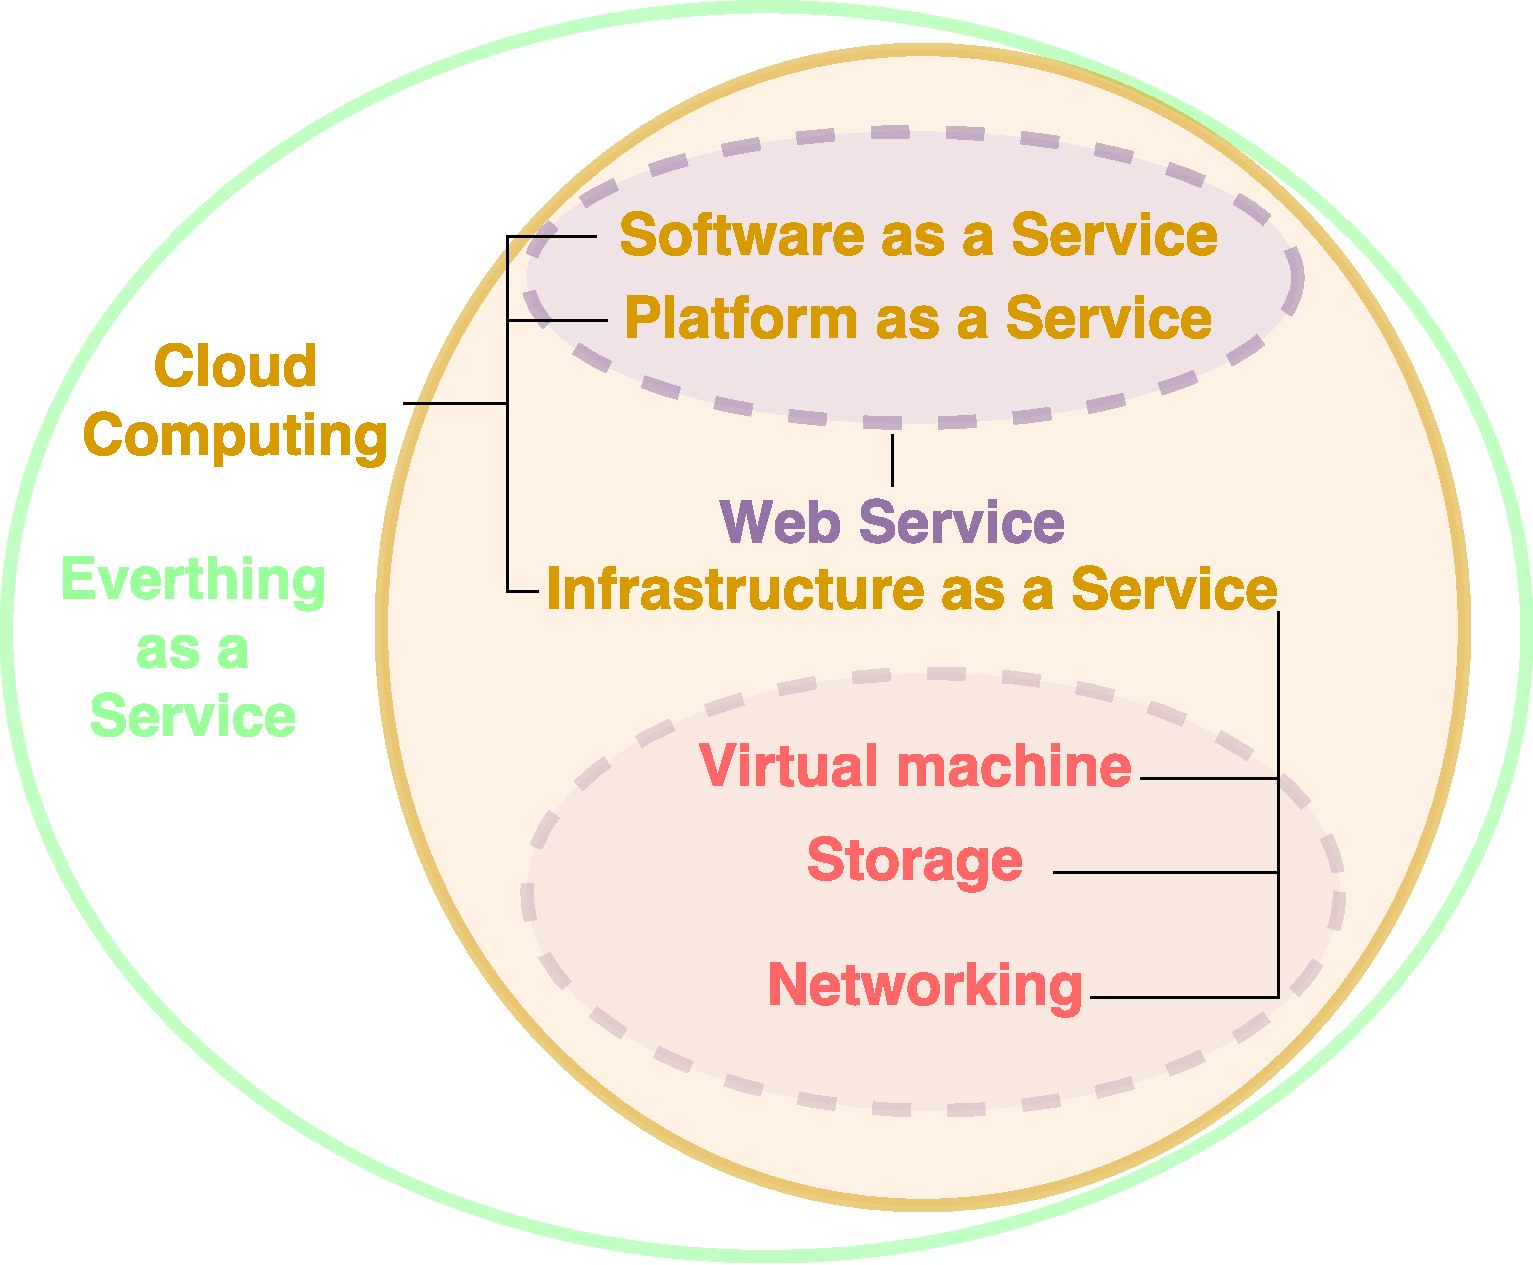
\includegraphics[width=\textwidth]{cloud_computing_venn.pdf}
  \caption{Cloud Computing.}
  \label{fig:cloud_computing}
\end{figure}

Cloud computing differs from \textbf{traditional web hosting},
mainly because of the application of visualization layer.
Visualization technology offers greater freedom resulting a
much higher scalability, and enables finer grained billing model (Pay as You Go).
see Chapter \ref{cha:system} for more information.

\textbf{Grid computing} is the collection of computer resources from multiple locations to reach a common goal. The grid can be thought of as a distributed system with non-interactive workloads that involve a large number of files \cite{grid_computing}.
In comparison, Cloud computing has more generic use cases, applicable to handle large, small or dynamic workload.

\section{Cloud Concepts}

\subsection{Virtualization}
Virtualization technique was developed in late 1990s and is different from simulation and emulation.
Virtualization employs techniques used to create instances of an environment, as opposed to simulation, which models the environment; or emulation, which replicates the target environment such as certain kind of virtual machine environment. Full virtualization requires that every salient feature of the hardware be reflected into one of several virtual machines – including the full instruction set, input/output operations, interrupts, memory access, and whatever other elements are used by the software that runs on the bare machine, and that is intended to run in a virtual machine \cite{virtualization}.

\subsection{Hypervisor}

A hypervisor is computer software, firmware that creates and runs virtual machines. A computer on which a hypervisor runs one or more virtual machines is called a host machine, and each virtual machine is called a guest machine. The hypervisor presents the guest operating systems with a virtual operating platform and manages the execution of the guest operating systems. Multiple instances of a variety of operating systems may share the virtualized hardware resources: for example, Linux, Windows, and Mac OS instances can all run on a single physical x86 machine \cite{hypervisor}. See table \ref{table:hypervisor_types} for types and examples of hypervisor.

\begin{table}
    \begin{tabular}{ p{70mm} | p{70mm} }
        \hline
        \multicolumn{2}{c}{Types of hypervisor} \\
        \hline
        Native or Bare-metal & Hosted \\
        \hline
            Run directly on the host's hardware.& 
            Run on a conventional operating system (OS)\\
        \hline
            These hypervisors run directly on the host's hardware to control the hardware and to manage guest operating systems. For this reason, they are sometimes called bare metal hypervisors.& 
            These hypervisors run on a conventional OS just as other computer programs do. A guest operating system runs as a process on the host. These hypervisors abstract guest operating systems from the host operating system.   \\
        \hline
        \multicolumn{2}{c}{Examples} \\
        \hline
            Xen \cite{Xen}, Microsoft Hyper-V \cite{Hyper-V}, VMware ESX \cite{VMware_ESXi} & 
            VMware Workstation \cite{VMware_Workstation}, VMware Player, VirtualBox \cite{VirtualBox} \\
        \hline
    \end{tabular}
    \caption{Types of hypervisor}
    \label{table:hypervisor_types}
\end{table}

\subsection{Containerization}

Operating-system-level virtualization, also known as containerization, refers to an operating system feature in which the kernel allows the existence of multiple isolated user-space instances. Such instances, called containers, may look like real computers from the point of view of programs running in them. 
A computer program running on an ordinary person's computer's operating system can see all resources (connected devices, files and folders, network shares, CPU power, quantifiable hardware capabilities) of that computer. However, programs running inside a container can only see the container's contents and devices assigned to the container \cite{containerization}.
An example implementation is Docker \cite{docker}.

\subsection{Everything as a Service}
Everything as a service (EaaS, XaaS, *aaS) is initially a concept of being able to call up re-usable, fine-grained software components across a network. The most common and successful example is software as a service, but the term as a service has been associated and used with many core components of cloud computing including communication, infrastructure, data and platforms \cite{XaaS}.

As the term getting more popular, a number of vendors including Google, Microsoft, Hewlett Packard, Amazon have been associated with the "everything as a service" trend, i.e. machine learning as a service, mobile backend as a service, mechanical turk (human as a service), security and testing as a service.

XaaS is not only limited to online services. Bricks-and-mortar businesses are also being transformed through digital connectivity. Transportation-as-a-service is being fulfilled by companies like Uber and Lyft; grocery-as-a-service is being offered by chains such as Safeway and Whole Foods; and accommodation-as-a-service is a lodging rental service provided by Airbnb. This is just the tip of the iceberg with many more on their way \cite{XaaS_beyond}.

\section{Ontological Knowledge Representation}
Many industries (i.e. smart factories, business analytics) are
becoming increasingly dependent on complex automatic software systems for tasks like resource allocation, business decision making, etc.
For example, to make decentralized decisions, those systems need to cooperate with each other as well as with humans.
However, those systems typically access data from different models.
These information models have been independently developed in different (often incompatible) formats using different types of proprietary software; furthermore, they may not come with a well-defined semantics, and their specification can be ambiguous.
As a result, model development, maintenance, and integration, as well as data exchange and sharing pose major challenges in practice
\cite{CapturingIndustrialInformationWithOntologies}.

As a result, adoption of semantic technologies has been welcomed in many large companies such as in Google, Facebook, IBM \cite{SemanticTechnologiesInIBM}
and Siemens \cite{CapturingIndustrialInformationWithOntologies}.
For example, OWL 2 ontologies are often used to capture the conceptual information models.
OWL 2 is a rich and flexible modeling language. It not only comes with an
unambiguous, standardized, semantics, but also with a wide range of tools that can be used to
develop, validate, integrate, and reason with such models.
Data can be stored in RDF triplestores and effectively queried in conjunction with the available ontologies.
RDF is a standard model for data interchange on the Web.
RDF has features that facilitate data merging even if the underlying schemas differ,
and it specifically supports the evolution of schemas over time
without requiring all data consumers to be changed \cite{RDF}.
Moreover, legacy and other data that must remain in its original format can be virtualised as RDF using ontologies.

\subsection{Terminology, Taxonomy and Ontology}
Terminology is a system or collection of words. The system is managed to make content more consistent and standardized. Terminology helps improve readability, translation, and brand perception \cite{TaxonomyVSTerminology}.

A taxonomy is a way to classify words into hierarchical groups. The biggest use of a taxonomy is for search.
A taxonomy defines groups of words. It can be multi-layered or flat \cite{TaxonomyVSTerminology}.

An ontology describes a concept both by its position in a hierarchy and its relationships to other concepts. The richness of the relationships described in an ontology is what makes more powerful for modeling complex systems \cite{OntologyHasRicherRelationshipThanTaxonomy}.

In computer-science Taxonomy has been adopted to name trees of generalization-specialization relation. In ontologies can be build over any kind of relationships, including generalization-specialization and many other.
Taxonomies and ontologies usually concern terms but they are not limited to such. In terms of graph theory, taxonomies are trees, and ontologies are graphs or hyper-graphs, where edges are build from many different relations. Those relation could have any properties according to set theory \cite{taxonomiesRtreesOntologiesRgraphs}.

\subsection{Ontology versus Database}

For those who are familiar with database, ontology axioms are like DB schema.
In database, schema describes structure of and constraints on data.
Ontology facts are like DB data, they are consistent with schema constraints \cite{OntologyLanguageTool2}.
For differences, see table \ref{table:ontology_vs_database}. 
The given examples are expressed with Description Logic, see Section \ref{sec:DL} for more details.

\begin{longtable}[ht]{| p{65mm} | p{65mm} |} 
\hline
\rowcolor{orange} Database & Ontology\\
\hline
\rowcolor{green} Closed word assumption (CWA) & Open world assumption (OWA)\\ 
Missing information treated as false & Missing information treated as unknown\\
\hline
\rowcolor{lightgray} \multicolumn{2}{|c|}{For example, we have the following facts/data:}\\
\rowcolor{lightgray} \multicolumn{2}{|c|}{HarryPotter hasFriend RonWeasley}\\
\rowcolor{lightgray} \multicolumn{2}{|c|}{HarryPotter hasFriend HermioneGranger}\\
\hline
\multicolumn{2}{|c|}{Query: Is Draco Malfoy a friend of HarryPotter?}\\
\hline
DB: No & Ontology: Don’t Know (didn’t say Draco was not Harry’s friend)\\
\hline
\rowcolor{green} Unique name assumption (UNA) & No UNA \\ 
Each individual has a single unique name & Individuals may have more than one name\\
\hline
\multicolumn{2}{|c|}{How many friends does Harry Potter have?}\\
\hline
DB: 2 & Ontology: at least 1 (Ron and Hermione may be 2 names for same person)\\
\hline
\rowcolor{green} Schema behaves as constraints on structure of data & Ontology axioms behave like implications (inference rules) \\ 
\hline
\rowcolor{lightgray} \multicolumn{2}{|c|}{For example, if we try to add new facts/data:}\\
\rowcolor{lightgray} \multicolumn{2}{|c|}{Dumbledore: Wizard}\\
\rowcolor{lightgray} \multicolumn{2}{|c|}{Fawkes: Phoenix}\\
\rowcolor{lightgray} \multicolumn{2}{|c|}{Fawkes isPetOf Dumbledore}\\
\rowcolor{lightgray} \multicolumn{2}{|c|}{$\exists hasPet.\top\subseteq Human$}\\
\rowcolor{lightgray} \multicolumn{2}{|c|}{$Phoenix\subseteq\forall isPetOf.Wizard$}\\
\hline
\rowcolor{gray} \multicolumn{2}{|l|}{Symbols}\\
\multicolumn{2}{|l|}{$\top$ \cite{top} tautology, top, Thing, most general concept}\\
\multicolumn{2}{|l|}{$\exists$ there exists at least one}\\
\multicolumn{2}{|l|}{$\subseteq$ is subset of}\\
\multicolumn{2}{|l|}{$\forall$ for all}\\
\hline
Update rejected: constraint violation. Domain of hasPet is Human; Dumbledore is not Human (CWA). &
Infer that Dumbledore is Human (domain restriction)\\ 
\hline
\rowcolor{green} \multicolumn{2}{|c|}{Query Answering Mechanism}\\
\hline
Schema plays no role & Ontology axioms play a powerful and crucial role\\
Data must explicitly satisfy schema constraints & Answer may include implicitly derived facts. Can answer conceptual as well as extensional queries, e.g., Can a Muggle have a Phoenix for a pet?\\ 
Query answering amounts to model checking, i.e., a “\textbf{look-up}” against the data & Query answering amounts to theorem proving, i.e., \textbf{logical entailment}\\ 
\textbf{Can be very efficiently implemented.} Worst case complexity is low (logspace) w.r.t. size of data. & \textbf{May have very high worst case complexity}, e.g., for OWL, NP-hard w.r.t. size of data
(upper bound is an open problem). Implementations may still behave well in typical cases.\\ 
\hline
\caption{Ontology versus Database}
\label{table:ontology_vs_database}
\end{longtable}

\subsection{Description Logic}
\label{sec:DL}

RDFS, and OWL support a family of knowledge representation languages called description logics (DL) \cite{DLExample}. A description logic can model concepts, roles and individuals, and their relationships. The common notations used in DL can be find in Table \ref{table:DL_notation}. Different DLs often with "strange names". see Table \ref{table:DL_naming_convention}
for more details, and Table \ref{table:DL_ontology_language} shows which DL is supported in which ontology language.

\begin{longtable}[h]{ p{10mm} p{60mm} p{15mm} p{45mm}}
\caption{Description Logic Notation}
\label{table:DL_notation}\\
\hline
\hline
Symbol & Description & Example & Read\\
\hline
$\top$ & tautology is a special concept with every individual as an instance, abbreviation for $A \sqcup \neg A$ for any concept A & $\top$ & top\\
\hline
$\bot$ & empty concept, contradiction, abbreviation for $A \sqcap \neg A$ for any concept A & $\bot$ & bottom\\
\hline
$\sqcap$ & intersection or conjunction of concepts & $ C \sqcap D $ & C and D\\
\hline
$\sqcup$ & union or disjunction of concepts	& $ C \sqcup D $ & C or D\\
\hline
$\neg$ & negation or complement of concepts	& $\neg C$ & not C\\
\hline
$\forall$ & universal restriction & $\forall R.C$ & all R-successors are in C\\
\hline
$\exists$ & existential restriction	& $\exists R.C$ & an R-successor exists in C\\
\hline
$\sqsubseteq$ & Concept inclusion, subclass relationship. & $ C \sqsubseteq D $ & all C are D\\
\hline
$ \equiv $ & Concept equivalence & $ C \equiv D $ &	C is equivalent to D\\
\hline
$\dot{=}$ & Concept definition & $ C \dot{=} D $ & C is defined to be equal to D\\
\hline
: &	Concept assertion & a:C & a is a C\\
\hline
: &	Role assertion & (a,b):R & a is R-related to b\\
\hline
\hline
\end{longtable}

\begin{longtable}[h]{ p{10mm} p{120mm} }
\caption{Description Logic Naming Convention: Meaning for Letters}
\label{table:DL_naming_convention}\\
\hline
Symbol & Constructs	and Example\\
\hline
$\mathcal{AL}$ & Attributive Language\\
& Atomic negation, concept intersection, universal restrictions, limited existential quantification\\
& $ copyrightHolder \equiv Organization \sqcup Person $\\
\hline
$\mathcal{C}$ & Complex concept negation\\
& Complex class expressions by combining mathematical operators such as subclass relationships, equivalence, conjunction, disjunction, negation, property restrictions, tautology, and contradiction\\
& $ cartoon \equiv animatedMovie \sqcap \neg (liveAction \sqcup computerAnimation) $\\
& Some DL languages have overlapping constructs, as, for example, union and full existential quantification can be expressed using negation, therefore $\mathcal{U}$ and $\mathcal{E}$ are never used together in DL names, and C is used instead.\\
\hline
$\mathcal{S}$ & An abbreviation for $\mathcal{ALC}$ with transitive roles\\
& $partOf \circ partOf \sqsubseteq partOf$\\
\hline
$\mathcal{E}$ &	Full existential qualification (existential restrictions that have fillers other than $\top$ )\\
& $ \exists hasDiscRelease.Blu-Ray $ \\
\hline
$\mathcal{F}$ &	Functional properties, a special case of uniqueness quantification.\\
& $ \top \sqsubseteq \leq 1$ officialWebsite$.\top $ \\
\hline
$\mathcal{U}$ &	Concept union\\
& $ broadcastChannel \equiv webcastChannel \sqcup televisionChannel $\\
\hline
$\mathcal{H}$ & Role hierarchy (subproperties: \texttt{rdfs:subPropertyOf})\\
& $ remakeOf \sqsubseteq basedOn $ \\
\hline
$\mathcal{R}$ & Limited complex role inclusion axioms; reflexivity and irreflexivity; role disjointness.\\
& $ supervisorOf \circ castMemberOf \sqsubseteq directorOf $ \\
\hline
$\mathcal{O}$ & Enumerated classes of object value restrictions (Nominals): \texttt{owl:oneOf}, \texttt{owl:hasValue}.\\
& $ AnimationStudios \equiv { DreamWorks, Walt Disney Animation Studios, Pixar }$\\
\hline
$\mathcal{I}$ &	Inverse properties.\\
& $ directedBy \approx directorOf^{-} $\\
\hline
$\mathcal{N}$ & Cardinality restrictions (\texttt{owl:cardinality}, \texttt{owl:maxCardinality}), a special case of counting quantification\\
& $ TVSeries \equiv \geq 2hasEpisode.\top $\\
\hline
$\mathcal{Q}$ & Qualified cardinality restrictions (available in OWL 2, cardinality restrictions that have fillers other than $\top$ ).\\
& $	Actor \sqsubseteq = 1hasBirthplace.Human $\\
\hline
$\mathcal{(D)}$ & Use of datatype properties, data values or data types.\\
& $\top\sqsubseteq\forall\geq 0zeroone.float$\\
& $\top\sqsubseteq\forall\leq 1zeroone.float$\\
& $\top\sqsubseteq\forall transparency.zeroone$\\
& $\exists transparency.\top \sqsubseteq Material$\\
\hline
\end{longtable}

In DL, a distinction is drawn between the so-called TBox (\textbf{terminological box}) and the ABox (\textbf{assertional box}). In general, the TBox contains sentences describing concept hierarchies (i.e., relations between concepts) while the ABox contains ground sentences stating where in the hierarchy individuals belong (i.e., relations between individuals and concepts). For example, the statement:

\blockquote{Every employee is a person}

belongs in the TBox, while the statement:

\blockquote{Bob is an employee}

belongs in the ABox.

A Knowledge Base (KB) is just a TBox plus an Abox, see section \ref{sec:KB} for more details about KB.

\begin{longtable}[h]{ p{20mm} p{110mm} }
\caption{Description Logic and Ontology Languages}
\label{table:DL_ontology_language}\\
\hline
Ontology Language & Description Logic\\
\hline
OWL Lite & equally expressive as $\mathcal{SHIF(D)}$\\
& extending $\mathcal{ALC}$ with transitivity roles (i.e., $\mathcal{S}$) with role hierarchies ($\mathcal{H}$), inverse roles ($\mathcal{I}$), functional properties ($\mathcal{F}$), and datatypes $\mathcal{(D)}$\\
\hline
OWL DL & equally expressive as $\mathcal{SHOIN(D)}$\\
& adding nominals ($\mathcal{O}$) and cardinality restrictions ($\mathcal{N}$) to $\mathcal{SHIF(D)}$\\
\hline
OWL 2 DL & equally expressive as $\mathcal{SROIQ(D)}$\\
& After industrial applications highlighted several key features missing from $\mathcal{SHOIN(D)}$ to model complex knowledge domains, $\mathcal{SHOIN(D)}$ has been extended with complex role inclusion axioms, reflexive and irreflexive roles, asymmetric roles, disjoint roles, the universal role, self-constructs, negated role assertions, and qualified number restrictions, leading to $\mathcal{SROIQ(D)}$, one of the most expressive description logic whose decidability is proven. Furthermore, $\mathcal{SROIQ(D)}$ supports not only TBox and ABox axioms, but also so-called Role Boxes (RBox) to collect all statements related to roles and the interdependencies between roles.\\
\hline
\end{longtable}

Description logics are also used in artificial intelligence to describe and reason about the relevant concepts of an application domain (known as terminological knowledge). The most notable application of DLs and OWL is in biomedical informatics where DL assists in the codification of biomedical knowledge \cite{Description_logic}.

Many description logics are \textbf{decidable} fragments of first-order logic (FOL), also known as first-order predicate calculus (FOPC) \cite{DL_FOL}, see Section \ref{sec:FOL} for more details. 
Table \ref{table:FOL_DL} shows some translation examples between DL and FOL.

In logic, the term decidable refers to the decision problem, the question of the existence of an effective method for determining membership in a set of formulas, or, more precisely, an algorithm that can and will return a boolean true or false value that is correct (instead of looping indefinitely, crashing, returning "don't know" or returning a wrong answer). Logical systems such as propositional logic are decidable if membership in their set of logically valid formulas (or theorems) can be effectively determined. A theory (set of sentences closed under logical consequence) in a fixed logical system is decidable if there is an effective method for determining whether arbitrary formulas are included in the theory. Many important problems are undecidable, that is, it has been proven that no effective method for determining membership (returning a correct answer after finite, though possibly very long, time in all cases) can exist for them \cite{Decidability}.

\begin{longtable}[h]{ p{65mm} p{65mm} }
\caption{FOL and DL}
\label{table:FOL_DL}\\
\hline
First-Order Logic & Description Logic\\
\hline
C(a) & C(a), alternatively a : C\\
$A \approx B$ & $A \equiv B$\\
$\neg C(x)$ & $\neg C$\\
$C(x) \land D(x)$ &	$C \sqcap D$\\
$C(x) \lor D(x)$ & $C \sqcup D$\\
$\forall x(C(x) \rightarrow D(x))$ & $C \sqsubseteq D$\\
R(a,b) & R(a,b), alternatively (a,b) : R\\
$\forall x \forall y(R(x,y) \rightarrow S(x,y))$ & $R \sqsubseteq S$\\
$\exists y(R(x,y) \land C(y))$ & $\exists R.C$\\
$\forall x \forall y \forall z(R(x,y) \rightarrow R(y,z) \rightarrow R(x,z))$ & $R \circ R \sqsubseteq R$\\
\hline
\end{longtable}

Description logic-based knowledge representations not only store human knowledge in a machine-readable form, but also provide the option to automatically infer new RDF statements via reasoning, find contradictory statements in a knowledge base if any (consistency checking), and determine concept satisfiability, i.e., check whether a concept can ever have instances, see section \ref{sec:satisfiability_decidability} for more detail. These tasks are usually performed with reference to a knowledge base or a TBox.

The visualization of the hierarchy of the subclass-superclass relationships between concepts, called the subsumption hierarchy, provides the option to easily overview the knowledge domain model. Consequently, calculating the subsumption hierarchy is one of the most common reasoning tasks\cite{DLReasoning}.

\subsection{First Order Logic}
\label{sec:FOL}

In FOL, the semantics is defined in terms of models. A model is 
supposed to be an analogue of (part of) the world being modeled. FOL uses a very
simple kind of model, in which “objects” in the world (not necessarily physical objects)
are modeled as elements of a set, and relationships between objects are modeled as
sets of tuples\cite{OntologyLanguageTool1}.
Note that this is exactly the same kind of
model as used in a database: objects in the
world are modeled as values (elements) and
relationships as tables (sets of tuples). 

See Figure \ref{fig:FOL} as an example.
Model: a pair $<D, .^{I}>$ with D a non-empty set and 
$.^{I}$ an interpretation.
An interpretation \cite{Interpretation} is an assignment of meaning to the symbols of a formal language. Many formal languages used in mathematics, logic, and theoretical computer science are defined in solely syntactic terms, and as such do not have any meaning until they are given some interpretation. 
$v^{I}$ is an element of D.

\begin{figure}[h]
  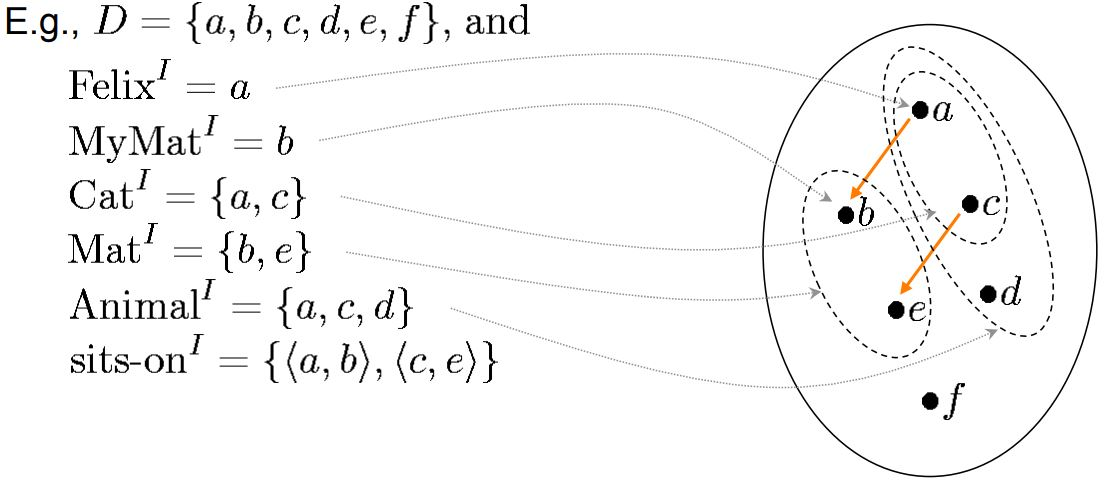
\includegraphics[width=\textwidth]{FOL.JPG}
  \caption{First-order Logic}
  \label{fig:FOL}
\end{figure}

Table \ref{table:FOL_truth_evaluation} shows some truth value evaluation examples in the above given model $M = <D, .^{I}>$, see figure \ref{fig:FOL} for model definition.

\begin{longtable}[h]{ p{100mm} p{30mm} }
\caption{FOL Truth value evaluation}
\label{table:FOL_truth_evaluation}\\
\hline
Statement & Evaluation\\
\hline
$\exists x.Cat(x)$ & true\\
$\forall x.Cat(x)$ & false\\
$\exists x.Cat(x) \land Mat(x)$ & false\\
$\forall x.Cat(x) \rightarrow Animal(x)$ & true\\
$\forall x.Cat(x) \rightarrow (\exists y.Mat(y) \land sits-on(x,y))$ & true\\
\hline
\end{longtable}

\subsubsection{Satisfiability and Decidability}
\label{sec:satisfiability_decidability}

Given a model M and a formula F, M is a model of F (written $M \models F$) iff F evaluates to true in M.
See examples below.

$M \models \exists x.Cat(x)$

$M \not\models \forall x.Cat(x)$

$M \not\models \exists x.Cat(x) \land Mat(x)$

$M \models \forall x.Cat(x) \rightarrow Animal(x)$

$M \models \forall x.Cat(x) \rightarrow (\exists y.Mat(y) \land sits-on(x,y))$

A formula F is \textbf{satisfiable} iff there exists a model M s.t. $M \models F$.

A formula F \textbf{entails} another formula G (written $F \models G$) iff every model of F 
is also a model of G (i.e., $M \models F$ implies $M \models G$). 

Satisfiable examples:

$Cat(Felix) \models \exists x.Cat(x)$

$(\forall x.Cat(x) \rightarrow Animal(x)) \land Cat(Felix) \models Animal(Felix)$

$(\forall x.Cat(x) \rightarrow Animal(x)) \land \neg Animal(Felix) \models \neg Cat(Felix)$

Not satisfiable:

$Cat(Felix) \models \forall x.Cat(x)$

$sits-on(Felix, Mat1) \land sits-on(Tiddles, Mat2) \models \neg sits-on(Felix, Mat2)$

$sits-on(Felix, Mat1) \land sits-on(Tiddles, Mat1) \models \exists^{\geq 2} x.sits-on(x, Mat1)$

Satisfiability in the first-order logic is undecidable, i.e. no algorithm can decide correctly whether a given first-order formula is true or not. However, for any single statement $\varphi$ it is easy to come up with an algorithm that decides $\varphi$ correctly (just hard-code the answer). 
You can encode the statement \textbf{"the Turing machine T halts on empty input"} in first-order logic, this statement is already undecidable, that is, no algorithm can correctly decide whether such a formula is true or not, 
see section \ref{sec:halting_problem} about why. 
Other logics (propositional logic, DL) is decidable because they don't have the power to encode such statement \cite{30672}.

Example decidable fragments: FOL with Counting quantifiers ($\exists^{\geq n}, \exists^{\leq n}$)

$\exists^{\geq 3}x.Cat(x)$ equivalent to

$\exists x,y,z.Cat(x) \land Cat(y) \land Cat(z) \land x \neq y \land x \neq z \land y \neq z $

$\exists^{\leq 2}x.Cat(x)$ equivalent to

$\forall x,y,z.Cat(x) \land Cat(y) \land Cat(z) \rightarrow x=y \lor x=z \lor y=z $

\subsubsection{Halting Problem}
\label{sec:halting_problem}
In computability theory, the halting problem is the problem of determining, from a description of an arbitrary computer program and an input, whether the program will finish running or continue to run forever.

Alan Turing proved in 1936 that a general algorithm to solve the halting problem for all possible program-input pairs cannot exist. A key part of the proof was a mathematical definition of a computer and program, which became known as a Turing machine; the halting problem is undecidable over Turing machines. It is one of the first examples of a decision problem \cite{halting_problem}.

Proof by contradiction:
Suppose that there exists a total computable function \textbf{halts(g)} that returns true if the subroutine g halts (when run with no inputs) and returns false otherwise. Now consider the following subroutine:
\begin{lstlisting}
def g():
    if halts(g):
        loop_forever()
\end{lstlisting}
\textbf{halts(g)} must either return true or false, because halts was assumed to be total. 
If \textbf{halts(g)} returns true, then g will call \textbf{loop\textunderscore forever} 
and never halt, which is a contradiction. 
If \textbf{halts(g)} returns false, then g will halt, 
because it will not call \textbf{loop\textunderscore forever}; this is also a contradiction. 
Overall, \textbf{halts(g)} can not return a truth value that is consistent with whether g halts. 
Therefore, the initial assumption that halts is a total computable function must be false.

\subsection{Knowledge Base}
\label{sec:KB}

A knowledge base (KB) \cite{knowledge_base} is a technology used to store complex structured and unstructured information used by a computer system. A knowledge-based system consists of a knowledge-base that represents facts about the world and an inference engine \cite{jena} that can reason about those facts and use rules and other forms of logic to deduce new facts or highlight inconsistencies.

The term "knowledge-base" was coined to distinguish this form of knowledge store from the more common and widely used term database. At the time (the 1970s) virtually all large Management Information Systems stored their data in some type of hierarchical or relational database. At this point in the history of Information Technology the distinction between a database and a knowledge base was clear and unambiguous. A database had ACID transaction properties: Atomicity, Consistency, Isolation, and Durability. Early expert systems had little need for the complexity that comes with requiring transactional properties on data. 

The volume requirements were also different for a knowledge-base compared to a conventional database. The knowledge-base needed to know facts about the world. For example, to represent the statement that "All humans are mortal". A database typically could not represent this general knowledge but instead would need to store information about thousands of tables that represented information about specific humans. Representing that all humans are mortal and being able to reason about any given human that they are mortal is the work of a knowledge-base. Representing that George, Mary, Sam, Jenna, Mike,... and hundreds of thousands of other customers are all humans with specific ages, sex, address, etc. is the work for a database.

The next evolution for the term knowledge-base was the Internet. With the rise of the Internet, documents, hypertext, and multimedia support were now critical for any corporate database. It was no longer enough to support large tables of data or relatively small objects that lived primarily in computer memory. 

Knowledge Base Consistency Checking:
Given knowledge base K as input, a decision procedure for knowledge base consistency returns “K is consistent” if there is an interpretation I such that $I \models K$, otherwise it returns “K is inconsistent.” \cite{KnowledgeBaseConsistency}, see section \ref{sec:satisfiability_decidability} for more definitions. 

\subsection{Linked Data}

In computing, linked data (often capitalized as Linked Data) is a method of publishing structured data so that it can be interlinked and become more useful through semantic queries. It builds upon standard Web technologies such as HTTP, RDF and URIs, but rather than using them to serve web pages for human readers, it extends them to share information in a way that can be read automatically by computers.

Tim Berners-Lee, director of the World Wide Web Consortium (W3C), coined the term in a 2006 design note about the Semantic Web project \cite{LinkedData}. Linked data may also be open data, in which case it is usually described as linked open data (LOD).

Some example Resource Description Framework serialization formats are RDF/XML, JSON-LD \cite{JSON-LD} . 

Some example Datasets (knowledge base):

\begin{enumerate}
    % 1
    \item 
    DBpedia – a dataset containing extracted data from Wikipedia; it contains about 3.4 million concepts described by 1 billion triples, including abstracts in 11 different languages.
    % 2
    \item
    FOAF \cite{FOAF} – a dataset describing persons, their properties and relationships.
    % 3
    \item
    GeoNames provides RDF descriptions of more than 7,500,000 geographical features worldwide.
     % 4
    \item
    Wikidata – a collaboratively-created linked dataset that acts as central storage for the structured data of its Wikimedia Foundation sister projects.In 2014, Freebase \cite{Freebase} merged into Wikidata, Google's Knowledge Graph was powered in part by Freebase.
\end{enumerate}

\subsection{Schema.org and Google Knowledge Graph}

Schema.org \cite{Schema.org} is an initiative launched on 2 June 2011 by Bing, Google and Yahoo to "create and support a common set of schemas for structured data markup on web pages." In November 2011 Yandex (whose search engine is the largest one in Russia) joined the initiative.

The Knowledge Graph is a knowledge base used by Google and its services to enhance its search engine's results with information gathered from a variety of sources. This information is presented to users in a box to the right of search results. Knowledge Graph boxes were added to Google's search engine in May 2012. The information covered by the Knowledge Graph grew significantly after launch, tripling its original size within seven months, and being able to answer "roughly one-third" of the 100 billion monthly searches Google processed in May 2016 \cite{Knowledge_Graph}.
In October 2016, Google announced that the Knowledge Graph held over 70 billion facts. The information is often used as a spoken answer in Google Assistant and Google Home searches. 

The Knowledge Graph Search API uses standard schema.org types and is compliant with the JSON-LD specification.

The Knowledge Graph has been criticized for providing answers without source attribution.

\subsection{RDF}
\label{sec:RDF}
The purpose of RDF is to provide a structure (aka framework)
for describing identified things (aka resources) \cite{RDFandOWL_SenmanticWebAffinityGroup}.
The RDF data model is based on statements to describe and feature resources, especially web resources, in the form of subject-predicate-object (resource–property–value) expressions (RDF triples) \cite{rdf-triples}.

Structured datasets can be written in RDF using a variety of other syntax notations and data serialization formats, for example, RDFa, JSON-LD, Notation3 (N3), Turtle \cite{rdfTurtle}, etc. The N3 syntax is, for example, less verbose than the RDF/XML serialization. A subset of N3 is the Terse RDF Triple Language, often referred to as Turtle. Turtle provides a syntax to describe RDF graphs in a compact textual form, which is easy to develop. It is a subset of Notation 3 (N3) and a superset of N-Triples. Turtle is popular among Semantic Web developers and considered as an easy-to-read alternative to RDF/XML. The typical file extension of Turtle files is \texttt{.ttl}. The character encoding of Turtle files should be \texttt{UTF-8}. The MIME type of Turtle is \texttt{text/turtle}. Turtle is supported by many software frameworks that can be used for querying and analyzing RDF data, such as Jena and Sesame. Turtle files consist of a sequence of directives, statements representing triples, and blank lines.

\subsection{RDFS}
As mentioned in Section \ref{sec:RDF}, RDF allows you to link resources (concepts) together so you could say that (Karthik  is a person). Think about it as directed graph, however you can't classify objects so you can't say for example that person is a subclass of human-beings.

RDFS (RDF Schema) gives you more expressive vocabulary, this means you can start making statements about classes of thing, and types of relationship. It also allows you to describe in human readable text the meaning of a relationship or a class.
It allows you to classify resources by using the class and subclass (\texttt{rdfs:class}, \texttt{rdfs:subclass}) notions. It also allows you to set restriction on the properties(relationships) using \texttt{rdfs:Domain} and texttt{rdfs:range}.
It tells you legal uses of various classes and relationships. It is also used to indicate that a class or property is a sub-type of a more general type. For example "HumanParent" is a subclass of "Person". "Loves" is a sub-class of "Knows"\cite{RDFvsOWL_SO}.

\subsection{OWL}
The purpose of OWL is to develop ontologies that are compatible with the World Wide Web \cite{RDFandOWL_SenmanticWebAffinityGroup}.
OWL it is closely related to it to RDF, however, OWL is not an extension to RDF, in the same sense that DTDs and XML Schema are not extensions to XML \cite{RDFvsOWLquora}. 
OWL is a way of adding meaning / semantic richness to RDF.  Among other things this allows automated reasoning / influencing.
OWL is a way to define types for RDF data, though OWL "typing"  differs from conventional type systems in that it has an open world  assumption. OWL is represented using RDF triples and typically expressed using RDF/XML syntax.
OWL allows you to add more restrictions. It categorises properties(relationships) into object and data properties and allows you to add restrictions on your properties.

\subsection{Ontology Design Pattern}
Like the software design patterns, many Ontology design patterns(ODP) \cite{ODP}
also have been proposed to suggest standardized solutions for common problems.

\subsection{Related Research}
The research group of the Department of Soft Computing and Intelligent Information Systems
at the University of Granada \cite{DataMiningServicedefinitionInCloud}, 
has developed two small Cloud ontologies.
The set of concepts and features they covered are limited and as a result, their examples are limited to some simple cases.
For instance, the examples presented in Section \ref{sec:PriceSpecification}
can not be modeled with their ontologies.
Since their data-sets link are now inaccessible,
there is no further evidence of the applicability of their model today.

K. Boukadi et al. developed a Cloud Service Description Ontology (CSO) \cite{Boukadi2016CloudSD}, where they model a Cloud Service brokerage. The the price model is overly simplified, compared to real word scenarios. Their model and data is also not available online to evaluate it further or to reuse it in other contexts.

The mOSAIC project \cite{Moscato2011AnAO} proposed an OWL ontology for Cloud services negotiation (i.e. between costumer and provider) and composition (i.e. by an administrator). They have a very different scope.

K. Joshi et al. developed an OWL Ontology for the Lifecycle of IT Services in the
Cloud \cite{Joshi2014AutomatingCS}. It models the steps involved in the
phases of discovery, negotiation, composition, and consumption of Cloud Service.
The Cloud service features modelled are very limited, link to an example of a
storage service \cite{kjoshi_storage_ontology} is no longer accessible.

Overall, these other research projects had different focuses. 
Our focus is on modeling realistic price specifications of cloud service and their  features, 
but models for orchestration \cite{Moscato2011AnAO,Joshi2014AutomatingCS} or
brokerage processes \cite{Boukadi2016CloudSD} are outside of the scope of the proposed ontology. However, our ontology could be extended in this regard using the models proposed in these works.
The rest of the projects \cite{Boukadi2016CloudSD,Moscato2011AnAO}
do not make their model and data available, and hence are not easy to use or to replicate their results and require a significant mapping effort in their adoption (mapping to real service data).
To address the issue of mapping to real word data, we also developed tools for automatically converting data from provider API's to RDF data for our use cases. These mapping tools are also easily extensible to cover scenarios outside the one's presented in this thesis.

\section{Web Service Discovery Techniques}
\label{sec:WebServiceDiscoveryTechniques}
We surveyed a list of state of the art in Service Selection and Comparison techniques, we highlight their significant limitations, their relationship and dependency on some of the prior concepts from other fields in computing. 

\subsection{Historical Web Service Discovery}
There are a lot research in \textbf{web} service discovery. Example products of such research includes \textbf{Semantic Web},  Web Services Description Language (\textbf{WSDL}) and Universal Description, Discovery, and Integration (\textbf{UDDI}). Among those, UDDI has not been as widely adopted as its designers had hoped. It has been closed. On the other hand, Semantic Web is still very active. 

According to the W3C, "The Semantic Web provides a common framework that allows data to be shared and reused across application, enterprise, and community boundaries". The term was coined by Tim Berners-Lee for a web of data that can be processed by machines — that is, one in which much of the meaning is machine-readable. While its critics have questioned its feasibility, proponents argue that applications in industry, biology and human sciences research have already proven the validity of the original concept \cite{SemanticWeb}.

The term "Semantic Web" is often used more specifically to refer to the formats and technologies that enable it. The collection, structuring and recovery of linked data are enabled by technologies that provide a formal description of concepts, terms, and relationships within a given knowledge domain. These technologies are specified as W3C standards and some examples are:

\begin{enumerate}
    % 1
    \item 
    Resource Description Framework (RDF), a general method for describing information.
    % 2
    \item
    SPARQL, an RDF query language.
    % 3
    \item
    Web Ontology Language (OWL), a family of knowledge representation languages. For adding meaning to web content by annotating it with terms defined in ontologies.Supported by tools (e.g. Protégé) and APIs (e.g. OWL API). Based on Description Logics \cite{OntologyLanguageTool2}.
\end{enumerate}

Some of the "Cloud discovery" research just focused on the SaaS and PaaS domain, which I consider mostly can be categorized into web service discovery research. Other research projects may have included IaaS, but have over simplified the billing model or offering types, see section \ref{sec:research_problem} for more details about the complexity of those Cloud IaaS offers, thus impractical for real life scenarios. Some examples are:

\begin{enumerate}
    % 1
    \item  
    Efficient Service Discovery for Cloud Computing Environments
    \cite{EfficientServiceDiscoveryforCloudComputingEnvironments}, 
    semantics-based discovery using ontology and UDDI. Capture Cloud services details features with Web Services Description Language(WSDL) and publishing them on the web service registry (UDDI).
    But UDDI is dead.
    % 2
    \item
    Cloudle \cite{Cloudle, CloudleAgent-BasedCloudComputing}, Cloud services search engine, uses web crawler agent, ontology, k-means clustering algorithm to discover services over the Internet. 
    The proposed system was evaluated using virtual (provider) websites, how well it process real websites is questionable. Besides, Cloud providers still need to register their services in a central database. Also Cloudle's similarity is calculated on very limited number of attributes (10), a real word offer can consist many times more attributes, which may result in inaccurate clustering.
    % 3
    \item
    Integrating intelligent agent and ontology for services discovery on cloud environment
    \cite{IntelligentAgentOntologyServicesDiscovery}, the proposed framework utilizes mobile agents with ontology for searching appropriate services in cloud environment, inference rules are defined and executed by Jena engine \cite{jena} in a mobile reasoner.Mobile agents are implemented using JAVA Agent DEvelopment Framework (JADE).
    Despite the different method for retrieving information, the evaluation does not demonstrate much superiority compare to other researches. It achieves no more than 40 percent recall, means it can only retrieve 40 percent of what should be discovered (with human review).
    % 4
    \item
    OWL-S Based Semantic Cloud Service Broker \cite{OWL-CloudServiceBroker}, semantics OWL-based service broker.
    Shared ontology among cloud providers is needed to be implemented for translating the offered and requested services. QoS parameters are not included.
    % 5
    \item 
    A Cloud computing approach based on mobile agents for Web services discovery
    \cite{MobileAgentsWebServicesDiscovery}, a Keywords-based search implemented using mobile agents.    
    % 6
    \item
    Ontology-based annotation and retrieval of services in the cloud \cite{Ontology-basedAnnotationRetrievalOfServicesInCloud}.
    % 7
    \item
    A Crawler Engine for Cloud Services Discovery on the World Wide Web \cite{CSCE}.
    % 8
    \item
    A semantic-based Software-as-a-Service (SaaS) discovery and selection system \cite{SaaSdiscoverySelectionSystem}.
    % 9
    \item
    Toward dynamic and attribute based publication, discovery and selection for cloud computing \cite{DynamicAttributeBasedPublicationDiscoverySelectionForCloud}, introduced a semantic schema for service publication discovery and selection.
    % 10
    \item
    Semantic Discovery of Cloud Service Catalog Published Over Resource Description Framework \cite{Vasudevan2014SemanticDO}, Semantic Discovery based on RDF.
    % 11
    \item
    Design and Implementation of the Hadoop-Based Crawler for SaaS Service Discovery \cite{Hadoop-BasedCrawlerForSaaSDiscovery}.
    % 12
    \item
    Integrating Software Agents and Web Services in Service Oriented Architecture Based Cloud Services Discovery Framework \cite{AgentSOAServicesDiscovery}.
    % 13
    \item
    A Multi-agent-Based Framework for Cloud Service Description and Discovery Using Ontology \cite{Multi-agent-BasedCloudDescriptionDiscoveryOntology}.
    % 14
    \item
    Automatic Extraction of Metrics from SLAs for Cloud Service Management \cite{AutoExtractionSLA}.
    % 15
    \item
	A Cloud Repository and Discovery Framework Based on a Unified Business and Cloud Service Ontology \cite{CloudRepositoryDiscoveryFrameworkBasedonOntology}.
\end{enumerate}

I have included a summary table about some limitations of the above projects, please see Table \ref{table:related_work} for more details. Overall, projects included in this section do not provide more comprehensive comparison, neither include QoS into comparison. There is no reference to the code base of the implemented systems, it's impossible to reproduce results and little provide evaluation on real word data.

\subsection{IaaS Pricing Calculation}

Although branded calculators are available from individual cloud providers
\cite{AWSCalculator, AzurePricingCalculator, GooglePricingCalculator, RackspaceCalculator, SoftLayerCalculator}
for calculating the service leasing cost, it is not easy for users to
generalize their requirements to fit different service offers (with
various quota and limitations), let alone compute and compare
costs. 

It's hard to do decent comparison, due to the very different nature of what things are part of billing and how they are part of billing. For some, a year consists of 365 days, for others it's only 360. While it is great that Cloud vendors provide an API for pricing estimation and calculation, the very different nature of the offerings themselves make it very hard to compare them \cite{Cloudorado}.

\subsection{Other Commercial Offers} 

The key features distinguish our solution to exiting commercial offers
\cite{BurstormRecommendation, CloudHarmonyProviderDirectory, RightscaleCloudPricingService, Cloudorado, CloudReviews} 
is the application of AHP-based decision making technique
and Queuing Theory based QoS modeling in our algorithm.

\subsection{Research Works}

Swinburne University has a research project called 
Smart Cloud Broker Service \cite{OpenMarketforTradingCloudServices}.
From the screen-cast they released, we can tell that their
benchmarking is done in real time, which means that users
have to wait for the results to come back. We have considered
this kind of situation but decided to collect the benchmarking
result beforehand. This is because this way, no matter how
many cloud providers users want to compare against, they can
still get the result with minimum (or no) waiting time. Another
reason we choose to do it this way is because, at any particular
point in time, the network benchmark result is not conclusive as
performance fluctuates during time; thus, we use an aggregated
average, which is a more reliable overall indication.

Menzel and Ranjan introduced a framework called
“CloudGenius” \cite{CloudGenius} that supports a decision-making process on web
server migration into the cloud. Our system supplements and
partially extends their work. CloudGenius \cite{CloudGenius} focuses on
VM selection, which means that it considers the software requirements
(i.e., the operating system version and the supported
languages), but our study focuses more on the hardware requirements
(i.e., the size of memory and hard disk). Although we
have borrowed the idea of using the AHP (with modification) from CloudGenius,
we used it differently. We have implement the method while following the declarative programming
paradigm, which should be easier to scale out as opposed to rewriting an imperative code implementation.

There are methods proposed for network-aware service composition
\cite{Yu2007, Benatallah2004, Zheng2013}
considering a generic web service, i.e., at the
Software-as-a-Service and Platform-as-a-Service levels. However,
the compatibility constraints at the IaaS level are different
from those at the web service. For example, generic web
services are distinguished by their features, QoS, and prices.
It does not make sense to include two exact same services in
one composition as one job does not need to be done twice, but
using multiple quantities of an IaaS offer is perfectly valid.

\subsection{Summary}

\begin{longtable}{ p{30mm} | p{50mm} | p{50mm} } 
\caption{Related work \label{table:related_work}} \\
\hline
\multicolumn{3}{c}{ \cellcolor{yellow} Fully Automatic Service Discovery Techniques}\\
\hline
\multicolumn{3}{p{140mm}}{All fully automatic techniques facing the same challenge of natural language processing, thus only a limited set of attributes can be captured by the proposed ontologies, and most research can only offer keyword based search, or does not consider service performance.}\\
\hline
Research Title & Proposed Method & Limitation \\ 
\hline
	A semantic-based Software-as-a-Service (SaaS) discovery and selection system \cite{SaaSdiscoverySelectionSystem}. &
    Offers text/term based search. Firstly, Cloud service providers register their services, this data is  processed by consulting the WordNet \cite{WordNet} ontology to expand the service description using the token synonyms, it is  then stored in their proposed ontology. TFIDF algorithm is used to calculate weight vector for each service, then the cosine similarity between those vectors are calculated, finally the agglomerative clustering algorithm is applied to categorize services based on similarity.&
    Despite all the information retrieval techniques applied, it still requires service providers to register themselves manually. \\
\hline
	Semantic Discovery of Cloud Service Catalog Published Over Resource Description Framework \cite{Vasudevan2014SemanticDO} &
    Semantic Discovery based on RDF. String similarity is calculated by Levenshtein (edit) distance. Concept  similarity is calculated by finding the Least Common Hypernym (LCH) in WordNet \cite{WordNet}.The system was implemented with the Jena inference rules engine \cite{jena}.&
    Missing key references such as: which ReVerb did they use, making it hard to evaluate and reproduce the work.\\
\hline
	Integrating intelligent agent and ontology for services discovery on cloud environment
    \cite{IntelligentAgentOntologyServicesDiscovery} & 
    Integrating mobile agents with ontology for searching cloud services
    using inference rules executed by Jena engine \cite{jena}.& 
    Despite the different method for retrieving information, the evaluation does not demonstrate much superiority compare to other researches. It achieves no more than 40 percent recall, means it can only retrieve 40 percent of what should be discovered (with human review).\\ 
\hline
	OWL-S Based Semantic Cloud Service Broker \cite{OWL-CloudServiceBroker}&
    semantics OWL-based service broker.&
    Shared ontology among cloud providers is needed to be implemented for translating the offered and requested services. QoS parameters are not included.\\
\hline
    A Cloud computing approach based on mobile agents for Web services discovery
    \cite{MobileAgentsWebServicesDiscovery}&
    Crawling information using mobile agents, keyword-based search is used to compare between user request and cloud service description.& 
    It does not cover numeric attributes such as cost and performance.\\
\hline
    Ontology-based annotation and retrieval of services in the cloud \cite{Ontology-basedAnnotationRetrievalOfServicesInCloud}&
    Annotates cloud services descriptions in natural language using semantic techniques such as TFIDF (term frequency inverse document frequency algorithm) and ontology (OWL2).&
    It only covers a few attributes. The validation of the system was performed on a small set of services without statistical analysis on large data sets.\\
\hline
	A Crawler Engine for Cloud Services Discovery on the World Wide Web \cite{CSCE} &
    Crawl cloud web portals and store the retrieved Cloud services information in a local repository. The collected Cloud services were categorized into IaaS, PaaS and SaaS based on Ontology.&
    This research is mainly addressing the entry point problem for fully automatic discovery, the data collected from each service are limited, thus there is no mentioning of addressing the more complex need of comparing services, or filter service on certain attributes (price, VM type and RAM or performance).\\
\hline
	Design and Implementation of the Hadoop-Based Crawler for SaaS Service Discovery \cite{Hadoop-BasedCrawlerForSaaSDiscovery}.&
    Hadoop framework \cite{Hadoop} based crawler, implemented with Solr search platform \citet{ApacheSolr}.&
    Do not distinguish between IaaS, PaaS or SaaS. \\
\hline
	Integrating Software Agents and Web Services in Service Oriented Architecture Based Cloud Services Discovery Framework \cite{AgentSOAServicesDiscovery}.&
	Multi agent system for Cloud service discovery and ranking following the Service Oriented Architecture \cite{SOA}. &
    Didn't include design or method on how to implement a system follow the proposed architecture. It is critical because, tasks such as generate taxonomy tree, similarity reasoning, measure documentation and compliance, evaluate client source code, can be very complex subsystem/subproblem on its own, without a concrete ground the proposed system can not be fully realized.\\
\hline
	Automatic Extraction of Metrics from SLAs for Cloud Service Management \cite{AutoExtractionSLA}&
    A prototype system, which automatically extracted the terms defined and measures of SLA documents written in text files. The extracted terms are saved as RDF graph to represent the knowledge base. &
    It covers SAL only. It does not provide a comparison of SLA among different providers.\\
\hline
	CSRecommender \cite{CSRecommender}&
    A search engine system called CSRecommender optimised especially for cloud services. It identifies some interested sites to crawl their web pages,
    a score is assigned to each page based on key word frequencies (i.e. TFIDF is used). It also collected users rating on the search result, to improve the recommendation relevance.&
    It was applied on few cloud services. Accuracy is low. It does not cover all types of Cloud services.\\
\hline
% Semi-automatic Service Discovery 
\multicolumn{3}{c}{\cellcolor{yellow} Semi-automatic Service Discovery with More Complex Filtering}\\
\hline
Research Title & Proposed Method & Limitation \\
\hline
	A Cloud Repository and Discovery Framework Based on a Unified Business and Cloud Service Ontology \cite{CloudRepositoryDiscoveryFrameworkBasedonOntology}&
    A framework that served as a services repository. It provides an integrated, unified business service and cloud ontology to help organizations to discover suitable cloud services using querying abilities. &
    The equalization between the query and business function asked by the user. The SPARQL query language was mainly comprehensive to expert users only. No evaluation on real market data, result only shows a mock-up "Selected Cloud provider".\\
\hline
    A Multi-agent-Based Framework for Cloud Service Description and Discovery Using Ontology \cite{Multi-agent-BasedCloudDescriptionDiscoveryOntology}&
    A prototype system for describing and discovering Cloud services, based on ontology and agents.&
    Requires service provider to implement agent system to interact with service registry. No evaluation with real data.\\
\hline
	Toward dynamic and attribute based publication, discovery and selection for cloud computing \cite{DynamicAttributeBasedPublicationDiscoverySelectionForCloud} &
    A semantic schema extending WSDL, by adding attributes for describing current state of the services, e.g. Amount of free disk space or memory, Number of processes running, percent of CPU used. &
    Because of the tightly coupling with the Web Service SOAP technology stack, there is limited application on its own, SOAP is a bit out dated compare to more recent technologies. \\
\hline   
    Efficient Service Discovery for Cloud Computing Environments
    \cite{EfficientServiceDiscoveryforCloudComputingEnvironments} & 
    Store Cloud service in WSDL file for publishing in an UDDI directory.& 
    UDDI is an old (outdated) technology and abandoned by market and community.\\ 
\hline
	Cloudle \cite{Cloudle, CloudleAgent-BasedCloudComputing} & 
    Uses agents, ontology, k-means clustering algorithm to discover services over the Internet. & 
    Evaluated using virtual (provider) websites. 
    Cloud providers still need to register their services in a central database.
    Cloud ontology only covers limited attributes,
    which will affect the similarity calculated between Cloud services.\\ 
\hline
% Web service composition 
\multicolumn{3}{c}{ \cellcolor{yellow} Web Service Composition}\\
\hline
\multicolumn{3}{p{140mm}}{There are methods proposed for network-aware service composition
\cite{Yu2007, Benatallah2004, Zheng2013}
considering generic web services, i.e., at the
Software-as-a-Service and Platform-as-a-Service levels. However,
the compatibility constraints at the IaaS level are different
from those at the web service. For example, generic web
services are distinguished by their features, QoS, and prices.
It does not make sense to include two exact same services in
one composition as one job does not need to be done twice, but
using multiple quantities of an IaaS offer is perfectly valid.}\\
\hline
% Cloud IaaS 
\multicolumn{3}{c}{ \cellcolor{yellow} Cloud IaaS Selection}\\
\hline
\multicolumn{3}{c}{Providers' Calculators}\\
\hline
\multicolumn{3}{p{140mm}}{Although branded calculators are available from individual cloud providers
\cite{AWSCalculator, AzurePricingCalculator, GooglePricingCalculator, RackspaceCalculator, SoftLayerCalculator}
for calculating the service leasing cost, it is not easy for users to
generalize their requirements to fit different service offers (with
various quota and limitations), let alone compute and compare
costs. It's hard to do decent comparison, due to the very different nature of what things are part of billing and how they are part of billing. For some, a year consists of 365 days, for others it's only 360. While it is great that Cloud vendors provide an API for pricing estimation and calculation, the very different nature of the offerings themselves make it very hard to compare them \cite{Cloudorado}.}\\
\hline
\multicolumn{3}{c}{Commercial Offers}\\
\hline
\multicolumn{3}{p{140mm}}{
Existing commercial offers
\cite{BurstormRecommendation, CloudHarmonyProviderDirectory, RightscaleCloudPricingService, Cloudorado, CloudReviews}
are different to our solution in 3 aspects:
ontology based knowledge representation;
the application of AHP-based decision making technique;
the Queuing Theory based QoS modeling algorithm.}\\
\hline
\multicolumn{3}{c}{Research}\\
\hline
Research Title & Proposed Method & Limitation \\ 
\hline
    An automated approach to cloud storage service selection \cite{Ruiz-AlvarezCloudStorageSelection}&
    Cloud storage service (IaaS level) representation using XML.&
    This research only focused on Storage.
    The proposed schema does not comply with or take into account any existing standards. We believe that semantic web technologies should be adopted to standardize the Cloud services representations.\\
\hline
    An Open Market for Trading Cloud Services \cite{OpenMarketforTradingCloudServices}&
    This research focus on the Cloud markets trading/brokerage potential mechanism. &
    Their benchmarking is done in real time, which means that users
    have to wait a long time for the results to come back.
    At any particular point in time, the network benchmark result is not conclusive as performance may fluctuates during time.
    Our work used average of continuously collected data.\\
\hline
    CloudGenius \cite{CloudGenius} &
    This research focuses on VM and image selection,
    it considers the software requirements
    (i.e., the operating system version and the supported
    languages) &
    Our study focuses more on the hardware requirements
    which also includes hard disks and networks.\\
\hline
\end{longtable}

\section{Multiple-criteria decision analysis}
\label{sec:MCDA}
Multiple-criteria decision-making (MCDM) or multiple-criteria decision analysis (MCDA) is a sub-discipline of operations research that explicitly evaluates multiple conflicting criteria in decision making (both in daily life and in settings such as business, government and medicine). Conflicting criteria are typical in evaluating options: cost or price is usually one of the main criteria, and some measure of quality is typically another criterion, easily in conflict with the cost \cite{MCDA}.

MCDM problems are usually subdivided into continuous and discrete types. MCDM problems have two classifications: Multiple Objective Decision-making (MODM) and Multiple Attribute Decision-making (MODM). MODM methods have decision variables values that are determined in a continuous or integer domain, with a large number of alternative choices. MADM methods are generally discrete, with limited number of pre-specified alternatives. Each decision matrix has four main parts, namely: (a) alternatives, (b) attributes, (c) weight or relative importance of each attribute and (d) measures of performance of alternatives with respect to the attributes\cite{MCDM}. 
Of the many MADM methods, five methods are commonly used: Simple Additive Method (SAW), Weighted Product Method(WPM), Analytical Hierarchy Process (AHP), Techniques for Order Preference by Similarity to Identical Solution (TOPSIS), a Compromise ranking method (VIKOR).

\subsection{Simple Additive Weighting(SAW) Method}
SAW method is based on the weighted average. An evaluation score is calculated for each alternative by multiplying the scaled value given to the alternative of that attribute with the weights of relative importance directly assigned by decision maker followed by summing of the products for all criteria. The advantage of this method is that it is a proportional linear transformation of the raw data which means that the relative order of magnitude of the standardized scores remains equal \cite{SAW}. 

For example, when calculate ranking with SAW, firstly,
criterion matrix with different unit of measure need to be normalized,
then they are multiplied with weights.
As illustrated in Fig. \ref{fig:SAW}, suppose "Loss of life" is considered more important, i.e. given higher weight of 0.6.
"Cultural loss" has a weight of 0.1, "Economic loss" has a weight of 0.3.
After we multiply corresponding weight with each value in the standardized criterion matrix, we get the weighted criterion matrices.
Next sum up all matrices to get one aggregated matrix.
Order values from high to low, the position in the descending list is the final
ranking position, i.e. 1st is the highest value option. As shown in the figure,
the final ranking table contains the order of value from first to the tenth.

\begin{figure}[ht]
  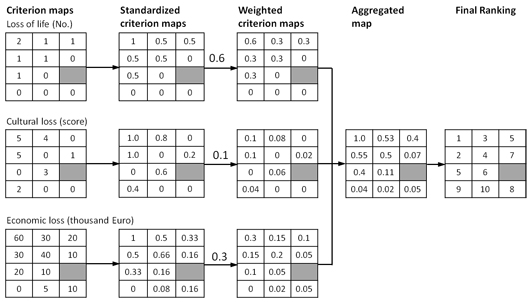
\includegraphics[width=\textwidth]{Figures/background/04_saw_method_web.jpg}
  \caption{SAW example \cite{SAWillustration}}
  \label{fig:SAW}
\end{figure}

\subsection{Weighted Product Method (WPM)}
This method is similar to SAW.
The main difference is that, instead of addition in the model, there is multiplication. The normalized values are calculated as explained under the SAW method \cite{WPM}. 

For example if we have the 3 alternatives each with 4 criteria as shown in
Table \ref{table:WPM_data}.
\begin{table}
\caption{Example alternatives \label{table:WPM_data}} 
\begin{center}
\begin{tabular}{ c c c c c }
\hline
&	Criteria1 &	Criteria2 &	Criteria3 &	Criteria4 \\
\hline
Weight &	0.20 &	0.15 &	0.40 &	0.25\\
\hline
Alternative1 &	25 &	20 &	15 &	30\\
Alternative2 &	10 &	30 &	20 &	30\\
Alternative3 &	30 &	10 &	30 &	10\\
\hline
\end{tabular}
\end{center}
\end{table}
WPM compare alternatives by computing a P value, like illustrated below:
$$
P(Alternative1/Alternative2)=
(\frac{25}{10})^{0.20}
*(\frac{20}{30})^{0.15}
*(\frac{15}{20})^{0.40}
*(\frac{30}{30})^{0.25}
=1.007 > 1
$$
Similarly, we also get:
$$
P(Alternative1/Alternative3)=1.067 > 1
$$
$$
P(Alternative2/Alternative3)=1.059 > 1
$$
Therefore, the best alternative is Alternative1, since it is superior to all the other alternatives. Furthermore, the following ranking of all three alternatives is as follows: A1 > A2 > A3.

It is worth noting that a useful way of choosing
between an additive score function and a multiplicative one is to consider
whether one is willing to keep giving up or trading off units of one attribute
in exchange for some units of the other attribute, at
a given fixed exchange rate, even to the point where
one has zero of the first attribute. 
If this is not acceptable to the decision maker, then the additive score
function is not appropriate. Likewise, if one does not
believe the exchange rate should stay the same however high or low the attributes levels, then again an additive score function is not suitable \cite{AddorMultiply}.
For example, the UNDP (United Nations Development Programme)
publishes an annual ranking of nations known as the
\href{http://hdr.undp.org}{Human Development Index},
which is very influential and is used by first world
nations to guide their aid allocations.
It is also used by pharmaceutical companies to decide which countries should receive discounted prices.
This index is an aggregate of three criteria: life expectancy, education, and gross national income per capita.
For many years the aggregation was carried out using additive weighting.
This was criticised because this assumed that the criteria were perfectly substitutable. Consequently, the UNDP chose to
change its methodology, and the index
is now calculated using a multiplicative scheme.

\subsection{Analytical Hierarchy Process (AHP)}
One of the most popular analytical techniques for
complex decision-making problems is the analytical hierarchy process \cite{MCDM}.
AHP decomposes a decision-making problem into a system of hierarchies of objectives, attributes and alternatives. An AHP hierarchy can have as many levels as needed to fully characterize a particular decision situation. A number of functional characteristics make AHP a useful methodology. These include the ability to handle decision situations involving subjective judgments, multiple decision makers and the ability to provide measures of consistency of preference. Designed to reflect the way people actually think, AHP continues to be the most highly regarded and widely used decision-making method. AHP can efficiently deal with tangible as well as non-tangible attributes, especially where the subjective judgments of different individuals constitute an important part of the decision process.

\subsubsection{The Revised Analytic Hierarchy Process}
Belton and Gear \cite{revisedAHP} propose a revised version
of the AHP model. They demonstrate that an inconsistency can occur when the AHP is used. A numerical example is presented that consists of three criteria and three alternatives. The indication of the best alternative changes when an identical alternative to one of the non-optimal alternatives are introduced now creating four alternatives. According to the authors, the root for that inconsistency is the fact that the relative values for each criterion sum up to one. Instead of having the relative values of the alternatives sum up to one, they propose to divide each relative value by the maximum value of the relative values.

For example, the original step normalise eigenvector into:
$$\begin{bmatrix}
\frac{1}{11} \\
\frac{9}{11} \\
\frac{1}{11}
\end{bmatrix}$$

The revised method would normalise those to:
$$\begin{bmatrix}
\frac{1}{9} \\
1 \\
\frac{1}{9}
\end{bmatrix}$$

\subsection{Technique for Order Preference by Similarity to Identical Solution (TOPSIS)}
This method is based on the concepts that the chosen alternative should have the shortest Euclidean distance from ideal solution and the farthest from negative ideal solution \cite{MCDM}. The ideal solution is a hypothetical solution for which all attribute values corresponds to the maximum attribute values comprising the satisfying solutions; the negative ideal solution is the hypothetical solution for which all attribute values corresponds to the minimum attribute values.
TOPSIS thus gives a solution that is not only closest to the hypothetically best, that is also the farthest from hypothetically worst.

TOPSIS can suffer from ranking abnormality \cite{SAWvsTOPSIS}.
Ranking abnormality means that the ranking of candidate networks changes when low ranking alternative is removed from the candidate list.

\subsection{Compromise Ranking method (VIKOR)}
The VIKOR method of compromise ranking determines a compromise solution, providing a maximum "group utility" for the majority and a minimum of an "individual regret" for the "opponent"\cite{VIKORformula} .

The MCDM problem is stated as follows: Determine the best (compromise) solution in multicriteria sense from the set of J feasible alternatives $A_{1}, A_{2}$ \textellipsis $A_{J}$, evaluated according to the set of n criterion functions. The input data are the elements $f_{ij}$ of the performance (decision) matrix, where $f_{ij}$ is the value of the i-th criterion function for the alternative $A_{j}$.

The VIKOR procedure has the following steps \cite{VIKOR_method_wiki}:
\begin{enumerate}
    \item Determine the best $f_{i}^{*}$ and the worst $f_{i}^{-}$ values of all criterion functions, i = 1,2,...,n; if the i-th function is benefit:
    $$f_{i}^{*} =  \max\limits_{j} f_{ij} , f_{i}^{-} = \min\limits_{j} f_{ij}$$
    If the i-th function is cost:
    $$f_{i}^{*} = \min\limits_{j} f_{ij} ,f_{i}^{-} = \max\limits_{j} f_{ij}$$
    \item Compute the values $S_{j}$ and $R_{j}$, j=1,2,...,J, by the relations: 
    
    Weighted and normalized Manhattan distance:
    $$S_{j}=\sum_{i=1}^{n} w_{i} \frac{f_{i}^{*} - f_{ij}}{f_{i}^{*} - f_{i}^{-}}$$
    Weighted and normalized Chebyshev distance:
    $$R_{j}=\max\limits_{i} w_{i} \frac{f_{i}^{*} - f_{ij}}{f_{i}^{*} - f_{i}^{-}}$$
    where $w_{i}$ are the weights of criteria, expressing their relative importance.
    \item Compute the values $Q_{j}$, j=1,2,…,J, by the relation
    $$Q_{j} = v \frac{S_{j}-S^{*}}{S^{-}-S^{*}} + (1-v)\frac{R_{j}-R^{*}}{R^{-}-R^{*}}$$
    where 
    $$ S^{*} = \min\limits_{j} S_{j},
    S^{-} = \max\limits_{j} S_{j} $$
    $$ R^{*} = \min\limits_{j} R_{j},
    R^{-} = \max\limits_{j} R_{j} $$
    and v is introduced as a weight for the strategy of maximum group utility, whereas 1-v is the weight of the individual regret.
    \item Rank the alternatives, sorting by the values S, R and Q, from the minimum value. The results are three ranking lists.
    \item Propose as a compromise solution the alternative A(1) which is the best ranked by the measure Q (minimum) if the following two conditions are satisfied:
    \begin{enumerate}
        \item C1: “Acceptable Advantage”: $Q(A_{2})-Q(A_{1}) >= DQ$
        where: $A_{2}$ is the alternative with second position in the ranking list by Q; $DQ = \frac{1}{J-1}$, J is the number of alternatives.
        \item C2: “Acceptable Stability in decision making”: The alternative $A_{1}$ must also be the best ranked by S or/and R. This compromise solution is stable within a decision making process, which could be the strategy of maximum group utility (when v > 0.5 is needed), or “by consensus” v about 0.5, or “with veto” v < 0.5).
    \end{enumerate}
    If one of the conditions is not satisfied, then a set of compromise solutions is proposed, which consists of:
    \begin{enumerate}
        \item Alternatives $A_{1}$ and $A_{2}$ if only the condition C2 is not satisfied, or
        \item Alternatives $A_{1},A_{2}$,...,$A_{M}$ if the condition C1 is not satisfied; $A_{M}$ is determined by the relation $Q(A_{M})-Q(A_{1}) < DQ$ for maximum M (the positions of these alternatives are “in closeness”).
    \end{enumerate}
\end{enumerate}

The obtained compromise solution could be accepted by the decision makers because it provides a maximum utility of the majority (represented by min S), and a minimum individual regret of the opponent (represented by min R). The measures S and R are integrated into Q for compromise solution, the base for an agreement established by mutual concessions.

\subsection{Preference Ranking Organization Method for Enrichment Evaluation (PROMETHEE)}
The Preference Ranking Organization METHod for Enrichment of Evaluations and its descriptive complement geometrical analysis for interactive aid are better known as the Promethee and Gaia methods \cite{Promethee}.
The descriptive approach, named Gaia, allows the decision maker to visualize the main features of a decision problem: he/she is able to easily identify conflicts or synergies between criteria, to identify clusters of actions and to highlight remarkable performances.
The prescriptive approach, named Promethee, provides the decision maker with both complete and partial rankings of the actions \cite{PROMETHEE_MLwiki}.

While it can be used by individuals working on straightforward decisions, the Promethee Gaia method is most useful where groups of people are working on complex problems, especially those with several multi-criteria, involving a lot of human perceptions and judgments, whose decisions have a long-term impact. It has unique advantages when important elements of the decision are difficult to quantify or compare, or where collaboration among departments or team members are constrained by their different specializations or perspectives.

\subsection{Decision-making paradox}
The decision-making paradox arises from the quest for determining reliable decision-making methods.
To find the best decision-making method a decision problem needs to be formulated, for which different decision-making methods are the alternatives. 
Since in the beginning it was assumed that the best method is not known, the problem of selecting the best method was solved by successively using different methods. The methods used in that study \cite{DecisionMakingParadox} were the weighted sum model (WSM), the weighted product model (WPM), and two variants of the analytic hierarchy process (AHP). It was found that when a method was used, say method X (which is one of the previous four methods), the conclusion was that another method was best (say, method Y). When method Y was used, then another method, say method Z, was suggested as being the best one, and so on.

The study \cite{DecisionMakingParadox} demonstrates that it is impossible to determine precisely the best decision-making method, for to do so one needs to use the best decision-making method! This problem of finding the best decision-making method always reaches a Decision-Making Paradox. However, the results of this study recommend that for most of the cases of different weights of the two evaluative criteria the revised AHP appears to be the best decision-making method of the four examined, while the original AHP, appears to be the most inaccurate one.


%----------------------------------------------------------------------------------------
%	Cloud Service Identification and Representation
%----------------------------------------------------------------------------------------

\chapter{Cloud Service Ontology}
\label{cha:cocoon}
IaaS providers include Amazon Web Services (AWS), Microsoft Azure, Google, Alibaba and others. They give users the option to deploy their application over a pool of virtually infinite services with practically no capital investment and with modest operating costs proportional to the actual use. Elasticity, cost benefits and abundance of resources motivate many organizations to migrate their enterprise applications (e.g. Content management system, Customer relationship management system and Enterprise resource planning system) to the Cloud. Although Cloud offers the opportunity to focus on revenue growth and innovation, decision makers (e.g., CIOs, scientists, developers, engineers, etc.) are faced with the complexity of choosing among private, public, and hybrid Cloud options and selecting the right service delivery and deployment model, see Section \ref{subsec:service_discovery}.

To address this IaaS service discovery problem
we present an OWL-based ontology, the Cloud Computing Ontology (CoCoOn)
that defines functional and non-functional concepts, attributes
and relations of infrastructure services.

From a service discovery point of view, the selection process on the IaaS layer is based on a finite set of functional (e.g. CPU type, memory size, location) and non-functional (costs, QoS, security) configuration properties that can be satisfied by multiple providers. Similarly, there is a service discovery problem associated with the SaaS and PaaS offerings. However, we are not considering these issues in this thesis.
In cloud computing, SaaS services are often developed
and provided by third party service providers who are different from the IaaS providers.
We focus on IaaS that is the underpinning layer
on which the PaaS services are hosted for creating SaaS applications.
As there are less studies in IaaS selection compare to SaaS selection,
which a lot of the Service Composition techniques are directly applicable.


Although popular search engines (e.g., Google, Bing, etc)
can point users to these provider web sites (blogs, wikis, etc.)
that describe laaS service offerings, they are not designed to
compare and reason about the relations among the different
types of Cloud services and their configurations. Service
description models and discovery mechanisms for
determining the similarity among Cloud infrastructure
services are needed to aid the user in the discovery and
selection of the most cost effective infrastructure service
meeting the user's functional and non-functional
requirements.

In this chapter, We identify and formalize the domain knowledge of multiple
configurations of infrastructure services. The core idea is to
formally capture the domain knowledge of services using
semantic Web languages like the Resource Description
Framework (RDF) and the Web Ontology Language (OWL).
The contributions are as the following:
Identification of the most important concepts and
relations of functional and non-functional
configuration parameters of infrastructure services
and their definition in an ontology;
Modeling of service descriptions published by
Cloud providers according to the developed
ontology. By doing so, we validate the
expressiveness of ontology against the most
commonly available infrastructure services
including Amazon, Microsoft Azure, GoGrid, etc.


\section{Common Approaches}
In relation to research problem described in Section \ref{subsec:service_discovery}, there are 3 common approaches for web services identification/publication: 
\begin{enumerate}
    \item Manually maintain directories by categorizing manually-submitted or collected information about Cloud services and providers, an example of such kind is Universal Description, Discovery and Integration (UDDI), which has failed to gain wide adoption.
    \item Use web crawling, and automatically create listings.
    \item Combine both, e.g. using manually-submitted URIs as seeds to generate indexes. The first approach is the only feasible solution at the moment. But extensive research and standardization efforts have been put into developing web information representation models, namely, RDF, the semantic web, and ontologies \cite{Al-Hamdani2003}.
\end{enumerate}

\section{CoCoOn 0.1.0}
\label{sec:cocoon0.1}
The initial version of CoCoOn defines the
domain model of the IaaS layer. This ontology facilitates the
description of Cloud infrastructure services; and through
mappings from provider descriptions, facilitates the
discovery of infrastructure services based on their
functionality.
The ontology is defined in the OWL \cite{OWL}.
To describe specific aspects of
Cloud computing, established domain classifications have
been used as a guiding reference
\cite{UnifiedOntologyCloudComputing}.
For the layering of the ontology on top of Web service models,
it draws inspiration and ideas from standard semantic Web service ontologies i.e.,
OWL-S \cite{BringingSemanticsToWebServicesOWL-S}
and WSMO \cite{WSMO}. Consequently, modelers can use the
grounding model and process model of OWL-S in
combination with the presented Cloud computing ontology
to succinctly express common infrastructure Cloud services.
We mapped the most prominent set of infrastructure services
(i.e. Amazon, Azure, GoGrid, Rackspace, etc.) to CoCoOn.
All common meta data fields in the ontology including
Organization, Author, First Name etc. are referenced through
standard Web Ontologies (i.e. FOAF \cite{FOAF} and
Dublin Core \cite{DublinCore}).

The first version of CoCoOn consists of two parts:
functional Cloud service configurations information
parameters; and non-functional service configuration
parameters. In the following sections, we detail on these two
parts. We also present parts of the ontology in a visual form
produced by the Cmap Ontology Editor tool \cite{CmapToolsOntologyEditor}.

\subsection{Functional Parameters}
The main concept to describe functional Cloud service
configurations in CoCoOn 0.1.0 is a CloudResource that can be of
one of the three types: Infrastructure-as-a-Service ,
Platform-as-a-Service or Software-as-a-Service.

Cloud services in the IaaS layer can be categorised into:
Compute, Network, and Storage services
(See Fig. \ref{fig:CoCoOn0.1CloudResource}).
Compute is the main concept for infrastructure services,
whereas Network and Storage are usually attached to a
Compute service (with exceptions, for example
NetworkStorage).
Due to page limit, a larger graph is made available online at
\href{https://cmapscloud.ihmc.us/viewer/cmap/1SB4SYXQ2-1NW70FR-1MMSKJ}{here}.
The previous model's graph was generated by Cmap \cite{cmap}. 

\begin{figure}
  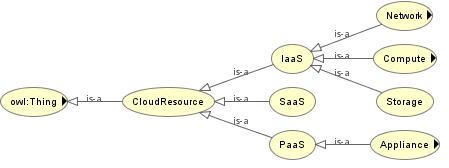
\includegraphics[width=\textwidth,keepaspectratio]{Figures/0.1/CloudResource.png}
  \caption{CoCoOn 0.1.0 Top Concepts in the IaaS layer}
  \label{fig:CoCoOn0.1CloudResource}
\end{figure}

The Compute class (see Fig. \ref{fig:CoCoOn0.1SubClassesPropertiesComputeStorageNetwork}) has the following object properties, hasVirtualization, hasCPU, hasMemoryAddressSize and hasNetworkStorage. The hasCPU property links a Compute unit to one or many processors which can be of type CPU or ClusteredCPU. A Compute object can be linked to a Storage object by using the top level object property hasStorage.

\begin{figure}
  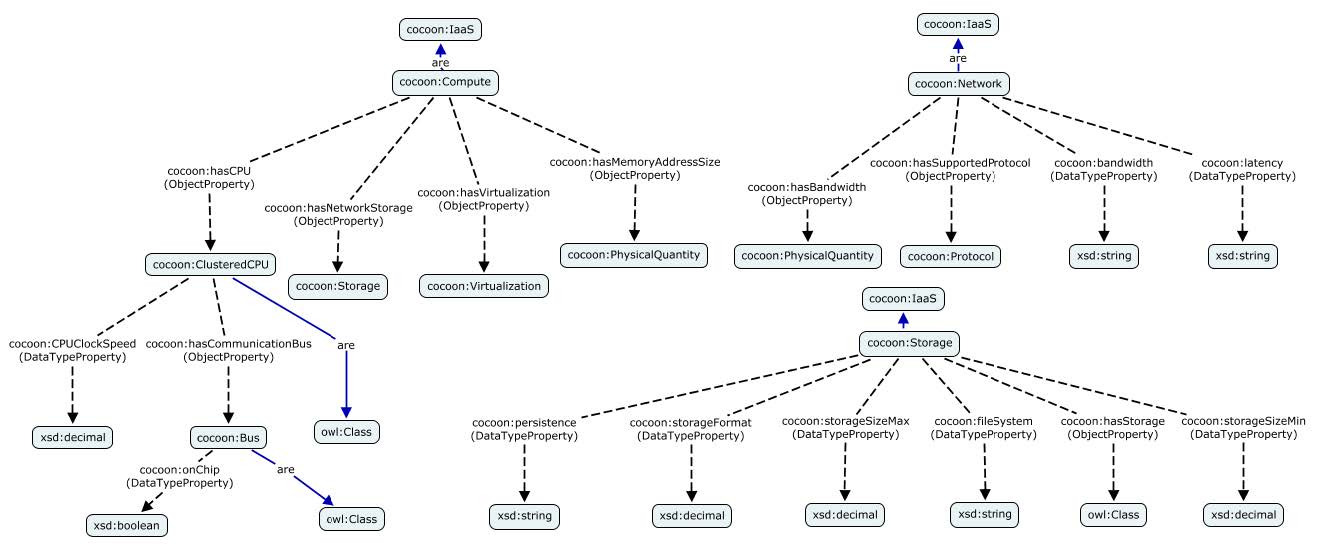
\includegraphics[width=\textwidth,keepaspectratio]
  {Figures/0.1/SubClassesPropertiesComputeStorageNetwork.jpg}
  \caption{CoCoOn 0.1.0 SubClasses and properties for the Compute, Storage and Network class}
  \label{fig:CoCoOn0.1SubClassesPropertiesComputeStorageNetwork}
\end{figure}

There are two different Storage types for a CloudResource: LocalStorage attached to a CPU with the hasLocalStorage property and NetworkStorage attached to a Compute instance with the hasNetworkStorage property. The hasNetworkStorage is an \textit{owl:inverseOf} property of the isAttached property which can be used to define that a Storage resource is attached to a Compute resource. There is also an important distinction to be made between Storage resources that \underline{are} attached to a Compute resource and Storage resources that \underline{can be} attached. The latter is modeled with the \textit{isAttachable} object property and its inverse property \textit{hasAttachable}. These relations are important for the discovery of infrastructure services based on a user requirement.
For example, in the case of Amazon, we can model that a \textit{BlockStorage} with a \textit{StorageSizeMin} of 1GB and a \textit{StorageSizeMax} of 1TB can be attached to any EC2 Compute resource instance i.e., Standard, Micro, High-Memory, High-CPUCluster, ComputeCluster, GPUHigh-I/O.
Consequently, if a user searches for a specific Compute instance with, for example, 5GB persistent storage, the relevant EC2 Compute resource and an Amazon BlockStorage will be returned (possibly among others). That is, because the isAttached relation in the user request can be matched with the definition of the Amazon EC2 unit with a BlockStorage defined to be isAttachable.

A Network resource can be described with the
has Bandwidth and hasProtocol properties. Similarly, to how
Storage resources are attached to Compute resource, we
distinguish between the hasSupportedNetwork and
hasNetwork property to either express that the specific
network types can be used with a Compute resource or that
they are in fact used.

\subsection{Non-Functional Parameters}
For non-functional Cloud service configuration parameters we distinguish between non-functional properties and QoS attributes. The first are properties of Cloud resources that are known at design time, for example,
PriceStorage, Provider, DeploymentModel,
whereas QoS attributes can only be recorded after at least one execution cycle of a Cloud service, for example, DiskReadOperations, Networkln, NetworkOut etc.
For QoS attributes, we distinguish MeasurableAttributes like the ones above and
UnmeasurableAttributes like Durability or Performance.

The QoS attributes define a taxonomy of Attributes and Metrics,
i.e. two trees formed using the \textit{rdfs:subClassOf} relation where
a ConfigurationParameter, for example, PriceStorage, PriceCompute, PriceDataTransferIn (Out) etc;
and a Metric, for example, ProbabilityOfFailureOnDemand, TransactionalThroughput, are used in combination to
define non-functional properties (e.g. Performance, Cost, etc.). The resulting ontology is a directed graph where, for example,
the Property hasMetric (and its inverse isMetricOf) is the basic link between ConfigurationParameters and \textit{Metric} trees. For the
QoS metrics, we used existing QoS ontologies \cite{QoSOnt} as a reference whereas
for the ConfigurationParameters concepts the ontology defines its independent taxonomy, but refer to external ontologies for existing definitions
(e.g. QUDT \cite{QUDT}). Each configuration
parameter has a \textit{Name} and a \textit{Metric} (qualitative or quantitative).
The \textit{Metric} itself has UnitOfMeasurement and Value. The type of configuration determines the nature of a service by means of setting a minimum, maximum, or capacity limit, or meeting a certain value. For example, the hasMemory configuration parameter
of a Compute service can be set to have a Value of 2 and a UnitOfMeasurement of GB.

\section{CoCoOn 1.0.1}
\label{sec:cocoon1.0.1}
As the Web brings people into an age of information overload,
presenting only most relevant personalized and reliable
information to customers is crucial to business success.
Consumers of Cloud computing services also need better recommendation
for them to make informed decisions.
To fulfill the goal of a smart Cloud service recommendation,
an unified model is needed as foundation for data collection reasoning and analytics.
Due to the Cloud's relative new emergence compared to traditional Computer Science fields, there is a lack of a well recognized standard ontology model.
Semantic technologies are commonly employed to build such a model.
Since there are other models that focus on such a model for Services and Web Services in general, our model only focuses on Cloud computing Infrastructure as a Services (IaaS) aspects like features and prices.

The ontology can be accessed online via:
\url{https://w3id.org/cocoon/v1.0.1}

\subsection{Major Change}
We have proposed a simpler model describing concepts of Cloud infrastructure services (IaaS)
in our previous work \cite{IJNGC2013,CoCoOn2012},
see Section \ref{sec:cocoon0.1}. This work was mostly a taxonomy of IaaS.
In this section we will propose an extension focusing on the core parameters for comparing and recommending IaaS services.

We also aware of the popularity of schema.org, and hence made this version compatible with its vocabularies and hope CoCoOn can become an extension to schema.org, as there is no existing definition covered the Cloud service domain. During this process we observed that despite schema.org's wide deployments among websites, it is not defined with OWL2 semantics, which has the most expressive power (in comparison to RDF).

We revised our CoCoOn ontology, i.e. changes have been made to namespaces, classes, properties, relationships and axioms, with a strong focus on flexibility and extensibility.

We also introduced versioning from this release, for both ontology and data, following the
\href{https://semver.org/}{semantic versioning specification}. Although this ontology is not in a sense of "in production",
this version is a stable release that we are intended to keep long term support and availability. We label the collection date of data with \schema{dateModified}, thus historical price data can be recorded.

The new model is outlined in Section \ref{sec:CoCoOnextended},
with explanation of its syntax and semantics, design, formalization.

It has been a long time since we proposed the initial model of CoCoOn, which we retrospectively versioned 0.1.0, hence there are many advances in both the Semantic Web field and Cloud Computing.
The major model changes are summarized below:
\begin{enumerate}
  \item Additional external vocabularies.
  \item Additional annotations, including version number, modification dates, metadata like author,
  web page etc.
  \item Removed classes and properties which are not core, and possibly covered by some other ontologies, e.g. Input, Output, Interface, User.
  \item New class and properties focusing on IaaS and price specifications. Like \cocoon{OSPriceSpecification} and various other extensions to \gr{UnitPriceSpecification}; subclasses for specific Cloud features i.e. \cocoon{LoadBalancing}; classes for describing properties like \cocoon{TrafficDirection}, which specifies network data flow direction.
\end{enumerate}
A detailed change log can also be find on the online documentation 
\href{https://w3id.org/cocoon/v1.0.1#changes}{"Changes from last version" section}.

On top of that we developed a full mapping service between CoCoOn 1.0.1, and Cloud vendor APIs for the Google Cloud and the Microsoft Azure Cloud.
These mapping services demonstrates the usability and strength of the ontology developed. More details can be found in Section \ref{sec:cocoonImplementation}.

We also used existing ontologies whenever fits, such as 
the Unit of Measure Ontology (QUDT) \cite{OntologyUnitsOfMeasure} for defining price with currency values, see Section \ref{sec:ReusingExistingVocabularies} for more details.

\subsection{Reusing Existing Vocabularies}
\label{sec:ReusingExistingVocabularies}
A set of well-known vocabularies has evolved in the Semantic Web community.
The set of established vocabularies we reuse are listed in Table \ref{table:namespaces}.

\begin{longtable}[ht]{ p{.15\textwidth} p{.35\textwidth} |p{.15\textwidth} p{.25\textwidth} }
\hline
Names & Details & Namespaces & URIs \\ \hline
OWL2 & Web Ontology Language Schema 2. & owl & \url{http://www.w3.org/2002/07/owl\#} \\ \hline
RDF & Resource Description Framework Concepts Vocabulary. & rdf & \url{http://www.w3.org/1999/02/22-rdf-syntax-ns\#}\\
& RDF Schema vocabulary. & rdfs & \url{http://www.w3.org/2000/01/rdf-schema\#} \\
\hline
XML Schema Definition & Data types for elements and attributes. & xsd & \url{http://www.w3.org/2001/XMLSchema\#} \\ \hline
DCMI Metadata Terms & Defines general metadata attributes & dcterms & \url{http://purl.org/dc/terms/}\\ \hline
VANN & Vocabulary for annotating descriptions of vocabularies with examples and usage notes. & vann & \url{http://purl.org/vocab/vann/} \\ \hline
Friend of a Friend & People and relationship. & foaf & \url{http://xmlns.com/foaf/0.1/} \\ \hline
Creative Commons & License terms. & cc & \url{http://creativecommons.org/ns\#}  \\ \hline
Geo Names & Geographic places. & gn & \url{http://www.geonames.org/ontology\#} \\ \hline
Schema.org & Vocabulary for common concepts, i.e. TypeAndQuantityNode, GeoCoordinates, e.t.c. & schema & \url{https://schema.org/} \\ \hline
Good Relations & Product, price and company data. & gr & \url{http://purl.org/goodrelations/v1\#} \\\hline
QUDT & Units and measurements schema. & qudt & \url{http://qudt.org/schema/qudt\#}\\ 
& Unit vocabulary. & unit & \url{http://qudt.org/vocab/unit\#}\\
\hline
Semantic Sensor Network & SSN is an ontology for describing sensors and their observations, the studied features of interest, the samples used to do so, and the observed properties. & ssn & \url{http://www.w3.org/ns/ssn/}\\
& System capabilities terms of SSN ontology. & ssn-system & \url{http://www.w3.org/ns/ssn/systems/}\\
& Sample Observation and Actuator. & sosa & \url{http://www.w3.org/ns/sosa/}\\
\hline
\caption{Vocabularies}
\label{table:namespaces}
\end{longtable}

We have also considered a number of other vocabularies, but decided they are not suitable for our case:
\begin{enumerate}
  \item OWL-S \cite{OWL-S}: It is more useful when defining the input, output and interactions between web services, but CoCoOn is not modeling those.
  \item Unified Code for Units of Measure (UCUM) \cite{UCUM} and Custom Datatypes \cite{CDT}: These ontologies do not include the units needed for our use case, see Section \ref{sec:unit}.
\end{enumerate}

\subsection{Concepts and Design}
\label{sec:CoCoOnextended}
The relevant code and ontology itself is made available online at this
\href{https://github.com/miranda-zhang/cloud-computing-schema}{Github project page}.

In this section we describe the main conceptual components of CoCoOn 1.0.1,
how they evolved, the rationale behind their design and some example usages.
The examples are in Turtle syntax \cite{turtle}. 
The class expressions are in
\href{http://protegeproject.github.io/protege/class-expression-syntax/}{Manchester OWL Syntax}
\cite{ManchesterOWLSyntax},
which is what Protege \cite{Protege} use.
We will show the prefix definitions once,
then omit the duplicated definitions in the following examples.

The specification of the models suggests the arrangement of classes and properties according to subsumption hierarchies
(OWL uses the \rdfs{subClassOf} for representing subsumption),
which represent the skeleton of the model and establish the basic relationships between the components.

Following the principle of minimal commitment \cite{principles_for_minimal_commitments},
we use guarded restriction (i.e., existential quantifier, $\exists$,
\magenta{some}, \owl{someValuesFrom})
instead of domain range restrictions (\rdfs{domain}, \rdfs{range}).
As such, the domain and ranges are more permissive,
keeping the model more flexible.
We also use qualified cardinality restrictions
(e.g., \magenta{exactly}, \owl{qualifiedCardinality};
\magenta{max}, \owl{maxQualifiedCardinality}) when there
is a known cardinality restriction.

\subsubsection{Cloud Service Feature}
Most building blocks of IaaS services naturally correspond to OWL2 classes 
(e.g., \cocoon{CloudService}, \cocoon{ComputeService}, \cocoon{StorageService}), object properties (e.g., \cocoon{hasMemory}, \cocoon{hasStorage}, \cocoon{inRegion})
and data properties (e.g., \cocoon{numberOfCores}).
The more challenging part is to capture constraints posed by the possible combination of services in IaaS in the models using ontological axioms.
We next describe how this was accomplished using a combination of OWL2 axioms and integrity constraints.

\subsubsubsection{Cloud Service}
The class \cocoon{CloudService} is the main class hosting our Cloud feature vocabularies.
We defined a top level class \cocoon{Service} to be its parent, and make it the union of \schema{Service} and \sosa{FeatureOfInterest}.
So our Cloud service definitions are compatible with schema.org and SOSA ontology.
As later we need to use vocabularies from both.

Cloud Services are usually classified into three categories:
\cocoon{IaaS}, \cocoon{PaaS}, \cocoon{SaaS}.
We focus on modelling IaaS, see Section \ref{sec:IaaS} for more details.
We have classified \cocoon{SystemImage} as a subclass of \cocoon{SaaS},
as a computer system is like any other software, and can be installed on different compatible hardware.
Some examples of \cocoon{SaaS} are database as a service, machine learning as a service, Google Cloud Composer, etc.
Some examples of \cocoon{PaaS} are Google App Engine, Heroku, etc.

The following properties are defined for the class \cocoon{CloudService}:
\begin{itemize}
    \item[] \gr{hasPriceSpecification} \magenta{some} \gr{UnitPriceSpecification}
    \item[] \cocoon{hasProvider} \magenta{exactly} 1 \gr{BusinessEntity}
    \item[] \cocoon{inRegion} \magenta{exactly} 1 \cocoon{Region}
    \item[] \cocoon{inZone} \magenta{max} 1 \xsd{string}
\end{itemize}

We use \gr{UnitPriceSpecification} and its associated object property \gr{hasPriceSpecification}
to model price, see Section \ref{sec:PriceSpecification} for more details about price specification.
Existential quantifiers (i.e., \magenta{some}, \owl{someValuesFrom}) are used on \gr{hasPriceSpecification}.

Note that, \magenta{some} is the same as \magenta{min} 1. 
But this is not the same as database integrity constrains.
We can still define (Cloud service) individuals without a price specification.
Under the open world assumption, missing information is just not known but may exist, whereas in databases (closed world assumption), absence of information often assumes that the information does not exist.
We can not guarantee all services will have a price specification, as there are services available upon request, but the price is negotiated later. For example, we may want to specify that secure data centers for governmental use
are available, but detailed information is probably not disclosed publicly.

We assume each service can belong to exactly one provider.
A qualified cardinality restriction \magenta{exactly} (\owl{qualifiedCardinality}) is used to define this type of assumption.
We used \gr{BusinessEntity} to describe a provider, see Section \ref{sec:Provider} for more details.

\subsubsubsection{Infrastructure as a Service}
\label{sec:IaaS}
Infrastructure as a Service can be classified into 3 categories:
\cocoon{ComputeService} (see Section \ref{sec:VM}),
\cocoon{StorageService} (see Section \ref{sec:Storage}),
\cocoon{NetworkService} (see Section \ref{sec:Network}).

\subsubsubsection{Compute Service}
\label{sec:VM}
We define the following properties for class \cocoon{ComputeService}:
\begin{itemize}
  \item[] \cocoon{numberOfCores} \magenta{max} 1 \xsd{decimal}
  \item[] \cocoon{hasCPUcapacity} \magenta{max} 1 \schema{TypeAndQuantityNode}
  \item[] \cocoon{hasMemory} \magenta{exactly} 1 \schema{TypeAndQuantityNode}
  \item[] \cocoon{hasStorage} \magenta{max} 1 \schema{TypeAndQuantityNode}
  \item[] \cocoon{hasMaxStorageSize} \magenta{max} 1 \schema{TypeAndQuantityNode}
  \item[] \cocoon{hasMaxNumberOfDisk} \magenta{max} 1 \schema{TypeAndQuantityNode}
  \item[] \gr{hasPriceSpecification} \magenta{max} 1 \cocoon{CloudStorageTransactionsPriceSpecification}
\end{itemize}

The number of cores available on a virtual machine(VM) is defined by the data property \cocoon{numberOfCores}.
Because it can have non integer value, we made it accept \xsd{decimal}.
For Google Cloud, cores and vCPU refer to the same thing.

\cocoon{hasCPUcapacity} is used to describe the performance power of the CPU.

The memory size of a VM is specified by \cocoon{hasMemory}.

The \cocoon{LocalStorage} available on a VM can be specified with \cocoon{hasStorage}.
We quantify this object property with \magenta{some}, so that it is possible to define more \cocoon{NetworkStorage} later.
Google has a limit for the maximum number of disks that can be attached to a VM, which we model with the object property \cocoon{hasMaxNumberOfDisk}.
Additionally, Google also has a limit for the maximum total disk size that can be attached to a VM, which is modelled with \cocoon{hasMaxStorageSize}.

We use \schema{TypeAndQuantityNode} to describe some quantity of things.
So value, unit, and the type of the object can all be captured. See Section \ref{sec:TypeAndQuantityNode} for more examples.

Note that this class also inherits properties from its super classes, e.g. the property inherited from \cocoon{CloudService}:

\gr{hasPriceSpecification} \magenta{some} \gr{UnitPriceSpecification}

We provids a short example of \cocoon{ComputeService} in Listing \ref{lst:VM}.

There are data access fees on local disk of the Azure VM \cite{data_access_fees_local_disk_AzureVM}. To model this we use
\gr{hasPriceSpecification} \magenta{max} 1 \cocoon{StorageTransactionsPriceSpecification}.
See Section \ref{sec:StorageTransactionsPriceSpecification} for an example.

\begin{lstlisting}[caption={Virtual Machine},label={lst:VM}]
@prefix schema: <https://schema.org/> .
@prefix unit:  <http://qudt.org/vocab/unit#> .
@prefix xsd:   <http://www.w3.org/2001/XMLSchema#> .
@prefix rdfs:  <http://www.w3.org/2000/01/rdf-schema#> .
@prefix gr:    <http://purl.org/goodrelations/v1#> .
@prefix cocoon: <https://w3id.org/cocoon/v1.0.1#> .
@base <https://w3id.org/cocoon/data/v1.0.1/> .
<2019-02-12/ComputeService/Gcloud/CP-COMPUTEENGINE-VMIMAGE-N1-HIGHCPU-96-PREEMPTIBLE>
        a                         cocoon:ComputeService ;
        rdfs:label                "CP-COMPUTEENGINE-VMIMAGE-N1-HIGHCPU-96-PREEMPTIBLE" ;
        gr:hasPriceSpecification  [ a                        cocoon:CloudServicePriceSpecification ;
                                    gr:hasCurrency           "USD" ;
                                    gr:hasCurrencyValue      "0.72"^^xsd:float ;
                                    gr:hasUnitOfMeasurement  unit:Hour ;
                                    cocoon:inRegion         <Region/Gcloud/us-east1>
                                  ] ;
        cocoon:hasMemory          [ a                        schema:TypeAndQuantityNode ;
                                    schema:amountOfThisGood  86.4 ;
                                    schema:unitCode          cocoon:GB
                                  ] ;
        cocoon:hasProvider        cocoon:Gcloud ;
        cocoon:numberOfCores      "96"^^xsd:decimal ;
        schema:dateModified       "2019-02-12"^^xsd:date .
<2019-03-07/ComputeService/Azure/windows-m128-64ms-standard>
        a                         cocoon:ComputeService ;
        rdfs:label                "windows-m128-64ms-standard" ;
        gr:hasPriceSpecification  <2019-03-07/CloudStorageTransactionsPriceSpecification/Azure/vm_base> ;
        gr:hasPriceSpecification  [ a                        cocoon:CloudServicePriceSpecification ;
                                    gr:hasCurrency           "USD" ;
                                    gr:hasCurrencyValue      "47.827e0"^^xsd:float ;
                                    gr:hasUnitOfMeasurement  unit:Hour ;
                                    cocoon:inRegion         <Region/Azure/japan-east>
                                  ] ;
        cocoon:hasMemory          [ a                        schema:TypeAndQuantityNode ;
                                    schema:amountOfThisGood  "3800"^^xsd:decimal ;
                                    schema:unitCode          cocoon:GB
                                  ] ;
        cocoon:hasProvider        cocoon:Azure ;
        cocoon:hasStorage         [ a                        schema:TypeAndQuantityNode ;
                                    schema:amountOfThisGood  "4096"^^xsd:decimal ;
                                    schema:typeOfGood        cocoon:LocalStorage ;
                                    schema:unitCode          cocoon:GB
                                  ] ;
        cocoon:numberOfCores      "64"^^xsd:decimal ;
        schema:dateModified       "2019-03-07"^^xsd:date .
\end{lstlisting}

\subsubsubsection{Storage Service}
\label{sec:Storage}
We define the following properties for the class \cocoon{StorageService}:
\begin{itemize}
  \item[] \cocoon{canHaveSnapshot} \magenta{some} \cocoon{StorageService}
  \item[] \cocoon{hasStorageIOMax} \magenta{max} 1 \schema{TypeAndQuantityNode}
  \item[] \cocoon{hasStorageSize} \magenta{max} 1 \schema{TypeAndQuantityNode}
  \item[] \cocoon{hasStorageThroughputMax} \magenta{max} 1 \schema{TypeAndQuantityNode}
\end{itemize}
Two subclasses of storage services have been defined: \cocoon{LocalStorage} and \cocoon{NetworkStorage}.

On Azure Cloud, snapshots options are available for storage, which is modeled with
the object property \cocoon{canHaveSnapshot}. This information is 
\href{https://github.com/miranda-zhang/cloud-computing-schema/blob/master/example/azure/storage.md#disk-snapshots}{manually interpreted from the documentation}.
There are also caps on input/output operations per sec (IOPS) and throughput, which are modeled with
\cocoon{hasStorageIOMax} and \cocoon{hasStorageThroughputMax}. We have also defined corresponding units, see Section \ref{sec:unit}.

In example Listing \ref{lst:Storage}, we have show a \cocoon{NetworkStorage} service from \cocoon{Azure}, which is a Cloud provider we have pre-defined as a named instance.
For more details on its corresponding Storage Transactions Prices,
see Section \ref{sec:StorageTransactionsPriceSpecification}.
Followed this we have given an example of snapshot service with only some of the regions shown. Next, the Azure provisional Ultra SSD storage service. It has configurable IOPS and throughput, and price are based on provisioned storage size, IOPS and throughput.This is also a reservation charge imposed if you enable Ultra SSD capability on the VM without connecting an Ultra SSD disk, which is rate at per vcpu/hour provisioned.

\begin{lstlisting}[caption={Storage},label={lst:Storage}]
@base <https://w3id.org/cocoon/data/v1.0.1/> .
<2019-03-07/NetworkStorage/Azure/premiumssd-p30>
        a                               cocoon:NetworkStorage ;
        rdfs:label                      "premiumssd-p30" ;
        gr:hasPriceSpecification        <CloudStorageTransactionsPriceSpecification/Azure/managed_disk/transactions-ssd> ;
        gr:hasPriceSpecification        [ a                        gr:CloudServicePriceSpecification ;
                                          gr:hasCurrency           "USD" ;
                                          gr:hasCurrencyValue      "135.17e0"^^xsd:float ;
                                          gr:hasUnitOfMeasurement  cocoon:GBPerMonth ;
                                          cocoon:inRegion         <Region/Azure/australia-east>
                                        ] ;
        cocoon:canHaveSnapshot          <NetworkStorage/Azure/standardssd-snapshot> , <NetworkStorage/Azure/standardhdd-snapshot-zrs> , <NetworkStorage/Azure/premiumssd-snapshot> , </NetworkStorage/Azure/standardhdd-snapshot-lrs> ;
        cocoon:hasProvider              cocoon:Azure ;
        cocoon:hasStorageIOMax          [ a                        schema:TypeAndQuantityNode ;
                                          schema:amountOfThisGood  "5000"^^xsd:nonNegativeInteger ;
                                          schema:unitCode          cocoon:IOPs
                                        ] ;
        cocoon:hasStorageSize           [ a                        schema:TypeAndQuantityNode ;
                                          schema:amountOfThisGood  "1024"^^xsd:nonNegativeInteger ;
                                          schema:unitCode          cocoon:GB
                                        ] ;
        cocoon:hasStorageThroughputMax  [ a                        schema:TypeAndQuantityNode ;
                                          schema:amountOfThisGood  "200"^^xsd:nonNegativeInteger ;
                                          schema:unitCode          unit:MegabitsPerSecond
                                        ].
<2019-03-07/NetworkStorage/Azure/standardssd-snapshot>
        a                         cocoon:NetworkStorage ;
        rdfs:label                "standardssd-snapshot" ;
        gr:hasPriceSpecification  [ a                        gr:CloudServicePriceSpecification ;
                                    gr:hasCurrency           "USD" ;
                                    gr:hasCurrencyValue      "0.1188e0"^^xsd:float ;
                                    gr:hasUnitOfMeasurement  cocoon:GBPerMonth ;
                                    cocoon:inRegion         <Region/Azure/south-india>
                                  ] ;
        gr:hasPriceSpecification  [ a                        gr:CloudServicePriceSpecification ;
                                    gr:hasCurrency           "USD" ;
                                    gr:hasCurrencyValue      "0.132e0"^^xsd:float ;
                                    gr:hasUnitOfMeasurement  cocoon:GBPerMonth ;
                                    cocoon:inRegion         <Region/Azure/canada-east>
                                  ] .
<2019-03-07/NetworkStorage/Azure/ultrassd>
        a                         cocoon:NetworkStorage ;
        rdfs:label                "ultrassd" ;
        gr:hasPriceSpecification  [ a                        gr:CloudServicePriceSpecification ;
                                    rdfs:label               "stored" ;
                                    gr:hasCurrency           "USD" ;
                                    gr:hasCurrencyValue      "8.2E-5"^^xsd:float ;
                                    gr:hasUnitOfMeasurement  cocoon:GBPerHour ;
                                    cocoon:inRegion         <Region/Azure/us-east-2>
                                  ] ;
        gr:hasPriceSpecification  [ a                        gr:CloudServicePriceSpecification ;
                                    rdfs:label               "iops" ;
                                    gr:hasCurrency           "USD" ;
                                    gr:hasCurrencyValue      "3.4E-5"^^xsd:float ;
                                    gr:hasUnitOfMeasurement  cocoon:IOPsPerHour ;
                                    cocoon:inRegion         <Region/Azure/us-east-2>
                                  ] ;
        gr:hasPriceSpecification  [ a                        gr:CloudServicePriceSpecification ;
                                    rdfs:label               "throughput" ;
                                    gr:hasCurrency           "USD" ;
                                    gr:hasCurrencyValue      "6.85E-4"^^xsd:float ;
                                    gr:hasUnitOfMeasurement  cocoon:MegabitsPerSecondPerHour ;
                                    cocoon:inRegion         <Region/Azure/us-east-2>
                                  ] ;
        gr:hasPriceSpecification  [ a                        gr:CloudServicePriceSpecification ;
                                    rdfs:label               "vcpu" ;
                                    gr:hasCurrency           "USD" ;
                                    gr:hasCurrencyValue      "0.003e0"^^xsd:float ;
                                    gr:hasUnitOfMeasurement  cocoon:VcpuPerHour ;
                                    cocoon:inRegion         <https://w3id.org/cocoon/data/v1.0.1/Region/Azure/us-east-2>
                                  ] .
<2019-02-12/NetworkStorage/Gcloud/CP-COMPUTEENGINE-STORAGE-PD-SSD-REGIONAL>
        a                         cocoon:NetworkStorage ;
        rdfs:label                "CP-COMPUTEENGINE-STORAGE-PD-SSD-REGIONAL" ;
        gr:hasPriceSpecification  [ a                        gr:CloudServicePriceSpecification ;
                                    gr:hasCurrency           "USD" ;
                                    gr:hasCurrencyValue      "0.29"^^xsd:double ;
                                    gr:hasUnitOfMeasurement  cocoon:GBPerMonth ;
                                    cocoon:inRegion         <Region/Gcloud/asia-south1>
                                  ] ;
        cocoon:hasProvider        cocoon:Gcloud ;
        schema:dateModified       "2019-02-12"^^xsd:date .
\end{lstlisting}

\subsubsubsection{Network Service}
\label{sec:Network}
We classify network services into the following categories:
\cocoon{InternetService}, \cocoon{LoadBalancing}, \cocoon{StaticIPService} and \cocoon{DNSService}.

\paragraph{Internet Service}
\label{sec:Internet}
We define the following properties for the class \cocoon{InternetService}:
\begin{itemize}
  \item[] \cocoon{hasDirection} \magenta{exactly} 1 \cocoon{TrafficDirection}
  \item[] \cocoon{hasDestination} \magenta{some} \cocoon{Location}
  \item[] \cocoon{excludesDestination} \magenta{some} \cocoon{Location}
\end{itemize}
There is generally no charge to ingress traffic,
unless there is a load balancer used.
We use the \cocoon{hasDirection} object property to indicate the direction of traffic.
A class \cocoon{TrafficDirection} is also constructed with 2 disjoint subclasses:
\cocoon{Egress} and \cocoon{Ingress}. Those can be used to indicate the direction of traffic.

Internet egress rates are based on usage and destination.
For example, Google Cloud has the following destination categories:
Australia, China (excluding Hong Kong) and
Worldwide (excluding China and Australia, but including Hong Kong).
In this case, the object properties \cocoon{hasDestination} and \cocoon{excludesDestination} can be used to specify destination ranges.
Because traffic destinations are not constrained by cloud service regions,
\cocoon{Location} is used, see Section \ref{sec:Region} for more details.

The internet egress traffic prices can be modeled by \cocoon{CloudNetworkPriceSpecification}, see Section \ref{sec:NetworkPriceSpecification} for more details.

Listing \ref{lst:GoogleCloudNetworkPriceWorldwide} shows an example for Google Cloud Internet Service Prices.

\begin{lstlisting}[caption={Google Cloud Network Price Example: Worldwide Egress},label={lst:GoogleCloudNetworkPriceWorldwide}]
@base <https://w3id.org/cocoon/data/v1.0.1/2019-02-12/> .
<InternetService/Gcloud/CP-COMPUTEENGINE-INTERNET-EGRESS-NA-NA>
        a                           cocoon:InternetService ;
        rdfs:label                  "CP-COMPUTEENGINE-INTERNET-EGRESS-NA-NA" ;
        gr:hasPriceSpecification    [ a                         cocoon:CloudNetworkPriceSpecification ;
                                      gr:hasCurrency            "USD" ;
                                      gr:hasCurrencyValue       "0.11"^^xsd:float ;
                                      gr:hasUnitOfMeasurement   cocoon:GBPerMonth ;
                                      cocoon:forUsageLessEqual  cocoon:10TB ;
                                      cocoon:forUsageMoreThan   cocoon:1TB
                                    ] ;
        gr:hasPriceSpecification    [ a                         cocoon:CloudNetworkPriceSpecification ;
                                      gr:hasCurrency            "USD" ;
                                      gr:hasCurrencyValue       "0.08"^^xsd:float ;
                                      gr:hasUnitOfMeasurement   cocoon:GBPerMonth ;
                                      cocoon:forUsageLessEqual  cocoon:90TB ;
                                      cocoon:forUsageMoreThan   cocoon:10TB
                                    ] ;
        gr:hasPriceSpecification    [ a                         cocoon:CloudNetworkPriceSpecification ;
                                      gr:hasCurrency            "USD" ;
                                      gr:hasCurrencyValue       "0.12"^^xsd:float ;
                                      gr:hasUnitOfMeasurement   cocoon:GBPerMonth ;
                                      cocoon:forUsageLessEqual  cocoon:1TB ;
                                      cocoon:forUsageMoreThan   [ a                        schema:TypeAndQuantityNode ;
                                                                  schema:amountOfThisGood  "0"^^xsd:nonNegativeInteger ;
                                                                  schema:unitCode          cocoon:GB
                                                                ]
                                    ] ;
        cocoon:excludesDestination  <Location/China> , <Location/Australia> ;
        cocoon:hasDestination       <Location/Worldwide> , <Hong%20Kong> ;
        cocoon:hasDirection         cocoon:Egress ;
        cocoon:hasProvider          cocoon:Gcloud ;
        schema:dateModified         "2019-02-12"^^xsd:date .
\end{lstlisting}

\paragraph{Load Balancing}
\label{sec:LoadBalancing}
Both hardware and software-based load balancing solutions exist. 
Here we consider load balancing as a hardware feature, unless it is known otherwise.
We create a class \cocoon{LoadBalancing} to represent such a service.
It is further broken down into 2 subclasses: \cocoon{LoadBalancingData} and
\cocoon{ForwardingRule}.

Ingress data processed by a load balancer is charged (Per GB) based on region.
Listing \ref{lst:LoadBalancingDataPriceSpecification} shows an example modelling such case with \cocoon{LoadBalancingData}.
\begin{lstlisting}[caption={Load Balancing Data Price Specification},label={lst:LoadBalancingDataPriceSpecification}]
@base <https://w3id.org/cocoon/data/v1.0.1/2019-02-12/> .
<LoadBalancingData/Gcloud>
        a                         cocoon:LoadBalancingData ;
        gr:hasPriceSpecification  [ a                        gr:CloudServicePriceSpecification ;
                                    gr:hasCurrency           "USD" ;
                                    gr:hasCurrencyValue      "0.008e0"^^xsd:float ;
                                    gr:hasUnitOfMeasurement  cocoon:GB ;
                                    cocoon:inRegion         <Region/Gcloud/us>
                                  ] ;
        gr:hasPriceSpecification  [ a                        gr:CloudServicePriceSpecification ;
                                    gr:hasCurrency           "USD" ;
                                    gr:hasCurrencyValue      "0.009e0"^^xsd:float ;
                                    gr:hasUnitOfMeasurement  cocoon:GB ;
                                    cocoon:inRegion         <Region/Gcloud/europe-west4>
                                  ] ;
        cocoon:hasDirection       cocoon:Ingress ;
        cocoon:hasProvider        cocoon:Gcloud ;
        schema:dateModified       "2019-02-12"^^xsd:date .
\end{lstlisting}

Forwarding rules that are created for load balancing are also charged.
This can be modelled by \cocoon{ForwardingRule}.
For example, pricing for rules on the Google Cloud:

\begin{displayquote}
Up to 5 forwarding rules are charged at 0.025 USD/hour. That means, if you create one forwarding rule, you will be charged 0.025/hour. If you have 3 forwarding rules, you will still be charged 0.025/hour.
However, if you have 10 rules, you will be charged:
\begin{itemize}
  \item[] 5 forwarding rules = 0.025/hour
  \item[] Each additional forwarding rule = 0.01/hour
  \item[] 0.025/hour for 5 rules + (5 additional rules * 0.01/hour) = 0.075/hour
\end{itemize}
\end{displayquote}

\cocoon{CloudNetworkPriceSpecification} can be used to model its price, see example Listing \ref{lst:LoadBalancingRulesPrice}.

\begin{lstlisting}[caption={Load Balancing Rules Price},label={lst:LoadBalancingRulesPrice}]
@base <https://w3id.org/cocoon/data/v1.0.1/> .
@prefix unit:  <http://qudt.org/1.1/vocab/unit#> .
<2019-02-12/ForwardingRule/Gcloud/base>
        a                         cocoon:ForwardingRule ;
        rdfs:comment              "Google Lord Balancing Forwarding Rule Base Rate. Flat rate price, regardless 1 rule or 5 rules used, charged the same per hour." ;
        rdfs:label                "FORWARDING_RULE_CHARGE_BASE" ;
        gr:hasPriceSpecification  [ a                         cocoon:CloudNetworkPriceSpecification ;
                                    gr:hasCurrency            "USD" ;
                                    gr:hasUnitOfMeasurement   unit:Hour ;
                                    cocoon:forUsageLessEqual  <TypeAndQuantityNode/5> ;
                                    cocoon:forUsageMoreThan   [ 
                                        a                        schema:TypeAndQuantityNode ;
                                        schema:amountOfThisGood  "0"^^xsd:nonNegativeInteger
                                                              ] ;
                                    cocoon:hasCurrencyValue   "0.038e0"^^xsd:float ;
                                    cocoon:inRegion          <Region/Gcloud/asia-northeast>
                                  ] ;
        cocoon:hasProvider        cocoon:Gcloud ;
        schema:dateModified       "2019-02-12"^^xsd:date .
<TypeAndQuantityNode/5>
        a                        schema:TypeAndQuantityNode ;
        schema:amountOfThisGood  "5"^^xsd:nonNegativeInteger .
\end{lstlisting}

\paragraph{Static IP Address}
The IP address of an VM instance usually does not guarantee to stay the same between
reboots/resets. So you may want to reserve a static external IP address for
your customers or users to rely on accessing the machine.
An example from Google: 
\begin{displayquote}
No charge for an IP address in use,
i.e. used it with a Compute Engine resource or a forwarding rule.
However, Google will charge 0.010 USD/Hour if you reserve a static external IP address but do not use it.
\end{displayquote}
This can be modelled with \cocoon{StaticIPService} and \cocoon{CloudServicePriceSpecification}.

\subsubsection{Cloud Service Price}
Regarding price modeling we extended vocabularies in GoodRelations.
GoodRelations is a Web Ontology Language-compliant ontology for Semantic Web online data, dealing with business-related goods and services. In November 2012, it was integrated into the \url{Schema.org} ontology.

\subsubsubsection{Cloud Service Price Specification}
\label{sec:PriceSpecification}
We defined \cocoon{CloudServicePriceSpecification} as a subclass of \gr{UnitPriceSpecification}.
One service can be offered in multiple regions, so we defined the property:

\cocoon{inRegion} \magenta{some} \cocoon{Region}

For more details on region, see Section \ref{sec:Region}.

In GoodRelations, there is a \gr{hasCurrencyValue} property taking a \xsd{float} as range.
However, sometimes we encountered values smaller than that, so we extended the existing class to allow double floating-point numbers (i.e. \xsd{double}):

\cocoon{hasCurrencyValue} \magenta{exactly} 1 (\xsd{double} or \xsd{float})

Listing \ref{lst:PriceSpecification} shows an example price specification for a Compute service from Azure. For more example usages see Section \ref{sec:IaaS} and \ref{sec:VM}.

\begin{lstlisting}[caption={Price Specification for Compute service from Azure},label={lst:PriceSpecification}]
@base <https://w3id.org/cocoon/data/v1.0.1/2019-03-07/> .
<ComputeService/Azure/linux-hc44rs-lowpriority>
        a                         cocoon:ComputeService ;
        rdfs:label                "linux-hc44rs-lowpriority" ;
        gr:hasPriceSpecification  <CloudStorageTransactionsPriceSpecification/Azure/vm_base> ;
        gr:hasPriceSpecification  [ a                        cocoon:CloudServicePriceSpecification ;
                                    gr:hasCurrency           "USD" ;
                                    gr:hasCurrencyValue      "0.317e0"^^xsd:float ;
                                    gr:hasUnitOfMeasurement  unit:Hour ;
                                    cocoon:inRegion          <Region/Azure/us-west-2>
                                  ] ;
        cocoon:hasMemory          [ a                        schema:TypeAndQuantityNode ;
                                    schema:amountOfThisGood  "352"^^xsd:decimal ;
                                    schema:unitCode          cocoon:GB
                                  ] ;
        cocoon:hasProvider        cocoon:Azure ;
        cocoon:hasStorage         [ a                        schema:TypeAndQuantityNode ;
                                    schema:amountOfThisGood  "700"^^xsd:decimal ;
                                    schema:typeOfGood        cocoon:LocalStorage ;
                                    schema:unitCode          cocoon:GB
                                  ] ;
        cocoon:numberOfCores      "44"^^xsd:decimal ;
        schema:dateModified       "2019-03-07"^^xsd:date .
\end{lstlisting}

We also defined specialized subclasses to handle the following scenarios:
the price of a VM image (\cocoon{CloudOSPriceSpecification}),
price of storage transactions (\cocoon{CloudStorageTransactionsPriceSpecification}),
and price of network services (\cocoon{CloudNetworkPriceSpecification}).
Theses sub-classes are \owl{disjointWith} each other.
Because for each case there are very different requirements, it is clearer
to model them with different subclass rather than define all properties in the base class
\cocoon{CloudServicePriceSpecification}.

\subsubsubsection{Price of VM Images}
\cocoon{CloudOSPriceSpecification} is defined with the following properties:
\begin{itemize}
  \item[] \cocoon{chargedPerCore} \magenta{exactly} 1 \xsd{boolean}
  \item[] \cocoon{forCoresLessEqual} \magenta{max} 1 \xsd{decimal}
  \item[] \cocoon{forCoresMoreThan} \magenta{max} 1 \xsd{decimal}
\end{itemize}

For example, the Google Cloud has the following charges for images:
\begin{displayquote}
The price for a premium image is different depending on which machine type you use. For example, a standard SUSE image costs \textdollar 0.02 per hour to run on an f1-micro instance, but the same image costs \textdollar 0.11 per hour to run on an n1-standard-8 instance. The prices for premium images are the same worldwide and *do not differ based on zones or regions*.
All prices for premium images are in addition to charges for using a machine type. For example, the total price to use an n1-standard-8 instance with a SUSE image would be the sum of the machine type cost and the image cost:
n1-standard-8 cost + SUSE image cost = \textdollar0.3800 + \textdollar0.11 = \textdollar0.49 per hour
\end{displayquote}

The data property \cocoon{chargedPerCore} specifies if the price is charged per core.
For instance, Windows Server images on some machine types from Google Cloud are charged based on the number of CPUs availabe \cite{gcloud_price}, i.e., n1-standard-4, n1-highcpu-4, and n1-highmem-4 are machine-types with 4 vCPUs,
and are charged at \$0.16 USD/hour (4 $\times$ \$0.04 USD/hour).

The data property \cocoon{forCoresMoreThan} is used to describe the price for machines with more than specified number of cores. 
Similarly, \cocoon{forCoresLessEqual} is used to describe price for machines with less than or
equal to the specified number of cores.
They can be used together to quantify a range.
See example Listing \ref{lst:OSPriceSpecification}.

\begin{lstlisting}[caption={OS Price Specification},label={lst:OSPriceSpecification}]
@base <https://w3id.org/cocoon/data/v1.0.1/2019-02-12/> .
<SystemImage/Gcloud/suse-sap>
        a                         cocoon:SystemImage ;
        rdfs:label                "suse-sap" ;
        gr:hasPriceSpecification  [ a                        cocoon:CloudOSPriceSpecification ;
                                    gr:hasCurrency           "USD" ;
                                    gr:hasCurrencyValue      "0.41"^^xsd:float ;
                                    cocoon:chargedPerCore    false ;
                                    cocoon:forCoresMoreThan  "4"^^xsd:decimal
                                  ] ;
        gr:hasPriceSpecification  [ a                         cocoon:CloudOSPriceSpecification ;
                                    gr:hasCurrency            "USD" ;
                                    gr:hasCurrencyValue       "0.34"^^xsd:float ;
                                    cocoon:chargedPerCore     false ;
                                    cocoon:forCoresLessEqual  "4"^^xsd:decimal ;
                                    cocoon:forCoresMoreThan   "2"^^xsd:decimal
                                  ] ;
        gr:hasPriceSpecification  [ a                         cocoon:CloudOSPriceSpecification ;
                                    gr:hasCurrency            "USD" ;
                                    gr:hasCurrencyValue       "0.17"^^xsd:float ;
                                    cocoon:chargedPerCore     false ;
                                    cocoon:forCoresLessEqual  "2"^^xsd:decimal
                                  ] ;
        cocoon:hasProvider        cocoon:Gcloud ;
        schema:dateModified       "2019-02-12"^^xsd:date .
\end{lstlisting}

\subsubsubsection{Price of Storage Transactions}
\label{sec:StorageTransactionsPriceSpecification}
\cocoon{CloudStorageTransactionsPriceSpecification} is used to define the price for Storage Transactions. 
There are different prices in different regions,
but there is a common transaction price specification for a group of cloud storage offers.
See example Listing \ref{lst:StorageTransactionsPriceSpecification}.
Price is charged per transaction.

\begin{lstlisting}[caption={Storage Transactions Price Specification},label={lst:StorageTransactionsPriceSpecification}]
@base <https://w3id.org/cocoon/data/v1.0.1/> .
<2019-03-07/CloudStorageTransactionsPriceSpecification/Azure/managed_disk/transactions-ssd>
        a                         cocoon:CloudStorageTransactionsPriceSpecification ;
        rdfs:label                "transactions-ssd" ;
        gr:hasPriceSpecification  [ a                    gr:CloudServicePriceSpecification ;
                                    gr:hasCurrency       "USD" ;
                                    gr:hasCurrencyValue  2.0E-7 ;
                                    cocoon:inRegion      <Region/Azure/west-india>
                                  ] ;
        gr:hasPriceSpecification  [ a                    gr:CloudServicePriceSpecification ;
                                    gr:hasCurrency       "USD" ;
                                    gr:hasCurrencyValue  2.0E-7 ;
                                    cocoon:inRegion      <Region/Azure/brazil-south>
                                  ] ;
        cocoon:hasProvider        cocoon:Azure ;
        schema:dateModified       "2019-03-07"^^xsd:date .
\end{lstlisting}

An example from Microsoft Azure\cite{data_access_fees_local_disk_AzureVM} 
data access fees on local disk:
Every single block access incurs a transaction. The default block size is 4 Megabytes, meaning uploading a 32Mb file will incur 8 Storage Transactions. Deleting the file will also incur 8 transactions, so will updating it, and any other time the file is touched.
The transactions are charged at a cost of around \$0.00036 AUD per 10,000 transactions. As such, a 32Mb file will cost \$0.000000368 AUD.
The only exception to Storage Transactions is when Premium Storage (persistent SSD storage) is used. That is, when you provision a P10, P20 or a P30 disk for your Virtual Machine those disks are exempt from Storage Transactions.

\subsubsubsection{Price of Network Services}
\label{sec:NetworkPriceSpecification}
\cocoon{CloudNetworkPriceSpecification} is defined with the following properties:
\begin{itemize}
  \item[] \cocoon{forUsageLessEqual} \magenta{exactly} 1 \schema{TypeAndQuantityNode}
  \item[] \cocoon{forUsageMoreThan} \magenta{exactly} 1 \schema{TypeAndQuantityNode}
  \item[] \cocoon{specialRateType} \magenta{exactly} 1 \xsd{string}
\end{itemize}
This class can be used to model network services prices, including internet egress traffic, load balancing forwarding rules.

For instance, there are 3 (monthly) usage tiers for Google Internet egress traffic price: 0-1 TB, 1-10 TB, 10+ TB.
Properties \cocoon{forUsageLessEqual} and  \cocoon{forUsageMoreThan} can be used to specify the upper lower usage limits.
Combine this with \schema{TypeAndQuantityNode} to define the values with their units.
See Listing \ref{lst:GoogleCloudNetworkPriceWorldwide} as an example.

Additionally, there are also some special rates,
like for Google Cloud Internet Traffic:
\begin{enumerate}
  \item Egress between zones in the same region (per GB) is 0.01.
  \item Egress between regions within the US (per GB) is 0.01.
  \item Egress to Google products (such as YouTube, Maps, Drive), whether from a VM in GCP with an external IP address or an internal IP address is no charge.
\end{enumerate}
The property \cocoon{specialRateType} can be used to model those situations.
See example Listing \ref{lst:CP-COMPUTEENGINE-INTERNET-EGRESS-ZONE}.

\begin{lstlisting}[caption={Price for Google Internet Egress between Zones in the Same Region},label={lst:CP-COMPUTEENGINE-INTERNET-EGRESS-ZONE}]
@base <https://w3id.org/cocoon/data/v1.0.1/2019-02-12/> .
<InternetService/Gcloud/CP-COMPUTEENGINE-INTERNET-EGRESS-ZONE>
        a                         cocoon:InternetService ;
        rdfs:label                "CP-COMPUTEENGINE-INTERNET-EGRESS-ZONE" ;
        gr:hasPriceSpecification  [ a                        cocoon:CloudNetworkPriceSpecification ;
                                    gr:hasCurrency           "USD" ;
                                    gr:hasCurrencyValue      "0.01e0"^^xsd:float ;
                                    gr:hasUnitOfMeasurement  cocoon:GBPerMonth ;
                                    cocoon:specialRateType   "Egress between zones in the same region"
                                  ] ;
        cocoon:hasDirection       cocoon:Egress ;
        cocoon:hasProvider        cocoon:Gcloud ;
        schema:dateModified       "2019-02-12"^^xsd:date .
\end{lstlisting}

For more details about \cocoon{InternetService} see Section \ref{sec:Internet}.

Price for \cocoon{ForwardingRule} can also be modelled with this class, see Listing \ref{lst:GoogleLoadBalancingRulesPriceSpecification}.
This example shows the extra charge for additional Load Balancing Rules
exceeding the base limit, see Section \ref{sec:LoadBalancing} for more details.

\begin{lstlisting}[caption={Price for Extra Load Balancing Rules in Google Cloud},label={lst:GoogleLoadBalancingRulesPriceSpecification}]
@base <https://w3id.org/cocoon/data/v1.0.1/> .
<2019-02-12/ForwardingRule/Gcloud/extra>
        a                         cocoon:ForwardingRule ;
        rdfs:comment              "Google Lord Balancing Forwarding Rule Extra Rate. Extra charged per rule per hour." ;
        rdfs:label                "FORWARDING_RULE_CHARGE_EXTRA" ;
        gr:hasPriceSpecification  [ a                        cocoon:CloudNetworkPriceSpecification ;
                                    gr:hasCurrency           "USD" ;
                                    gr:hasUnitOfMeasurement  unit:Hour ;
                                    cocoon:forUsageMoreThan  [ a                        schema:TypeAndQuantityNode ;
                                                               schema:amountOfThisGood  "5"^^xsd:nonNegativeInteger
                                                             ] ;
                                    cocoon:hasCurrencyValue  "0.012e0"^^xsd:float ;
                                    cocoon:inRegion          <Region/Gcloud/europe-west3>
                                  ] ;
        gr:hasPriceSpecification  [ a                        cocoon:CloudNetworkPriceSpecification ;
                                    gr:hasCurrency           "USD" ;
                                    gr:hasUnitOfMeasurement  unit:Hour ;
                                    cocoon:forUsageMoreThan  [ a                        schema:TypeAndQuantityNode ;
                                                               schema:amountOfThisGood  "5"^^xsd:nonNegativeInteger
                                                             ] ;
                                    cocoon:hasCurrencyValue  "0.01e0"^^xsd:float ;
                                    cocoon:inRegion          <Region/Gcloud/asia-east1>
                                  ] ;
        cocoon:hasProvider        cocoon:Gcloud ;
        schema:dateModified       "2019-02-12"^^xsd:date .
\end{lstlisting}

\subsubsection{Cloud Service Performance}
\label{sec:CloudServicePerformance}
There are some papers proposing QoS ontologies (i.e. QoSOnt \cite{QoSOnt}, OWL-QoS \cite{OWL-QoS}),
but they did not publish the actual definition files, only figures/graphs are shown.
So we defined our own classes to model QoS parameters, they are grouped under \cocoon{QuanlityOfService}.
We also used terms from a number of ontologies when modeling QoS, like SSN  \cite{Compton2012TheSO} and SOSA \cite{Janowicz2018SOSAAL}.
The Semantic Sensor Network (SSN) ontology  is an ontology for describing sensors and their observations, the involved procedures, the studied features of interest, the samples used to do so, and the observed properties, as well as actuators. SSN includes a lightweight but self-contained core ontology called SOSA (Sensor, Observation, Sample, and Actuator)  for its elementary classes and properties. \textquote{SSN System} contains the terms defined for system capabilities, operating ranges, and survival ranges.

\subsubsubsection{Quanlity Of Service Property}
We defined \cocoon{QuanlityOfService} to be an equivalent class of
\ssnsystem{SystemProperty}. Then we extended it with subclass \cocoon{DataTransferSpeed}.

\paragraph{Data Transfer Speed}
Data transfer speed are measured multiple times with different file sizes, for both uplink and downlink. We have defined separated subclasses \cocoon{DownlinkSpeed} and \cocoon{UplinkSpeed} to distinguish these two kinds.

The common properties for \cocoon{DataTransferSpeed} are defined as follows:
\begin{itemize}
  \item[] \cocoon{transferedFileSizeMax} \magenta{exactly} 1 \schema{TypeAndQuantityNode}
  \item[] \cocoon{transferedFileSizeMin} \magenta{exactly} 1 \schema{TypeAndQuantityNode}
\end{itemize}

Listing \ref{lst:QoSProperties} shows some examples. For instance, the downlink speed when transferring file with size between 1 KB and 128 KB,
the uplink speed when transferring file with size between 256 KB and 10240 KB, e.t.c.
Note that, this only describes the properties which are being measured, the actual values are modeled with \cocoon{Measurement}, which is explained in Section \ref{sec:Measurements}.

\begin{lstlisting}[caption={QoS Properties},label={lst:QoSProperties}]
@base <https://w3id.org/cocoon/data/v1.0.1/> .
<1-KB> a schema:TypeAndQuantityNode;
    schema:amountOfThisGood "1"^^xsd:interger;
    schema:unitText "KB";
    schema:unitCode "2P".

<128-KB> a schema:TypeAndQuantityNode;
    schema:amountOfThisGood "128"^^xsd:interger;
    schema:unitText "KB";
    schema:unitCode "2P".

<256-KB> a schema:TypeAndQuantityNode;
    schema:amountOfThisGood "256"^^xsd:interger;
    schema:unitText "KB";
    schema:unitCode "2P".

<10240-KB> a schema:TypeAndQuantityNode;
    schema:amountOfThisGood "10240"^^xsd:interger;
    schema:unitText "KB";
    schema:unitCode "2P".

<QuanlityOfService/DownlinkSpeed-1-128-KB> a cocoon:DownlinkSpeed;
    cocoon:transferedFileSizeMin <1-KB>;
    cocoon:transferedFileSizeMax <128-KB>.

<QuanlityOfService/DownlinkSpeed-256-10240-KB> a cocoon:DownlinkSpeed;
    cocoon:transferedFileSizeMin <256-KB>;
    cocoon:transferedFileSizeMax <10240-KB>.

<QuanlityOfService/UplinkSpeed-1-128-KB> a cocoon:UplinkSpeed;
    cocoon:transferedFileSizeMin <1-KB>;
    cocoon:transferedFileSizeMax <128-KB>.

<QuanlityOfService/UplinkSpeed-256-10240-KB> a cocoon:UplinkSpeed;
    cocoon:transferedFileSizeMin <256-KB>;
    cocoon:transferedFileSizeMax <10240-KB>.
\end{lstlisting}

\paragraph{Latency}
There is an existing \ssnsystem{Latency} class, which we can use.
We extended this class with a specialized subclass \cocoon{DNSQueryLatency},
which is the latency for completing the DNS query.
The term latency is most commonly refers to the round-trip delay time,
which is the one-way latency for the request to travel from source to destination plus the one-way latency for the response to travel back.
Some examples are shown in Listing \ref{lst:Latency}.
For more details on device see Section \ref{sec:Device}.

\begin{lstlisting}[caption={Latency},label={lst:Latency}]
@base <https://w3id.org/cocoon/data/v1.0.1/> .
@prefix ssn:   <http://www.w3.org/ns/ssn/> .
@prefix sosa:  <http://www.w3.org/ns/sosa/> .
<Measurement/Latency/ComputeService/Gcloud/150.203.213.249/lat=-35.271475/long=149.121434/2019-02-26T07%3A17%3A01.259Z/europe-north1-b>
        a                          cocoon:Measurement ;
        sosa:hasFeatureOfInterest  <Latency/ComputeService/Gcloud/europe-north1-b> ;
        sosa:hasResult             [ a                        schema:TypeAndQuantityNode ;
                                     schema:amountOfThisGood  361.33e0 ;
                                     schema:unitCode          unit:MilliSecond
                                   ] ;
        sosa:madeBySensor          <Device/150.203.213.249/lat=-35.271475/long=149.121434> ;
        sosa:resultTime            "2019-02-26T07:17:01.259Z"^^xsd:dateTime .

<Latency/ComputeService/Gcloud/europe-north1-b>
        a                   cocoon:ComputeService ;
        cocoon:hasProvider  cocoon:Gcloud ;
        cocoon:inRegion     <Region/Gcloud/europe-north1> ;
        cocoon:inZone       "b" ;
        ssn:hasProperty     <QuanlityOfService/Latency> .

<QuanlityOfService/Latency> a cocoon:Latency .

<Measurement/DNSQueryLatency/DNSService/Gcloud/150.203.213.249/lat=-35.271475/long=149.121434/2019-02-26T07%3A10%3A09.835Z/>
        a                          cocoon:Measurement ;
        sosa:hasFeatureOfInterest  <DNSQueryLatency/DNSService/Gcloud/> ;
        sosa:hasResult             [ a                        schema:TypeAndQuantityNode ;
                                     schema:amountOfThisGood  149.08e0 ;
                                     schema:unitCode          unit:MilliSecond
                                   ] ;
        sosa:madeBySensor          <Device/150.203.213.249/lat=-35.271475/long=149.121434> ;
        sosa:resultTime            "2019-02-26T07:10:09.835Z"^^xsd:dateTime .

<DNSQueryLatency/DNSService/Gcloud/>
        a                   cocoon:DNSService ;
        cocoon:hasProvider  cocoon:Gcloud ;
        ssn:hasProperty     <QuanlityOfService/DNSQueryLatency> .

<QuanlityOfService/DNSQueryLatency> a cocoon:DNSQueryLatency .
\end{lstlisting}

\subsubsubsection{Measurement}
\label{sec:Measurements}
QoS measurements are modeled with \cocoon{Measurement}, which is an
equivalent class to \sosa{Observation}. We renamed it in our ontology because \textquote{Measurement} is a more understandable terminology in our context.

The \cocoon{Measurement} can use \sosa{hasFeatureOfInterest} to specify which feature it is measuring. Since \cocoon{Service} is equivalent to \sosa{FeatureOfInterest}, all its subleases can be used to describe features.
Some examples are shown in Listing \ref{lst:Measurements}.

\begin{lstlisting}[caption={Measurements},label={lst:Measurements}]
@base <https://w3id.org/cocoon/data/v1.0.1/> .
<Measurement/DownlinkSpeed-1-128-KB/StorageService/Gcloud/150.203.213.249/lat=-35.271475/long=149.121434/2019-02-26T07%3A14%3A19.932Z/australia-southeast1>
        a                          cocoon:Measurement ;
        sosa:hasFeatureOfInterest  <DownlinkSpeed-1-128-KB/StorageService/Gcloud/australia-southeast1> ;
        sosa:hasResult             [ a                        schema:TypeAndQuantityNode ;
                                     schema:amountOfThisGood  11.22e0 ;
                                     schema:unitCode          unit:MegabitsPerSecond
                                   ] ;
        sosa:madeBySensor          <Device/150.203.213.249/lat=-35.271475/long=149.121434> ;
        sosa:resultTime            "2019-02-26T07:14:19.932Z"^^xsd:dateTime .
<Measurement/DownlinkSpeed-256-10240-KB/ComputeService/Gcloud/150.203.213.249/lat=-35.271475/long=149.121434/2019-02-26T07%3A14%3A04.631Z/southamerica-east1-a>
        a                          cocoon:Measurement ;
        sosa:hasFeatureOfInterest  <DownlinkSpeed-256-10240-KB/ComputeService/Gcloud/southamerica-east1-a> ;
        sosa:hasResult             [ a                        schema:TypeAndQuantityNode ;
                                     schema:amountOfThisGood  5.6e0 ;
                                     schema:unitCode          unit:MegabitsPerSecond
                                   ] ;
        sosa:madeBySensor          <Device/150.203.213.249/lat=-35.271475/long=149.121434> ;
        sosa:resultTime            "2019-02-26T07:14:04.631Z"^^xsd:dateTime .
<Measurement/Latency/ComputeService/Gcloud/150.203.213.249/lat=-35.271475/long=149.121434/2019-02-26T07%3A10%3A22.948Z/us-central1-c>
        a                          cocoon:Measurement ;
        sosa:hasFeatureOfInterest  <Latency/ComputeService/Gcloud/us-central1-c> ;
        sosa:hasResult             [ a                        schema:TypeAndQuantityNode ;
                                     schema:amountOfThisGood  240.83e0 ;
                                     schema:unitCode          unit:MilliSecond
                                   ] ;
        sosa:madeBySensor          <Device/150.203.213.249/lat=-35.271475/long=149.121434> ;
        sosa:resultTime            "2019-02-26T07:10:22.948Z"^^xsd:dateTime .
<Measurement/UplinkSpeed-256-10240-KB/ComputeService/Gcloud/150.203.213.249/lat=-35.271475/long=149.121434/2019-03-05T02%3A08%3A38.613067Z/us-west2-a>
        a                          cocoon:Measurement ;
        sosa:hasFeatureOfInterest  <UplinkSpeed-256-10240-KB/ComputeService/Gcloud/us-west2-a> ;
        sosa:hasResult             [ a                        schema:TypeAndQuantityNode ;
                                     schema:amountOfThisGood  "12.37"^^xsd:double ;
                                     schema:unitCode          unit:MegabitsPerSecond
                                   ] ;
        sosa:madeBySensor          <Device/150.203.213.249/lat=-35.271475/long=149.121434> ;
        sosa:resultTime            "2019-03-05T02:08:38.613067Z"^^xsd:dateTime .
\end{lstlisting}

\subsubsubsection{Device}
\label{sec:Device}
Similar to \cocoon{Measurement}, we extended \sosa{Sensor} and renamed it to \cocoon{Device} in our ontology. As the device we used to measure the QoS are computers, \textquote{Device} would be a more naturalistic name compare to \textquote{Sensor}.
The additional properties we defined are:
\begin{itemize}
  \item[] \cocoon{inPhysicalLocation} \magenta{max} 1 \cocoon{Location}
  \item[] \cocoon{ipv4} \magenta{some} \xsd{string}
\end{itemize}

An example is shown in Listing \ref{lst:Device}.

\begin{lstlisting}[caption={Device},label={lst:Device}]
@base <https://w3id.org/cocoon/data/v1.0.1/> .
<Device/150.203.213.249/lat=-35.271475/long=149.121434>
        a                          cocoon:Device ;
        rdfs:comment               "The computer used to conduct the tests, belongs to Australian National University College of Engineering & Computer Science."@en ;
        rdfs:label                 "CECS-030929"@en ;
        cocoon:inPhisicalLocation  [ a           schema:Place ;
                                     schema:geo  [ a                 schema:GeoCoordinates ;
                                                   schema:address    "Hanna Neumann Building #145, Science Road, Canberra ACT 2601" ;
                                                   schema:latitude   "-35.271475" ;
                                                   schema:longitude  "149.121434"
                                                 ]
                                   ] ;
        cocoon:ipv4                "150.203.213.249" .
\end{lstlisting}

\subsubsection{Location and Region}
\label{sec:Region}
\cocoon{Location} is a permissible class that can be used to represent any kind of location, i.e. Worldwide, Australia, Hong Kong.
In comparison, \cocoon{Region}, the subclass of \cocoon{Location}, is more specialized to represent known/predefined cloud service regions.

We tried to link regions from each Cloud provider to GeoNames \cite{GeoNames} data. At the same time make it compatible with \url{Schema.org}.
So we defined it as the union of \gn{Feature} and \schema{Place}.

\cocoon{Region} is defined with the following properties:
\begin{itemize}
  \item[] \cocoon{city} \magenta{max} 1 \xsd{string}
  \item[] \cocoon{state} \magenta{max} 1 \xsd{string}
  \item[] \cocoon{continent} \magenta{max} 1 \xsd{string}
  \item[] \cocoon{hasProvider} \magenta{exactly} 1 \gr{businessEntity}
  \item[] \cocoon{inJurisdiction} \magenta{some} \cocoon{Location}
  \item[] \cocoon{inPhysicalLocation} \magenta{max} 1 \cocoon{Location}
\end{itemize}

If a definite location or address is known, a
physical location can be set with \cocoon{inPhysicalLocation}.
Otherwise, we only describe the approximate location with
\cocoon{inJurisdiction}.
Some regions can be in multiple jurisdictions, i.e. \texttt{nam-eur-asia1}
belongs to North America, Europe, and Asia.
Normally, a region can not be in more than 1 physical location.
See example Listing \ref{lst:regions}
\begin{lstlisting}[caption={Regions},label={lst:regions}]
@base <https://w3id.org/cocoon/data/v1.0.1/> .
<Region/Gcloud/asia-southeast1>
        a                          cocoon:Region ;
        cocoon:inPhysicalLocation  <http://sws.geonames.org/1880252/> .
<Region/Gcloud/nam-eur-asia1>
        a                      cocoon:Region ;
        cocoon:inJurisdiction  <http://sws.geonames.org/6255149/> , <http://sws.geonames.org/6255147/> , <http://sws.geonames.org/6255148/> .
\end{lstlisting}

Each region can also specify which \cocoon{continent} it is in,
which provider it belongs to (with \cocoon{hasProvider}),
and a human readable name with \rdfs{label}.
See example Listing \ref{lst:region_additional_properties}.

\begin{lstlisting}[caption={Region additional properties},label={lst:region_additional_properties}]
@base <https://w3id.org/cocoon/data/v1.0.1/> .
<Region/azure/us-west-2>
        a                      cocoon:Region ;
        rdfs:label             "West US 2" ;
        cocoon:continent       "Americas" ;
        cocoon:hasProvider     cocoon:Azure ;
        cocoon:inJurisdiction  <http://sws.geonames.org/10861432/> .
\end{lstlisting}

Currently there is a simple \href{https://github.com/miranda-zhang/cloud-computing-schema/tree/master/example/geonames_rdf/azure}{script} written for matching a region to \gn{Feature}, but it can be further optimized as future work.

We have also obtained some geographic coordinates from the QoS measurements.
An example of such data is shown in Listing \ref{lst:region_geo_coord}, we have modelled such information with \schema{geo} and \schema{GeoCoordinates}.

\begin{lstlisting}[caption={Region Geo Coordinates},label={lst:region_geo_coord}]
@base <https://w3id.org/cocoon/data/v1.0.1/> .
<Region/Gcloud/asia-southeast1>
        a                    cocoon:Region ;
        rdfs:label           "asia-southeast1" ;
        cocoon:city          "Singapore" ;
        cocoon:hasProvider   cocoon:Gcloud ;
        schema:dateModified  "2019-02-12"^^xsd:date ;
        schema:geo           [ a                      schema:GeoCoordinates ;
                               schema:addressCountry  "SG" ;
                               schema:latitude        1.3521e0 ;
                               schema:longitude       103.8198e0
                             ] .
\end{lstlisting}

\subsubsection{Named Individuals}
\label{sec:NamedIndividuals}
We have predefined a number of useful named individuals to be included in this ontology.

\subsubsubsection{Unit}
\label{sec:unit}
We defined \cocoon{UnitOfMeasure} as an \owl{equivalentClass} of \qudt{Unit}.
Then used the instances from the \href{http://qudt.org/1.1/vocab/OVG_units-qudt-(v1.1).ttl}{unit vocabulary},
i.e. \unit{Hour}, \unit{MegabitsPerSecond}. See a full
\href{https://github.com/miranda-zhang/cloud-computing-schema/blob/master/example/unit/QUDT.md#relevant-vocabularies}{list of relevant vocabularies}.
We also defined a number of custom units with reference to \qudt{InformationEntropyUnit},
\qudt{DataRateUnit}, i.e., \cocoon{GB}, \cocoon{GBPerHour}, \cocoon{GBPerMonth}, \cocoon{GCEU}, \cocoon{IOPs}, \cocoon{IOPsPerHour}, \cocoon{MegabitsPerSecondPerHour}, \cocoon{TB}, \cocoon{VcpuPerHour}.
See examples in Listing \ref{lst:units}.

\begin{lstlisting}[caption={Units},label={lst:units}]
cocoon:GB rdf:type owl:NamedIndividual ,
                   qudt:InformationEntropyUnit ,
                   cocoon:UnitOfMeasure ;
          rdfs:comment "Gigabyte (GB): There are 1024MB in one gigabyte."@en ;
          rdfs:label "Gigabyte"@en .

cocoon:GBPerHour rdf:type owl:NamedIndividual ,
                          qudt:DataRateUnit ,
                          cocoon:UnitOfMeasure ;
                 rdfs:comment "Often describe 1 GB per Hour usage."@en ;
                 rdfs:label "Gigabyte per Hour"@en .

cocoon:GBPerMonth rdf:type owl:NamedIndividual ,
                           qudt:DataRateUnit ,
                           cocoon:UnitOfMeasure ;
                  rdfs:comment "Often describe 1 GB per Month usage."@en ;
                  rdfs:label "Gigabyte per Month"@en .

cocoon:GCEU rdf:type owl:NamedIndividual ,
                     cocoon:UnitOfMeasure ;
            rdfs:comment "GCEU (Google Compute Engine Unit), or GQ for short, is a unit of CPU capacity that we use to describe the compute power of our instance types. We chose 2.75 GQ's to represent the minimum power of one logical core (a hardware hyper-thread) on our Sandy Bridge platform."@en ;
            rdfs:label "Google Compute Engine Unit"@en .

cocoon:IOPs rdf:type owl:NamedIndividual ,
                     qudt:DataRateUnit ,
                     cocoon:UnitOfMeasure ;
            rdfs:comment "Azure Managed Disks provide different input/output operations per sec (IOPs)"@en ;
            rdfs:label "Input/output operations per sec"@en .

cocoon:IOPsPerHour rdf:type owl:NamedIndividual ,
                            qudt:DataRateUnit ,
                            cocoon:UnitOfMeasure ;
                   rdfs:comment "Azure Ultra SSD Managed Disks come in different sizes that provide a configurable range of input/output operations per sec (IOPS), and are billed on an hourly rate."@en ;
                   rdfs:label "IOPS/hour"@en .

cocoon:MegabitsPerSecondPerHour rdf:type owl:NamedIndividual ,
                                         qudt:DataRateUnit ,
                                         cocoon:UnitOfMeasure ;
                                rdfs:comment "Often describe the throughput usage measured at MB/s within an hour."@en ;
                                rdfs:label "MB/s/hour"@en .

cocoon:TB rdf:type owl:NamedIndividual ,
                   qudt:InformationEntropyUnit ,
                   cocoon:UnitOfMeasure ;
          rdfs:comment "Terabyte is more precisely defined as 1,024 gigabytes (GB)"@en ;
          rdfs:label "Terabyte"@en .

cocoon:VcpuPerHour rdf:type owl:NamedIndividual ,
                            cocoon:UnitOfMeasure ;
                   rdfs:comment "Azure Ultra SSD storage is in preview in East US 2 and is billed on vcpu/hour provisioned as reservation charge. This reservation charge is only imposed if you enable Ultra SSD capability on the VM without connecting an Ultra SSD disk."@en ;
                   rdfs:label "vcpu/hour"@en .
\end{lstlisting}

\subsubsubsection{Provider}
\label{sec:Provider}
We defined providers as \gr{BusinessEntity}.
See examples in Listing \ref{lst:provider} for for \cocoon{Gcloud} and \cocoon{Azure}.

\begin{lstlisting}[caption={Provider},label={lst:provider}]
cocoon:Azure rdf:type owl:NamedIndividual ,
                      gr:BusinessEntity ;
             gr:name "Microsoft Azure Cloud" ;
             rdfs:label "Azure"@en ;
             foaf:page <https://azure.microsoft.com/> .

cocoon:Gcloud rdf:type owl:NamedIndividual ,
                       gr:BusinessEntity ;
              gr:name "Google Cloud" ;
              rdfs:label "Gcloud"@en ;
              foaf:page <https://cloud.google.com/> .
\end{lstlisting}

\subsubsubsection{Quantity and Type}
\label{sec:TypeAndQuantityNode}
We have defined some frequently used quantities as named individuals,
using \schema{TypeAndQuantityNode}.
This will save us from redefining each value every time we use it.

Examples are shown in Listing \ref{lst:TypeAndQuantityNode}.
Since \schema{unitCode} can take \schema{URL}, it means we can pass in any external defined units, i.e. \cocoon{UnitOfMeasure} .

\begin{lstlisting}[caption={Quantities with Type},label={lst:TypeAndQuantityNode}]
cocoon:1TB rdf:type owl:NamedIndividual ,
                    schema:TypeAndQuantityNode ;
           schema:amountOfThisGood "1024"^^xsd:nonNegativeInteger ;
           schema:unitCode cocoon:GB .

cocoon:10TB rdf:type owl:NamedIndividual ,
                     schema:TypeAndQuantityNode ;
            schema:amountOfThisGood "10240"^^xsd:nonNegativeInteger ;
            schema:unitCode cocoon:GB .

cocoon:90TB rdf:type owl:NamedIndividual ,
                     schema:TypeAndQuantityNode ;
            schema:amountOfThisGood "92160"^^xsd:nonNegativeInteger ;
            schema:unitCode cocoon:GB .
\end{lstlisting}

\chapter{Ranking and Recommendation} 
\label{cha:AHP}
In this chapter we propose a AHP based Quality of Service (QoS) aware selection technique for Cloud Infrastructure Services.
QoS-awareness is important for application provisioning, from mobile to real-time and interactive applications, or device with internet access but limited processing capability, application performance is always one of the requirements.
We build upon our previous work in Chapter \ref{cha:cocoon}, where we have developed a unified domain model capable of fully describing infrastructure services in Cloud computing. 
Our approach will take into account real-time, variable network QoS constraints.
It not only allows users to compare and select a Cloud service based on a single criterion (e.g. total cost, max size limit for storage, memory size for compute instance), but also supports 
a utility function that combines multiple selection criteria pertaining to storage, compute, and network services.

\section{Motivation}
\label{sec:TheProblemOfSelectingOptimalServiceConfiguration}
While the elastic nature of Cloud services makes it suitable for provisioning all kinds of applications, the heterogeneity of Cloud service configurations and their distributed nature raises some serious technical challenges. 
The Cloud computing landscape is evolving with multiple and diverse options for compute (also known as virtual machines) and storage services. Hence, application owners are facing a daunting task when trying to select Cloud services that can meet their constraints. According to Burstorm \cite{Burstorm} there are over 426 of various compute and storage service providers with deployments in over 11,072 locations. Even within a particular provider there are different variations of the services. For example, Amazon Web Service (AWS) has 674 different offerings differentiated by price, features and location. Add to this, every quarter they add about 4 new services, change business models (price and terms) and sometimes even add new locations. To be able to select the best mix of service offerings from an abundance of possibilities, application owners must simultaneously consider and optimize complex dependencies and heterogeneous sets of criteria (price, features, location, QoS etc.). For instance, it is not enough to just select suitable storage service, but also essential to guarantee that corresponding computing capabilities are enough to process the data as fast as possible while minimizing the cost.

\subsection{The Problem of Varied Pricing Model}
Varied pricing model between different Cloud providers adds into the problem.
Another example of disparity is the model of “on Demand instances”. Although GoGrid’s plan has a similar concept to Amazon’s On Demand and Reserved Instance, it gives very little importance to what type or how many of compute services a user is deploying. GoGrid charges users based on what they
call RAM hours – 1 GB RAM compute service deployed for 1 hour consumes 1 RAM Hour. This means a 2 GB RAM compute service deployed for 1 hour consumes 2 RAM Hour.
It is worthwhile mentioning that only Azure clearly states that one month is considered to have 31 days. This is important as the key advantage of the fine grained pay-as-you-go price model which, for example, should charge a user the same when they use 2GB for
half a month or 1 GB for a whole month. 
Other vendors merely give a GB-month price
without clarifying how short term usage is handled. It is neither reflected in their usage
calculator. We chose 31 days as default value in calculation.

Regarding storage services, providers charge for every operation that an application
program or user undertakes. These operations are effected on storage services via
RESTful APIs or Simple Object Access Protocol (SOAP) API. Cloud providers refer to
the same set of operations with different names, for example Azure refers to storage
service operations as transactions. Nevertheless, the operations are categorized into
upload and download categories as shown in Table \ref{table:request_types_across_storage_services}.
Red means an access fee is charged;
green means the service is free; and yellow means access fees are not specified,
and can usually be treated as green/free of charge. To facilitate our calculation of similar
and equivalent requests across multiple providers, we analyzed and pre-processed the
price data, recorded it in our domain model and used a homogenized value in the CloudRecommender. For example, Windows Azure Storage
charges a flat price per transaction. It is considered as transaction whenever there is a
“touch” operation, i.e. Create, Read, Update, Delete (CRUD) operation over the RESTful
service interface, on any component (Blobs, Tables or Queues) of Windows Azure Storage.

\begin{table}[htbp]
\resizebox{\textwidth}{!}{
\setlength{\arrayrulewidth}{1.5pt}
\begin{tabular}{|l|l|l|l|l|}
\hline
                                    &                                    & \multicolumn{3}{l|}{\textbf{Requests}}                                                                                                       \\ \cline{3-5} 
\multirow{-2}{*}{\textbf{Provider}} & \multirow{-2}{*}{\textbf{Storage}} & \textbf{Upload}                                        & \textbf{Download}                                  & \textbf{Other}                 \\ \hline
\textbf{Windows Azure}              & Azure Storage                      & \cellcolor[HTML]{FD6864}storage transactions           & \cellcolor[HTML]{FD6864}storage transactions       & \cellcolor[HTML]{FFFC9E}       \\ \hline
\textbf{Amazon}                     & S3                                 & \cellcolor[HTML]{FD6864}PUT, COPY, POST, or LIST Reque & \cellcolor[HTML]{FD6864}GET and all other Requests & \cellcolor[HTML]{9AFF99}Delete \\ \hline
\textbf{GoGrid}                     & Cloud Storage                      & \multicolumn{3}{l|}{\cellcolor[HTML]{9AFF99}Transfer protocols such as SCP, SAMBA/CIFS, and RSYNC}                                           \\ \hline
\textbf{RackSpace}                  & Cloud Files                        & \cellcolor[HTML]{9AFF99}PUT, POST, LIST Requests       & \multicolumn{2}{l|}{\cellcolor[HTML]{9AFF99}HEAD, GET, DELETE Requests}             \\ \hline
\textbf{Nirvanix}                   & CSN                                & \cellcolor[HTML]{FFFC9E}                               & \cellcolor[HTML]{FD6864}Search                     & \cellcolor[HTML]{FFFC9E}       \\ \hline
\textbf{Ninefold}                   & Cloud Storage                      & \multicolumn{2}{l|}{\cellcolor[HTML]{FD6864}GET, PUT, POST, COPY, LIST and all other transactions}          & \cellcolor[HTML]{FFFC9E}       \\ \hline
\textbf{SoftLayer}                  & Object Storage                     & \multicolumn{3}{l|}{\cellcolor[HTML]{9AFF99}Not Specified/Unknow}                                                                            \\ \hline
\textbf{AT and T Synaptic}          & Storage as a Service               & \multicolumn{3}{l|}{\cellcolor[HTML]{9AFF99}Not Specified/Unknow}                                                                            \\ \hline
\textbf{Cloudcentral}          & Object Storage               & \multicolumn{3}{l|}{\cellcolor[HTML]{9AFF99}GET, PUT}                                                                            \\ \hline
\end{tabular}
}
\caption{
    Depiction ofc heterogeneities in request types across storage services.
    \colorbox{red}{Red} means an access fee is charged;
    \colorbox{green}{green} means the service is free;
    and \colorbox{yellow}{yellow} means access fees are not specified,
    and can usually be treated as free of charge.
}
\label{table:request_types_across_storage_services}
\end{table}

We collected service configuration information from a number of public Cloud providers: Windows Azure, Amazon, GoGrid, RackSpace, Nirvanix, Ninefold, SoftLayer, AT and T Synaptic, Cloud Central, etc. It is show in \Cref{table:configuration_heterogeneities}. This table depicts the different pricing scheme and varied terminologies of providers.


\begin{table}[htbp]\scriptsize\centering
\setlength{\arrayrulewidth}{1.5pt}
\begin{tabular}{llllllll}
\hline
& Compute & \makecell[l]{Pay As\\ You Go} & & Storage & \makecell[l]{Pay As\\ You Go} &  & Trail \\ 
\cline{2-3} \cline{5-6} \cline{8-8} 
\multirow{-2}{*}{Provider} & Terminology & Unit & \multirow{-2}{*}{\makecell[l]{Other\\ Plans*}} & Terminology & Unit  & \multirow{-2}{*}{\makecell[l]{Other\\ Plans*}} & \makecell[l]{Period\\ or Value} \\ 
\hline
\makecell[l]{Windows\\ Azure} & \cellcolor[HTML]{9AFF99}{\renewcommand{\arraystretch}{1}\begin{tabular}{@{}l@{}}Virtual\\ Server\end{tabular}} & \cellcolor[HTML]{9AFF99}/hr & \cellcolor[HTML]{9AFF99}1 & \cellcolor[HTML]{9AFF99}{\renewcommand{\arraystretch}{1}\begin{tabular}{@{}l@{}}Azure\\Storage\end{tabular}}  & \cellcolor[HTML]{9AFF99}{\renewcommand{\arraystretch}{1}\begin{tabular}{@{}l@{}}/GB\\month\end{tabular}} & \cellcolor[HTML]{9AFF99}1 & \cellcolor[HTML]{9AFF99}90 day \\
\hline
\makecell[l]{Amazon} & \cellcolor[HTML]{9AFF99}{\renewcommand{\arraystretch}{1}\begin{tabular}{@{}l@{}}EC2\\Instance\end{tabular}} & \cellcolor[HTML]{9AFF99}/hr & \cellcolor[HTML]{9AFF99}2 & \cellcolor[HTML]{9AFF99}{\renewcommand{\arraystretch}{1}\begin{tabular}{@{}l@{}}S3\end{tabular}}  & \cellcolor[HTML]{9AFF99}{\renewcommand{\arraystretch}{1}\begin{tabular}{@{}l@{}}/GB\\month\end{tabular}} & \cellcolor[HTML]{9AFF99}2& \cellcolor[HTML]{9AFF99}1 year \\
\hline
\makecell[l]{GoGrid} & \cellcolor[HTML]{9AFF99}{\renewcommand{\arraystretch}{1}\begin{tabular}{@{}l@{}}Cloud\\Servers\end{tabular}} & \cellcolor[HTML]{9AFF99}/RAM hr& \cellcolor[HTML]{9AFF99}1 & \cellcolor[HTML]{9AFF99}{\renewcommand{\arraystretch}{1}\begin{tabular}{@{}l@{}}Cloud\\Storage\end{tabular}}  & \cellcolor[HTML]{9AFF99}{\renewcommand{\arraystretch}{1}\begin{tabular}{@{}l@{}}/GB\\month\end{tabular}} & \cellcolor[HTML]{FD6864}& \cellcolor[HTML]{FD6864} \\
\hline
\makecell[l]{RackSpace} & \cellcolor[HTML]{9AFF99}{\renewcommand{\arraystretch}{1}\begin{tabular}{@{}l@{}}Cloud\\Servers\end{tabular}} & \cellcolor[HTML]{9AFF99}/RAM hr& \cellcolor[HTML]{9AFF99}\cellcolor[HTML]{FD6864} & \cellcolor[HTML]{9AFF99}{\renewcommand{\arraystretch}{1}\begin{tabular}{@{}l@{}}Cloud\\Files\end{tabular}}  & \cellcolor[HTML]{9AFF99}{\renewcommand{\arraystretch}{1}\begin{tabular}{@{}l@{}}/GB\\month\end{tabular}} & \cellcolor[HTML]{FD6864}& \cellcolor[HTML]{FD6864} \\
\hline
\makecell[l]{Nirvanix} & \cellcolor[HTML]{FD6864} & \cellcolor[HTML]{FD6864}& \cellcolor[HTML]{FD6864} & \cellcolor[HTML]{9AFF99}{\renewcommand{\arraystretch}{1}\begin{tabular}{@{}l@{}}CSN\end{tabular}}  & \cellcolor[HTML]{9AFF99}{\renewcommand{\arraystretch}{1}\begin{tabular}{@{}l@{}}/GB\\month\end{tabular}} & \cellcolor[HTML]{FD6864}& \cellcolor[HTML]{FD6864} \\
\hline
\makecell[l]{Ninefold} & \cellcolor[HTML]{9AFF99}{\renewcommand{\arraystretch}{1}\begin{tabular}{@{}l@{}}Virtual\\Server\end{tabular}} & \cellcolor[HTML]{9AFF99}/hr& \cellcolor[HTML]{FD6864} & \cellcolor[HTML]{9AFF99}{\renewcommand{\arraystretch}{1}\begin{tabular}{@{}l@{}}Cloud\\Storage\end{tabular}}  & \cellcolor[HTML]{9AFF99}{\renewcommand{\arraystretch}{1}\begin{tabular}{@{}l@{}}/GB\\month\end{tabular}} & \cellcolor[HTML]{9AFF99}1 & \cellcolor[HTML]{9AFF99}50 AUD\\
\hline
\makecell[l]{SoftLayer} & \cellcolor[HTML]{9AFF99}{\renewcommand{\arraystretch}{1}\begin{tabular}{@{}l@{}}Cloud\\Servers\end{tabular}} & \cellcolor[HTML]{9AFF99}/hr& \cellcolor[HTML]{9AFF99}1 & \cellcolor[HTML]{9AFF99}{\renewcommand{\arraystretch}{1}\begin{tabular}{@{}l@{}}Object\\Storage\end{tabular}}  & \cellcolor[HTML]{9AFF99}{\renewcommand{\arraystretch}{1}\begin{tabular}{@{}l@{}}/GB\end{tabular}} & \cellcolor[HTML]{FD6864} & \cellcolor[HTML]{FD6864}\\
\hline
\makecell[l]{AT and T\\Synaptic} & \cellcolor[HTML]{9AFF99}{\renewcommand{\arraystretch}{1}\begin{tabular}{@{}l@{}}Compute\\as a\\Service\end{tabular}} & \cellcolor[HTML]{9AFF99}{\renewcommand{\arraystretch}{1}\begin{tabular}{@{}l@{}}vCPU per hour\\+/RAM hr\end{tabular}}& \cellcolor[HTML]{FD6864} & \cellcolor[HTML]{9AFF99}{\renewcommand{\arraystretch}{1}\begin{tabular}{@{}l@{}}Storage\\as a\\Service\end{tabular}}  & \cellcolor[HTML]{9AFF99}{\renewcommand{\arraystretch}{1}\begin{tabular}{@{}l@{}}/GB\\month\end{tabular}} & \cellcolor[HTML]{FD6864} & \cellcolor[HTML]{FD6864}\\
\hline
\makecell[l]{Cloudcentral} & \cellcolor[HTML]{9AFF99}{\renewcommand{\arraystretch}{1}\begin{tabular}{@{}l@{}}Cloud\\Servers\end{tabular}} & \cellcolor[HTML]{9AFF99}/hr& \cellcolor[HTML]{FD6864} & \cellcolor[HTML]{FD6864} & \cellcolor[HTML]{FD6864} & \cellcolor[HTML]{FD6864} & \cellcolor[HTML]{FD6864}\\
\hline
\multicolumn{8}{l}{* Other Plans includes Monthly/Quarterly/Yearly Plan, Reserve and Bidding Price Option}
\end{tabular}
\caption{Depiction of pricing and terminology heterogeneities in compute and storage services
across providers. \magenta{Red blank cells} in the table mean that a configuration parameter is
\magenta{not supported}.
Some providers offer their services under a different pricing scheme than pay-as-
you-go, we refer to these schemes as other plans (e.g. Amazon Reduced
redundancy, reserved price plans, GoGrid Pre-Paid plans). Table last updated October
2012.}
\label{table:configuration_heterogeneities}
\end{table}

\subsection{The Need to Incorporate Quality of Service Constraints}
\label{sec:qos}

Cloud computing embraces an elastic paradigm where applications establish on-demand interactions with services to satisfy required QoS such as response time, throughput, availability and reliability. QoS targets are encoded in Legal Service Level Agreement (SLA) documents, which state the nature and scope of the QoS parameters. However, selecting and composing the right services meeting application requirements is a challenging problem.

For different application deployment scenarios (e.g., multimedia, eResearch, and enterprise applications),
the question is: How to satisfy QoS requirements across the layers?
Notably, QoS aware service selection problem \cite{Jaeger2005} is a multi-criteria optimization problem. In order to solve it, we can employ a Multi-criteria decision-making technique, which will be explained in \Cref{sec:RankingWithAnalyticHierarchyProcess}.

\subsection{Applications Use Case Examples}
We next provide a few examples to demonstrate different types of applications with the needs to cater for real-time QoS requirements during their deployment lifecycle.

\textbf{Interactive Online Games:} In the gaming industry, World of Warcraft counts over six million unique players on daily basis. The operating infrastructure of this Massively Multiplayer Online Role Playing Game (MMORPG) comprises more than 10,000 computers \cite{nae2011dynamic}. Depending on the game, typical response times to ensure fluent play must remain below 100 milliseconds in online First Person Shooter (FPS) action games  \cite{beigbeder2004effects} and below 1-2 seconds for Role-Playing Games (RPGs). A good game experience is critical for keeping the players engaged, and has an immediate consequence on the earnings and popularity of the game operators. Failing to deliver timely simulation updates leads to a degraded game experience and triggers player departure and account closures \cite{shaikh2006demand}. Startup gaming company with no existing infrastructure could launch a new game using public Cloud infrastructure as Cloud services offers the flexibility to scale on demand with no upfront investment. Using Cloud services, the game application services can be dynamically allocated or de-allocated according to demand fluctuations. Game companies can also better serve the diverse international users with the global presence of data centers owned by Cloud providers.

\textbf{Real-time Mobile applications:} There is an explosion of
(primarily mobile based) communication apps. For example: WhatsApp, acquired by Facebook, has  450 million users \cite{ref7};
Viber, acquired by Rakuten, has 200 million users \cite{ref8};
and WeChat, a Chinese rival, has 270 million users \cite{ref9}.
For these apps, low latency is very important for the real time collaboration experience. For example, video conferencing, has a limit of about 200 to 250 milliseconds delay for a conversation to appear natural \cite{weinman2011time}. These apps have similar requirements as the game apps. They require large number of servers to support millions of users, need optimization on latency, speed and throughput. It is worth mentioning that even for a generic web application, there are experiments with delaying the page in increments of 100 milliseconds, results show that even very small delays would result in substantial and costly drops in revenue \cite{weinman2011time}.

\textbf{Big Data, IoT (Internet of Things) and eScience:} We are closing in on the transfer of a zettabyte of data annually \cite{ref11}, resulting from internet search, social media, business transactions, and content distribution. Similarly, scientific disciplines increasingly produce, process, and visualize data sets gathered from sensors \cite{GHadoop}. If the prediction holds true, then the Square Kilometer Array (SKA) radio telescopes will transmit 400,000 petabytes ($\sim$400 exabytes) per month or a whopping 155.7 terabytes per second \cite{ref12}. Furthmore, European Space Agency (ESA) will launch several satellites in the next few years \cite{ref13}, which will collect data about the environment, such as air temperatures and soil conditions, and stream that data back in real time for analysis.  Similarly in the finance industry, New York Stock Exchange creates 1 terabyte of market and reference data per day covering the use and exchange of financial instruments. On the other hand, Twitter feeds generate 8 terabytes of data per day of social interactions \cite{ref14}. Such \enquote{Data Explosions} has led to research issues such as: how to effectively and optimally manage and analyze a large amount of data. The issue is also known as the \enquote{Big Data} problem \cite{hey2003data}, which is defined as the problem of collected data sets are too large to analyze and interpret manually or using on-hand data management applications (e.g., Microsoft Excel). As both storing and analyzing the data requires massive amount of storage capacity and processing power. Companies and/or institutions may want to offload the complexity of managing hardware infrastructure to Cloud providers who are specialized in that, plus eliminating the need to wait for facilities to be built.

\textbf{Other:} Apart from the above mentioned scenarios, there are many more cases our proposed solution would be useful.

System administrators and developers may need a lot of simulated clients from all around the world for a website load testing before its official release.

A bitcoin    \cite{bedford2013bitcoin} (or some other similar cryptocurrencies \cite{ref17}) miner may decide to invest on some additional resource in mining when the price of the currency is high, and stop the mining when the profit does not justify the expense anymore.

\section{Limitations of Existing Approaches}
In Chapter \ref{cha:cocoon}, we have presented an ontology model, we will further investigate
how high automation on service discovery can be achieved with it.
In this section, we propose a technique that aids in network QoS-aware selection of Cloud services for provisioning mobile (or device with internet access but limited processing capability and storage), real-time and interactive applications.

As the Cloud data centers are distributed across the Internet, the network QoS (data transfer latency) varies. This variation is dependent upon the location of data center and location of input data stream. Current approaches do not differentiate between the QoS of compute and storage services and the QoS of the wide area network that interconnects input data stream sources to Cloud data centers. This raises a research question: \textbf{how to optimize the process of choosing the best compute and storage services, which are not only optimized in terms of price, availability, processing speed but also offers good QoS (e.g. network throughput and response delivery latency)?}

There are methods proposed for network aware service composition \cite{yu2007efficient}   \cite{zeng2004qos} \cite{zheng2013qos} considering generic web services, i.e. at the Software-as-a-Service (SaaS) and Platform-as-a-Service (PaaS) level. But the constrains at the IaaS level are different from web services. For example, generic web services are distinguished by their features, QoS and prices. It does not make sense to include 2 exact same services in one composition as one job does not need to be done twice, but using multiple quantity of an IaaS offer is perfectly valid.

For research problems described in \Cref{sec:research_problem}, a number of research \cite{Li2010} and commercial projects provide simple cost calculation or benchmarking and status monitoring, but none is capable to consolidate all aspects and provide a comprehensive ranking of infrastructure services.
For instance, CloudHarmony \cite{Cloudharmony_speedtest} provides up-to-date benchmark results without considering cost, Cloudorado \cite{Cloudorado} calculates the price of IaaS-level compute services based on static features (e.g., processor type, processor speed, I/O capacity, etc.) while ignoring dynamic QoS features (e.g., latency, throughput, load, utilization).
Yuruware had claimed to have comparison features, but it is no longer available.
Table \ref{table:comparison} shows a brief comparison of the CloudRecommender with other existing products we mentioned previously. We have to clarify that cloud management is not in scope of this work.

To further distinguish ourselves from others, we offer the following two innovative features when ranking, selecting, and comparing various vendor services: 1) allow users to choose to include the QoS requirements during comparison; 2) when users want to take into account mixed qualitative (e.g. hosting region, operating system type) and quantitative criteria, we apply the Analytic Hierarchy Process (AHP) to aggregate numerical measurements and non numerical evaluation. Results are personalized according to each user's preferences, because AHP takes users' perceived relative importance of criteria (pair-wise comparisons) as inputs.

\begin{table}[!ht]
\caption{A Brief Comparison of The Cloud Recommender With Other Existing Solutions}
\label{table:comparison}
\begin{center}
\begin{tabular}{|p{35mm}|p{20mm}|p{25mm}|p{29mm}|p{22mm}|}
\hline
\diagbox{Product}{Feature}&
QoS Benchmark &
Single Criteria Comparison &
Aggregate Ranking Comparison &
Cloud Management\\
\hline
Broker@Cloud & \multicolumn{4}{c|}{No evidence on progress of project}\\
\hline
Yuruware & No & No & No & \cellcolor{light_gray}Yes\\
\hline
CloudHarmony & \cellcolor{light_gray}Adjustable & No & No & No\\
\hline
Cloudorado & No & \cellcolor{light_gray}Yes & No & No\\
\hline
CloudBroker & \cellcolor{light_gray}Adjustable & \cellcolor{light_gray}Yes & No & No\\
\hline
CloudRecommender & \cellcolor{light_gray}Fixed & \cellcolor{light_gray}Yes & \cellcolor{light_gray}Yes & No \\
%\hline \multicolumn{5}{|r|}{Created September 2013}\\
\hline
\end{tabular}
\end{center}
\end{table}

\section{Proposed Approaches}
The selection of Cloud service involves weighing the pros and cons of
of multiple criteria,
this is fundamentally a multi criteria decision making problem.
We surveyed some well know MCDM methods in Section \ref{sec:MCDA}.
We chose AHP because it handles multiple criteria,
i.e. capable to optimize mixed qualitative and quantitative criteria.
And AHP does not involve complex mathematics, it is very intuitive to use.
In comparison, SAW is strong in single dimensional problems, but not perform as 
good on multi dimensional problems; WPM has a problem dealing with the equal weight of decision matrices. PROMETHEE requires generalized criteria to be defined, such input is difficult for an inexperienced user to provide; the mechanism of VIKOR does not fit our problem. 
Furthermore, one problem encountered in most MCDM methods (e.g. TOPSIS) is computation of the weightage of the criteria. This problem is tackled by various ways like AHP, cross-entropy, fuzzy preference programming, etc \cite{AHPvsTOPSIS}.
This also makes AHP stand out as a stand along solution.

\subsection{Ranking with Analytic Hierarchy Process}
\label{sec:RankingWithAnalyticHierarchyProcess}
We will present how we build a decision making framework based on Analytic Hierarchy Process (AHP).
It will not only allows users to compare and select a Cloud service based on a single criterion (e.g. total cost, max size limit for storage, memory size for compute instance), but also supports a utility function that combines multiple selection criteria pertaining to storage, compute, and network services.
In this chapter we focus on the following topics:

\textbf{1. Problem Formulation.} We first provide a clear formulation of the research problem by identifying the most important Cloud service selection criteria relevant to specific real-time QoS-driven applications, selection objectives, and Cloud service alternatives.

\textbf{2. Multi-criteria Optimization.} Then illustrations are provided on how AHP based decision (service selection) making technique are implemented. Examples are provided on how to handles multiple quantitative (i.e. numeric) as well as qualitative (descriptive, non numeric, like location, CPU architecture: 32 or 64 bit, operating system) criteria. How pair-wise comparisons can be conducted to determines the relative importance of criteria is also described.

We also developed an decision support tool with the proposed techniques. It will automate and map users' specified application requirements to specific Cloud service configurations. The details and evaluations (conducted in real-world context) are presented in Chapter \ref{cha:system}.

\subsubsection{Cost Estimation}
We first provide a clear formulation of the research problem by identifying the most important Cloud service selection criteria relevant to specific real-time QoS-driven applications, selection objectives, and Cloud service alternatives.


\begin{equation}
{{\rm{a}}_{r,c,l}} \in \{ 0,1, \ldots ,n\}\label{eq:a}
\end{equation}

Let "a" be the resource usage of a particular resource from a data center location of a Cloud provider. For example, we can use $a_{storage,any,any}=50 GB$ to represent user's need to store 50 GB of data in the Cloud. The symbols' meanings are summarized in \Cref{table:formula_symbols}. Equation \eqref{eq:a} means the usage of the compute resource $r$ from provider $c$ at location $l$ is between $0$ and $n$. This value is usually suggested by users. Our assumption is that users may have a rough estimate of how much resources they might need.

\begin{longtable}[!ht]{|c|p{10cm}|}
\caption{Symbols Used in the Formulas} \label{table:formula_symbols}\\
\toprule
\textbf{Symbol }&  \textbf{Meaning  }  \\
\midrule
\endfirsthead
a & Resource usage behave like a decision variable. \\
\hline C & Set of all possible Cloud providers. \\
\hline c & Cloud Provider, e.g. Amazon,Rackspace, GoGrid. \\
\hline D & Downlink speed. \\
\hline i & Identifies a request. \\
\hline L & Set of all possible datacenter locations. \\
\hline l & A datacenter location, e.g. Sydney, Tokyo. \\
\hline $\zeta$ & Downlink latency. \\
\hline  M & Memory Size (e.g. 8 G). \\
\hline  P & Price \\
\hline  R & Set of all possible resources, including all types whether it is Compute, Storage or Network.\\
\hline  r & Identifies a source, e.g. GoGrid XX - Large Instance, S3 Storage Serive, EC2 instance.\\
\hline $\gamma $ & Set of Requests from one user. \\
\hline  S & Storage. \\
\hline  T & Period of time the resource is used. \\
\hline  t & Exact point in time, like a time stamp. \\
\hline  U & CPU speed. \\
\hline $\mu$ & Uplink speed. \\
\hline w & Weight. \\
\hline $\bar{x}$ & Averaged value if multiple instances of x present, like $\bar{\zeta}$ means average latency.\\
\hline $\tilde{x}$ & Normalized value of the parameter x, like $\tilde{\bar\zeta}$ means the average latency normalized, $\tilde{\sum \mu}$ means the sum of $\mu$ normalized.\\
\hline


\end{longtable}

To calculate the Cost (represented by function: $\wp $) for one kind of resource used at one point in time, we multiply its usage with the corresponding unit price (P) as:
\begin{equation}\label{eq:p}
\wp (t) = {a_{r,c,l}}{P_{r,c,l}}
\end{equation}

After initial filtering on which options are appropriate for users, we can calculate the total (minimum) price per unit time for desired resource(s) (assume constant resource usage pattern throughout the time) as in formula \eqref{eq:period_cost}. We assume users will choose the time period (T) they want to estimate price for, e.g. 1 hour, 30 days.
\begin{equation}\label{eq:period_cost}
{a_{r,c,l}}{P_{r,c,l}}{T_{r,c,l}}
\end{equation}

\subsubsection{Cost Benefit Ratio}
\label{sec:cost_benefit_ratio}
We offer to calculate the cost/benefit ratio for the resources requested as in \Cref{eq:ratio}, which is the sum of weighted disadvantageous criteria divided by the sum of weighted beneficial criteria.
\begin{equation}\label{eq:ratio}
\frac{  \sum{ ( w_{disadvantageous}\reallywidetilde{criteria_{disadvantageous}} ) }  }
{  \sum{ ( w_{beneficial} \reallywidetilde{criteria_{beneficial}} ) }  }
\end{equation}

Symbol w represents the weight, which measures users' perceived importance on a parameter. Fig. \ref{fig4} shows the criteria to be optimized. They are categorized into two groups: beneficial criteria to be maximized and disadvantageous criteria to be minimized.

\begin{figure}[ht]
 \centering
 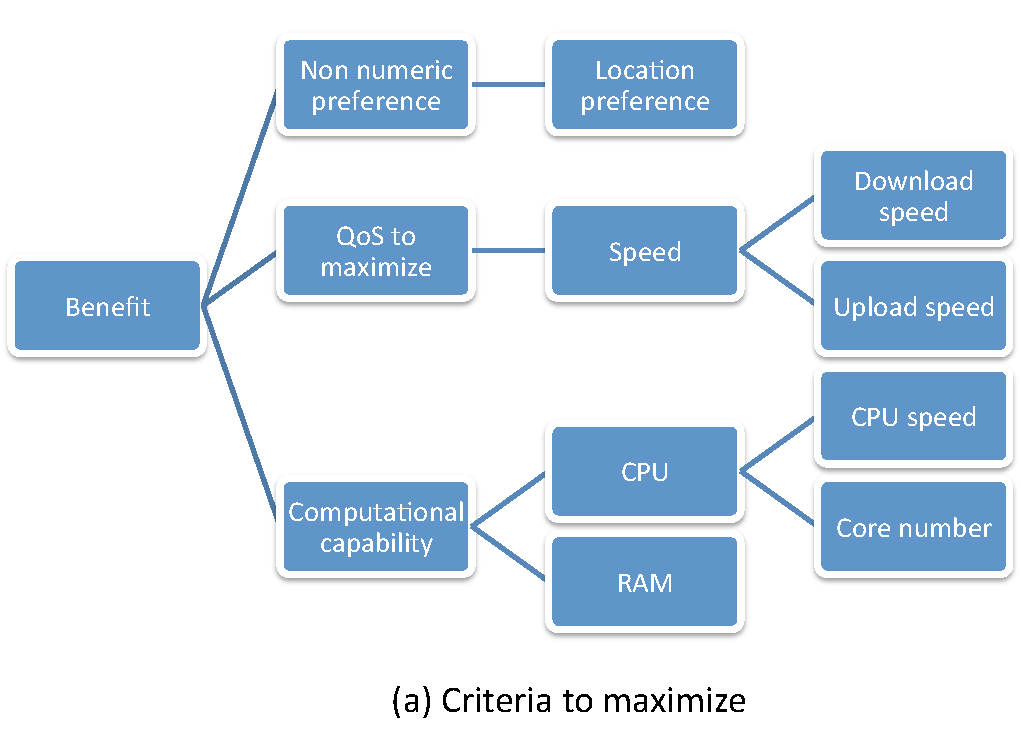
\includegraphics[width=\textwidth,keepaspectratio]{Figures/AHP/figure4a.pdf}
  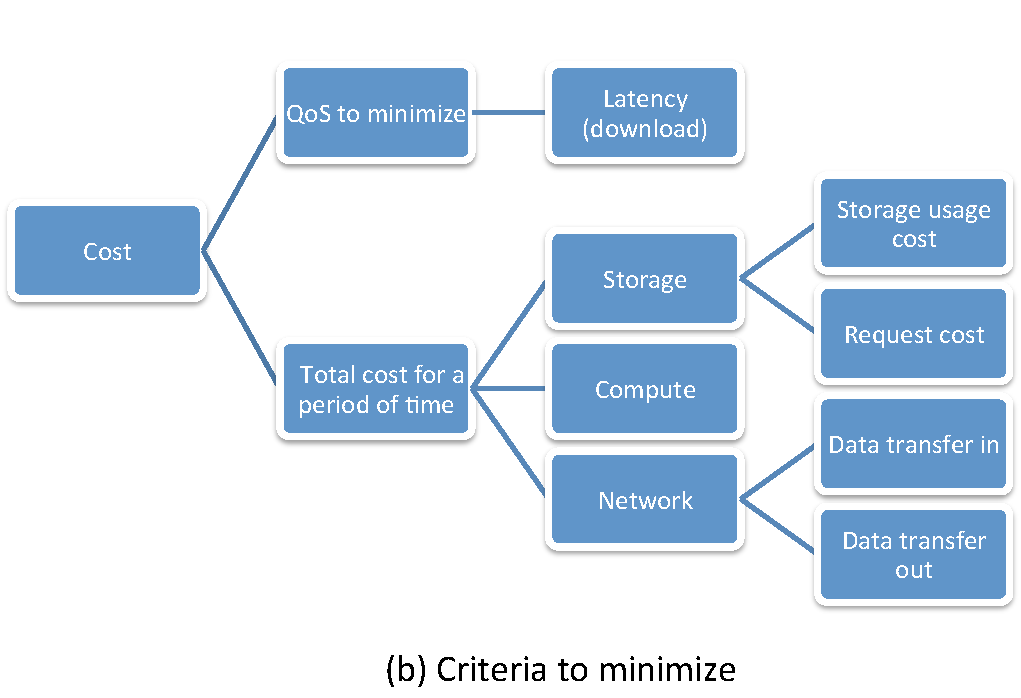
\includegraphics[width=\textwidth,keepaspectratio]{Figures/AHP/figure4b.pdf}
 \caption{ Criteria taken into consideration during comparison. There are 2 categories: benefit and cost. ``Benefit" groups the ``good" criteria which are meant to be maximized. Similarly, ``Cost" groups the ``bad" criteria to be minimized. The actual values to be collected and stored are at the ``leaf" (i.e. Node/criterion with no children) of the ``tree". For example, under ``Benefit", numeric values are collected for ``Download/Upload Speed", ``CPU Speed" and ``Number of Cores". ``QoS to Maximize" is the parent/big category ``Download/Upload Speed" belongs to, there is no value stored for this node.}
\label{fig4}
\end{figure}

$\widetilde{criteria}$ means the normalized criteria values, thus $\reallywidetilde{criteria_{beneficial}}$ means the normalized value of beneficial criteria.
For beneficial criteria, normalization is carried out by dividing each value with the highest value among options. For non beneficial criteria, we need to divide each value with the minimal value in options.

As we named this ratio \enquote{Cost Benefit Ratio}, we put cost on the numerator and benefit in the denominator. As a result we will be looking for smaller ratio as better option. Reversing numerator and denominator can still work, just means bigger ratios indicating better option.

In our decision making framework, we consider the following QoS statistics: download latency ($\zeta$), download speed (D) and upload speed ($\mu$). Those characteristics are important for end-users experience and satisfaction. It is possible to have options that have small price difference, or when having high quality service is more important than saving money.

Since users are likely to select a combination of compute storage and network services, hence the summation over resources when calculating the cost.

Note that the network QoS of Compute and Storage Service are both collected then separately stored, since user maybe only interested in one of the services. For example, transferring files from (and to) the compute instance relatively local mounted storage is different from downloading or uploading files from/to dedicated network storage service (like AWS S3 \cite{S3}). In case user select both, we use the average. For instance, in the equation we used $\bar D$ to denote that we take the average of $D_{compute}$(download speed measured from the Compute service) and $D_{storage}$  (download speed measured from the Storage service).

\subsubsection{Weight computed by Pairwise Comparison}
\label{sec:weight&pairwise_comparison}
The weight is calculated based on AHP's pair wise comparison method. We choose the commonly used scale    \cite{ghodsypour1998decision}   \cite{haas2005illustrated} shown in Table \ref{table:scale}. In case user chooses to treat all options equally, weights all become 1.

\begin{table}[!ht]
\begin{center}\caption{ABSOLUTE VALUE AND CORRESPONDING DESCRIPTIVE SCALE REPRESENTING RELATIVE IMPORTANCE} \label{table:scale}
\begin{tabular}{|c|c|c|}
\hline
\textbf{Scale }&  \textbf{Value } & Reciprocals\tnote{1}$*$ \\
\hline equal & 1 & 1\\
\hline moderate & 3 & 1/3 \\
\hline strong & 5 & 1/5 \\
\hline very strong & 7 & 1/7 \\
\hline extreme & 9 & 1/9\\
\hline
\end{tabular}
\begin{tablenotes}
  \item[1] $*$If activity i has one of the above nonzero numbers assigned to it when compared with activity j, then j has the reciprocal value when compared with i.
\end{tablenotes}
\end{center}
\end{table}

Otherwise, weight is calculated as shown in Table \ref{table:weight}. 
The meaning of symbols is explained in Table \ref{table:weight_explanation_symbols}.

\begin{table*}[!ht]
\begin{center}
\caption{Illustrating How To Turn Pair-wise Preference Into Global Weight.}
\label{table:weight}
\begin{tabular}{ccccccc}
& $V_{speed_{upload}}$ & $V_{speed_{download}}$ & $V_{ram}$ & $V_{compute_{disk}}$ & Row Sum & Weight \\
$V_{speed_{upload}}$ & 1 & ${x_{1}}$ & ${x_{2}}$ & ${x_{3}}$ & ${y_{1}}$ & ${y_1}/\tau$  \\
$V_{speed_{download}}$ & $1/{x_1}$ & 1  & ${x_{4}}$ & ${x_{5}}$ & ${y_{2}}$ & ${y_2}/\tau$  \\
$V_{ram}$ & $1/{x_2}$ & $1/{x_4}$ & 1 & ${x_{6}}$ & ${y_{3}}$ & ${y_3}/\tau$ \\
$V_{compute_{disk}}$ & $1/{x_3}$ & $1/{x_5}$ & $1/{x_{6}}$ & 1 & ${y_{4}}$ & ${y_4}/\tau$ \\
& & & & Column Sum & $\tau$ & \\
\end{tabular}
\end{center}
\end{table*}

\begin{table}[!ht]
\begin{center}\caption{Symbols Used In Weight Explanation.} \label{table:weight_explanation_symbols}
\begin{tabular}{|c|c|c|}
\hline
\textbf{Symbol }&  \textbf{Meaning } \\
%\textbf{benchmark }& \textbf{mode} &
%\textbf{ mode}  & \textbf{ mode}\\
\hline $\tau $ & The maximum value of y: $ max(y_{1},y_{2},y_{3},y_{4}) $ \\
\hline V & Value given by User to rate the importance. \\
\hline $V_{compute_{disk}}$ & How important is the size of disk space on VM. \\
\hline $V_{cost}$ & Importance value for cost. \\
\hline ${V_{latency}}$ & Importance value for Download Latency. \\
\hline $V_{ram}$ & How important is the size of memory allocated to VM. \\
\hline $V_{speed_{upload}}$ & Importance value for Upload Speed. \\
\hline $V_{speed_{download}}$ & Importance value for Download Speed. \\
\hline x & Some user input value. \\
\hline y & Sum of the row values. \\
\hline ${y_1}$ & $\left( {\sum\limits_{n = 1}^{n = 3} {{x_n}} } \right) + 1$ \\
\hline ${y_2}$ & $\left( {\sum\limits_{n = 4}^{n = 5} {{x_n}} } \right) + 1 + \frac{1}{{{x_1}}}$\\
\hline
\end{tabular}
\end{center}
\end{table}

AHP method consists of repeated matrix squaring to compute the eigenvector, as calculated in \Cref{table:weight}, every tiny improvement on precision of the eigenvector gained is at the cost of expensive computation, this is supposed to be repeated until no big enough difference can be observed. In our case, we noticed that the improvement is so small after the first squaring, we actually do not need that much of precision, so we relaxed the rule to only do one matrix squaring.

For example, user may have preference like shown in Table \ref{table:weight_example}. It will produce the preference matrix $M_1$, shown in \eqref{matrix:m1}.
\begin{equation}\label{matrix:m1}
\begin{array}{c}
    M_1\\
    \begin{bmatrix}
        1 & 1/3 & 1/5 & 1/5 \\
        3 & 1   & 3   & 5 \\
        5 & 1/3 & 1   & 3 \\
        5 & 1/5 & 1/3 & 1\\
    \end{bmatrix}
\end{array}
\end{equation}

\begin{table}
\begin{center}
\caption{Example User Preference.}
\label{table:weight_example}
\begin{tabular}{@{}c@{}c@{}c@{}c@{}c@{}}
& $V_{speed_{upload}}$ & $V_{speed_{download}}$ & $V_{ram}$ & $V_{compute_{disk}}$ \\
$V_{speed_{upload}}$ & 1 & 1/3 & 1/5 & 1/5 \\
$V_{speed_{download}}$ & & 1 & 3 & 5 \\
$V_{ram}$ & & & 1 & 3 \\
$V_{compute_{disk}}$ & & & & 1 \\
\end{tabular}
\end{center}
\end{table}

Table \ref{table:example_eigenvector} shows the steps breakdown to compute the eigenvector from \eqref{matrix:m1} before matrix squaring.

\begin{table}[ht]
\begin{center}
\caption{Example Eigenvector Calculation.}
\label{table:example_eigenvector}
\begin{tabular}{ccccccccccccc}
  &   &        &   &        &   &     &    & Row Sum &           & & Eigenvector\\
1 & + & 0.3333 & + & 0.2    & + & 0.2 & =  & 1.7333  & 1.7333/13 &=& 0.1333 \\
3 & + & 1      & + & 3      & + & 5   & =  & 13      & 13/13     &=& 1\\
5 & + & 0.3333 & + & 1      & + & 3   & =  & 9.3333  & 9.3333/13 &=& 0.7179\\
5 & + & 0.2    & + & 0.3333 & + & 1   & =  & 6.5333  & 6.5333/13 &=& 0.5026\\
\end{tabular}
\end{center}
\end{table}

If we square the matrix \eqref{matrix:m1} we get \eqref{eq:m1square}.
\begin{equation}
\label{eq:m1square}
\begin{array}{c}
    M_1 \times M_1 =
    \begin{bmatrix}
        4      & 58/75 & 22/15  & 8/3 \\
        46     & 4     & 124/15 & 98/5 \\
        26     & 44/15 & 4      & 26/3 \\
        184/15 & 98/45 & 34/15  & 4\\
    \end{bmatrix}\\
\end{array}
\end{equation}

\begin{table}[ht]
\begin{center}
\caption{Eigenvector Calculation: Matrix Squaring}
\label{table:eigenvecto_mamtrix_squaring}
\begin{tabular}{c|cccc}
\toprule
Parameter                & Without Squaring & $M^{2}$      & $M^{2^{2}}$  & $M^{2^{3}}$\\
\midrule
$V_{speed_{upload}}$     & 0.1333307692     & 0.1143835616 & 0.144178027  & 0.1407611299\\
$V_{speed_{download}}$   & 1                & 1            & 1            & 1 \\
$V_{ram}$                & 0.7179461538     & 0.5342465753 & 0.547842341  & 0.5449403125\\
$V_{compute_{disk}}$     & 0.5025615385     & 0.2659817352 & 0.3099713172 & 0.303706707\\
\hline
Change                   &                  & -0.018947208 & 0.029794465  & -0.003416897\\
                         &                  & 0            & 0            & 0 \\
                         &                  & -0.183699579 & 0.013595766  & -0.002902029\\
                         &                  & -0.236579803 & 0.043989582  & -0.006264610\\
\bottomrule
\end{tabular}
\end{center}
\end{table}

The eigenvector calculated from \eqref{eq:m1square} is \eqref{eq:eigenvector2}.
\begin{equation}
\label{eq:eigenvector2}
\left[ 
\begin{array}{c} 
0.1144 \\ 
1 \\
0.5342 \\
0.2660
\end{array} 
\right] 
\end{equation}

If we keep do this matrix squaring, the results are shown in table \Cref{table:eigenvecto_mamtrix_squaring}.
The change of value in the new eigenvector is vary small after the first squaring, so we decide to just do squaring once. If we only need the accuracy to 1 decimal place, we will use the values from the first squaring rounded to $[0.1, 1, 0.5, 0.3]$.
And if we pretend we have also calculated preference for cost and latency to be 0.8 and 0.2 as an example, the overall rank can be calculated as shown in \Cref{eq:ratio_example}.
\begin{equation}\label{eq:ratio_example}
\frac{
    0.8 \reallywidetilde {\sum { ( a_{c,l,r} P_{c,l,r} T_{c,l,r} ) } }
    + 0.2 \widetilde{ \overline{ \zeta_{c,l,r} } }
}{
    0.1 \widetilde{ \overline{\mu_{c,l,r}} }
    + \widetilde{ \overline{D_{c,l,r}} }
    + 0.5 \reallywidetilde{ \sum{M_{c,l,r}} }
    + 0.3 \reallywidetilde{ \sum{S_{c,l,r}} }
}
\end{equation}
Where $M$ represents memory size and $S$ is storage size.

\subsection{Algorithm}
It is more likely that users choose to use a single provider to eliminate costly cross-provider data transfer, but others may have the need to use multiple providers to achieve greater coverage and disaster resilience.

We have abstract our approach in Algorithm \ref{algo:orderedSolutions}. Most of the symbols can be found in Table \ref{table:algo_symbols} and \ref{table:relational_algebra_set}, some symbols are defined earlier in \Cref{table:formula_symbols} and \ref{table:weight_explanation_symbols}. We have separated the relational algebra and set operations into Table \ref{table:relational_algebra_set}, please pay attention to operation G as it has multiple inputs represented by superscript and subscripts.

\begin{table}[!ht]
\begin{center}\caption{Symbols Used In Algorithm.} \label{table:algo_symbols}
\begin{tabular}{|c|p{10cm}|}
\hline
\textbf{Symbol }&  \textbf{Meaning} \\
\hline AvgQoS &   Table/Relation contains the QoS data collected \\
\hline ${D_{compute}}$ &   Download speed from the compute instance \\
\hline ${D_{storage}}$ &   Download speed from pure storage, i.e. S3 \\
\hline $\bar D$ &   Average download speed calculated as: $\frac{1}{2}\left( {{D_{{\rm{compute}}}} + {D_{storage}}} \right)$ \\
\hline $\ell$ &  
$\ell  \subseteq L$  Some set of locations which are specified by the user, by default 
 $\ell  = L$, which means consider all locations available.
 \\
\hline $M_{min}$ & Minimum memory requirements of compute instance/server  \\
\hline $pric{e_{\max }}$ &   The maximum price one is willing to spend \\
\hline $\rho$ &   
$\rho  \subseteq C$ Some set of  Cloud  providers which are specified by  the user; by
default   $\rho  \subseteq C$, which means consider all locations available. \\
\hline ${\Re _{compute}}$ &  Table/Relation contains all data collected about Compute resources.  \\
\hline ${\Re _{network}}$ &  Table/Relation contains all data collected about Network resource. \\
\hline ${\Re _{storage}}$ & Table/Relation contains all data collected about Storage resource. \\
\hline $\bar \mu $ &   Average upload speed, similar to $\bar D$ \\
\hline U & A tuple representing the estimated usages provided by user, containing the
following: $( U_{compute} , U_{storage} , U_{data_{in}} , U_{data_{out}} )$\\
\hline W & A tuple representing the preference/weight given to each component by the user, it consists of the following: 
$( W_{compute} , W_{storage}, W_{network} $ , $ W_{download} , W_{upload}, W_{latency} )$ \\
\hline
\end{tabular}
\end{center}
\end{table}

\begin{table}[!ht]
\begin{center}\caption{Symbols Used In Algorithm: Relational Algebra and Set Operations.} \label{table:relational_algebra_set}
\begin{tabular}{|c|p{10cm}|}
\hline
\textbf{Symbol }& \textbf{Meaning } \\
\hline 
G & 
    Aggregation operation over a schema, like a \textbf{group by} clause in SQL.
    It follows the format:
    $\tensor[_{a_g}]{G}{_{agg\_op(attri)}} (r)$
    where $a_g$ is the grouping attribute.
    $agg\_op(attri)$ is the aggregation operation over attribute (attri). 
    There are five aggregate functions that are included with most relational database systems.
    These operations are Sum, Count, Average, Maximum and Minimum.
    \textbf{r} is an arbitrary relation.
    See relationa algebra wiki page \cite{ref36} for more details.\\
    
\hline $\sigma $ &  Selection, see wiki page \cite{ref36}.\\
\hline $\bowtie$ & Natural join: depends on the condition can be either $\theta$-join or equijoin. For example, $\bowtie(Provider,Location)$ means equijoin where the condition is join only under the same provider and location\\
\hline  $ \cup$  & Set union operation. \\
\hline $\mapsto $ & Ordered pair, here we use it to denote a new record being formed. The reason we used it is because $storageCostByQuota$ maps storage options to a set of costs, i.e. for the same kind of storage option it maps to multiple storage tires, with different unit prices; thus $storageCostByQuota: \Phi _{storage} \to \mathcal{P}(\mathbb{R})$ where $\mathcal{P}(\mathbb{R})$ means the power set of real numbers, for example for a value x, we can have $storageCostByQuota(x)=\{1,2\}$, and the total cost for x is 1+2=3.\\
\hline
\end{tabular}
\end{center}
\end{table}

\begin{algorithm}[float,caption={orderedSolutions $( \ell , {M_{\min }} , price_{\max} , \rho , U , W )$}, label={algo:orderedSolutions}]
//Filtering on the static characteristics
${\Phi _{compute}}: = {\sigma _{provider \in \rho  \wedge location \in \ell  \wedge memory \ge {M_{\min }}}}\left( {{\Re _{compute}}} \right)$

//Link it with QoS statistics.
${\varphi _{compute}}: = {\Phi _{compute}}{{\rm \bowtie}_{provider,location,serviceName}}AvgQoS$
${\Phi _{storage}}: = {\sigma _{provider \in \rho  \wedge location \in \ell  \wedge quot{a_{low}} < {\upsilon _{storage}}}}\left( {{\Re _{storage}}} \right)$

//Calculating storage price for each tier.
storageCostByQuota:= empty
foreach ${x_s} \in {\Phi _{storage}}$ do
    if ${U_{storage}} > quota_{max}({x_s})$ then
        $storageCostByQuota \cup
        \left\{ x_s \mapsto ( quota_{max}(x_s) - quota_{min}(x_s) )\cdot unitPrice({x_s}) \right\}$
    else
        //Usage is less or equal to the storage tire max quota
        if ${U_{storage}} > quota_{min}({x_s})$ then
            $storageCostByQuota \cup
            \left\{ x_s \mapsto ( U_{storage} - quota_{min}(x_s) ) \cdot unitPrice(x_s) \right\}$
        end
    end 
end

//Combining storage cost in different tiers to get total.
$storageCost: = \tensor[_{service\_name\;\&\;provider}]{G}{_{sum(storage\_cost)}} (storageCostByQuota)$
${\varphi _{storage}}: = storageCost{\bowtie_{provider, location, serviceName}}AvgQoS$
${\Phi _{network}}: = {\sigma _{provider \in \rho\;\wedge\;location \in \ell\;\wedge\;quot{a_{low}} < {\upsilon _{storage}}}}({\Re _{network}})$

//Match appropriate Compute, Storage and Network options.
$\varphi : = {\varphi _{compute}}{\bowtie_{provider,\;location,\;location_{client}}}{\varphi _{storage}}{\bowtie_{provider,\;location}}{\Phi _{network}}$

totalCost: = empty
foreach $x \in \varphi$ do
    $totalCost(x) = \sum {( U_r P_r )}$
end

// Find unit values for normalization
minCost:= min(totalCost(x)); $\forall x ; x \in \varphi$
$minAvgLatency:=min(\bar \zeta)$
$maxAvgUplinkSpeed:=max(\bar \mu)$
$maxAvgDownlinkSpeed:=max(\bar D)$
$maxToTalMemory:=max(\sum M)$
$maxToTalStorage:=max(\sum S)$

rank: = empty
foreach $x \in \varphi$ do
    $rank(x) =
    \frac{
        W_{cost} \frac{totalCost(x)}{minCost}
        + W_{latency} \frac{\bar \zeta_r}{minAvgLatency} 
    }{
        W_{upload} \frac{\bar \mu_r}{maxAvgUplinkSpeed}
        + W_{download} \frac{\bar \mu_r}{maxAvgDownlinkSpeed}
        + W_{memory} \frac{\sum M_r}{maxToTalMemory}
        + W_{storage} \frac{\sum S_r}{maxToTalStorag}
    }
    $
end

return sortOnRankDescending(rank)
\end{algorithm}

Algorithm \ref{algo:orderedSolutions} only depicts one common use case, other scenario exists but can be solved with a simplified version of the algorithm or with small modification/addition. We will explains these situation in the following paragraphs.

As shown in Algorithm \ref{algo:orderedSolutions}, a user can provide us the following inputs $( \ell , M_{\min } , price_{\max} , \rho , U , W )$. $\ell$ is the set of locations that a user wants to consider, by default we consider all locations. $M_{\min}$ is the minimal memory requirements for the VMs, 0 denotes no memory requirements. $price_{\max}$ is the maximium budget user willing to spend, 0 indicating they are only interested in free services, -1 is used to represent infinity which means there is no budget constrains. $\rho$ is the set of Cloud service providers that a user wants to consider, by default we consider all providers. $U$ represents the the estimated usages of all the resources: $( U_{compute} , U_{storage} , U_{data_{in}} , U_{data_{out}} )$. $U_{compute}$ is the number of instances, $U_{storage}$ is the number of GB of storage will be used. $U_{data_{out}}$ is the amount of outward data transfer in GB from Cloud provider to end devices/users. Similarly, $U_{data_{in}}$ represents the amount of inward data transfer. All the previously mentioned usage estimations are all monthly based, but other length can be used such as daily or hourly, as long as all resource are calculated based on the same standard, there should be no effect on the final comparison and ordering. $W$ represents a user's preference, details are explained in Section \ref{sec:cost_benefit_ratio} and \ref{sec:weight&pairwise_comparison}.

Once options satisfy user requirements have been identified, we calculating price according to different model. There are various pricing models    \cite{weinman2011axiomatic} exist, for example, free, flat-rate, two-part tariffs (like the AWS reserved instance), block-declining (S3 storage), bidding (AWS spot instance). They can mostly be incorporated into our model except the bidding type. One provider often have multiple offers within the same type of services, for example, different kind of instances for the compute service, different storage options, we combine them to get a combinatorial number of choices, we do that for all providers, then calculate the summed cost and rank for each combined option. Not all users need all 3 types of resources, if they specify 0 for a type of resource, it will not be considered. But network service is always needed.

\subsection{QoS Profiler}
\label{sec:QoSProfilerDesign}
We implement a QoS Profiler service that helps in collecting network QoS values from different points on the Internet (modeling big data source location) to the Cloud data centers.
We collected the statistics using the \enquote{speedtest} service provided by CloudHarmony.

Klein et al. \cite{klein2012towards} proposed a highly theoretical model based on Euclidean distance for estimating latency, which we believe their theoretical perfect distance assumption can not be practically accurate. However, we can use this model to estimate latency when QoS data is not available for a new client location.

The QoS profiling system consists of multiple agents at geographically dispersed locations to collect and process data, shown in Fig \ref{fig:QoSMonitoringServiceNetworkTopology}.
If we look at individual slave node, we can see every node profiles the QoS statistics to various Clouds from each location. Bashed scripts are written to export data from each node. Master node pulls data from its children nodes, access keys are required for this operation. Then the CSV formatted data is imported to the master database, where appropriated merge operation is performed. For more implementation details please refer to Chapter \ref{cha:system}.

\begin{figure}[!ht]
 \centering
 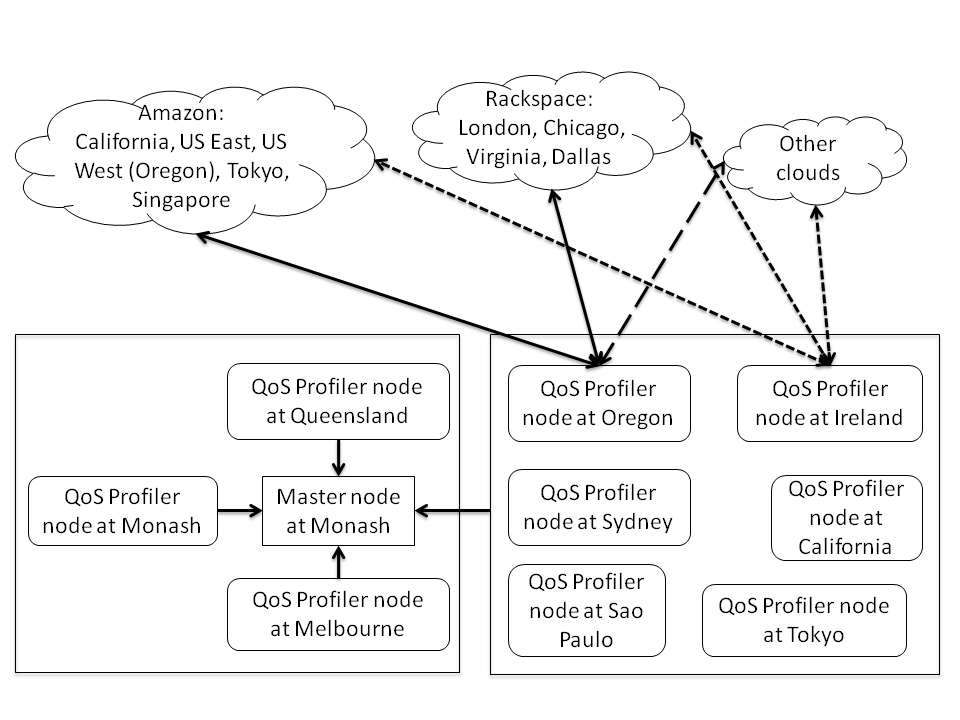
\includegraphics[width=\textwidth,keepaspectratio]{Figures/QoS/figure2.png}
 \caption{QoS Monitoring Service Network Topology. We have used 2 Clouds namely: Nectar Research Cloud and Amazon Web Service. Since Nectar Cloud is free for researchers, we kept the instances running all the time, hence the decision to put master node in Nectar. Because there is a limit of quota in Nectar and Amazon have greater geographical coverage in terms of data-center locations. We use additional Spot instance from Amazon as slave data crawlers. A QoS Monitoring Node profiles Download Speed, Latency and Upload Speed at each datacenter in various Clouds from different locations.}
\label{fig:QoSMonitoringServiceNetworkTopology}
\end{figure}

Initially, the QoS data was collected on slave node every 2 hours by running the ``speedtest'' service of CloudHarmony. A single run takes more than an hour to finish hence we are collecting it once every two hours. Later by analyzing the data, we conclude that such high frequency is not necessary, because the average QoS from a particular location to a particular data center most of the time fluctuating in a small range. That means the average would be pretty stable. We can use historical data as a pretty reliable indication. Note that difference between data-centers and various locations are still huge as expected, see Fig. \ref{fig:DownloadSpeedFromAmazonToMelbourne}. In the future we may allow a combination of real time and off-line values to be used if necessary.

\begin{figure}[!ht]
 \centering
 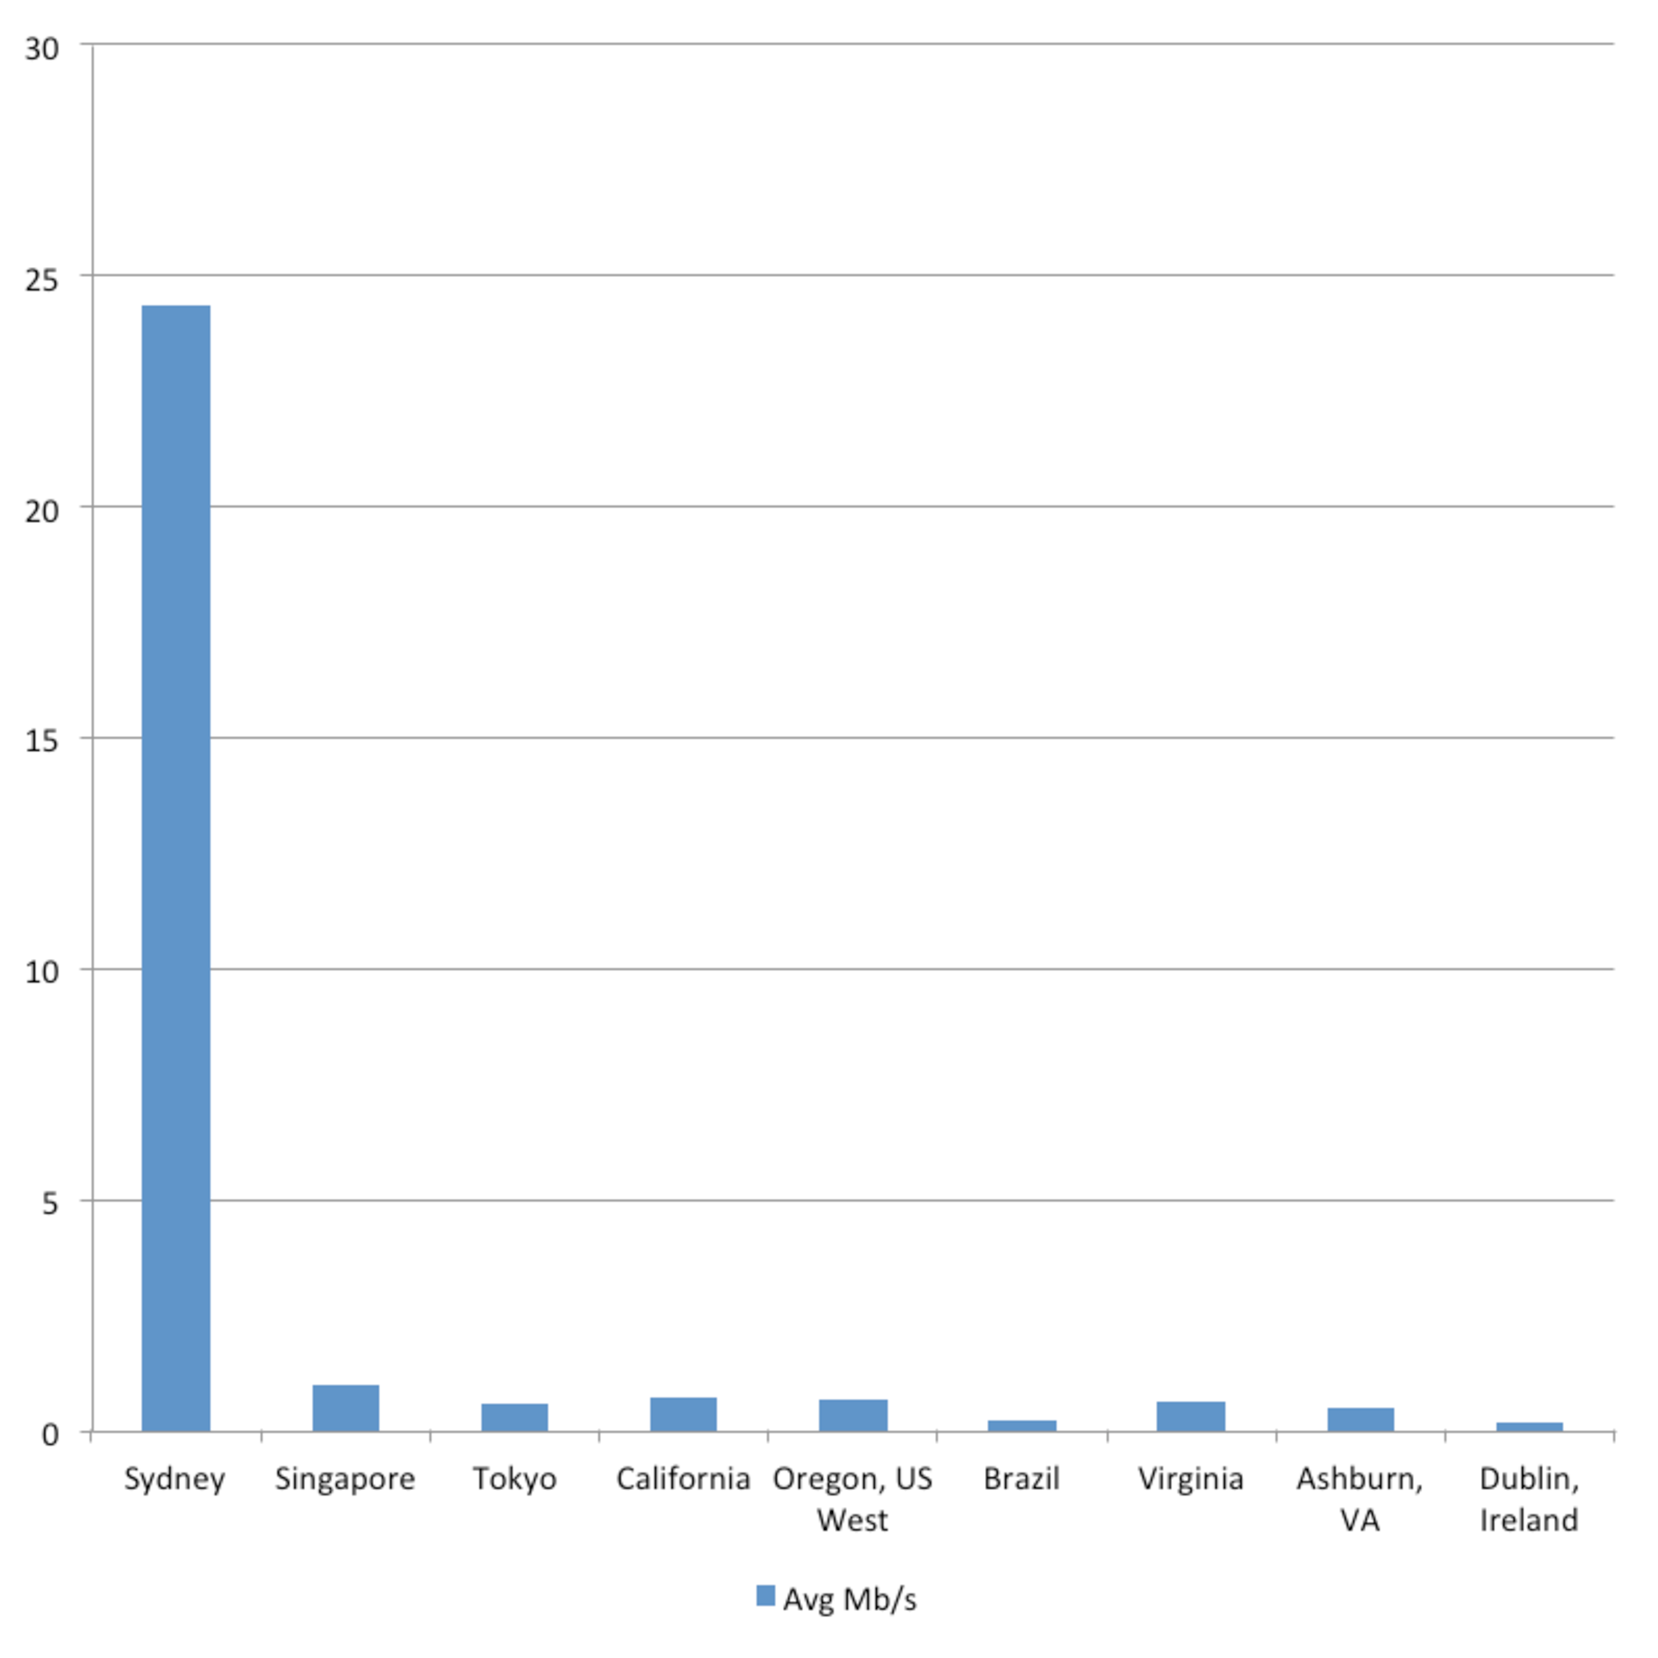
\includegraphics[width=\textwidth,keepaspectratio]{Figures/QoS/figure5.pdf}
 \caption{Download speed from Amazon data centers to Melbourne}
\label{fig:DownloadSpeedFromAmazonToMelbourne}
\end{figure}

\Cref{fig:DownloadSpeedFromAmazonToMelbourne} shows that geographically close data center has (as high as 25 times) better network performance, hence this validates the fact that location is one of the important criteria which should be considered during selection process. Our measurements also indicate that distance is not the only factor that affects the network performance, as shown in Fig. \ref{fig:DownloadSpeedAgainstDistance}, data centers are ordered from closest to furthest, and from left to right, Tokyo and Brazil clearly perform poorly than expected. Hence, we consider the need for active probing and profiling of network QoS from user's endpoint connection to the Cloud data centers. By doing so, we get a clear picture of data centre's network QoS from the users' device that may be deployed across topologically distributed network locations. Note that we have left out Sydney on purpose. Fig \ref{fig:DownloadSpeedFromAmazonToMelbourne} shows the exponential increase in speed between Sydney and Melbourne compare to overseas locations, while Fig \ref{fig:DownloadSpeedAgainstDistance} shows the linear relationship between downloading speed and distance among overseas locations. We are aware that while it is generally true that the geographical distance between any pair of servers (or users) on the Internet affects the route trip time (RTT), the bandwidth between them is not necessarily determined by the distance, many other aspects can affect the user end QoS, like the last-mile home-connecting technology, local Internet traffic condition. Our measurements are only providing suggestive base for further optimisation, user's actual experience will vary.

\begin{figure}[!ht]
 \centering
 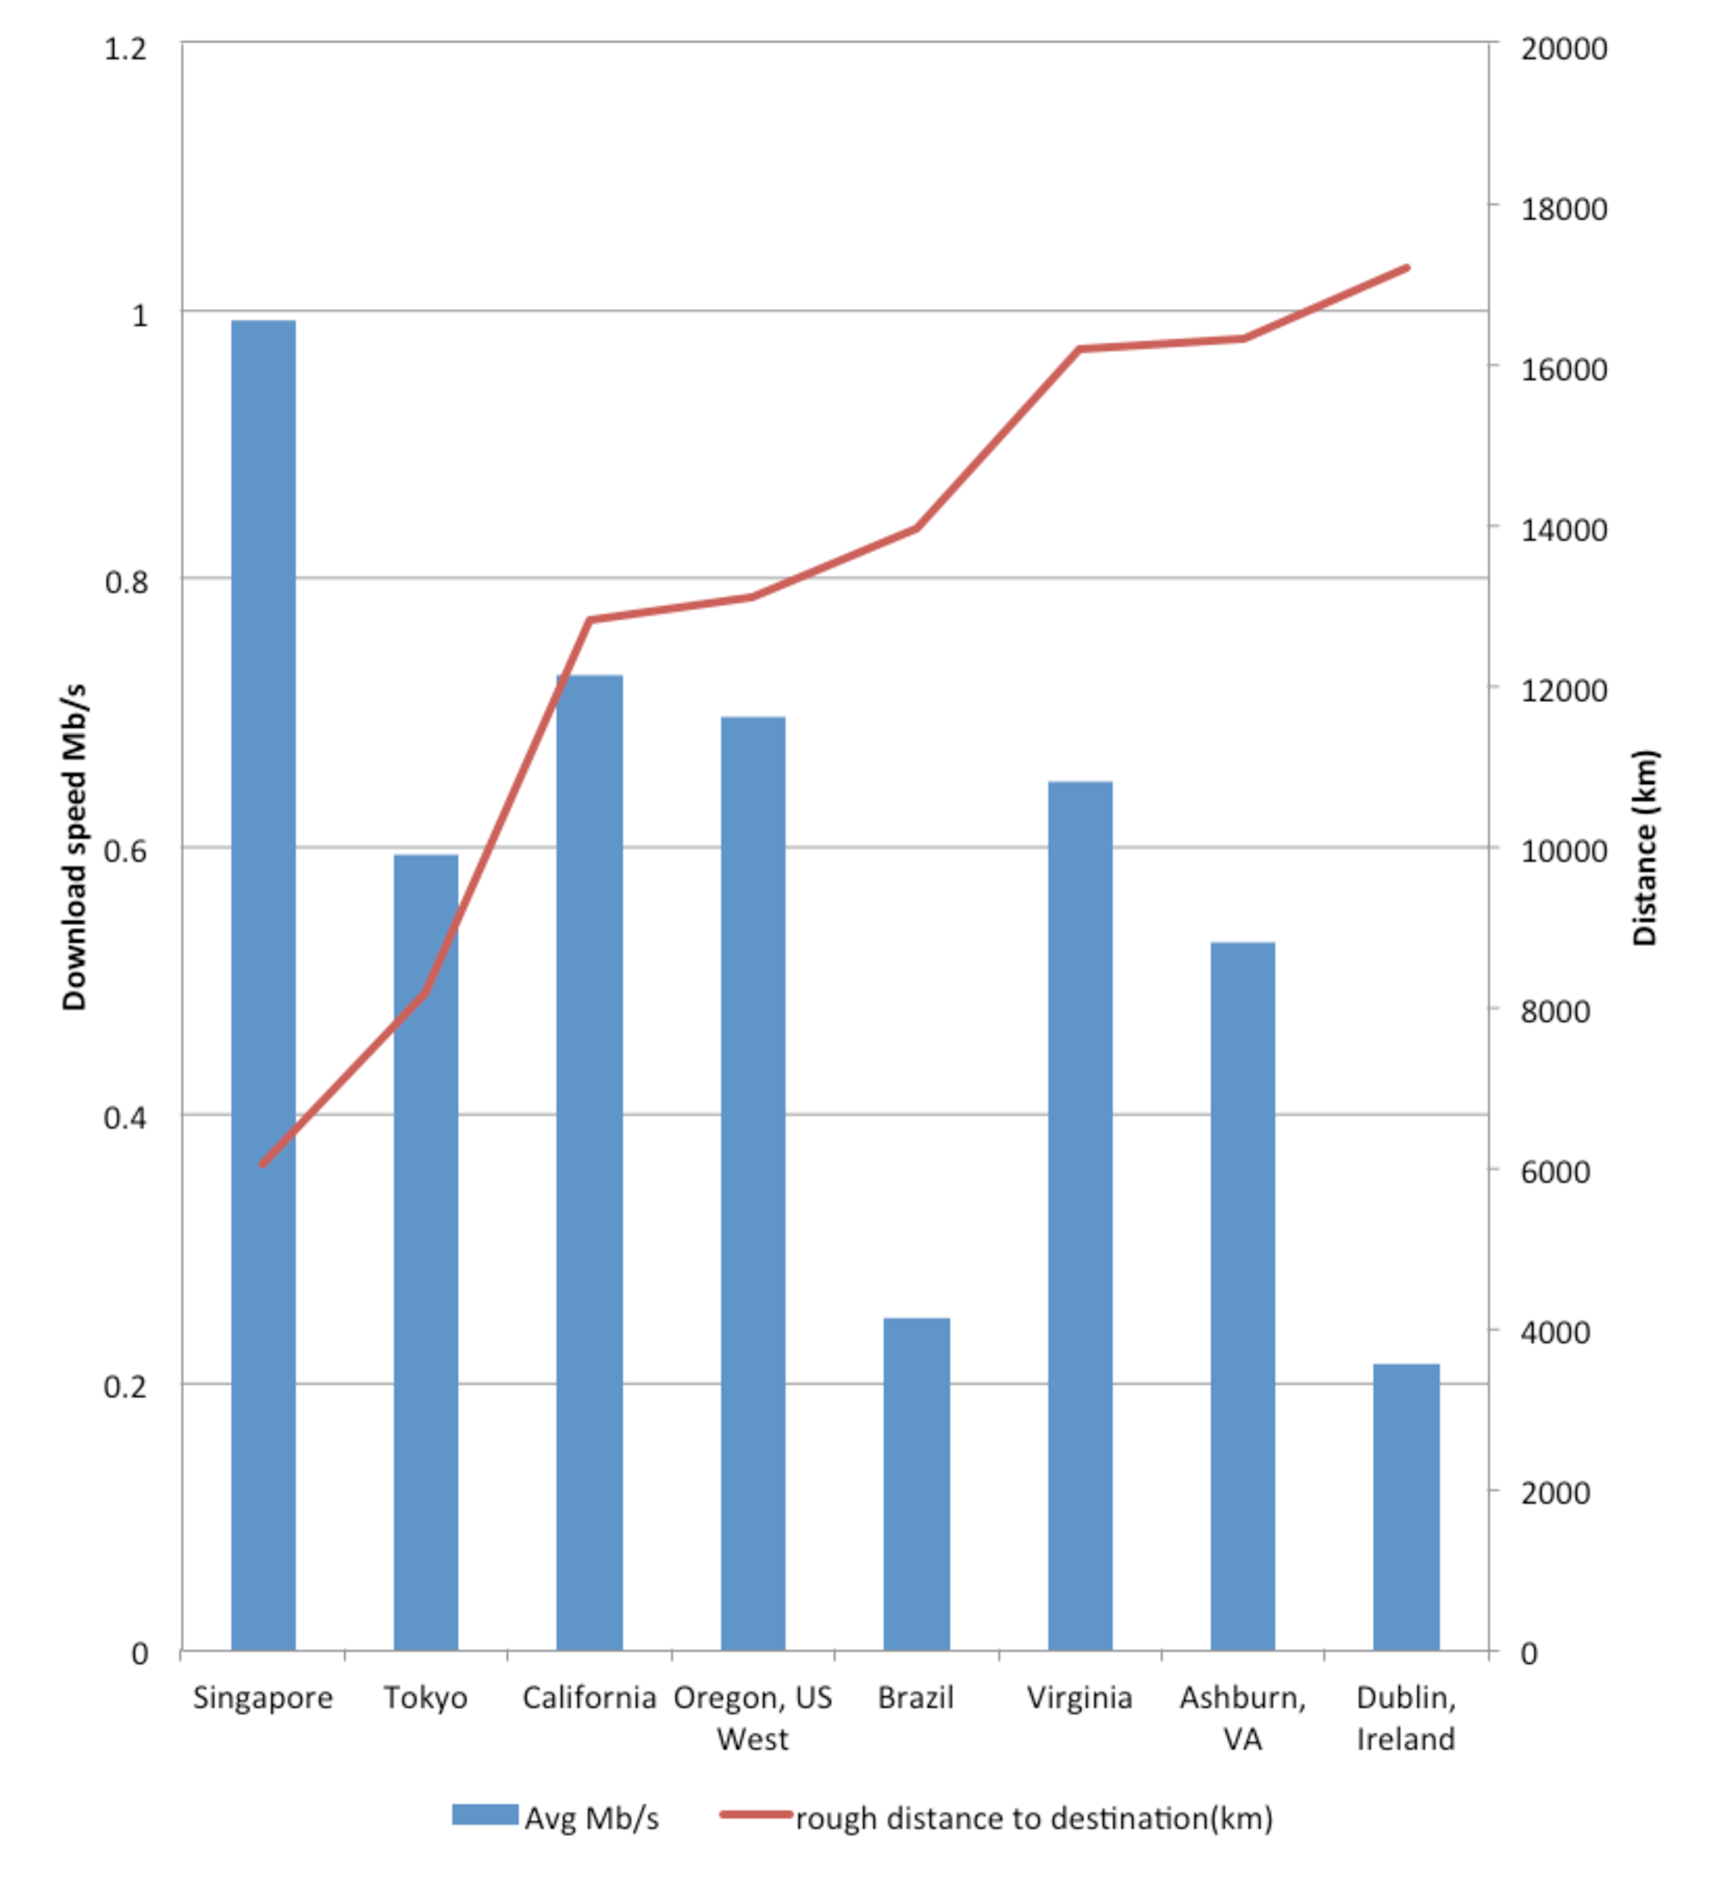
\includegraphics[width=\textwidth,keepaspectratio]{Figures/QoS/figure6.pdf}
 \caption{Download Speed Against Distance.}
\label{fig:DownloadSpeedAgainstDistance}
\end{figure}

\section{Experiments}
\subsection{Setup}
We run our system and proposed algorithmic technique across a range of hardware systems to understand the implication of hardware resource configuration (see Table \ref{table:experiment_env}) on the performance of the approach.

\begin{table}[!ht]
\begin{center}\caption{Experiment Environments} \label{table:experiment_env}
\begin{tabular}{|p{5mm}|p{30mm}|p{25mm}|p{15mm}|p{25mm}|>{\hspace{0pt}}p{15mm}|}
\hline
\rotatebox[origin=c]{90}{\textbf{Environment}} &  \textbf{Description } &  \textbf{Processor Speed }&  \textbf{Memory}&  \textbf{Processor Name }&  \textbf{Role }\\
%\textbf{benchmark }& \textbf{mode} &
%\textbf{ mode}  & \textbf{ mode}\\
\hline
1 & MacBook Air Physical machine &    1.4 GHz &  2 GB &  $\;$ Intel Core 2 Duo & Master  \\
\hline
2 & Ubuntu 12.04.3 LTS instance ina virtualized environment & 2.4 GHz (1vCPU) & 4 GB & AMD Opteron (TM) Processor 6234 & Master / Profiler\\
\hline
3 & Standard Small (m1.small)Linux / UNIX EC2 Spot Instance & 1.79 GHz ( 1ECU / vCPU) & 1.7 GB & Intel(R) Xeon(R)CPU E5-2650 & Profiler\\
\hline
4 & Compute Optimized(c3.8xlarge) Linux/UNIX EC2Spot Instance & 2.8 GHz (32 vCPU 1081 ECU) & 60 GB & Intel(R) Xeon(R)CPU E5-2680v2 & Performance Testing \\
\hline
\end{tabular}
\end{center}
\end{table}

To summarize, Environment 1 is the local machine used during the development of the program, which is capable of running the database and other system modules.

Environment 2 is the server from The National eResearch Collaboration Tools and Resources (NeCTAR) Cloud \cite{NeCTAR} where the our system can be deployed as a service which is easily accessible over the Internet. It is a virtualized environment, so the CPU speed labeled may not accurately reflect the actual allocation.
NeCTAR's infrastructures are located at at eight different organisations (node sites) around Australia. It operates as one Cloud system under the Openstack framework. This makes it having different UI and API compare to AWS. Being a collaborative research Cloud, it is only open to affiliated members (i.e. Australian researchers, students from participating university). Although the access is free, there is a limitation of 2 instance per member and a cap on the total resource usage. 

Environment 3 is the spot instance type (from Amazon) we used to collect QoS statistics from additional locations, but to cut down the cost; we kept the usage minimal.

Environment 4 is the compute optimized spot instance type we used to test program performance under a powerful CPU, or vertical scalability in short.

\subsection{Case Study}
\subsubsection{Input Parameters}
Table \ref{table:input_param} shows the primary configurable parameters of our algorithm. Everyone's requirements regarding the compulsory parameters usually vary. So we choose a range of values to mimic different selection scenarios. In future work, we may conduct user survey to understand the most concerned factors for different type of users, for example we can exposed all possible constrainable parameters via the API but it may not be necessary (not to mention also slows down the processing) and it will only overwhelm the users who only uses the visual interface. Optional parameters are the one tend to be hard to specify (especially for users with less technical background). Default value column shows what we use when not specified.

\begin{table}[!ht]
\begin{center}\caption{Input Parameters.} \label{table:input_param}
\begin{tabular}{|l|r|}
\hline
\textbf{Compulsory }&  \textbf{Example Value } \\
%\textbf{benchmark }& \textbf{mode} &
%\textbf{ mode}  & \textbf{ mode}\\
\hline Storage(GB/30 Days) & 20 \\
\hline Outbound Data Transfer(GB/30 Days) & 50 \\
\hline Min RAM(GB) & 4 \\
\hline \textbf{Optional } & \textbf{Default Value} \\
\hline Provider Brand & Consider All \\
\hline Display Currency  & AUD \\

\hline Number of Hours to run (per Month) & 720 \\
\hline Number of Instance needed (per Month) & 1 \\
\hline Inbound Data Transfer(GB/30 Days) & 1  \\
\hline Weight of Compute Cost(percentile) & $35\%$ \\
\hline Weight of Storage Cost(percentile) & $25\%$ \\
\hline Weight of Network Cost(percentile) &  $35\%$\\
\hline Weight of Latency(percentile) & $5\%$ \\
\hline Weight of Download Speed(percentile) & $70\%$ \\
\hline Weight of Upload Speed(percentile) & $30\%$ \\
\hline Max RAM(GB) & $100\%$ \\

\hline
\end{tabular}
\end{center}
\end{table}

\subsubsection{Results}
Figure \ref{fig7} shows the top $5\%$ of the result we get from the inputs in Table \ref{table:input_param}. It is in ascending order of ratio (cost over benefit) as indicated by the dotted (blue) line, because lower cost over higher benefit gives us a smaller ratio which representing a better choice.  If we look at ranking by considering only the cost, as illustrated by the solid (red) line, the GoGrid offers dominate over Windows offerings. If to order results in ascending price order (means network QoS constraints are not considered), shown in Fig. \ref{fig8}, Azure disappears from the top $10\%$ of choices. Similarly, we can see that although the price change is small in solutions, their overall rankings are greatly different (dotted blue line). What this means to users is that while we can save money by ignoring network QoS but then they should be ready for degraded network performance Note that although we tried out best in using real world data, sometimes Cloud providers vary their prices as frequent as weekly. However, in future work we intend to implement a price crawler service that will automatically parse the provider's web pages and update our system's database.

\begin{figure}[ht]
    \centering
    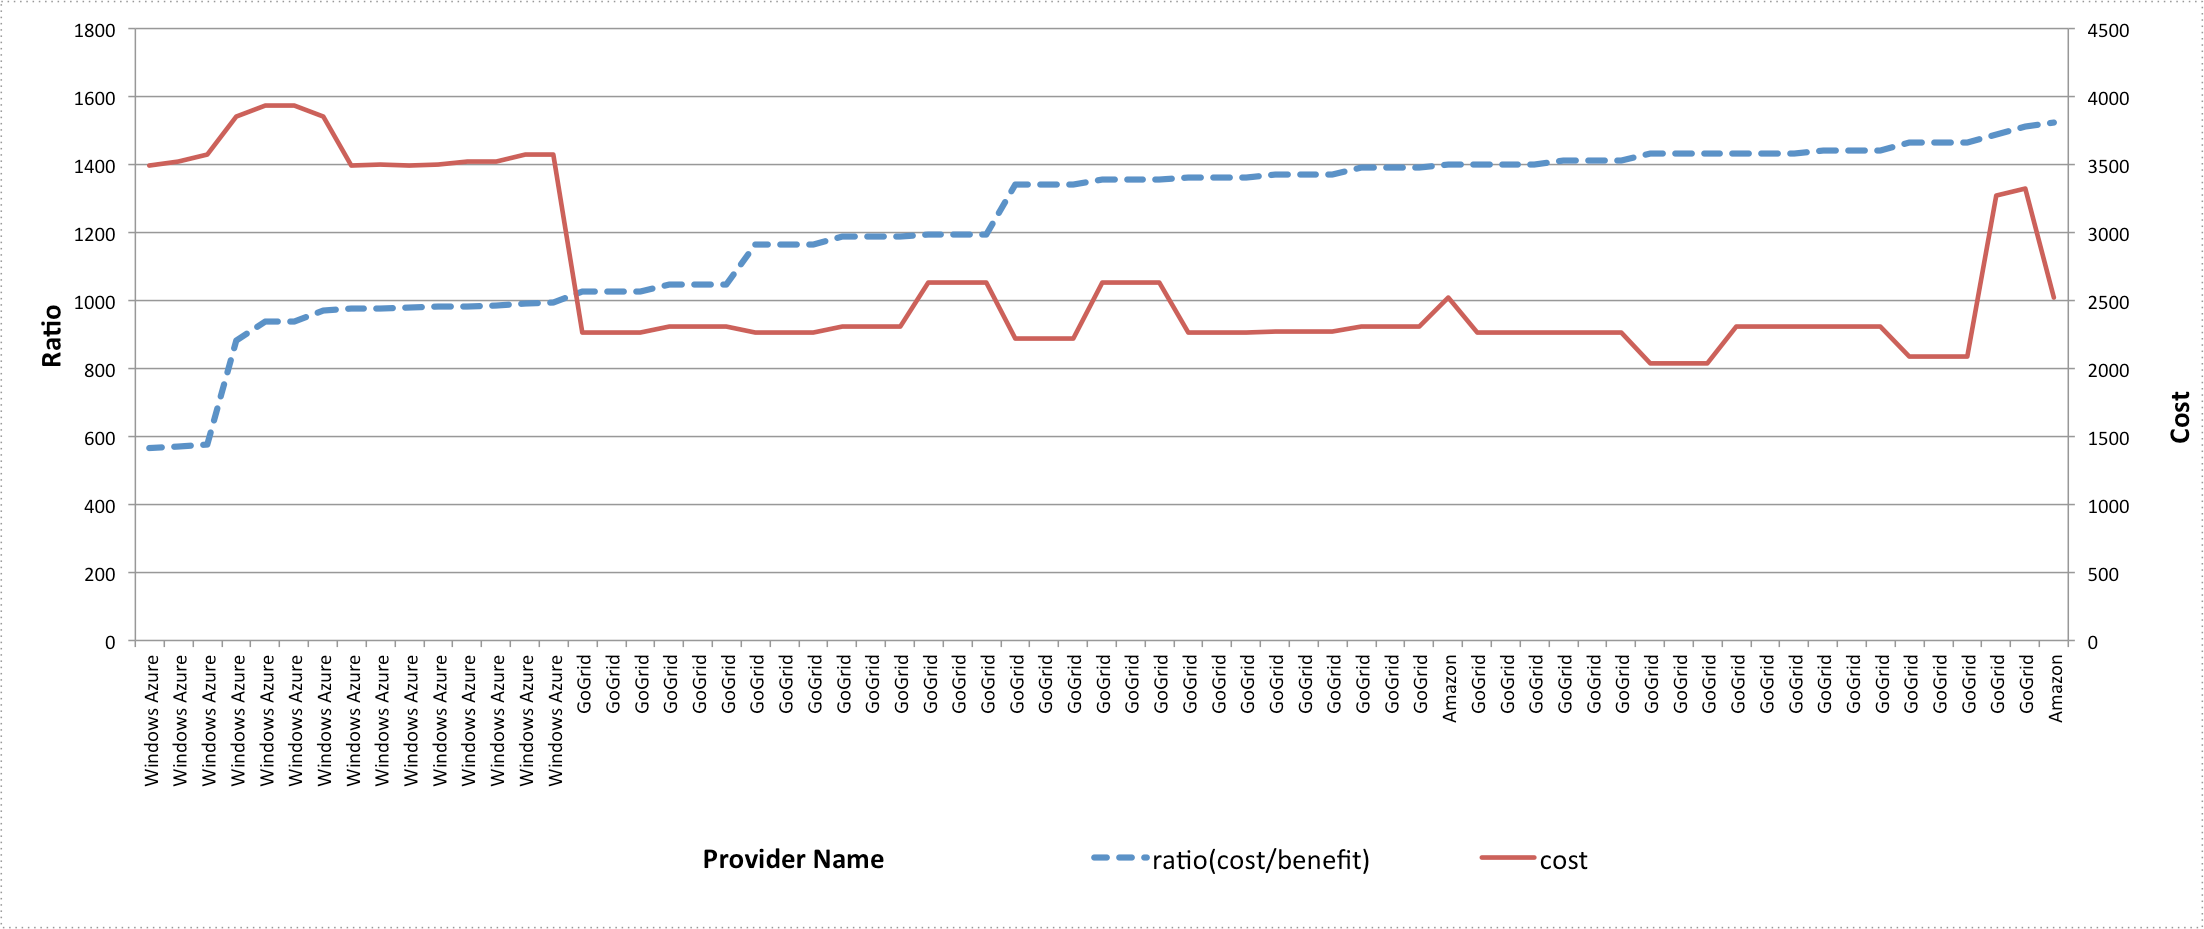
\includegraphics[angle=-90, scale=0.6]{Figures/AHP/figure7.pdf}
    \caption{Results in ascending order by (cost / benefit) ratio}
    \label{fig7}
\end{figure}

\begin{figure}[ht]
 \centering
 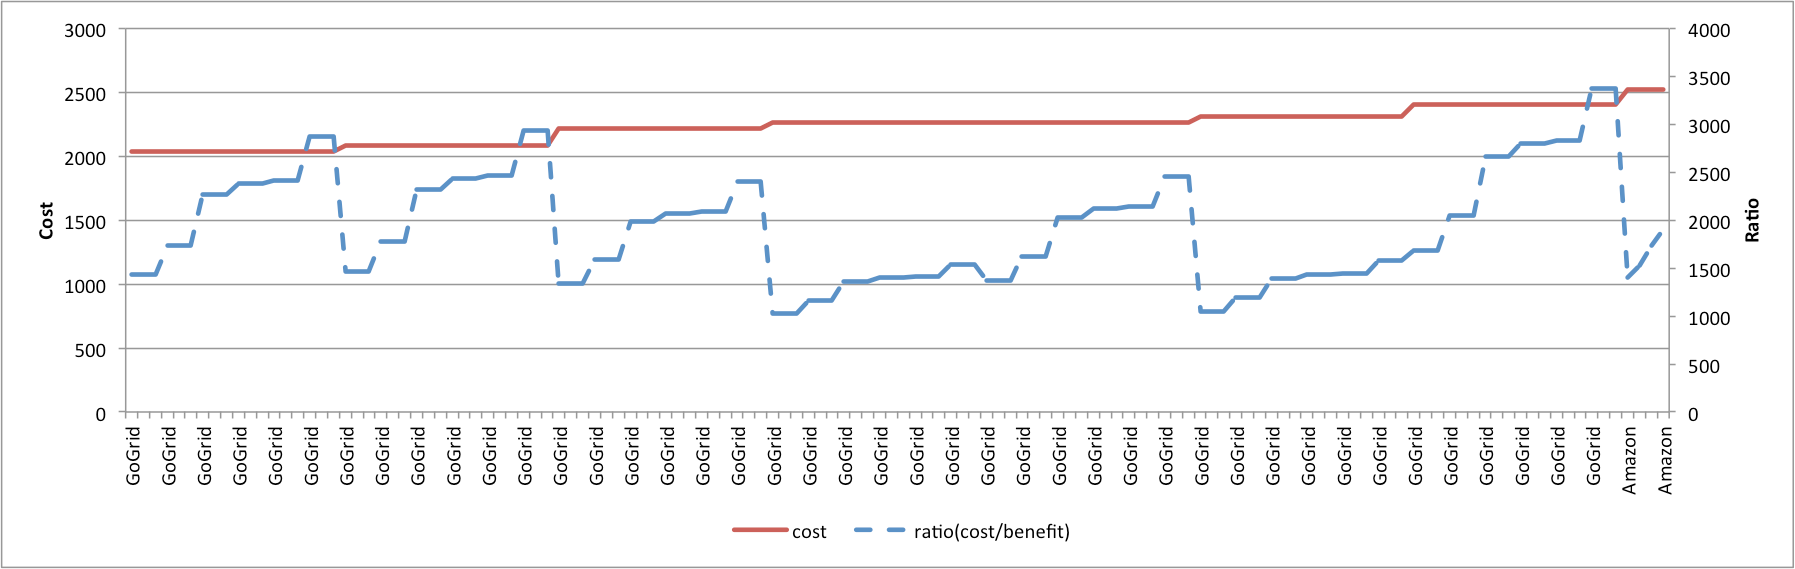
\includegraphics[angle=-90, scale=0.7]{Figures/AHP/figure8.pdf}
 \caption{Results in ascending order by cost}
\label{fig8}
\end{figure}

\subsubsection{Performance}
The average run time for our current solution is about 11 seconds, with cache turned on in MySQL, we get up to $9\%$ improvement on the same query. As the constraints become stricter the solution space reduces, as a result processing time decreases (to as low as 4.97 seconds), see Table \ref{table:avg_runtime}.

\begin{table}[htbp]
\begin{center}\caption{Average Runtime.} \label{table:avg_runtime}
\begin{tabularx}{\textwidth}{|X|X|p{2cm}|X|X|X|X|X|}
\hline
Test Number &Storage (GB/30 Days) &Outbound Data Transfer (GB/30 Days) & Min RAM (GB) &  Row(s) & \rotatebox[origin=c]{90}{Enviroment 1} &\rotatebox[origin=c]{90}{Enviroment 2} &\rotatebox[origin=c]{90}{Enviroment 4}\\
\hline 1 & 20 & 10 & 0 & 3808 & 12.04 & 11.07 & 10.96   \\
\hline 2 & 40 & 15 & 0 & 3808 & 11.913 & 11.59 & 7.81\\
\hline 3 & 10 & 2 & 0 & 3808 & 11.169 & 10.76 & 7.05 \\
\hline 4 & 20 & 2 & 0  & 3808 & 11.744 & 11.15 & 7.57 \\
\hline 5 & 200 & 200 & 0  & 3808 & 11.894 & 11.72 & 7.49 \\
\hline 6 & 200 & 200 & 0  & 3808 & 11.912 & 10.85 & 6.76 \\
\hline 7 & 200 & 200 & 16  & 552 & 9.15 & 7.7 & 4.97 \\
\hline 8 & 200 & 200 & 8  & 1524 & 9.644& 9.69 & 5.53 \\
\hline 9 & 200 & 200 & 4  & 2095 & 10.25 & 8.72 & 5.58 \\
\hline 10 & 20 & 20 & 0  & 3808 & 12.06 & 11.51 & 7.03 \\
\hline \multicolumn{5}{|r|}{Average} & 11.1776 & 10.476 & 7.075\\
\hline
\end{tabularx}
\end{center}
\end{table}

The performance increase observed when we move from environments 1 to 2 then 4 is resulted from an increase of processing power, hence the idea of "scale up". There is a limit to the amount of processing power one core can have, but our solution is single threaded at the moment, there is still room for improvement by utilizing all cores (like environment 4).  In the future we will explore the option of configuring MySQL/InnoDB to use multithreads (Default is 4 and maximum is 64 since MySQL 5.1.38). Then we will decide whether we need to "scale out".

\subsection{Computational Complexity}
We define the upper bound computational complexity of our optimization approach as shown in \eqref{eq:computational_complexity}.
\begin{equation} \label{eq:computational_complexity}
O\left( {\left| R \right| \times \left| C \right| \times \left| L \right| + \left( \frac{(|\nu|-1)|\nu|}{2}\right)} \right)
\end{equation}

In cost estimation, we have to calculate prices for $|R|$ resources, $|C|$ providers, and $|L|$ geographical locations. In case a more complex utilization function is given, the computational complexity may increase.

In our current model, we consider $|v|$= 6, see weight calculation in Table \ref{table:weight}. Hence to determine the weights in the benefit-cost ratio evaluation function, 15 pair-wise comparisons have to be made, unless user choose to use the default values. In both cases this part of the complexity factor is a constant which can be omitted.
\chapter{Resource Usage Estimation}
\label{cha:ResourceUsageEstimation}
Decisions to migrate existing systems to public IaaS clouds can be complicated as evaluating the benefits, risks and costs of using cloud computing is far from straightforward. Furthermore, given the large number of cloud instance types even for a single datacenter (such as AWS), it is not easy to select the type of server instance let alone determine the entire cloud infrastructure as choosing different instance types has different impacts on cost and performance and such decision making information is not readily available in a succinct and organized manner.

Aiming to eliminate potential bottlenecks for users to take advantage of cloud computing, this paper presents an improved system (which extended the previous work) that further allows informed users (i.e. infrastructure architects, CIOs, system admins) to make multi criteria selection and comparison on IaaS offers considering various bench-marking results. 

The proposed technique is applicable to selecting Infrastructure as a Service (IaaS) cloud offers, and it allows users to define multiple design-time and run-time requirements. These requirements are then matched against our knowledge base to compute possible best fit combinations of cloud services at IaaS layer. 

Quality of Service (QoS) is an important concept in the context of cloud service. When deploying services in a cloud environment, it is necessary to consider and evaluate the impact of network QoS on the performance of underlying user applications/services. Among all the performance characteristics, QoS characteristics, including latencies, network bandwidth, etc, are as important as other ones, such as CPU, memory and disk resources. From cloud service providers’ perspective, they care about QoS very much and heavily invest in it because it has direct impact on user experience. 

In our previous work on QoS aware cloud service selection we have compared the network performance; in this paper we will investigate some higher level metrics e.g. benchmark for web server, database, analytics application. Application level metrics can give a more precise measurement of how good the overall system completes assigned tasks.

In our experiments we  applied simple and Queuing Theory \cite{queueing_theory} model to estimate best fit resource allocation for achieving target Service Level Agreements (SLA).

\section{Related Work}

There is a number of studies \cite{lee:10,RodrigoICPP,xuzichuan} applied Queuing Theory in their Cloud provisioning mechanism. Since we do not focus on real time provisioning or load balancing, we only use a Queuing Theory based method to estimate the required number of VMs. 

PlanForCloud \cite{PlanForCloud}, provides a web-based tool for calculating costs on the IaaS cloud. PlanForCloud enables sophisticated modeling of the components of cloud deployments, including servers, storage, databases and data transfers, as well as usage scenarios that incorporate growth, seasonality and other variability in the consumption of cloud resources. Users first design prospective deployments by creating cloud services such as servers, storage and databases. Then, this runs the prospective deployments through a simulation engine to create a detailed three year cost report. It can be used to clone deployment, change options and growth patterns to do what-if analysis. This tool, like previously discussed cost calculators assumes that users know their cloud configuration set-up
and want to compare different cloud providers.

The AWS sizing tool developed by CopperEgg \cite{AWS_Sizing_Tool} aims to solve the problem of selecting the most appropriate EC2 instance for a given application. CopperEgg claims that the AWS sizing tool accurately benchmarks enterprise and cloud servers to help customers choose the proper Amazon EC2 instance types, pricing, and Elastic Block Storage (EBS) configurations from over 200 possible Amazon Web Services (AWS) combinations. This tool benchmarks the actual user application and matches the most appropriate EC2 instance. However it is limited to only AWS EC2 instances and also requires the application to be run over a 24 hour period before providing a decision.

\section{Problem Abstraction}
\subsection{Description}
There are Application developers/companies considering renting Cloud Infrastructure, for example it would be beneficial for them to estimate how many servers the need to achieve certain performance, and associated total costs of such setting.
There are different kind of servers/VMs that are available from different Cloud providers(with various costs).
There is also different locations of data centers one can choose from each provider. Each kind of server may have a slight different RAM capacity and CPU speed, which would result in different speed for processing the same job.

\subsection{Aim}
I would like to estimate the system performance, give benchmarking results (servicing time) for certain tasks. And predict/simulate system behavior under different constrains, e.g. total cost, maximum wait time. 

For example , a company maybe owning 4 servers with configuration (4GB, 1.8GHz CPU), but they need to expand their business in a new country and support double the number of customers they currently support. They want to evaluate the option to move the in house infrastructure to Cloud, they could run benchmark software on their servers, to get the service time for their business operations, like they can run Jmeter to get the number of web requests they can handle per second (i.e. 20) for the overall cluster (4 machines). 
Then They can run the same benchmark software on one of the Cloud servers(maybe with 16GB RAM 3.6GHz CPU), they may get a 10 request per second result.
The simplest way to estimate number of cloud servers needed would be, they just get 2 of this Cloud servers to achieve 20 requests per second (average/peak time) performance.

This is the part I'm trying to work out at the moment.

If we consider modeling the application (to be migrated to the new environment i.e. a public Cloud Infrastructure) as queuing system.

In an commercial web application scenario, customers would send requests to the server, when load is heavy it would be queued (in a buffer). Let's call the customers requests "jobs".
The job arrival may not follow any pattern, this is the part I'm not quite sure about.

Last time I showed you how I did the calculation, assuming the job arrival is Poisson, i.e. the probability of next job arrival only depends on the last one, but not anything before the last, which is also called memoryless.

\subsection{Kendall’s Notation}
In Queuing theory, Kendall’s Notation denotes a system by

A/B/m/K/n/D,

where

A: distribution function of the inter-arrival times

B: distribution function of the service times

m: number of servers

K: capacity of the system, the maximum number of customers in the system including the one being serviced

n: population size, number of sources of customers

D: service discipline.

Exponentially distributed random variables are notated by M, meaning Markovian or memoryless.
Furthermore, if the population size and the capacity is infinite, the service discipline is FIFO, then they are omitted.

For example M/M/r/K/n stands for a system where the customers arrive from a finite-source with n elements where they stay for an exponentially distributed time, the service times are exponentially distributed, the service is carried out according to the requests’ arrival by r severs, and the system capacity is K.

\begin{center}
\begin{longtable}{p{27mm} p{106mm}} 
\caption{Notations: Symbols Used in the Formulas} \label{table:symbols} \\
\hline
Symbol & Represents \\ 
\hline
\characteristicslpv\ & Function returns the characteristic features of VM type $Ty_{l,p,v}$, like CPU speed, number of cores, etc.\\
$Ch_{req}$ & Features required by a Customer, $Ch_{req} \ \subset \ \characteristicsset$. \\
L & Set Of Locations that a customer want to consider (e.g. $L = \{AU,SG,NL\}$ which stands for Australia, Singapore and Netherlands). \\
P & Set of Providers (e.g. $P = \{Amazon, GOGrid\}$). \\
Ty & VM type set is the set of tuple $\{L \times P \times V\}$. \\
$V$ & Set of VM types (e.g. $V = \{Small, Medium, Large\}$). \\
\costlpv\ & Renting Unit price of VM type $Ty_{l,p,v}$. \\
\hline
\multicolumn{2}{l}{Queuing Model Symbols}\\
\hline
$n$	        & Number of instances or servers.\\
$duration$ & Duration of test in seconds.\\
$ job{\_}count$ & Number of job send during the test. There are different types of jobs; in web, it could be GET or POST Http requests; in analytical application, it would be a specific task, like word count (map reduce); in a SQL or NoSQL database, it would be a query (i.e. SELECT * FROM some{\_}table).\\
$\lambda$ & Arrival Rate (Rate of arrival of jobs), calculated by: $\lambda=\frac{duration}{job{\_}count} $ 
In web application, it would be the number of requests received per second.\\
$T_{s}$ & Service Time (Average time taken to service a job). In Jmeter it is call "Latency". Measured in milliseconds, converted to seconds.\\
$\mu$ & Service Rate. Job processed per unit time. For example, to get the number of jobs processed per second $\mu=\frac{\textbf{1 second}}{T_{s}}$ \\
$\rho$ & Server utilization or traffic intensity or agent occupancy. The utilization of the system is the ratio between the rate of arrivals and the rate of service. $\rho =\frac {\lambda }{n \mu}$, where n is the number of servers.
In Queuing Theory, it is used to describe how busy the system is, or how far away is the system is to its theoretical limit.  In situations when the system is considered busy or under heavy traffic, different formulas needed to be used for approximation.This value will be between 0 and 1. If it is not less than 1 then the agents are overloaded, and the Erlang C calculations are not meaningful, and may give negative waiting times.\\
$\sigma$    & Standard deviation. Specifically for service time distribution in this paper.  \\
var[S] & Variance of the service time. The variance of a data set is calculated by taking the arithmetic mean of the squared differences between each value and the mean value, which is also standard deviation squared, i.e. $\sigma^{2}$.\\
$CV$ & CV is the coefficient of variation of the service time distribution. $CV=\frac{\sigma}{mean}=\frac{\sigma}{T_{s}}$\\
$T_{r}$ & Total response/delay/waiting time. In a queuing system, a customer's time is spent either waiting for service or getting service. $T_{r}=T_{w}+T_{s}$\\
\hline
\multicolumn{2}{l}{$T_{w}$ calculation in different Queuing Models}\\
\hline
$E[W^{M/M/1}]$ & Average waiting time for M/M/1 queue. $E[W^{M/M/1}]= \frac{\rho}{ \mu(1-\rho) }$\\
$E[W^{M/G/1}]$ & Average waiting time in M/G/1 queue. $E[W^{M/G/1}]=\frac  {\rho ^{2}+\lambda ^{2} var[S]}{2\lambda (1-\rho )}$\\
\hline
$E[W_{H}^{M/G/1}]$ & Heavy traffic approximation for wait time. $E[W_{H}^{M/G/1}]=\frac{ \lambda (  \frac{1}{\lambda ^{2}} + var[S]) }{ 2(1-\rho ) }$ \\
$ero_{H}$ & The relative error of the heavy traffic approximation. $ero_{H}=\frac{ 1-\rho ^{2} }{ \rho ^{2}+\lambda ^{2} var[S] }$\\
\hline
$E[W^{M/M/n}]$	& Average delay/waiting time in M/M/n or M/M/c queue. $E[W^{M/M/n}] =\frac{ C(n,\frac{\lambda}{\mu}) }{n\mu-\lambda} + \frac{1}{\mu}$\\
$C(n,\frac{\lambda}{\mu})$ & Erlang's C formula. $C(n,\frac{\lambda}{\mu})$ is the probability that an arriving customer is forced to join the queue (all servers are occupied).$ C(n,\frac{\lambda}{\mu}) = \frac {1}{ 1+(1-\rho)\frac {n!}{ (n\rho )^{n} } \sum _{k=0}^{n-1}{\frac { (n\rho )^{n} }{ n! }} } $ where $\rho$ is the server utilization, $n$ is the number of servers.\\
\hline
$E[W^{M/G/n}]$	& Average delay/waiting time in M/G/n or M/G/k queue. $E[W^{M/G/n}]= \frac{CV^{2} +1}{2}E[W^{M/M/n}]$\\
\hline
\multicolumn{2}{l}{Pricing Model Symbols}\\
\hline
$price_{VM}$ & Unit price of Virtual Machine.\\
$price_{storage}$ & Renting Unit price of storage per GB. \\
$price_{network}$ & Unit price for outward data transfer per GB.\\
$n_{storage}$ & Estimated storage need in GB.\\
$Co_{storage}$ & Storage cost. $Co_{storage} = n_{storage} price_{storage}$\\
$Co_{network}$ & Network cost. $Co_{network} = n_{network} price_{network}$ \\
$Co_{total}$ & Total cost. $Co_{total} = price_{VM} n + Co_{storage} + Co_{network}$ \\
\hline
\multicolumn{2}{l}{constraint satisfaction symbols}\\
\hline
$B_max$ & Budget of Customer.\\
$R_{max}$ & Maximum response time limit set by the customer.\\
$Th_{min}$ & Minimum throughput requirement.\\
\hline
\multicolumn{2}{l}{Ranking Calculation according to Preference, Analytic hierarchy process(AHP) symbols}\\
\hline
$speed_{download}$ & Estimated download speed from a vendor in GB per second.\\
$weight_{cost}$ & Computed weight factor for cost from user preference following the AHP method.\\
$weight_{ram}$ & Weight factor for RAM requirements.\\
$weight_{CPU}$ & Weight factor for CPU requirements.\\
$weight_{storage}$ & Weight factor for storage requirements.\\
$weight_{download{\_}speed}$ & Weight factor for download requirements.\\
ram & Total amount of RAM for all virtual machines (in each recommendation/suggestion).\\
ratio & \makecell{$ratio = \frac{cost}{benifit}$ = \\ 
$\frac{ Co_{total} weight_{cost} } { weight_{ram} ram + weight_{storage} n_{storage} + weight_{download{\_}speed} speed_{dowbload} }$  }\\
\hline
\end{longtable}
\end{center}


\begin{center}
\begin{longtable}{c p{100mm}}
\caption{Examples} \\
\hline
Type & Measurements \\
\hline
Light & $\lambda=1, T_{s}=0.199, \mu=5.02513, \rho=0.199$\\
Heavy & duration = 65 seconds, $job{\_}count = 85 \lambda=0.140496$ requests per second, $T_{s}$=7.117 seconds, $\mu$=0.140509 requests per second, var[S]=3.10817, $\rho$=0.999907\\
\hline
Poisson Arrival\\
\hline
Light & duration = 120 seconds, $job{\_}count = 194, \lambda=1.61667$ requests per second, $T_{s}$=0.217 seconds, $\mu$=4.60829 requests per second, $\sigma = 0.124$ seconds $\rho=0.350817$, n=1\\
Heavy & duration = 61 seconds, $job{\_}count = 87 \lambda=0.144759$ requests per second, $T_{s}$=6.509 seconds, $\mu$=0.153633 requests per second, var[S]=0.031684, $\rho=0.942235, \sigma=0.178$, n=1\\
\hline
\end{longtable}
\end{center}

\begin{center}
\begin{longtable}{c p{100mm}}
\caption{Evaluations} \\
\hline
Type & Estimation \\
\hline
Light & $T_{r} = 0.248439$\\
Heavy & $E[W^{M/M/1}] = 0.248439$\\
Heavy & $E[W^{M/G/1}] = 40817.9, E[W_{H}^{M/G/1}]=40825, ero_{H}=0.000174367$\\
\hline
Poisson Arrival\\
\hline
Light & $E[W^{M/M/1}] = 0.117266, T_{r} = 0.334266$\\
Heavy & $E[W^{M/M/1}] = 106.171, T_{r} = 112.68$\\
Heavy & $E[W^{M/G/1}] = 53.1252, E[W_{H}^{M/G/1}]=59.8337, ero_{H}=0.126278$\\
Light & $C(n,\frac{\lambda}{\mu})$ = 0.350817, $E[W^{M/M/n}] = 0.334266, E[W^{M/G/n}]=0.221707$\\
Heavy & $C(n,\frac{\lambda}{\mu})$ = 0.942235, $E[W^{M/M/n}] = 112.68, E[W^{M/G/n}]=56.3821$\\
\hline
\end{longtable}
\end{center}


\subsection{Case 1}
In the simplest 1 server 1 job type setting:

I have set up a simple web application (written in Python), it returns some result/page to the customer.

The first simple test, I used Jmeter to generate the customer workload/jobs, it sends 120 identical GET requests to the local server, between consecutive requests, there is a random wait between x and y milliseconds.

The average service time per request calculated is 199 ms. 
with average of under 10\% CPU utilization and 40\% memory usage (16*0.4= 6.4GB).
Without tuning the default web server settings, the application is not exhausting the the full potential of the hardware. 


the actual plan can be find in this Git repository

Written in Python

Local machine specification:
RAM 16 GB 
CPU 3.2 GHz



On the Google Cloud Platform results are:

I'm currently conducting more experiments, for more complex scenarios, then I may be able to compare results 
could be 
1 server multiple job types
multiple server(same type) 1 job type
multiple server(same type) multiple job types

For example in the simplest case:
Give a server type A, with RAM r

\section{System Design}
\label{sec:sys_design}



\subsection{Preference and Requirements}


\subsubsection{Location}

A customer has location constraints specified by the set $L$. We eliminate all the VM types that are not from the specified locations:
\begin{equation} \label{eq:location_constraint}
\forall\ i \in L
\end{equation}

\subsubsection{VM Characteristics}

A Customer has constraints on certain characteristics of VMs to be used, it can be mathematically written as:
          
\begin{equation} \label{eq:characteristics_constraint}
\characteristicslpv\ \in Ch_{req}
\end{equation}



\subsection{Benchmarks}
\subsubsection{Web Application}
We used Jmeter to generate the web workload.
We used a timer called "Poisson Random Timer" to give a random pause to request before they are send to server. We used a "Lambda" value of 100 ms and "Constant delay offset" value of 300 ms. For the short response GET test.
Test results has been synchronized with an on-line Blazemeter account.


\begin{table}[!htbp]
\caption{Example benchmarks provided by CloudHarmony}
\label{table:Example_benchmarks}
\begin{center}
    \begin{tabularx}{\textwidth}{|l|X|}
    \hline
    Name & Description \\ \hline
    Apache & This test profile measures how many requests per second a given system can sustain when carrying out 700,000 requests with 100 requests being carried out concurrently. \\ \hline
    DB & This metric measures performance using database server related benchmarks including mysql-bench, pgbench, redis, sqlite and tpcc-mysql. \\ \hline
    C-ray & This is a test of C-Ray, a simple raytracer designed to test the floating-point CPU performance. This test is multi-threaded (16 threads per core), will shoot 8 rays per pixel for anti-aliasing, and will generate a 1600 x 1200 image. \\ \hline    
    \end{tabularx}
\end{center}
\end{table}

Some example benchmarks provided by CloudHarmony are shown in Table \ref{table:Example_benchmarks}, i.e. Apache \cite{Apache_benchmark}, DB and C-ray.



\subsection{Simple Generalized Workload Distribution}

Let the rate a Cloud server ($i$) can process jobs be $\mu_{i}$.
Assume the user have collected some historical workload information at their own server, then the workload at time $t$ can be get from some function $f(t)$, the number of Cloud servers of type $i$ needed is calculated as:

\begin{equation}\label{eq:n}
n_i (t) = \frac{ f(t) }{\mu_{i}} 
\end{equation}

Or if the workload information is not available but same benchmark has been run against the user's private server, let $\mu_{j}$ be the benchmark result for server type $j$, user's total workload is assumed to be $n_j \mu_{j}$, then the number of servers of type i, can be estimated as follows:

\begin{equation}\label{eq:nprime}
n_i \approx \frac{ n_j \mu_{j} }{\mu_{i}} 
\end{equation}



\subsection{Queueing Theory based Model}



\subsubsection{Response Time}
The response time is the total amount of time a job spends in both the queue and in service. 



\paragraph{M/M/c queue}
If the workload follows exponential distribution, e.g. for web servers, we can model it using M/M/c queue \cite{MMc_queue_wiki}.

Let average request arrival rate be $\lambda$, for example if there are 360 jobs per minute, $\lambda$ = 360/60 = 6 jobs/second. Average Job processing rate be represented by $\mu$, the number of servers be n. If there are less than n jobs, some of the servers will be idle. If there are more than n jobs, the jobs queue in a buffer.

Server utilization is expressed as:

\begin{equation} \label{eq:rho}
a=\frac{\lambda}{n \mu}
\end{equation}

For the queue to be stable $a < 1$ is required. $a$ represents the average proportion of time which each of the servers is occupied, assuming jobs choose their servers randomly. 

The probability that an arriving job is forced to join the queue (all servers are occupied) is denoted as:

\begin{equation} \label{eq:probability_of_waiting}
C(n,\frac{\lambda}{\mu})
\end{equation}
which is referred to as Erlang's C formula \cite{erlangc}. We assume this value to be 1 to simplify the calculation. Based on queuing theory \cite{queueing_theory}, the average waiting time can be calculated as (means of notations can be found in Table \ref{table:symbols}):

\begin{equation} \label{eq:mmcq}
E[W^{M/M/c}] = \frac{ C(n,\frac{\lambda}{\mu}) }{n \mu - \lambda}+\frac{1}{\mu} 
\end{equation}  



\paragraph{M/G/k queue}
More general cases of workload distribution can be modeled by M/G/k queue \cite{MGk_queue_wiki}, and its average waiting time can be calculated as:  

\begin{equation} \label{eq:mgkq}
E[W^{M/G/k}] = \frac{1+CV_e^2}{2} E[W^{M/M/c}]
\end{equation} where $CV_e^2$ is the squared coefficient of variation of the service time distribution, which can be computed as:
\begin{equation} \label{eq:cv}
CV=\frac{\sigma}{m}
\end{equation}
where $\sigma$ is the standard deviation and m is the mean.



\subsubsection{Number of servers needed}
We feed the allocation strategy to the response time calculating function in equation \eqref{eq:mgkq}, along with the characteristics of all types of VMs we are handling, to estimate the response time, and for making it a constraint, we say it should be less than the customer requirement of response time ($R_{max}$), so by letting Equation \ref{eq:mmcq} equals to $R_{max}$, we can calculate the number of minimum machines required:

\begin{equation} \label{eq:num_machines_mmcq}
n = \frac{1}{\mu R_{max} - 1} + \frac{\lambda}{\mu}
\end{equation}

Similarly for cases when we apply M/G/k queue, we use Equation \ref{eq:mgkq}.

\begin{equation} \label{eq:num_machines_mgkq}
n = [ \, ( \, \frac{2R_{max}}{1+CV^2} - \frac{1}{\mu} ) \,^{-1} + \lambda ] \, \frac{1}{\mu}
\end{equation}



\subsubsection{Throughput Constraint}

Let the throughput achieved when response time constraint is satisfied be $\lambda\prime$, from Equation \ref{eq:num_machines_mmcq} we can induce its calculation:

\begin{equation} \label{eq:throughput_mmcq}
\lambda\prime = n\mu - \frac{\mu}{\mu R_{max} - 1}
\end{equation} 

Or from Equation \ref{eq:num_machines_mgkq} we get:

\begin{equation} \label{eq:throughput_mgkq}
\lambda\prime = n \mu - ( \, \frac{ 2 R_{max} }{1+CV^2} - \frac{1}{\mu} ) \,^{-1}
\end{equation} 
            
It should be greater than the customer requirement of $Th_{min}$.



\subsubsection{Solve by Linear Optimization}


\paragraph{Cost}
This section mainly focus on estimating computational resource. Network and storage resource usage are assume to be know (calculated from user supplied data). More details on cost calculation can be found in our previous work \cite{IJNGC2013}, and this section only represent it very abstractly. 

We multiply the number of instance with its corresponding price and how long it is estimated to be required to get the total cost.

Options are first filtered according to users preference. Let $L\prime$, $P\prime$, $V\prime$ be the set of all $l \in L$, $p \in P$, $v \in V$ satisfy $\characteristicslpv \in Ch_{req}$.

\begin{equation} \label{eq:cost}
TotalCo(L\prime,P\prime,V\prime) = \sum_{l \in L\prime, p \in P\prime, v \in V\prime} ( X_{(l,p,v)} \costlpv T_) + Co_{storage} + Co_{network}
\end{equation}

When given QoS constrains and the objective is to minimize the cost, applying Equation \ref{eq:mmcq} and \ref{eq:throughput_mmcq}:

\begin{tabbing}
mmm  \=mmmmmmmmmmmmmmmmmmmmmmmmmmmmmmm \kill
min \> $TotalCo(L\prime,P\prime,V\prime)$ \\
{\it s.t.}  \> $\frac{ 1 }{n \mu - \lambda}+\frac{1}{\mu} <= R_{max}$ \\
            \> $n\mu - \frac{\mu}{\mu R_{max} - 1} >= Th_{min}$ 
\end{tabbing}

When given a tight budget and try to minimize the waiting time:

\begin{tabbing}
mmm  \=mmmmmmmmmmmmmmmmmmmmmmmmmmmmmmm \kill
min \> $\frac{ 1 }{n \mu - \lambda}+\frac{1}{\mu}$ \\
{\it s.t.}  \> $TotalCo(L\prime,P\prime,V\prime) <= B_{max}$ \\
            \> $n\mu - \frac{\mu}{\mu R_{max} - 1} >= Th_{min}$  
\end{tabbing}

Similarly when apply Equation \ref{eq:mgkq} and \ref{eq:throughput_mgkq}, we get the following respectively: 

\begin{tabbing}
mmm  \=mmmmmmmmmmmmmmmmmmmmmmmmmmmmmmm \kill
min \> $TotalCo(L\prime,P\prime,V\prime)$ \\
{\it s.t.}  \> $( \frac{ 1 }{n \mu - \lambda}+\frac{1}{\mu} ) ( 1+CV^2 ) \frac{1}{2} <= R_{max}$ \\
            \> $n \mu - ( \, \frac{ 2 R_{max} }{1+CV^2} - \frac{1}{\mu} ) \,^{-1} >= Th_{min}$ 
\end{tabbing}

\begin{tabbing}
mmm  \=mmmmmmmmmmmmmmmmmmmmmmmmmmmmmmm \kill
min \> $( \frac{ 1 }{n \mu - \lambda}+\frac{1}{\mu} ) ( 1+CV^2 ) \frac{1}{2}$ \\
{\it s.t.}  \> $TotalCo(L\prime,P\prime,V\prime) <= B_{max}$ \\
            \> $n \mu - ( \, \frac{ 2 R_{max} }{1+CV^2} - \frac{1}{\mu} ) \,^{-1} >= Th_{min}$  
\end{tabbing}


The form of QoS calculating functions \eqref{eq:mmcq}, \eqref{eq:mgkq}, \eqref{eq:throughput_mmcq}, \eqref{eq:throughput_mgkq} for a particular allocation strategy has a deciding influence on the nature of the optimization problem we are ending up with. 
            
With the assumption of the linearity of these functions as given above, our optimization problem falls in the class of mixed integer programs(MIP). The reason why it falls in MIP class and not Linear Program class is that our variables can take only integer values, for eg: we cannot allocate 0.4 VMs of some type. Though MIP is not in the polynomial class of problems, there are industry grade implementations of (up to an extent) efficient algorithms to solve them. But in our work we are approximating the MIP to the linear program, allowing the relaxation that variables can take non integer values. After the solution is computed, we approximate the variables to the nearest integers (by taking the ceiling value).



\subsection{Error Bound}



\subsubsection{M/M/c queue}

Distribution of the response time can be calculated as \cite{sztrik2011basic}:

\begin{multline}\label{eq:distribution_mmcq}
f_T(z) = ( \frac{\lambda}{\mu} )^n (n!)^{-1} [ \sum_{k=1}^{n-1} (\frac{\lambda}{\mu})^k (k!)^{-1} + ( \frac{\lambda}{\mu} )^n (n!)^{-1} (1 - \frac{\lambda}{n\mu})^{-1} ]^{-1} \\ 
n\mu (n-1- \frac{\lambda}{\mu} )^{-1} e^{-\mu z} ( 1 - e^{-\mu( n - 1 - \frac{\lambda}{\mu} )z} ) 
\end{multline}
where e = 2.71828 and z is the response time, e.g. if $f_T ( 5 sec ) = 0.95$, it means 95 percent of  the response times are within 5 seconds.



\subsubsection{M/G/k queue}
To get the error bound estimations in this case we can apply Markov's inequality \cite{Markovs_inequality_wiki}.\

\begin{equation} \label{eq:markovs_inequality}
\mathbb{P} (X \geq z) \leq \frac{ \mathbb{E}(X) }{ z }
\end{equation} 
where $\mathbb{E}(X)$ is the average response time. For example, the upper bound percentage of response time which are greater than 3 seconds would be $\frac{ E[W^{M/G/k}] }{ 3 }$.



\section{Example}

\subsection{Web Workload}
\subsubsection{Jmeter}
From the summary report we get the throughput. It is the total number of request per unit of time(sec, mins, hr) send to server during test.

Throughput = Numrequests / ((endTime - startTime)*unit time conversion value)

Taking the same test

\subsubsection{Wikimedia}
\begin{figure}[!htbp]
\centering
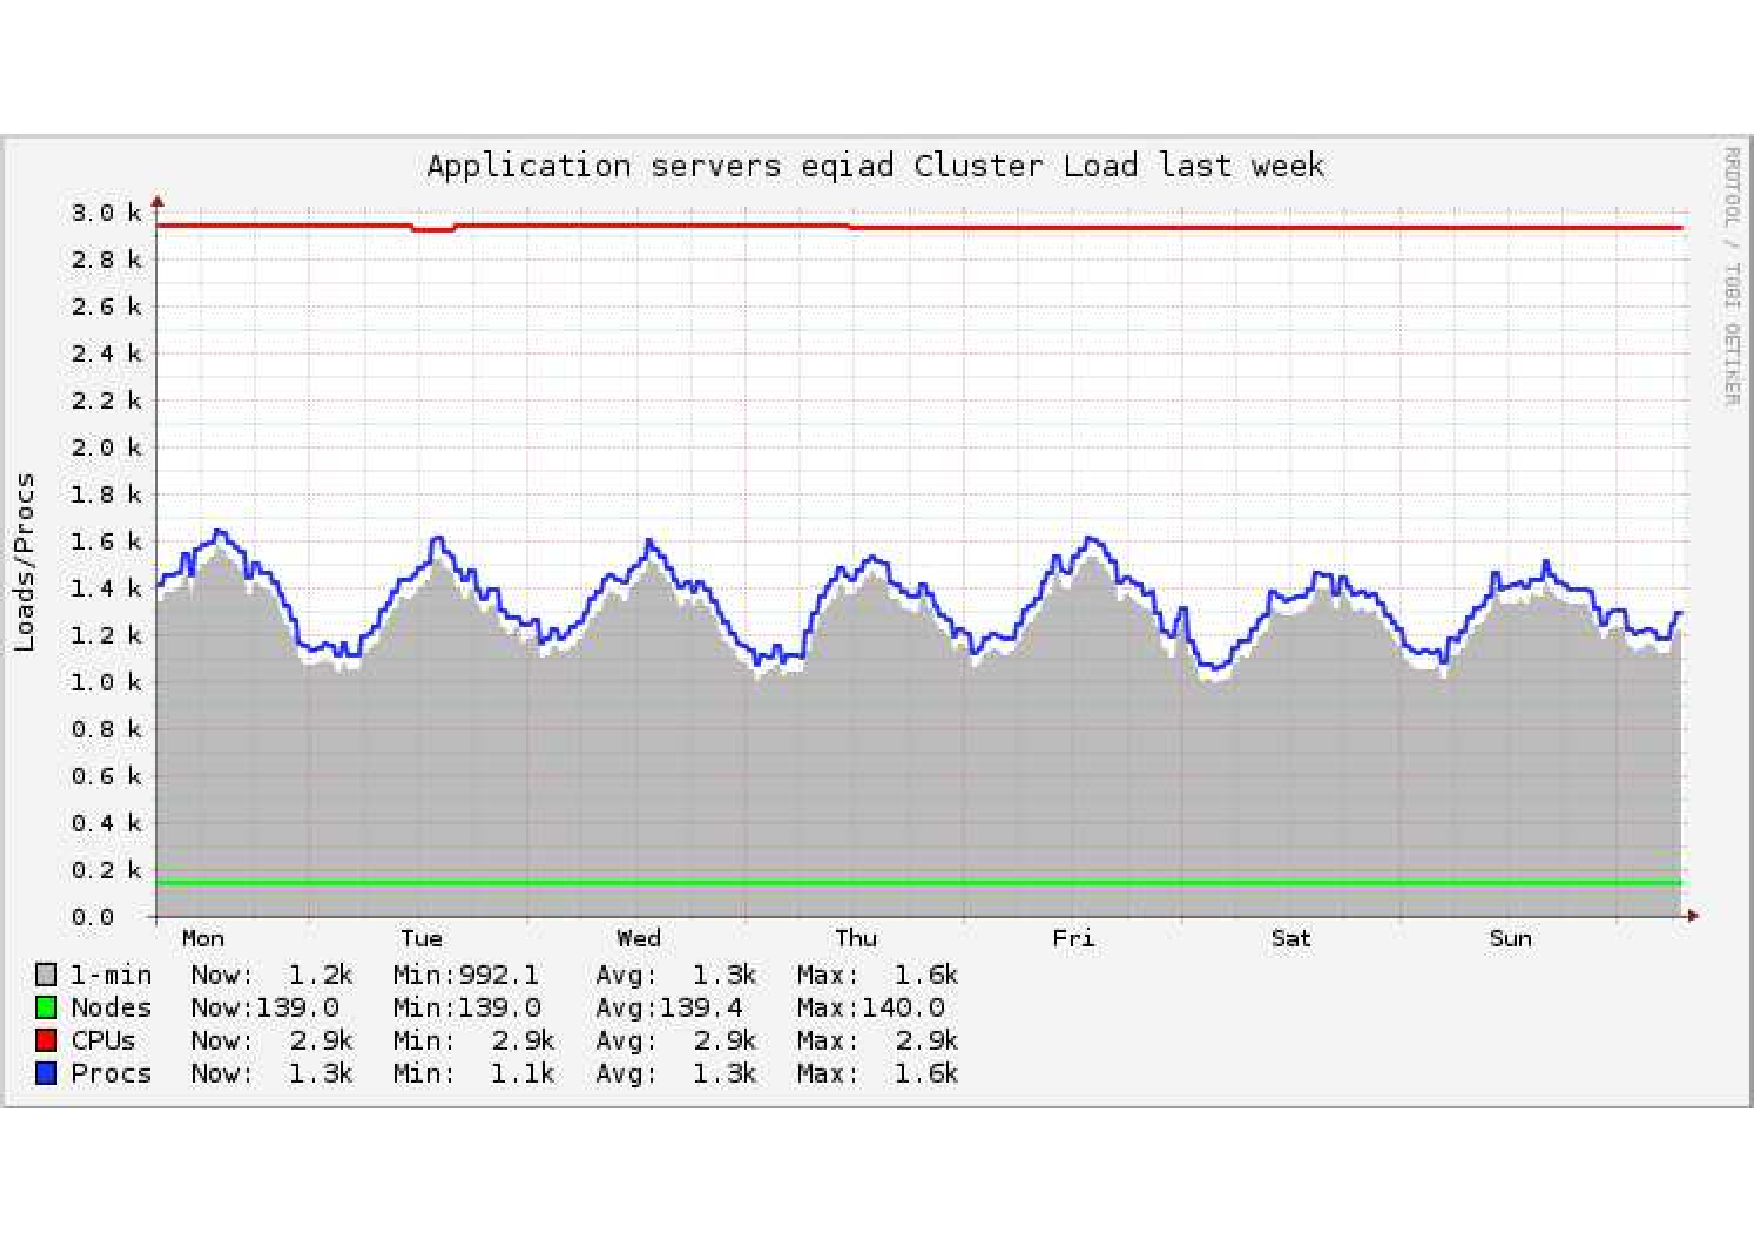
\includegraphics[width=\textwidth,keepaspectratio]{Figures/QueueingTheory/ganglia_app_server_18to24_Aug_2014.pdf}
\caption{Number of requests received by application servers during a week. 18-24 August 2014, Wikimedia Grid \cite{Ganglia_Wikimedia_Grid_Report} .}
\label{fig:ganglia_app_server_18to24_Aug_2014}
\end{figure}

\begin{figure}[!htbp]
\centering
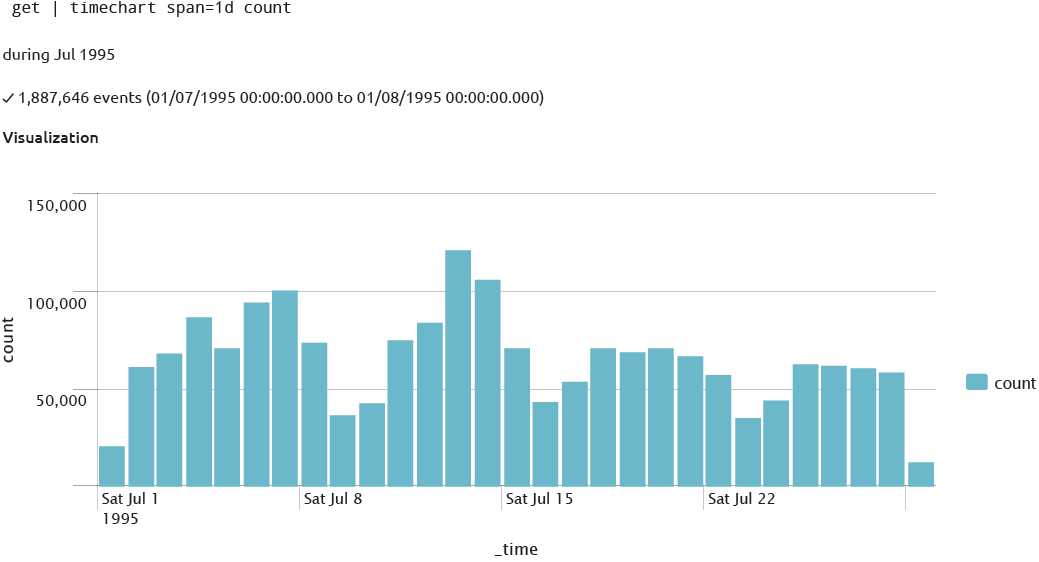
\includegraphics[width=\textwidth,keepaspectratio]{Figures/QueueingTheory/get.png}
\caption{Number of GET requests received by day \cite{plotly_ClarkNet-HTTP_get}, \cite{ClarkNet-HTTP}.}
\label{fig:_ClarkNet-HTTP_get}
\end{figure}

Incoming request rate in this workload varies depending on the day of the
week and the hour of the day. In our version of the
traces, there is a 12-hour difference between the peak (at noon)
and the trough (at midnight) in number of arriving requests, see Fig \ref{fig:ganglia_app_server_18to24_Aug_2014}.

In the simulation, random requests are generated according to:
\begin{equation}\label{eq:web_workload}
r = R_{min} + 0.5(R_{max} - R_{min}) + 0.5(R_{max} - R_{min}) sin(\frac{\pi t}{86400}) 
\end{equation}

Where 86400 is the number of seconds in a day (24 hours). $R_{max}$ is the maximum number of requests per second on that day, $R_{min}$ is the minimum number of requests of the day.

\subsubsection{Using the CloudHarmony API}

The CloudHarmony API provides an API for accessing different benchmark results for a
range of cloud services [18]. The two relevant API endpoints are:
\begin{lstlisting}
https://www.cloudharmony.com/ws/getServicesWithBenchmark
benchmarkId
https://www.cloudharmony.com/ws/getServerBenchmarkResults
benchmarkId
serverId
lastBenchmarksOnly
\end{lstlisting}

The first endpoint lists the available cloud services (and cloud servers) that have been
benchmarked with the benchmarkId (mysql-bench:select and mysql-bench:insert), and the
second endpoint retrieves the benchmark results for all the cloud servers that are passed as the
query parameters. Since we need the latest benchmark result, we also include the
‘lastBenchmarksOnly’ parameter in the query string. The API returns a JSON response that
can be parsed and utilised.

\subsection{Result}


\subsection{Database}

The mysql-bench benchmark suite is meant to tell any user what operations a given SQL implementation performs well or poorly. This benchmark is single-threaded, so it measures the minimum time for the operations performed. It measures the average time (in wallclock seconds) it takes for all of the mysql-bench benchmarks: alter-table, ATIS, big-tables, connect, create, insert, select, transactions and wisconsin. mysql-bench comprises of the following benchmarks:


\begin{enumerate}
  \item mysql-bench ATIS
  \item mysql-bench alter-table
  \item mysql-bench big-tables
  \item mysql-bench connect
  \item mysql-bench create
  \item mysql-bench insert
  \item mysql-bench select
  \item mysql-bench Wisconsin 
\end{enumerate}


In order to use these benchmark results to make useful decisions, we focus on the 2 most important query types – SELECT (READ) and INSERT (WRITE).The mysql-insert benchmark, at it’s core, issues 300,000 INSERT queries (if configured to run under default conditions) and calculates the total wall clock seconds to execute all queries. Thus if the wallclock seconds is, say t, on a particular system, we can deduce that the service rate of that server to process insert queries is $ \mu_w = \frac{300000}{t_w} $ queries/second. Similarly we can deduce the service rate for SELECT queries as $ \mu_r = \frac{1,194,631}{t_r} $ where the SELECT queries include the WHERE clause and thus SELECT queries with range parameters have been taken into account. This implies that if the fraction of READ/WRITE requests are given as $wr$ and $ww$, we can determine the average service rate as:

\begin{equation}\label{eq:db_workload}
\mu = wr \mu_r + ww \mu_w
\end{equation}

Thus using benchmark results and the READ/WRITE ratio, the service rate of different servers for performing MySQL queries can be computed.







\chapter{System Implementation and Evaluation}
\label{cha:system}
As we proposing methods to address different aspects of the research problems listed in Section \ref{sec:research_problem}, we implemented the partial solutions with some GUI and API, they can be used separately to solve each problem.
It's possible to integrate all components into one holistic framework, but since later parts were developed with more advanced technologies, integrating with older implementations makes it inefficient. So we presented those solutions as it is.

\section{CoCoOn Websites and Services}
\label{sec:cocoonImplementation}
This data model has evolved over time with the Cloud Service landscape.
We started the model with taxonomy definitions of Cloud terminologies,
see Section \ref{sec:cocoon0.1}.
Then we extended part of the ontology and developed it into
a the current version 1.0, see Section \ref{sec:cocoon1.0.1}.

The details of CoCoOn is described in Chapter \ref{cha:cocoon}. This section will explain how to use and make extension to the ontology, including: How are the ontologies, documentation, datasets hosted? How data can be collected and transformed with this ontology? How to query the result with SPARQL? And some other usage cases.

\subsection{Ontology Usage Cases}
\href{https://schema.org/}{Schema.org} does not formally include any Cloud Computing ontology yet, CoCoOn can be an extension in this area.
Its intended usage is illustrated in Figure \ref{fig:cocoon_workflow}.

\begin{figure}[!ht]
  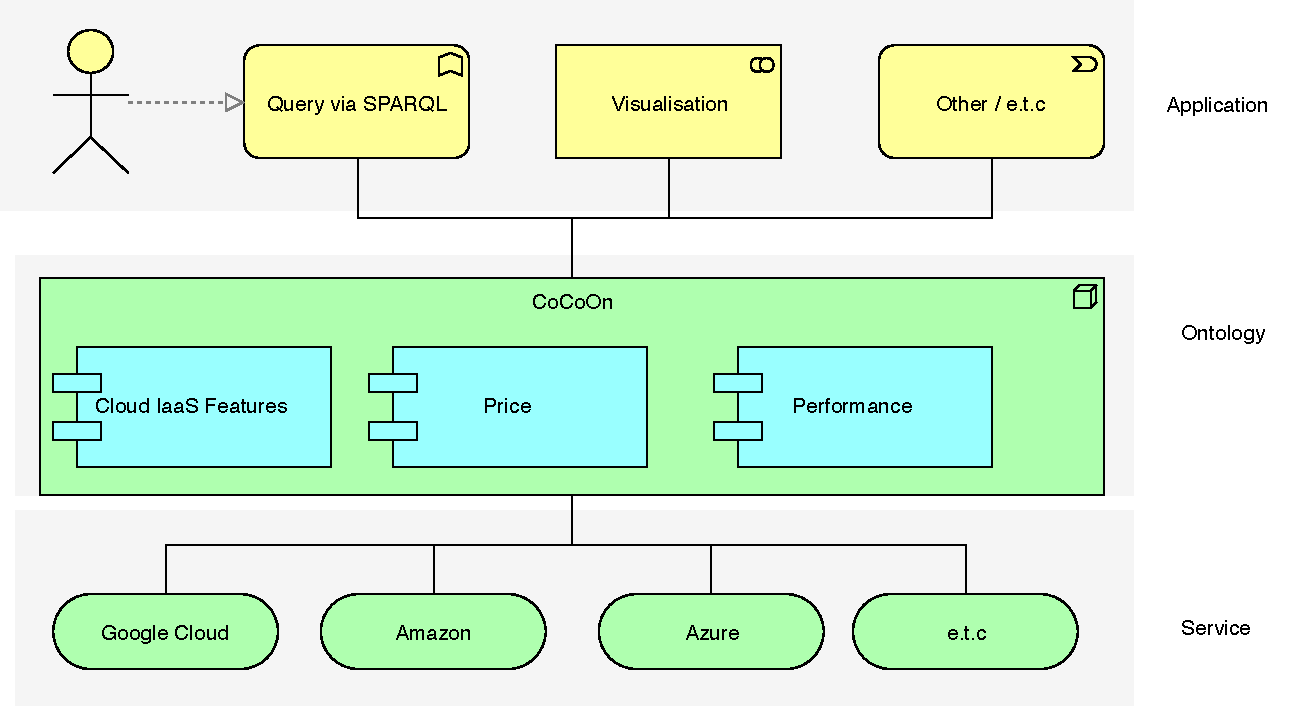
\includegraphics[width=\textwidth,keepaspectratio]{Figures/system/cocoon_usecase.pdf}
  \caption{CoCoOn Workflow}
  \label{fig:cocoon_workflow}
\end{figure}

\subsection{Mapping Data to Ontology}
For converting data from various sources to semantic data,
a number of methods were explored.
Initially we tried to transform the JSON file from the Provider APIs into a JSON-LD file by adding a \texttt{@context} to it.
After \href{https://miranda-zhang.github.io/cloud-computing-schema/json-ld-macros/gcloud.html}{experimenting with JSON-LD Macros} \cite{json-ld-macros}, we realized there are many limitations.
It only works well for simple cases but it is not sufficient to cover more complex scenarios.
So we moved to use SPARQL-Generate \cite{lefrancois_eswc_2017,sparql-generate}
for defining the mappings.

\subsubsection{Data Clean Up}
A lot of the data can be obtained from provider APIs,
in JSON or JS format.
We then clean up/transform such data with \href{https://stedolan.github.io/jq/}{jq}.
Next we mapped the cleaner data to ontologies,
and get results in RDF turtle format.

An example jq script transforms
\href{https://cloudpricingcalculator.appspot.com/static/data/pricelist.json}{json data from Google API}
is illustrated in Listing \ref{lst:jqScriptTransformsDataFromGoogleAPI}.
The \href{https://github.com/miranda-zhang/cloud-computing-schema/blob/master/example/gcloud/compute.md}{complete process with input and output} for each step is documented online with more details.

% I don't have a syntax highlighting setting for jq, so just used bash.
\begin{lstlisting}[caption={jq script transforms data from Google API},label={lst:jqScriptTransformsDataFromGoogleAPI},language=bash]
.gcp_price_list | . |=with_entries(select(.key| contains("VMIMAGE") )) | 
[ to_entries[] | 
    {
        "name": .key,
        "cores":(
            if (.key|contains("F1-MICRO")) then
                0.2 
            elif (.key|contains("G1-SMALL")) then
                0.5
            else .value.cores end
        ),
        "memory": .value.memory,
        "gceu": (
            if .value.gceu == "Shared CPU, not guaranteed" then
                null
            else .value.gceu end
        ),
        "maxNumberOfPd": .value.maxNumberOfPd,
        "maxPdSize": .value.maxPdSize,
        "price": 
         [ 
            .value | del(
                .cores, .memory, .gceu,
                .fixed, .maxNumberOfPd, .maxPdSize, .ssd)
            | to_entries[] | { "region": .key, "price": .value }
         ] 
    } 
]
\end{lstlisting}

\subsubsection{Annotating Plain Data with CoCoOn}
An example SPARQL-Generate script maps 
\href{https://azure.microsoft.com/api/v2/pricing/managed-disks/calculator/?culture=en-au&discount=mosp}{json data from Azure API about managed-disks}
to CoCoOn v1.0.1 is illustrated in Listing \ref{lst:rqgScriptAzureManaged-disks}.
The \href{https://github.com/miranda-zhang/cloud-computing-schema/blob/master/example/azure/storage.md}{complete process with input output} for each step is documented online with more details.

\begin{lstlisting}[caption={SPARQL-Generate script maps json data to ontologies},label={lst:rqgScriptAzureManaged-disks},language=sparql]
BASE <https://w3id.org/cocoon/data/v1.0.1/>
PREFIX iter: <http://w3id.org/sparql-generate/iter/>
PREFIX fun: <http://w3id.org/sparql-generate/fn/>
PREFIX rdfs: <http://www.w3.org/2000/01/rdf-schema#>
PREFIX xsd: <http://www.w3.org/2001/XMLSchema#>
PREFIX gr: <http://purl.org/goodrelations/v1#>
PREFIX cocoon: <http://w3id.org/cocoon/v1.0.1#>
PREFIX schema: <https://schema.org/>
PREFIX unit: <http://qudt.org/1.1/vocab/unit#>

GENERATE { 
  ?iri a cocoon:NetworkStorage;
    rdfs:label ?name;
    schema:dateModified ?date;
    cocoon:hasProvider ?provider;
    
    GENERATE {
        ?iri gr:hasPriceSpecification [ 
            a gr:CloudServicePriceSpecification ; 
                gr:hasCurrency "USD"^^xsd:string; 
                gr:hasCurrencyValue ?value;
                gr:hasUnitOfMeasurement cocoon:GBPerMonth ;
                cocoon:inRegion <Region/{?provider_slug}/{?region}>;
        ]
    }
  	ITERATOR iter:JSONListKeys(?prices) AS ?region
    WHERE {
        FILTER( ! CONTAINS(?managed_disk,"ultrassd") )
        BIND (xsd:float( fun:JSONPath(?prices,"$.['{?region}'].value") ) AS ?value )
    } .

    GENERATE {
        ?iri
        cocoon:hasStorageIOMax [
            a schema:TypeAndQuantityNode;
                schema:amountOfThisGood ?iops;
                schema:unitCode cocoon:IOPs;
        ];
        cocoon:hasStorageSize [
            a schema:TypeAndQuantityNode;
                schema:amountOfThisGood ?size;
                schema:unitCode cocoon:GB;
        ];
        cocoon:hasStorageThroughputMax [
            a schema:TypeAndQuantityNode;
                schema:amountOfThisGood ?speed;
                schema:unitCode unit:MegabitsPerSecond ;
        ];
    } WHERE {
        BIND (xsd:nonNegativeInteger( fun:JSONPath(?managed_disk_json,"$.iops") ) AS ?iops )
        BIND (xsd:nonNegativeInteger( fun:JSONPath(?managed_disk_json,"$.size") ) AS ?size)
        BIND (xsd:nonNegativeInteger( fun:JSONPath(?managed_disk_json,"$.speed") ) AS ?speed)        
        FILTER( BOUND(?iops) )
        # either ?iops ?size ?speed are all bound or non is bound
    } .

    GENERATE {
        ?iri
            gr:hasPriceSpecification <{?updated}/CloudStorageTransactionsPriceSpecification/{?provider_slug}/managed_disk/transactions-{?type}>;
    } WHERE {
        FILTER( ! CONTAINS(?managed_disk,"snapshot") && ! CONTAINS(?managed_disk,"ultrassd"))
        FILTER( CONTAINS(?managed_disk,"hdd") || CONTAINS(?managed_disk,"ssd") )
        BIND ( IF( CONTAINS(?managed_disk,"hdd") , "hdd" ,"ssd" ) AS ?type )        
    } .

    GENERATE {
        ?iri
            cocoon:canHaveSnapshot <{?updated}/NetworkStorage/{?provider_slug}/standardssd-snapshot>;
            cocoon:canHaveSnapshot <{?updated}/NetworkStorage/{?provider_slug}/standardhdd-snapshot-lrs>;
            cocoon:canHaveSnapshot <{?updated}/NetworkStorage/{?provider_slug}/standardhdd-snapshot-zrs>;
            cocoon:canHaveSnapshot <{?updated}/NetworkStorage/{?provider_slug}/{?premiumssd_snapshot}>;
    } WHERE {
        FILTER( !CONTAINS(?managed_disk,"snapshot") )
        FILTER( CONTAINS(?managed_disk,"premiumssd") || CONTAINS(?managed_disk,"standardssd"))
        BIND ( IF( CONTAINS(?managed_disk, "premiumssd") , "premiumssd-snapshot" , ?undefined ) AS ?premiumssd_snapshot )    
    } .

    GENERATE {
        ?iri gr:hasPriceSpecification [ 
            a gr:CloudServicePriceSpecification ;
                gr:hasCurrency "USD"^^xsd:string; 
                gr:hasCurrencyValue ?value;
                gr:hasUnitOfMeasurement ?unit ;
                cocoon:inRegion <Region/{?provider_slug}/{?region}>;
                rdfs:label ?label;
        ].
    }
  	ITERATOR iter:JSONListKeys(?prices) AS ?region
    WHERE {
        FILTER( CONTAINS(?managed_disk,"ultrassd") ) 
        BIND (xsd:float( fun:JSONPath(?prices,"$.['{?region}'].value") ) AS ?value )
        BIND (
            COALESCE(
                IF(CONTAINS(?managed_disk,"iops"), cocoon:IOPsPerHour, 1/0),
                IF(CONTAINS(?managed_disk,"stored"), cocoon:GBPerHour, 1/0),
                IF(CONTAINS(?managed_disk,"throughput"), cocoon:MegabitsPerSecondPerHour, 1/0),
                cocoon:VcpuPerHour # assume "vcpu"
            ) AS ?unit
        )
        BIND ( STRAFTER(?managed_disk,"-") AS ?label)      
    } .
}
SOURCE <https://raw.githubusercontent.com/miranda-zhang/cloud-computing-schema/master/example/jq/azure/2019-03-07/managed-disks.json> AS ?source
ITERATOR iter:JSONListKeys(?source) AS ?managed_disk
WHERE {
    BIND (fun:JSONPath(?source,"$.['{?managed_disk}']") AS ?managed_disk_json)
    BIND (fun:JSONPath(?managed_disk_json,"$.prices") AS ?prices)
    # having signle point of change for the following
    BIND ( "Azure" as ?provider_slug )
    BIND ( cocoon:Azure as ?provider )
    BIND ( "2019-03-07" as ?updated) # yr-month-day
    BIND ( xsd:date(?updated) as ?date )
    BIND ( IF (CONTAINS(?managed_disk,"ultrassd"), "ultrassd", ?managed_disk) AS ?name )
    BIND ( <{?updated}/NetworkStorage/{?provider_slug}/{?name}> AS ?iri )
}
\end{lstlisting}

\href{https://github.com/miranda-zhang/cloud-computing-schema/tree/master/example/sparql-generate}{More examples are online}. For those scripted tasks, we can automate the process, and additional information collection steps with human interpretation mostly are once off task which we have addressed with this project.

\subsubsection{Result}
We have also made the complete data-set (132,282 triples) available at
\href{https://w3id.org/cocoon/data}{https://w3id.org/cocoon/data}.
It is hosted with \href{http://linkeddatafragments.org/}{Linked Data Fragments Server} on Google Cloud.

\section{QoS Profiler}
In this section we describe the implementation of this QoS profiler proposed in Section \ref{sec:qos}.

\subsection{QoS Data Collection Scripts}
Data is collected from \href{https://cloudharmony.com}{CloudHarmony}, initially we used the HtmlUnit library \cite{htmlunit}.

Later as CloudHarmony evolves, we also upgraded our script.
\href{https://github.com/miranda-zhang/cloud-computing-schema/tree/master/example/cloudharmony}{More technical details on measuring QoS} is documented online. We also provided live demos of QoS tests, e.g.
\href{https://miranda-zhang.github.io/cloud-computing-schema/cloudharmony/google/test.html}{Downlink Speed and Latency tests for Google Cloud Services}.
\href{https://github.com/miranda-zhang/cloud-computing-schema/blob/master/example/cloudharmony/selenium/cloudharmony.py}{Uplink tests scripts are written in python}
as \href{https://github.com/miranda-zhang/cloud-computing-schema/tree/master/example/cloudharmony/selenium}{selenium} is required.

\subsection{Distributed Archetecture}
Fig. \ref{fig1} shows the top level dataflow of the system we implemented.

\begin{figure}[!ht]
 \centering
 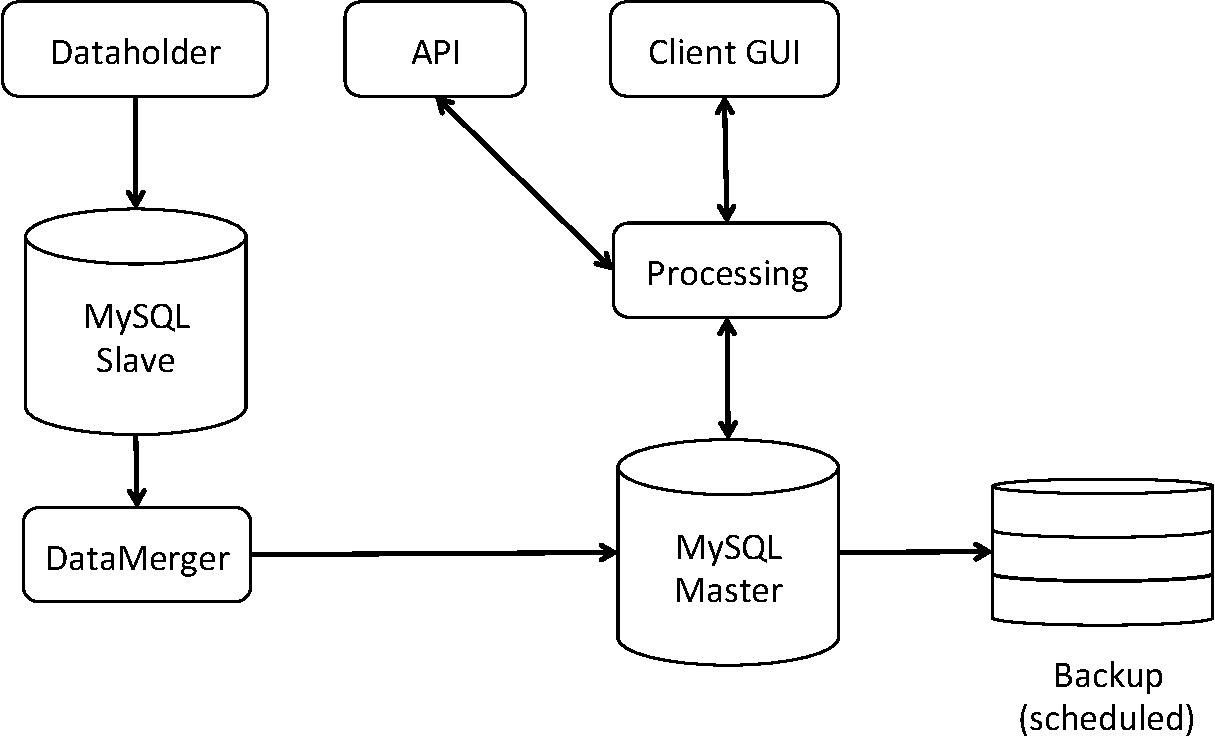
\includegraphics[width=\textwidth,keepaspectratio]{Figures/QoS/figure1.pdf}
 \caption{Abstract System Dataflow. This figure is better looking together with Fig. \ref{fig:QoSMonitoringServiceNetworkTopology} for better understanding. As we have used several (slave) servers to collect data from different locations. Then we transfer them to a central server for processing and backup, data on this server was also archived and cleared manually every time after we imported the newly collected data into the local offline system for post-processing and cleaning up. We only use the (summarised) average QoS data for real time querying via API and web GUI, as this allows us to provide response faster.}
\label{fig1}
\end{figure}

Fig. \ref{fig3} shows the overview of our system architecture. We use Dropbox as the backup service for this prototype implementation to demonstrate the feasibility. As long as data is properly backed up in a separate location, other mechanisms can be used, i.e. git repository.

\begin{figure}[!ht]
 \centering
 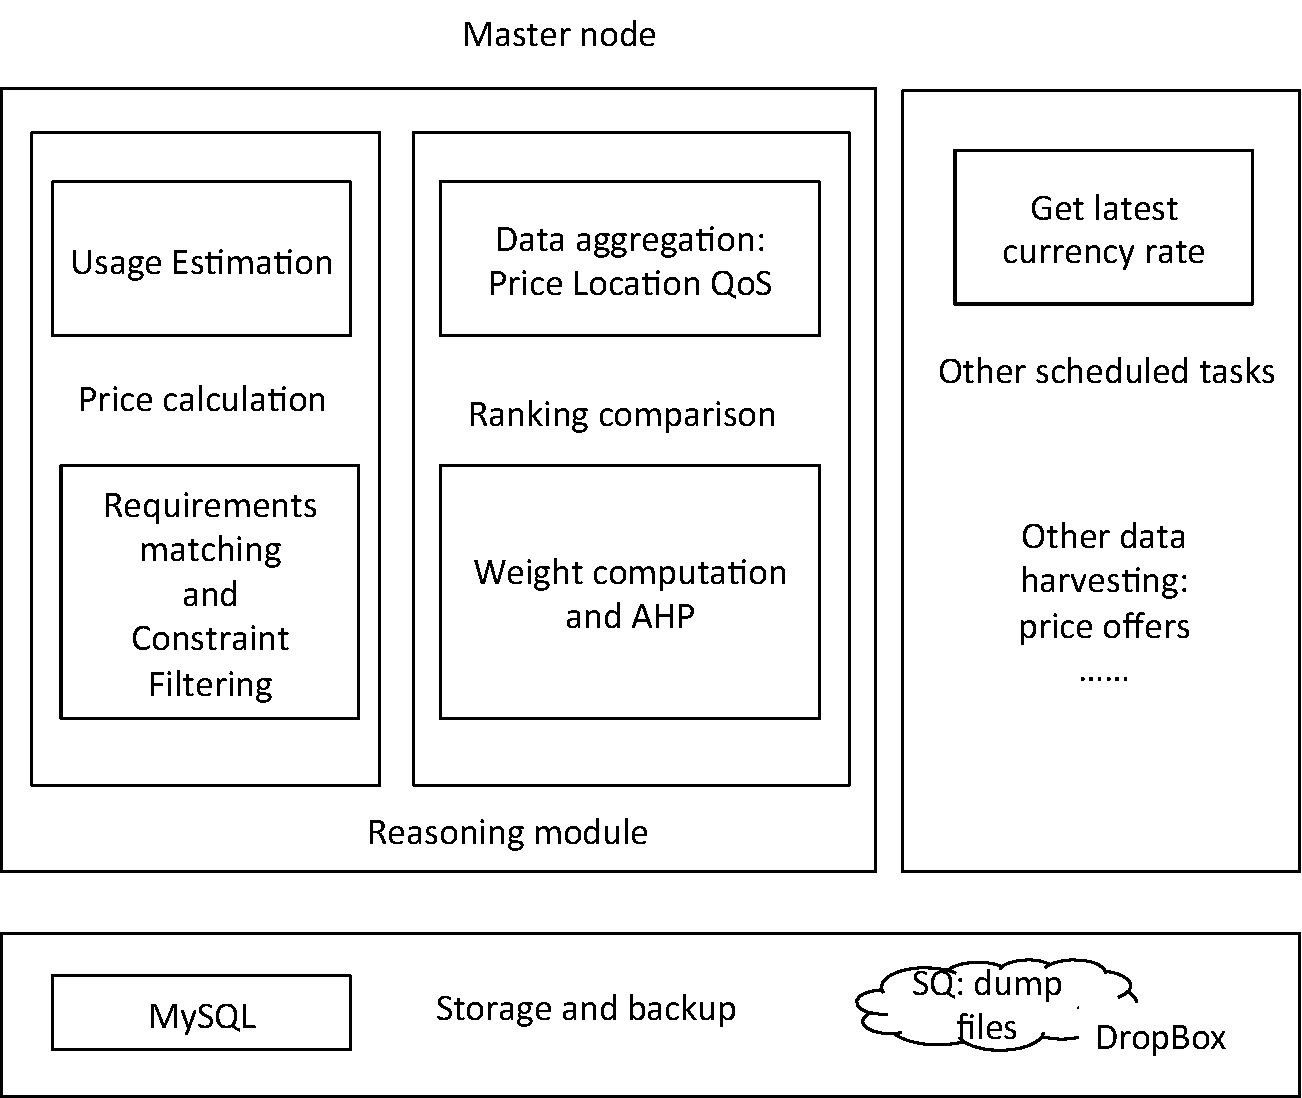
\includegraphics[width=\textwidth,keepaspectratio]{Figures/QoS/figure3.pdf}
 \caption{Master Node System Architecture. In the reasoning module main functions and operations are broke down into different blocks. There are some other tasks cannot be strictly categorized into existing modules, those are put into the ``Other Tasks" section, and the very light grey block contains the evolving part of the system so it cannot be considered a stable component of the system. While it’s possible to backup the whole server, it is not necessary at this stage, and the most valuable data is stored in the MySQL database, which can be backuped much easier and cheaper by creating ``SQL dump". This dump file is created daily and simply stored in a Dropbox folder which is free to use and keeps a history of the file stored in it for 30 days, which is sufficient for our case. The presentation layer (UI and API implementation) and monitoring module are omitted to keep the diagram simple.}
\label{fig3}
\end{figure}

The price data is collected from providers' websites. The problem with automatic data collection can be solved if providers release more structured data with sufficient metadata description, we have proposed an ontology in Chapter \ref{cha:cocoon}.

\section{CloudRecommender}
\label{sec:CloudRecommender}
Despite the popularity of Cloud Computing, existing Cloud Service manipulations (e.g. select, start, stop, configure, delete, scale and de-scale) techniques require human familiarity with different Cloud service types and typically rely on procedural programming or scripting languages. The interaction with services is performed through low-level application programming interfaces (APIs) and command line interfaces. This is inadequate, given the proliferation of new providers offering services at different layers (e.g. SaaS, PaaS, and IaaS). One of the consequences of this state is that accessibility to Cloud Computing is limited to decision makers with IT expertise. This raises a set of research questions: How to develop interfaces that can transform low, system-level programming to easy-to-use drag and drop operations? Will such interfaces improve and simplify the process of Cloud Service Selection and Comparison?

Therefore, we present CloudRecommender, a decision support system, using transactional SQL semantics, procedures and views. The benefits to users of CloudRecommender include, for example, the ability to estimate costs, compute cost savings across multiple providers with possible tradeoffs and provide visual aid in the selection of Cloud services.

\subsection{Related Work}
Prior to CloudRecommender, there have been a variety of systems that use declarative logic-based techniques for managing resources in distributed computing systems. The focus of the authors in work \cite{Liu2011} is to provide a distributed platform that enables Cloud providers to automate the process of service orchestration via the use of declarative policy languages.
The authors in \cite{Brodsky2009} present an SQL-based decision query language for providing a high-level abstraction for expressing decision guidance problems in an intuitive manner so that database programmers can use mathematical programming technique without prior experience.
We also draw inspiration from the work in \cite{DBLPconfCIDRMaoLMF11} which proposes a data-centric (declarative) framework to improve SLA fulfillment ability of Cloud service providers by dynamically relocating infrastructure services.
COOLDAID \cite{Chen2010} presents a declarative approach to manage configuration of network devices and adopts a relational data model and Datalog-style query language.
NetDB \cite{Caldwell2004} uses a relational database to manage the configurations of network devices. However, NetDB is a data warehouse, not designed for Cloud service selection or comparison. However, NetDB is a data warehouse, not designed for Cloud service selection or comparison. 

In contrast to the aforementioned approaches, CloudRecommender is designed for solving the new challenge of handling heterogeneous service configuration and naming conventions in Cloud computing. It is designed with a different application domain – one that aims to apply declarative and widget programming technique for solving the Cloud service selection problem.

\subsection{System Architecture}
The CloudRecommender system architecture consists of three layers: the configuration management layer, the application logic layer and the User interface (widget) layer.
Shown in Fig. \ref{fig:SystemDeploymentStructure}.

\begin{figure}[!ht]
  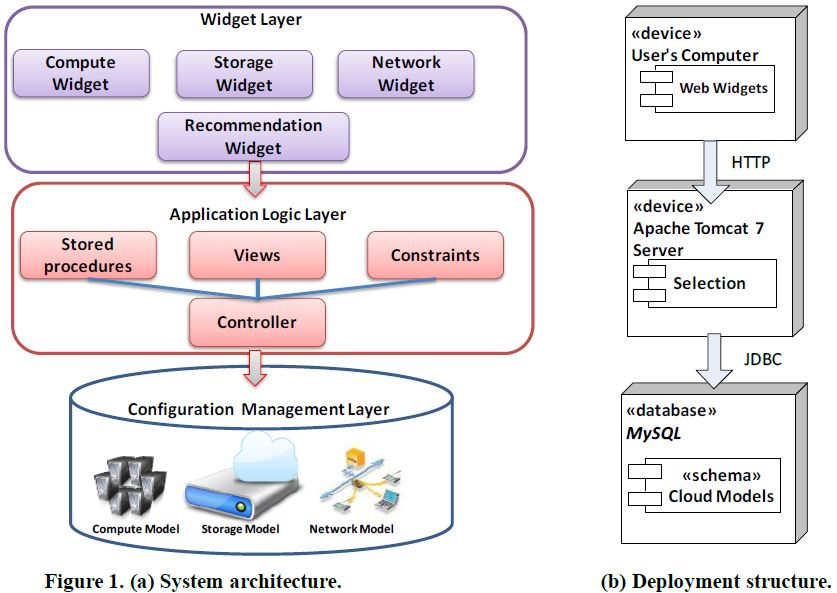
\includegraphics[width=\textwidth,keepaspectratio]{Figures/system/CloudRecommender/SystemArchitecture.jpg}
  \caption{System architecture and deployment structure}
  \label{fig:SystemDeploymentStructure}
\end{figure}

Figure \ref{fig:SystemDeploymentStructure}(b) shows the deployment structure of the CloudRecommender system.
For persistence we have chosen MySQL for its agility and popularity, but any other relational database can be plugged in. 
Furthermore, many APIs provided by cloud
providers (such as Amazon) and open source cloud management frameworks (e.g.
jclouds) are written in Java. Thus, Java is chosen as the preferred language to
implement the application logic layer to ease the integration with external libraries.

The configuration layer maintains the basic cloud domain model related to compute, storage, and network services.
Initially we stored recommender system data into a relational database,
its implementation is detailed in Section \ref{sec:InfrastructureServiceConfigurationRepository}.
But as we go deeper with understanding of the Cloud domain,
we increasing find this database model is hard to update,
thus hard to keep up to date with rapid changing Cloud services,
and not very readable to whom do not have knowledge of our recommender system,
as the database schema designed to be optimal for recommendation service with unique table structure and procedures.
So later, we developed the Cloud Computing Ontology (CoCoOn) model with OWL.
See Chapter \ref{cha:cocoon}.
The later proposed model is flexible and extensible enough to accommodate new services with minimal changes to our implementation. 

\subsubsection{Configuration Management Layer}
\label{sec:InfrastructureServiceConfigurationRepository}
The repository of available infrastructure services from different
providers consists data of compute, storage and network services.
These infrastructure services have very different configurations and pricing models, see Section \ref{sec:TheProblemOfSelectingOptimalServiceConfiguration} for some examples.
We collected service configuration information from a
number of public cloud providers (e.g., Windows Azure, Amazon, GoGrid,
RackSpace, Nirvanix, Ninefold, SoftLayer, AT and T Synaptic, Cloud Central, etc.) to demonstrate the generic nature of the domain model with respect to capturing heterogeneous configuration information of infrastructure services. 

We formally capture the domain knowledge (e.g., IaaS configurations)
using a declarative logic-based language, and then apply the
knowledge on top of relational data model that encapsulates
Cloud-wide information. Based on this knowledge, we have
drawn the relationships in the conceptual IaaS configuration
model and represented in Fig. \ref{fig:uml}.

Relationships between concepts representing services are carefully considered and normalized to avoid update anomalies. Services from various providers often have very different configurations and pricing models. Distinct and ambiguous
terminologies are often used to describe similar configurations.
Regardless of how providers name their services, we categorize infrastructure services based on their basic functionality.
Unit conversions were performed during instantiation of concepts.

The choice of a relational model and SQL as query language was made because of the convenience SQL procedures offers us in regards to defining templates for a given widget type. We use stored procedures to create temporary tables and to concatenate parameters to dynamically generate queries based on the user input.

\begin{figure}
  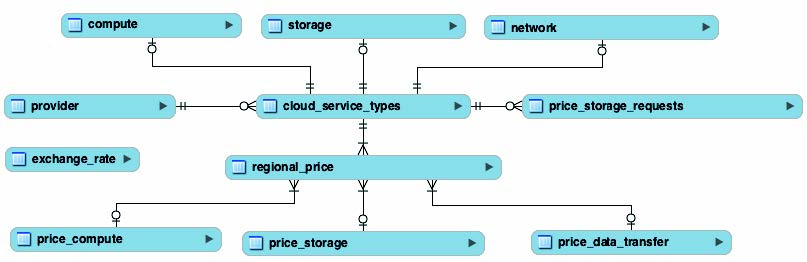
\includegraphics[width=\textwidth,keepaspectratio]{Figures/system/CloudRecommender/uml.jpg}
  \caption{Conceptual UML data model representing infrastructure service entities and their relationships}
  \label{fig:uml}
\end{figure}

For providers that offer different regional prices, we store the location information in the price table.
If multiple regions have the same price, we choose to combine them.
In the database version implementation, any changes to existing configurations (such as updating memory size, storage provision etc.) of services can be done by executing customized update SQL queries.

We have applied declarative service
selection technique by utilizing SQL and regular expressions
minimize side effects and reinforce constrains. Thus, leading
to a improved Cloud service representation and selection.

The service selection logic developed by our research is
transactional and applies well-defined SQL semantics for
querying, inserting, and updating IaaS configurations. In
addition, the proposed declarative approach is preferable
over hard coding the sorting and selection algorithm (as used
in \cite{Ruiz-AlvarezCloudStorageSelection})
as it allows us to take the advantage of optimized
query operations (e.g. select and join). 

The problem we are
trying to solve involves computing the Cartesian product
O(N * M) of multiple sets of options. A widely used solution
of such operation is the JOIN operation in database. Note
that much work in database-systems has aimed
at efficient implementation of joins. In fact, modern database
often use HASH JOIN O(N + M) and MERGE JOIN
O(N*Log(N) + M*Log(M)). They are much faster than O(N
* M).

\subsubsection{Application Logic Layer}
The request for service selection in CloudRecommender is expressed as SQL queries.
The selection process supports an application logic that builds upon the following declarative constructs: criterion, views and stored procedures. The CloudRecommender builds upon SQL queries which are executed on top of the relational data model.

\textbf{Criterion:} Criterion is a quantitative or qualitative bound (minimum, maximum, equal) on the configuration parameters provided by a service. Cloud services’
configuration parameters and their range/values listed in
Table \ref{table:IaaSConfigurations} form the basis for
expressing selection goal and criteria (e.g., select a cheapest (goal) compute service where (criterion) 0<Ram<=20, 0<=local storage<=2040, number of hours to be used per month = 244). 
An example query is shown below in Fig. \ref{fig:ExampleQueryProcedure}:

\begin{table}
\begin{tabular}{|l|p{5.5cm}|p{5.5cm}|}
\hline
Service                  & Configurations Parameters                                         & Range/possible values                                         \\ \hline
\multirow{9}{*}{Compute} & Core                                                              & >=1                                                           \\ \cline{2-3} 
                         & CPUClockSpeed                                                     & >0                                                            \\ \cline{2-3} 
                         & hasMemory                                                         & >0                                                            \\ \cline{2-3} 
                         & hasCapacity                                                       & >=0                                                           \\ \cline{2-3} 
                         & Location                                                          & North America, South America, Africa, Europe, Asia, Australia \\ \cline{2-3} 
                         & CostPerPeriod                                                     & >= 0                                                          \\ \cline{2-3} 
                         & PeriodLength                                                      & >0                                                            \\ \cline{2-3} 
                         & CostOverLimit                                                     & >= 0                                                          \\ \cline{2-3} 
                         & PlanType                                                          & Pay As You Go, Prepaid                                        \\ \hline
\multirow{7}{*}{Storage} & StorageSizeMin                                                    & >= 0                                                          \\ \cline{2-3} 
                         & StorageSizeMax                                                    & > 0                                                           \\ \cline{2-3} 
                         & CostPerPeriod (e.g. Period = Month) (e.g. UnitOfMeasurement = GB) & >= 0                                                          \\ \cline{2-3} 
                         & Location                                                          & North America, South America, Africa, Europe, Asia, Australia \\ \cline{2-3} 
                         & RequestType                                                       & put, copy, post, list, get, delete, search                    \\ \cline{2-3} 
                         & CostPerRequest                                                    & >= 0                                                          \\ \cline{2-3} 
                         & PlanType                                                          & Pay As You Go, Prepaid, Reduced Redundancy                    \\ \hline
\multirow{2}{*}{Network} & CostDataTransferIn                                                & >=0                                                           \\ \cline{2-3} 
                         & CostDataTransferOut                                               & >=0                                                           \\ \hline
\end{tabular}
\caption{Infrastructure service types and their configurations}
\label{table:IaaSConfigurations}
\end{table}

\begin{figure}
  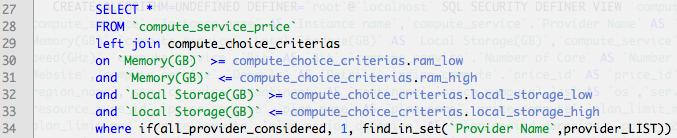
\includegraphics[width=\textwidth,keepaspectratio]{Figures/system/CloudRecommender/sql.jpg}
  \caption{Example query in procedure.}
  \label{fig:ExampleQueryProcedure}
\end{figure}

\textbf{Procedures:} We have implemented a number of customized procedures that automate the service selection process. A number of routines are prepared to process a user service selection request. List of inputs are stored in a temporary table to be passed into the procedures. As such, the size of the input list can be very long.
Final results are also stored in temporary tables, which are automatically cleared after the expiration of user session.

\textbf{Controller:} The controller supports enforcement of criteria and dynamically generates SQL queries which fulfill a given selection preference stated by the user.
Due to space considerations we are not able to depict the complete algorithm, but Fig. \ref{fig:SelectionLogic} shows the selection logic in a simplified diagram. Next we explain the basic
steps which are executed for resolving a service selection request.

\begin{figure}
  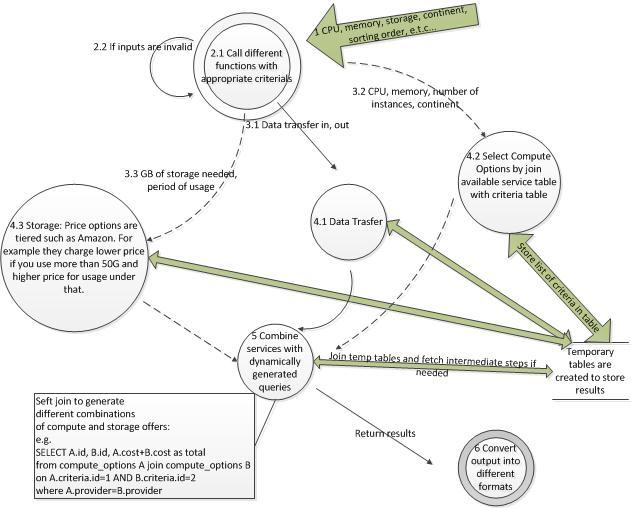
\includegraphics[width=\textwidth,keepaspectratio]{Figures/system/CloudRecommender/SelectionLogic.jpg}
  \caption{Service Selection logic.}
  \label{fig:SelectionLogic}
\end{figure}

\begin{enumerate}
    \item Basic validation is preformed on user inputs at the controller, appropriate errors are returned accordingly.
    \item Depending on user’s requirements, process 3.2 or 3.3 may not happen. This is why they are shown as dotted lines, i.e. user can query storage or compute only IaaS services. But data transfer parameters have to be set, as user will definitely transfer data in and out of the compute or storage service.
    \item Multiple temporary tables are created during the process so intermediate results (i.e. selection details of the final recommendation) can be fetched later as needed.
    \item It is possible for a user to choose multiple compute services each with different criteria. (E.g. they may have 10 set of requirements, and choose 10 instances for each.) So in process 5, query with different number of join operations are dynamically constructed.
    \item Currency conversions are performed before costs are compared.
\end{enumerate}

\textbf{Computational Complexity of Service Selection Logic}:
For a provider p, suppose it has r regions, v different kind of VMs,
s storage options, n network services.
There will be $r \times v$ different prices for VM, similarly for prices of storage ($r \times s$)
and network ($r \times n$).
And theoretically a total number of $r^{3} \times v \times s \times n$ possible combinations.
We can normally reduce the number of
options significantly in the early stage if a user has strict requirements. In the worst
case scenario, the logic needs to compute a full cross join (Cartesian product).

Another factor effecting the price calculation is the different price tiers for some services. 
Price tier example: AWS S3 charges 0.125 USD per GB for the first 1 TB /
month of usage, 0.093 for the next 49 TB, etc.
Depending on the estimated usage,
the larger the usage, the more price tiers will be involved.

Let us assume that each
provider offers approximately the same service in each region to simplify the
derivation of the computational complexity.

Let $cs_{p}$ be the number of compute services of provider p.
All regions are included, i.e. $cs_{p} = r \times v$.
Let $ss_{p}$ be the number of storage services, and $st_{p}$ be the number of storage service tiers,
$nt_{p}$ be the number of network service tiers,
$ns_{p}$ be the number of network services.
As such, the total number of offers can be
represented as follows:
$$
\sum_{p=1}^{P} cs_{p} \times (ss_{p} \times st_{p}) \times (ns_{p} \times nt_{p})
$$
Where P is the number of cloud providers.

The queries of the selection logic works as follows. After filtering out criteria-violating
services, resulting services are combined via JOIN operation(s) with final
costs calculated. In worst case scenario where a few or no criteria are defined, the
combination of the services is a full CROSS JOIN over all existing services.
Therefore, the selection queries, to our best knowledge,
have the upper bound computational complexity of
$$
O_{query}(\sum_{p=1}^{P}|cs_{p} c_{v} (ss_{p} st_{p} c_{s}) (ns_{p} nt_{p} c_{n}) | )
$$
where c means criteria, $c_{v}, c_{s}, c_{n}$ are criteria for compute, storage and network.
$ss_{p} st_{p}$ and $ns_{p} nt_{p}$ can be pre-computed, and stored as views.
However, in case the database system lacks
support for cached views in a worst case the effort multiplies with the effort of the
views’ JOIN. Modern database can use HASH JOIN O(N + M) and MERGE JOIN
O(N*Log(N) + M*Log(M)) which are faster than O(N * M).

\subsection{Interface: GUI and API}
The widget layer is implemented using a number of JavaScript frameworks including jQuery, ExtJS and YUI. CloudRecommender also exposes RESTful
(REpresentational State Transfer) APIs (application programming interface) that help external applications to programmatically compose infrastructure cloud services based on the CloudRecommender selection process.

\begin{figure}
  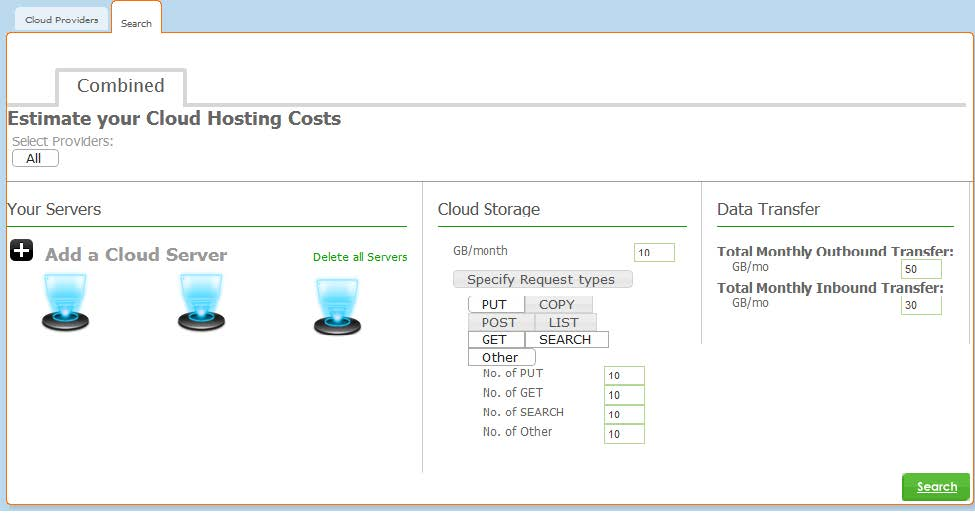
\includegraphics[width=\textwidth,keepaspectratio]{Figures/system/CloudRecommender/widget_combined.jpg}
  \caption{Screenshot of the widget combined tab.}
  \label{fig:widget_combined}
\end{figure}

\begin{figure}
  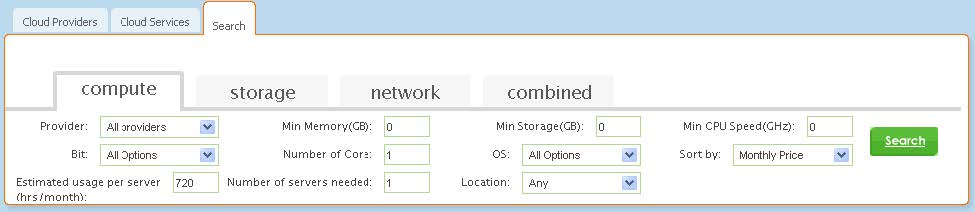
\includegraphics[width=\textwidth,keepaspectratio]{Figures/system/CloudRecommender/widget_compute.jpg}
  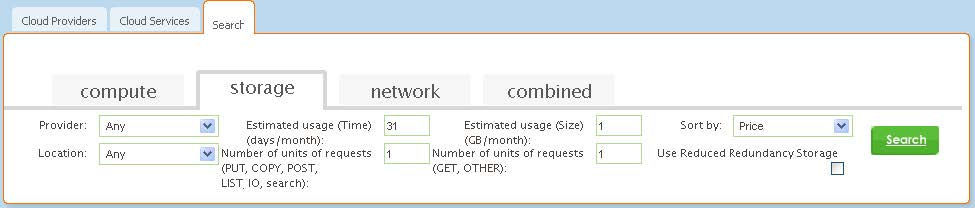
\includegraphics[width=\textwidth,keepaspectratio]{Figures/system/CloudRecommender/widget_storage.jpg}
  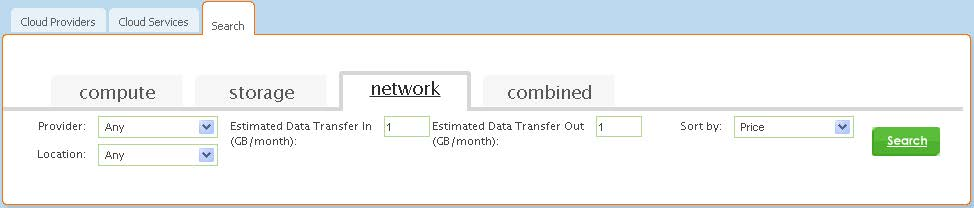
\includegraphics[width=\textwidth,keepaspectratio]{Figures/system/CloudRecommender/widget_network.jpg}
  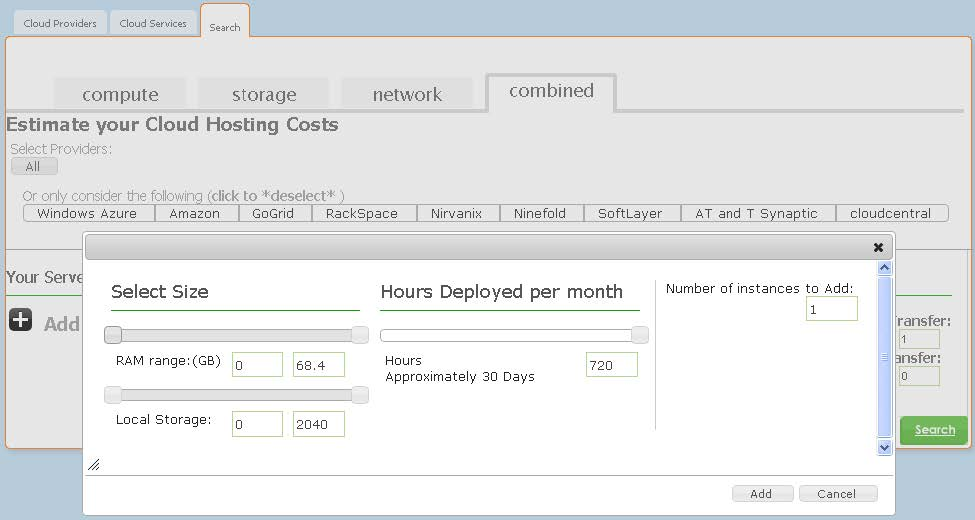
\includegraphics[width=\textwidth,keepaspectratio]{Figures/system/CloudRecommender/widget_combined_popup.jpg}
  \caption{Compute, Storage, Network and the combined service selection widgets screenshots.}
  \label{fig:widget_screenshots}
\end{figure}

This layer features rich set of user-interfaces (see Fig. \ref{fig:widget_combined}
and \ref{fig:widget_screenshots})
that further simplify the selection of configuration parameters related to cloud services.
This layer encapsulates the user interface components in the form of four principle widgets including: Compute, Storage, Network, and Recommendation. The selection of basic configuration parameters related to compute services including their RAM capacity, cores, and location can be facilitated through the Compute widget. It also allows users to search compute services by using regular expressions, sort by a specific column etc. Using the Compute widget, users can choose which columns to display and rearrange their order as well. The Storage widget allows users to define configuration parameters such as storage size and request types (e.g., get, put, post, copy, etc.). Service configuration parameters, such as the size of incoming data transfer and outgoing data transfer can be issued via the Network widget. Users have the option to select single service types as well as bundled (combined search) services driven by use cases. The selection results are displayed and can be browsed via the Recommendation widget.
See Section \ref{sec:case_studies} for some examples.

CloudRecommender also exposes REpresentational State
Transfer (RESTful) APIs that help external applications to
programmatically obtain results, i.e. recommended
infrastructure Cloud services configurations, shown in Fig. \ref{fig:REST}.

\begin{figure}[!ht]
  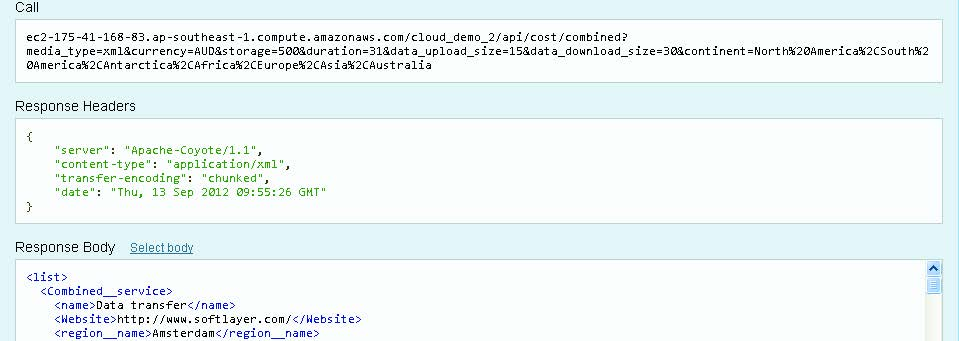
\includegraphics[width=\textwidth,keepaspectratio]{Figures/system/CloudRecommender/REST.jpg}
  \caption{REST call via HTTP GET request}
  \label{fig:REST}
\end{figure}

\subsection{Experiment}
In this section, we present the experiments and evaluation that we undertook.

\textbf{Experiment Setup:} We hosted our CloudRecommender system instance on Amazon
EC2 using a standard small instance in the US-west location. By default, the small
instance has the following hardware configuration: 1.7 GB of main memory, 1 EC2
Compute Unit, 160 GB of local instance storage, and a 32-bit platform with an
Ubuntu 10.04 operating system. We populated CloudRecommender with
infrastructure service configuration information related to Amazon, Azure, GoGrid,
RackSpace, Nirvanix, Ninefold, SoftLayer, AT and T Synaptic, and Cloud Central (an
Australian provider).

\textbf{Service Selection Test:}
\begin{figure}[!ht]
  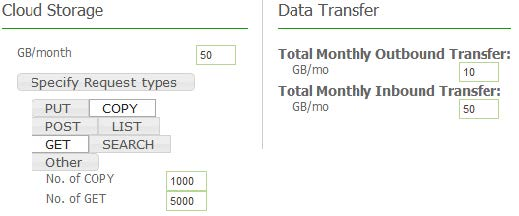
\includegraphics[width=\textwidth,keepaspectratio]{Figures/system/CloudRecommender/ServiceSelectionTestCase.jpg}
  \caption{Service selection criteria set by business analyst.}
  \label{fig:ServiceSelectionTestCase}
\end{figure}
Suppose an enterprise wants to migrate its data to the
cloud with the aim of storing and sharing it with other branches through public cloud
storage (note that security issues are dealt within the enterprise applications). At this
stage, we assume the business analyst of the enterprise has a good estimation of the
data storage and transfer (network in/network out) requirements. By using
CloudRecommender, the analyst would like to find out which of the public cloud
providers would be most cost-effective in regards to data storage and transfer costs.
For this selection scenario, the analyst inputs the following anticipated usage
information for the storage and network services: (i) Data size of 50 GB, 1000 copy
requests and 5000 get requests and (ii) data transfer in size of 10 GB and data transfer
out size of 50 GB.

As shown in Fig. \ref{fig:ServiceSelectionTestCase}, the analyst specifies service selection criteria via the storage and network widgets. Programmatically, the above request can also be submitted via the
RESTful service interface of the CloudRecommender as shown below in Fig. \ref{fig:ExampleRESTcallGET}.

\begin{figure}[!ht]
  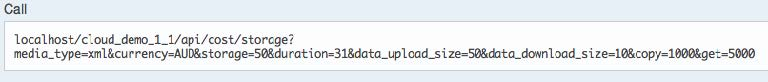
\includegraphics[width=\textwidth,keepaspectratio]{Figures/system/CloudRecommender/GET.jpg}
  \caption{An Example REST call.}
  \label{fig:ExampleRESTcallGET}
\end{figure}

Once this selection request is submitted, the controller validates and parameterizes the
criteria (user inputs). Though not shown in the above figures, the business analyst also has the
option to express whether the selection criteria should be evaluated against all the
available cloud providers or only the selected ones (e.g., Amazon, Azure, and GoGrid
only). As mentioned earlier, the application logic layer implements specialized views
and procedures for evaluating different service selection scenarios.
CloudRecommender captures and inserts multiple storage and network service
selection criteria into specialized views called "\texttt{storage\_selection\_criteria}" and
"\texttt{network\_selection\_criteria}". Aforementioned views are then joined against the
"\texttt{storage\_service\_price}" and "\texttt{network\_service\_price}" views for estimating the cost of
using the combined cloud services.

\begin{figure}[!ht]
  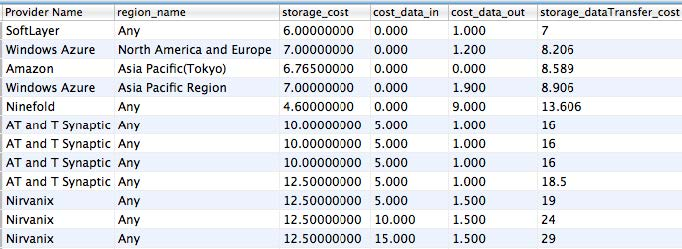
\includegraphics[width=\textwidth,keepaspectratio]{Figures/system/CloudRecommender/recommendationResults.jpg}
  \caption{Storage and network services recommendations for the business analyst selection use case.}
  \label{fig:StorageNetworkServicesRecommendations}
\end{figure}

Fig. \ref{fig:StorageNetworkServicesRecommendations} shows the result of the
selection scenario depicted in Fig. \ref{fig:ServiceSelectionTestCase}.
Results are sorted into increasing total cost order (i.e. "\texttt{storage\_dataTransfer\_cost}"
column). "Any" means the provider offers the same price for all of its regions. In the
case of SoftLayer, it charges the same price in all regions. In the case of Amazon
AWS, since it offers different prices for different regions, the enterprise may be able
to consume the same service with a cheaper price in a different region. The base
currency is USD, but since in the call the analyst had specified "currency=AUD", the
result shown is in AUD accurate to one decimal place.

\begin{figure}[!ht]
  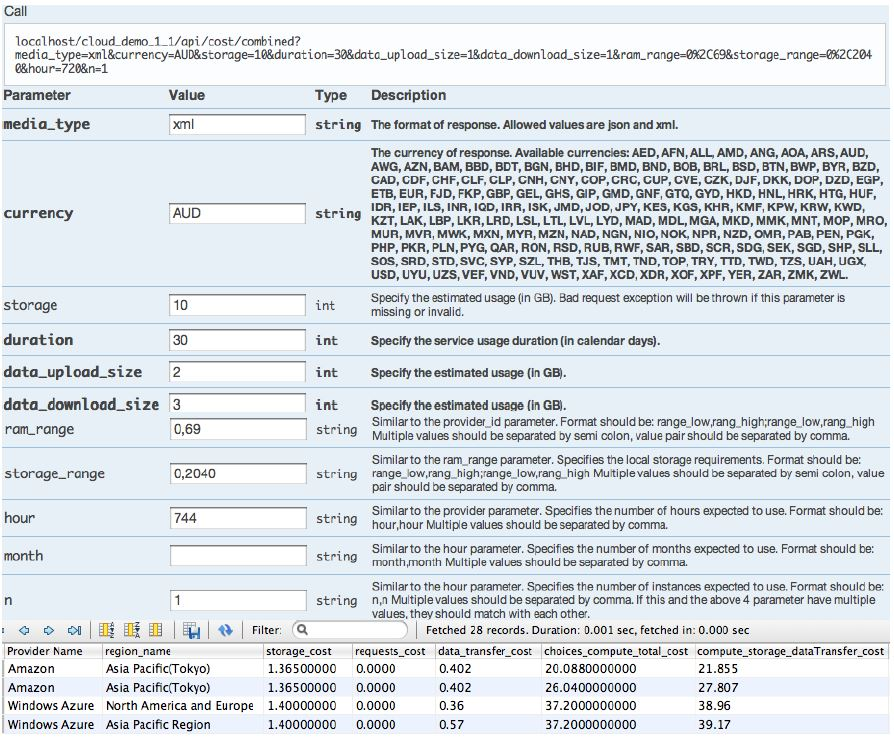
\includegraphics[width=\textwidth,keepaspectratio]{Figures/system/CloudRecommender/ResultOfSelectionForComputeStorageNetwork.jpg}
  \caption{Result of selection process for Compute, Storage and network services}
  \label{fig:ResultOfSelectionForComputeStorageNetwork}
\end{figure}

Fig. \ref{fig:ResultOfSelectionForComputeStorageNetwork} shows another
example which selects compute, storage, and network using the RESTful API. The
selection criteria include 1 compute service instance (shown as "n=1"):
0<Ram<=69, 0<=local storage<=2040, number of hours to be used per month 744.
The selection results are displayed at the end of the figure.

Due to high inter-cloud data transfer cost overhead and communication delay, our
recommender logic does not consider the combination of services from multiple
providers. For example, the CloudRecommender will not select and combine compute
service from Amazon with storage service from Azure. 
Similarly, some provider charge for data transfer across their
own services that are hosted at different regions. For example, data transferred
between Amazon services in different regions are charged as “Internet Data Transfer”
on both sides of the transfer. We currently choose to put all services in the same
region. In future we may extend our recommendation logic to allow users to choose
between different regions for each service type (if necessary). Additionally providers
often offer discounted price for higher usage, keeping all data together means higher
usage which can consume a cheaper price tier. Network services are always bundled
with either compute or storage service as it is impossible to consume other services
without incurring network costs.

\subsection{Case Studies}
\label{sec:case_studies}
Gaia is a global space astrometry mission with a goal of making the largest, most precise three-dimensional map of our Galaxy by surveying more than one billion starts. For the amount of images produced by the satellite (1 billion stars $\times$ 80 observations $\times$ 10 readouts), if it took one millisecond to process one image, it would take 30 years of data processing time on a single processor. Luckily the data does not need to be processed continuously, every 6 months they need to process all the observations in as short a time as possible (typically two weeks) \cite{GaiaCaseStudy}.
Hypothetically speaking say they choose to use 120 high CPU and memory VMs. The example search via CloudRecommender is shown in Fig. \ref{fig:GaiaCaseStudy}. With each VM running 12 threads, there were 1440 processes working in parallel. This will reduce the processing time to less than 200 hours (about a week).

\begin{figure}
  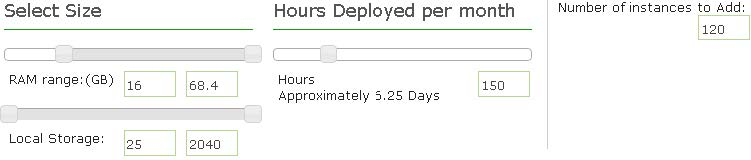
\includegraphics[width=\textwidth,keepaspectratio]{Figures/system/CloudRecommender/GaiaCaseStudy.jpg}
  \caption{Example input parameter values.}
  \label{fig:GaiaCaseStudy}
\end{figure}

In this case since data can be moved into/out of the cloud in bulk periodically, FedEx hard drive may be preferred over transferring data over the internet.

Promotional offers may not matter much in this case compare to the huge time and capital investment savings. But it makes a big difference for small business (or start ups) running a website.

Another example usage is sites with large continuous data input and processing need like Yelp. Everyday Yelp generates and stores around 100GB of logs and photos; runs approximately 200 MapReduce jobs and processing 3TB of data \cite{YelpCaseStudy}. Yelp.com has more than 71 million monthly unique visitors \cite{YelpFactsheet}. The average page size of a typical website is about 784 kB \cite{Pingdom}. So the estimated data download traffic is about 51TB per month if every unique user only views one page once a month. Fig. \ref{fig:YelpCaseStudy} shows a sample search for the above mentioned scenario.

\begin{figure}
  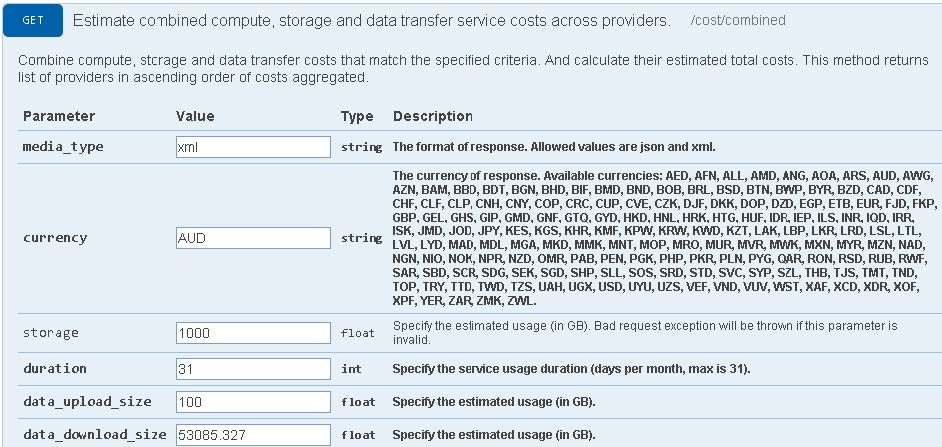
\includegraphics[width=\textwidth,keepaspectratio]{Figures/system/CloudRecommender/YelpCaseStudy.jpg}
  \caption{Example parameters for REST API.}
  \label{fig:YelpCaseStudy}
\end{figure}

% \includepdf[pages=2-,pagecommand={}]{papers/3.pdf}


%----------------------------------------------------------------------------------------
%	CONCLUSION
%----------------------------------------------------------------------------------------

\chapter{Conclusion}
\label{cha:conclusion}
We conclude our contributions and point out future directions in this area.

\section{Impact}
This thesis mainly considers the problem of automatic Cloud IaaS service discovery and comparison.
It also explored ways to forecast cloud usage in order to estimate cost, thus providing optimal Cloud deployment options (i.e. which provider, total cost, what kind of servers, how many of them, the expected average network performance e.t.c).  

Although elasticity, cost benefits and abundance of resources motivate many organizations to migrate their enterprise applications to the Cloud, end-users (e.g., CIOs, scientists, developers, engineers, etc.) are faced with the complexity of choosing the right set of Cloud services for deploying their applications. Manually reading Cloud providers’ documentation to find out which services are suitable for building their Cloud-based application is a cumbersome task for decision makers. The multi-layered organization (e.g., SaaS, PaaS, and IaaS) of Cloud Services, along with their heterogeneous types and features makes the task of service identification a hard problem. For example, EC2 instances, virtual/compute/cloud servers are all the same thing; S3, Cloud files, object store all refers to storage. In addition to the actual price difference for similar service among various providers, a range of pricing models for how services are charged are also making it more complicated, like Pay as you go, Spot Instance or bidding, two part tariff, block-declining, free for a period or discounted with bulk buy.Hence for dealing with the complexity of choosing from large number of heterogeneous cloud services from diverse providers, end-users need access to specialized intermediaries which can act as a “one-stop-shop” for procuring and comparing Cloud services. 

We addressed the aforementioned problems by introducing a number of techniques with their implementation to form a Cloud recommendation tool-set which enables simplified and intuitive cloud service selection. It allows multi-criteria search on infrastructure cloud offers across different cloud providers.It is a semi-automated approach aids in the network-QoS-aware 
selection of cloud services, along with a unified domain model that
is capable of fully describing infrastructure services in cloud
computing. This approach takes into account of real-time and variable network QoS constraints,
and applies a utility function that combines multiple selection criteria
(e.g., the total cost, the maximum size limit for
storage, and the memory size for compute instance)
pertaining to storage, compute, and network services.

The Cloud recommendation tool-set is expected to be of significant value to end-users, who are presently:
\begin{enumerate}
\item considering migrating their applications to Cloud services for cost savings.
\item hard-pressed to understand the cost and benefits of moving to Cloud, especially when the market evolves so rapidly.
\end{enumerate}

\section{Contributions}
The cloud has great potential for a large variety of users with diverse needs, but the selection of a the right provider is crucial to this end. Aiming to eliminate potential bottlenecks that limit the ability of general users to take advantage of cloud computing, we present a comprehensive solution set, which allows user to make multi-criteria selection and comparison on IaaS offers considering QoS. We hope our research will drive even greater adoption of the cloud and boost the expansion of the cloud hosted applications. 

\subsection{Standardization of Terminologies Concepts and Processe in Cloud}
We have proposed ontology for classifying and representing the configuration information related to Cloud-based IaaS services including compute, storage, and network. The proposed ontology is comprehensive as it captures both static confiugrations and dynamic QoS configurations on the IaaS layer.

By proposing the CoCoOn Ontology, and implementing relevant tool,
empowering automatic cross linking data from different providers as well as external domains,
i.e. Geo Locations, Units, Business Service (GoodRelations).
Thus, unify the process of selection and comparison Cloud IaaS Services.

This work will also help readers in clearly understanding the core IaaS-level Cloud computing concepts and inter-relationship between different service types. This in turn may lead to a harmonization of research efforts and more inter-operable Cloud technologies and services at the IaaS layer.

\subsection{Network-Aware QoS Computation}
A generic service that helps in collecting network QoS values
from different points on the Internet (modeling a big data source
location) to the cloud data centers.

\subsection{Problem Formulation}
A clear formulation of the research problem by identifying the most important
cloud service selection criteria relevant to specific real-time
QoS-driven applications, selection objectives, and cloud service
alternatives.

\subsection{Multicriteria Optimization}
An analytic hierarchy process (AHP)-based decision making 
(service selection) technique that handles multiple
quantitative (i.e., numeric) and qualitative (a descriptive and
nonnumeric, such as location, CPU architecture, i.e., a 32- or
64-bit operating system) QoS criteria. The AHP determines
the relative importance of criteria to each user by conducting
pairwise comparisons.

\subsection{Resource Usage Estimation based on Benchmarking and Performance Modelling}

\subsection{Cloud Recommendation Toolset}
We proposed a declarative system (CloudRecommender) that transforms
the cloud service configuration selection from an ad-hoc process that involves
manually reading the provider documentations to a process that is structured, and to a
large extend automated. Although we believe that CloudRecommender leaves scope
for a range of enhancements, yet provides a practical approach. We have implemented
a prototype of CloudRecommender and evaluated it using an example selection
scenario. The prototype demonstrates the feasibility of the CloudRecommender
design and its practical aspects.

\section{Reflection and Future Work}
There are a number of possible extensions that can be made to CoCoOn:
\begin{enumerate}
    \item More providers should be included.
    \item Using Custom Datatypes \texttt{cdt:ucum} \cite{lefrancois_eswc_2018} to define custom units in CoCoOn, and so it can be implemented to handle conversions properly.
    \item Improve \href{https://github.com/miranda-zhang/cloud-computing-schema/tree/master/example/geonames_rdf/azure}{mapping regions to Geoname dataset}.
    \item Model various discounts.
\end{enumerate}

For the current implementation of the
CloudRecommender system, we have defined the Cloud
infrastructure layer (IaaS), providing concepts and relations
that are fundamental to the other higher-level layers.
For future work, to cover both PaaS
and SaaS layers would be a nice inclusion.
In terms of system implementation, we could migrate the infrastructure services definitions to a RDF database and use, for example, SPIN templates \cite{SPIN} to encode our procedures in SPARQL \cite{SPARQL}.
Moreover, it would also be nice to capture the dependency of services across the layers. For example, investigating concepts and relationships for identifying the dependencies between compute service (IaaS) configurations and the type of appliances (PaaS) that can be deployed over it. For example, before mapping a MySQL database appliance (PaaS) to a Amazon EC2 compute service (IaaS), one needs to consider whether they are compatible in terms of virtualization format. 
Other parameters worth including into the decision making process are SLA and legal compliance \cite{mouratidis2013framework} information.

Another avenue that we would like to explore is spot instance bidding/auction market. There are a number of
research focus on service brokerage that can be of good synergy to our work.
 
 
%----------------------------------------------------------------------------------------
%	APPENDICES
%----------------------------------------------------------------------------------------

\appendix % Cue to tell LaTeX that the following "chapters" are Appendices

% Include the appendices of the thesis as separate files from the Appendices folder
% Uncomment the lines as you write the Appendices

%\chapter{Publications Recap}
Revisions on old works.

\section{Investigating decision support techniques for automating Cloud service selection}
\label{paper:proposal}
This paper briefly introduces features of Cloud Infrastructure as a Service, then gives an overview on the generally faced challenges by Cloud users in the first step of picking from various options. Problems depicted are grouped under the following areas:

\begin{enumerate}
	
  % 1
  \item \label{itm:service_identification_representation}
  Automatic service identification and representation.   
  
  \begin{enumerate}[label*=\arabic*.]
  
  	% 1.1
    \item \label{itm:service_discovery} 
    How to automatically fetch service description published by Cloud providers and present them to decision makers in a human readable way?
    % 1.2
    \item \label{itm:ontology}
    Can we develop an unified and generic Cloud ontology to describe the services of any Cloud provider which exists now or may become available in the future?
  \end{enumerate}
  
  % 2
  \item \label{itm:selection_comparison}
  Optimized Cloud Service Selection and Comparison.
  
  \begin{enumerate}[label*=\arabic*.]
  	% 2.1
    \item \label{itm:comparison}
    How well does a service of a Cloud provider perform compared to the other providers? 
    % 2.2
    \item \label{itm:compatibility}
    Which Cloud services are compatible to be combined or bundled together?
    % 2.3
    \item \label{composition}
    How to optimize the process of composite Cloud service selection and bundling?
  \end{enumerate}  
  
  % 3
  \item \label{itm:interface}
  Simplified interfaces for Cloud Service Selection.
  
  \begin{enumerate}[label*=\arabic*.]
    \item How to develop interfaces that can transform low, system-level programming to easy-to-use drag and drop operations? 
    \item Will such interfaces improve and simplify the process of Cloud Service Selection and Comparison? 
  \end{enumerate} 
  
\end{enumerate}

The research required to address question \ref{itm:service_discovery} is discussed in paper \ref{paper:ontology} . One option to address the knowledge discovery problem is everyone follows a unified standard, then information can be automatically fetched, but this requires considerable efforts for Cloud providers. Otherwise, a software for harvesting information needs constant human update to accommodate every single change in Cloud providers’ websites. 

A few sub questions are identified under each area, but there is not enough time to address all of them during the course of this research. Under question \ref{itm:selection_comparison}, my research is primarily focused on solving \ref{itm:comparison}. Service composition related questions may be  investigated in future work.

\subsection{Remark}
Some  of the works reviewed in this paper are outdated, for example, Yuruware revised it's scope to focus on cloud disaster recovery now, which is quite different from our research. Similarly, some of the early days Cloud Providers no longer provide public IaaS services. For example, GoGrid was included in our initial study, but they have shifted its focus to provide consultation, despite the fact that they still claims to have data center around the globe, their business now days are mostly helping businesses to architect, deploy and manage multi platform hybrid IT solutions (i.e. in public, private and hybrid clouds). However, the non-standardized terminology problem still largely remains with other cloud providers.
Although Cloud have been around a while now, the market environment of IaaS is still changing rapidly, with new vendors (e.g. DataCentred, atlantic.net)and services (e.g. Mobile and Internet of Things related services) introduced, the corresponding concepts also evolves as a result. However, Amazon Web Service has the trend to become the de Facto Standard, at the same time, big name competitors (i.e. Hewlett-Packard, IBM) would very much like to knock Amazon o its perch. Therefor, there is still a lot of discussion around building the actual de jure Standard.

Although we didn't conduct surveys, We analyzed a lot of case studies published by the providers. It is more time efficient and easier compare to surveys, with no need to obtaining ethics approval. Those case studies are based on real life businesses scenarios, from a broad range of disciplines.

Genetic Algorithm(GA) was initially proposed because it shows some promising results for a problem another student of my supervisor is working on \cite{CloudGenius}. But after some experimentation, we realized that Genetic Algorithm(GA) is not appropriate for our problem. GA does not always find the global optima, it's
relatively time-consuming and does not scale well with complexity (i.e. search space grow
exponentially for large number of Cloud service options) \cite{GA_wiki}. But our current approach will find the global optima and is more efficient.

Deploy application in Cloud involves a lot of complex low level programming, thus making
it a time consuming and challenge task even with one Cloud platform, let along manage a
hybrid Cloud environment. Among the various attempts targeting this Cloud orchestration
problem, Cloudify \cite{Cloudify} seems to be a promising solution. Since Cloud orchestration is not the
main focus of my research, my work would concentrate only on providing related interface
for comparing Cloud Services. At the time of writing this paper, we considered integrating
the proposed Cloud Recommender with a Cloud orchestration tool as possible future
work.
 
There are some research works using AHP to solve cloud related decision problem. One
paper combined AHP with benefit-cost-opportunity-risk (BCOR) analysis to select the best
cloud computing deployment model \cite{AHP_BCOR}, but it did not consider the complexity of dealing with hundred thousands of public cloud options, it only provides a high level methodology, specifically to decide whether to choose public, private, or hybrid cloud deployment.  
Another paper \cite{CloudGenius} combined AHP and GA to automate the migration of web application clusters to public clouds. But it is looking at VM image bundles, in comparison,
CloudRecomender is comparing IaaS offers.

In Chapter \ref{cha:selection}
we employed AHP to find th optimal result considering
multiple conflicting criteria. We did not try the simple additive weighting approach,
because despite the "simple" in its name, computational wise it is not much a simpler than
AHP. Space pruning is not implemented since we decide to follow the declarative programming
paradigm, which allows us to taking advantage of the optimized query operations in SQL
(e.g. select and join). Knowing that modern databases often implement those operation
very efficiently, it is not within our scope to improve it further, instead we tried cache
query results for repeated query and pre-compute some values to reduce computation time.

Although there is not a full satisfaction study, we made numerous attempts to 
get evaluations from research community and industry. We have presented our system 
at various conferences (CloudCom, GECON), competitions
(make into the finalist of NASSCOM Inovation Student Awards) and to our research
partners (Institute of Remote Sensing and Digital Earth, Chinese Academy of Sciences add
Myriads research team, INRIA). We have modified our system according to their
feedbacks. 

\subsection{Attribution statement}
The candidate undertook the research and analysis, and wrote the chapter. 
Dr Ranjan provided valuable guidance. Dr Haller provided insights on semantic modeling. 
Dr Georgakopoulos inputs ideas on experimental result validation. 
Dr Strazdins provided reflections and comments through out the writing of this paper.

\section{An Ontology based System for Cloud Infrastructure Services Discovery}
\label{paper:ontology}
This paper explores ontology based methods to address the research question identified 
in section \ref{subsec:service_discovery}. 

An ontology was developed using semantic Web languages like the Resource Description Framework (RDF) and the Web Ontology Language (OWL), thus answered question \ref{itm:ontology}.
The semantic web initiative is proposed to simplify the information discovery process on the web, to take advantage of existing effort, an OWL-based ontology model have been developed as an attempt to address the previously mentioned knowledge discovery and data standardization problem. In particular, the Cloud Computing Ontology (CoCoOn) defines functional and non-functional concepts, attributes and relations of infrastructure services. This ontology facilitates the description of Cloud infrastructure services; and through mappings from provider descriptions, facilitates the discovery of infrastructure services based on their functionality.
By modeling of service descriptions published by Cloud providers according to the developed ontology, this paper validates the expressiveness of ontology against the most commonly available infrastructure services including Amazon, Microsoft Azure etc.

\subsection{Attribution statement}
The candidate undertook most of the conception design and analysis. 
Dr Ranjan provided valuable guidance. 
Dr Haller added expertise in Web Ontology Language, and led the implementation of CoCoOn.
Dr GeorgakopoulosI and Dr Nepal provided reflections and comments through out the writing of this paper.
Dr Menzel provided useful suggestions by sharing experience on design of decision support system for web server cloud migration.
  
\section{Discovery-Driven Service Oriented IoT Architecture}
\label{paper:soa_iot}

This paper discusses the problem of service and data discovery in the context of Internet of Things. This resembles the service discovery problem discussed in section \ref{subsec:service_discovery}.

Cloud computing has proved to be the de facto standard for delivering internet-based application services in particular supporting IoT applications and services. Such applications will require dynamic mash-ups of things and services to be created across the IoT layers. This leads to the most important and demanding challenge i.e. how to interoperate and integrate data to suit the application needs autonomously? Just like how the human brain can perceive and integrate things seamlessly to infer contextual insights, the question that will govern the IoT ecosystem is, what and how will IoT deliver to me?

This paper presents a vision of a future IoT system architecture that is driven by service discovery across every layer of the IoT system. This paper identified the  gap in current IoT architectures, that is disconnected efforts focusing on specific layers of the IoT stack, but missing the integrate service oriented concepts across the layers allowing autonomous composition of IoT applications. The work presented in this paper addresses these problem by proposing a blue print architecture for a discovery driven service oriented IoT architecture.
This paper also presents the challenges in discovery, description and representation of service and integration. The proposed blueprint architecture aims to address these challenges by embedding of discovery and integration of services at each of the devices, data and applications layers of the abstract IoT model. 
Finally, this paper provided discussions into how the proposed model can be realized by taking into consideration of some previous work in the areas of device discovery in OpenIoT and cloud discovery in Cloud Recommender.

\subsection{Attribution statement}
This is a joint paper that the candidate was involved, but the work primarily was conducted by the leading authors.

\section{City Data Fusion: Sensor Data Fusion in the Internet of Things}
\label{paper:ct_data_fusion}
This paper addresses major open research issues related to sensor data fusion, likewise to paper paper \ref{paper:soa_iot}, some of the problems touched by this paper are related to research question in section \ref{subsec:service_discovery}.  

This paper highlights the importance of sensor data fusion in IoT application such as smart
cities applications. Mainly, data fusion operations can be applied at two levels: cloud level and within the network level. Cloud level devices have access to unlimited resources and hence has the capability to apply complex data mining algorithms over the data generated by large number of lower level sensors. After understanding the environment, the cloud can generate actions that need to be taken appropriately. In-network sensor data fusion is important to reduce the data transmission cost. However, low-level nodes may not have the full view of the environment. In such situation, a middle-ware such as CloudRecommender would be needed to enable complex cooperative operations.

\subsection{Attribution statement}
This is a joint paper that the candidate was involved, but the work primarily was conducted by the leading authors.

\subsection{A Declarative Recommender System for Cloud Infrastructure Services Selection}
\label{paper:single_criteria}

This paper addresses question \ref{itm:service_identification_representation} and \ref{itm:interface}. It explains the implementation of CloudRecommender, a decision support system based on our ontological model for the selection of infrastructure Cloud service configurations. The benefits to users of CloudRecommender include, for example, the ability to estimate costs, compute cost savings across multiple providers with possible trade offs.

Though branded calculators are available from individual cloud providers, such as Amazon, Azure and GoGrid, for calculating service leasing cost, it is not easy for users to generalize their requirements to fit different service offers (with various quota and limitations) let alone computing and comparing costs, thus our system is needed.

The ontology CoCoOn proposed in paper \ref{paper:ontology} was implemented as a relational model. It is then populated with data collected from various Cloud providers' websites. We also profiled the corresponding QoS statistics of those services. By extending CoCoOn into a decision support system, with reasonable interface, we partially addressed question \ref{itm:selection_comparison} and \ref{itm:interface} .

CloudRecommender formally captures the domain knowledge of services using a declarative logic-based language, so procedures in CloudRecommender are transactional and well defined in SQL semantics. The CloudRecommender system also leverages the Web-based widget programming technique that transforms drag and drop operations to low-level SQL transactions. It provides an user-friendly service interface that maps user requirements to available infrastructure services.

\subsection{Remark}
This initial prototype did not apply optimization techniques, single objective search was implemented.

\subsection{Attribution statement}
The candidate undertook the majority of the research work, from design, implementation, data collection to analysis and wrote the chapter. 
Dr Ranjan provided valuable guidance. 
Dr Nepal and Dr Menzel provided advice on all sections.
Dr Haller added insights on how to implement OWL-ontology as relational model.

\section{Investigating Techniques for Automating the Selection of Cloud Infrastructure Services}

Similar to paper \ref{paper:single_criteria}, the work of this paper primarily addresses research problem \ref{itm:service_identification_representation} and \ref{itm:interface}, it further illustrates the detailed design of CloudRecommender after the latest improvements.

This paper gives an overview of previous work, which will help readers in clearly understanding the core IaaS-level Cloud computing concepts and inter-relationship between different service types.

This paper also revised the proposed ontology for classifying and representing the configuration information related to Cloud-based IaaS services. The corresponding  implementation is updated, it further expose a RESTful (REpresentational State Transfer) APIs (application programming interface) that help external applications to programmatically compose infrastructure cloud services based on the CloudRecommender selection process.

\subsection{Attribution statement}
This paper is an extended journal version of a previous conference paper.
The candidate undertook the work for extending the original system 
(including both model design and implementation) and wrote about the new work.
Dr Ranjan provided valuable guidance.
The other co-authors assisted in writing.

\section{An Infrastructure Service Recommendation System for Cloud Applications with Real-time QoS Requirement Constraints}
This paper addresses research problem \ref{subsec:service_comparison} . 

In order to select the best mix of service offering from an abundance of possibilities, application owners must simultaneously consider and optimize complex dependencies and heterogeneous sets of criteria (price, features, location, etc.). 
For instance, it's not enough to just select optimal cloud storage service, corresponding computing capabilities (at where data is located, so no additional data transfer is needed) are essential to guarantee that one is able to process the data as fast as possible while minimizing the cost. 
Matching results to decision makers’ requirements may also involves bundling of multiple related Cloud services, computing combined cost (under different billing models and discount offers), considering all possible (or only valuable) alternatives and multiple selection criteria.

To this end, we present multi-criteria decision making technique that builds over well known AHP method. AHP handles multiple quantitative (i.e. numeric) as well as qualitative (descriptive, non numeric, like location, CPU architecture: 32 or 64 bit, operating system) criteria. It determines the relative importance of criteria to each user by conducting pair-wise comparisons. The proposed technique is applicable to selecting Infrastructure as a Service (IaaS) cloud offers, and it allows users to define multiple design-time constraints. These requirements are then matched against our knowledge base to compute possible best fit combinations of cloud services at IaaS layer. 

A number of research and commercial projects provide simple cost calculation or benchmarking and status monitoring, but none is capable to consolidate all aspects and provide a comprehensive ranking of infrastructure services. For instance, CloudHarmony \cite{cloudharmony_speedtest} provides benchmark results without considering cost, Cloudorado \cite{Cloudorado} calculates the price of IaaS-level CPU services based on static features (e.g., processor type, processor speed, I/O capacity, etc.) while ignoring dynamic QoS features (e.g. latency, throughput etc.). Another project is the Swinburne University's Smart Cloud Broker Service \cite{SwinburneCloudBroker}. From the screen cast they released we can tell that their benchmarking is done in real-time, which means users have to wait for the results to come back. We have considered this kind of situations, but decided to collect the benchmarking result beforehand. Because this way no matter how many cloud providers users want to compare against, they can still get the result with minimum (or no) waiting time. Another reason we choose to do it this way is because, at any particular point in time, the network benchmark result is not conclusive as performance fluctuates during time, so we use aggregated average which is a more reliable overall indication.

There are two distinctive features the proposed solution provide during ranking and comparing various vendor services: 
\begin{enumerate}
	\item
	Allow users to choose to include the QoS requirements during comparison.
	\item
    When users want to take into account mixed qualitative (e.g. hosting region, operating system type) and quantitative criteria, we apply the Analytic Hierarchy Process (AHP) to aggregate numerical measurements and non numerical evaluation. Results are personalized according to each user's preferences, because AHP takes users' perceived relative importance of criteria (pair-wise comparisons) as inputs.
\end{enumerate}

\subsection{Attribution statement}
The candidate led the research work, undertook most of the problem formulation, data analysis, implementation, experimentation and writing.
Dr Ranjan provided valuable guidance on all aspects. 
Dr Menzel added expertise in AHP, and helped with the implementation.
Dr Nepal and Dr Strazdins provided advice on conception design and architecture.
Dr Jie and Dr Wang assisted with formulation.

\section{Early Observations on Performance of Google Compute Engine for Scientific Computing}

This paper’s evaluation work on Google Compute Engine (GCE) is relevant to research problem \ref{subsec:service_comparison}.

In 2013, public Cloud services was still new for most, and it was regarded as a potential and encouraging paradigm for scientific computing. Back then, Google Compute Engine (GCE) was just available, and claimed to support high-performance and computationally intensive tasks, while little evaluation studies can be found to reveal GCE’s scientific capabilities. Considering that fundamental performance benchmarking is the strategy of early-stage evaluation of new Cloud services, we followed the Cloud Evaluation Experiment Methodology (CEEM) to benchmark GCE and also compare it with Amazon EC2, to help understand the elementary capability of GCE for dealing with scientific problems. 

The experimental results and analyses show both potential advantages of, and possible threats to applying GCE to scientific computing. Following the same evaluation methodology, different evaluators can replicate and/or supplement this fundamental evaluation of GCE. Based on the fundamental evaluation results, suitable GCE environments can be further established for case studies of solving real science problems.

The potential advantages of using GCE: Relatively high memory data throughput. Different GCE types seem to have consistent type of virtual memory. Relatively fast storage transaction speed.
Relatively fast computation transaction speed with single process. Relatively computationally economic, given generally high computation performance/price ratio.

The possible threats to using GCE: Relatively low communication data throughput between
US and European data centers. Distributed computing crossing both data centers may need to be well balanced. Considerable variability of storage performance. GCE seems to have a lack of dedicated storage cache. Considerable variability of computation transaction
speed on high memory VM type. Relatively poor (original) scalability when switching
process numbers on individual VMs. GCE’s hyperthread-based virtual core seems not a suitable mechanism for parallel computing.

\subsection{Attribution statement}
The candidate helped with the experiments, including setting up the environment on both AWS and GCE, data collection of repeated tests.

\section{An Overview of Cloud Based Content Delivery Networks: Research Dimensions and State-of-the-Art}

This paper written in 2015, presents a state-of-the-art survey on current commercial and research/academic Cloud-based Content distribution networks (CCDNs). Some of the existing challenge provides motivation for Cloud recommendation service.

Cloud CDN providers are mostly based on one cloud platform and lacks support for the emerging form of content distribution namely dynamic user-generated content. Since, the solutions are based on a single cloud providers, the services lack consideration for cost models when taking advantage of cloud content storage spanning multiple cloud providers. Further, most solutions lack support for penalization at user level. 

The future CCDN should be based around the need to support user created content and demonstrates ability to support hybrid cloud platforms and addressing the challenges such as QoS, SLA, costing introduced by hybrid clouds.

\subsection{Attribution statement}

\section{Service recommendation based on Benchmarking and Analytical Performance Model}
\subsection{Attribution statement}
%----------------------------------------------------------------------------------------
%	BIBLIOGRAPHY
%----------------------------------------------------------------------------------------

\printbibliography[heading=bibintoc]

%----------------------------------------------------------------------------------------

\end{document}  
